\documentclass[12pt]{report}

% Paquetes LaTeX y estilos globales
\usepackage[utf8]{inputenc}
\usepackage{multicol}
\usepackage{xcolor}
\usepackage{subfigure}
\usepackage[spanish,es-tabla]{babel}
\usepackage[utf8]{inputenc}
\usepackage{graphicx}
\usepackage{titlesec}
\usepackage[bookmarks,breaklinks,colorlinks=true,allcolors=blue]{hyperref}
\newcommand{\issue}[1]{\textbf{\href{https://github.com/frangago71/quizzie-TFG/issues/#1}{\##1}}}
\usepackage{listings}
\usepackage{inconsolata}
\usepackage{float}
\usepackage{mathpazo} % Fuente Palatino
\usepackage[labelfont=bf]{caption}

\usepackage[square,numbers]{natbib}
\usepackage[nottoc,notlof,notlot]{tocbibind}  % Mete la bibliografía como capítulo en la TOC, los parámetros excluyen los otros índices de aparecer también
\usepackage{geometry}
\usepackage{amsmath}
\usepackage{parskip}
\usepackage[official]{eurosym}
\usepackage{todonotes}
\usepackage{csquotes}
\usepackage{tocbasic}  % Estilos de la TOC
\usepackage{tabularx}  % Tablas con ancho total ajustable
\usepackage{booktabs} 
\usepackage{amssymb}

\usepackage{tikz}
\usetikzlibrary{trees}
\usepackage{longtable}
\usetikzlibrary{positioning, trees}
\usepackage{pgfgantt}
\usepackage{pgfplots}
\pgfplotsset{compat=1.18}
\pgfdeclarelayer{behind}
\pgfsetlayers{background,behind,main}

\usepackage{rotating} 
\usepackage{array}

\usepackage{dirtree}

\usepackage[title]{appendix} 

\usepackage{pdfpages}

\usepackage{newfloat}

\usepackage{makecell}

\usepackage{pifont}
% Formato del título de capítulos y secciones
\titleformat{\chapter}[block]{\normalfont\huge\bfseries}{\thechapter.}{.5em}{\Huge}[\vspace{2pt}{\titlerule[2pt]}]

\titlespacing*{\chapter}{0pt}{-19pt}{25pt}

\titleformat{\section}[block]{\normalfont\Large\bfseries}{\thesection.}{.5em}{\Large}

\titleformat{\part}[block]{\titlerule[2pt]\normalfont\Huge\bfseries\centering}{Parte \Roman{part}\\\vspace{15pt}}{0pt}{\Huge}[\vspace{2pt}{\titlerule[2pt]}]

% Tamaños y estilos de elementos en la TOC
\DeclareTOCStyleEntry[
    linefill=\bfseries\TOCLineLeaderFill,
    beforeskip=12pt,
    entrynumberformat=\chapterprefixintoc,
    entryformat=\chaptertocformat,
    pagenumberformat=\chaptertocformat,
    dynnumwidth
]{tocline}{chapter}

\DeclareTOCStyleEntry[
    % linefill=\bfseries\TOCLineLeaderFill,
    beforeskip=30pt,
    entrynumberformat=\chapterprefixintoc,
    entryformat=\parttocformat,
    pagenumberformat=\partpagetocformat,
    numwidth=0pt
]{tocline}{part}

\newcommand\chaptertocformat[1]{\large{\textbf{#1}}}%
\newcommand\chapterprefixintoc[1]{#1}%
\newcommand\parttocformat[1]{\Large{\textbf{#1}}}%
\newcommand\partpagetocformat[1]{} % Don't print the page number for parts

% Alias para estilos de texto comunes
\newcommand{\negritas}[1]{\textbf{#1}}
\newcommand{\cursiva}[1]{\textit{#1}}
\newcommand{\codigo}[1]{\texttt{#1}}

% Formato del código fuente con lstlisting
\lstset{
  basicstyle=\ttfamily,
  breaklines=true,
}

% Márgenes
\geometry{
    a4paper,
    margin=2.75cm
}
\setlength{\marginparwidth}{2cm}

% Limite de profundidad del índice
\setcounter{tocdepth}{2}

% Eliminar el guionado
\tolerance=1
\emergencystretch=\maxdimen
\hyphenpenalty=10000
\hbadness=10000

% Indentación de párrafos
\setlength{\parindent}{.75cm}

\renewcommand{\lstlistingname}{Extracto de código}
\renewcommand*{\lstlistlistingname}{Índice de extractos de código}

\usepackage{newfloat}
\usepackage{caption}

\DeclareFloatingEnvironment[
    fileext=loe,
    listname={Índice de evidencias},
    name=Evidencia,
    placement=H,
    within=chapter
]{evidence}

% Definición de colores personalizados para los enlaces
\definecolor{primaryCyan}{RGB}{85, 204, 170}
\definecolor{primaryMagenta}{RGB}{169, 70, 171}
\definecolor{secondaryCyan}{RGB}{0, 121, 118}
\definecolor{secondaryMagenta}{RGB}{102, 20, 101}

\hypersetup{
    colorlinks=true,       
    linkcolor=primaryMagenta,   % Color para referencias internas 
    citecolor=secondaryCyan,   % Color para citas bibliográficas 
    urlcolor=primaryCyan      % Color para direcciones web 
}

% Comandos para establecer variables
\newcommand{\setTitle}[1]{\def\tfgTitle {#1}}
\newcommand{\setAuthor}[1]{\def\tfgAuthors {#1}}
\newcommand{\setDegree}[1]{\def\tfgDegree {#1}}
\newcommand{\setSupervisor}[1]{\def\tfgSupervisor {#1}}
\newcommand{\setDepartment}[1]{\def\tfgDepartment {#1}}
\newcommand{\setMonth}[1]{\def\tfgMonth {#1}}
\newcommand{\setYear}[1]{\def\tfgYear {#1}}
\newcommand{\setDedication}[1]{\def\tfgDedication {#1}}

\newcommand{\covRed}[1]{\textcolor{red!80!black}{\textbf{#1}}}
\newcommand{\covCross}{\textcolor{red!80!black}{\scalebox{1.4}{\textbf{\texttimes}}}}
\definecolor{covYellow}{RGB}{218,165,32}
\newcommand{\covYellow}[1]{\textcolor{covYellow}{\textbf{#1}}} 
\newcommand{\covPartial}{\textcolor{covYellow}{\raisebox{0.25ex}{\scalebox{1.8}{\textbf{\texttildelow}}}}}
\newcommand{\covGreen}[1]{\textcolor{green!60!black}{\textbf{#1}}}
% \newcommand{\covCheck}{\textcolor{green!60!black}{\textbf{\checkmark}}}
\newcommand{\covCheck}{\textcolor{green!60!black}{\ding{51}}}       
\definecolor{bashYellow}{RGB}{204, 204, 0} 
\newcommand{\bashYellow}[1]{\textcolor{bashYellow}{\textbf{#1}}}
\definecolor{bashGrey}{RGB}{140, 140, 140}
\newcommand{\bashGrey}[1]{\textcolor{bashGrey}{\textbf{#1}}}
\newcommand{\cliPrompt}{\textcolor{bashGrey}{\textbf{>}}}


\lstdefinestyle{terminal}{
    language={},
    basicstyle=\fontsize{12pt}{13.8pt}\ttfamily\color{black},
    keywordstyle=\color{black},
    commentstyle=\color{black},
    stringstyle=\color{black},
    identifierstyle=\color{black},
    numbers=none,
    frame=none,
    columns=fullflexible,
    keepspaces=true,
    showstringspaces=false,
    escapeinside={(*@}{@*)}
}
\lstset{style=terminal}

\makeatletter
\renewcommand{\@pnumwidth}{2.2em}
\renewcommand{\@tocrmarg}{2.5em}
\makeatother


\setTitle{Quizzie - Plataforma multidispositivo para la realización y gestión dinámica de tests educativos}
\setAuthor{Francisco Gago Vázquez}
\setDegree{Grado en Ingeniería Informática - Ingeniería del Software} 
\setSupervisor{Jesús Moreno León} 
\setDepartment{Lenguajes y Sistemas Informáticos}
\setMonth{octubre} 
\setYear{2025/26} 

\setDedication{A mis padres y a mi hermana, por estar siempre ahí. Gracias por cuidarme todos estos años, por vuestra paciencia infinita en las épocas más difíciles y por ser mi apoyo constante en cada paso del camino. Este trabajo también es vuestro.}

\begin{document}

    % Portada y secciones no numeradas
    \input{sections/00_portada}
    \chapter*{Agradecimientos}

En primer lugar, quiero expresar mi más sincero agradecimiento a mi tutor, Jesús Moreno, por su constante guía, cercanía y disponibilidad a lo largo de este proyecto. Sus consejos, revisiones y criterio técnico han sido fundamentales para orientar el trabajo y llevar \textit{Quizzie} a buen puerto.

A todas las amistades y compañeros que me llevo de estos años de carrera. Superar cada curso, las entregas conjuntas y las semanas de exámenes ha sido infinitamente más fácil y enriquecedor gracias a vosotros, por tantas horas compartidas en las aulas y por los buenos momentos fuera de ellas.

Un agradecimiento muy especial para Marta y Paco. Gracias por estar siempre ahí durante los meses de desarrollo de este trabajo, por compartir tantos días en la biblioteca y, sobre todo, por aguantarme, escucharme y apoyarme cuando tocaba desconectar fuera de ella. Teneros cerca ha marcado la diferencia en este proceso.

Por último, a mis padres y a mi hermana. Aunque ya les dedico estas páginas, no puedo cerrar este proyecto sin agradecerles su apoyo incondicional, su paciencia y su confianza.
    \chapter*{Resumen}

La gamificación en el ámbito educativo se ha consolidado como un enfoque eficaz para fomentar el aprendizaje dinámico y agilizar las sesiones lectivas. No obstante, el análisis del mercado revela una brecha notable: las soluciones comerciales priorizan el entretenimiento a costa del rigor académico, limitan las analíticas exportables y propician el fraude por suplantación digital al permitir que estudiantes ausentes participen de forma remota compartiendo el código PIN de acceso. Por su parte, los cuestionarios de plataformas institucionales garantizan la formalidad evaluativa, pero sacrifican la inmediatez y la fluidez interactiva en el aula.

En este Trabajo de Fin de Grado se presenta \textit{Quizzie}, una plataforma multidispositivo concebida para la creación, realización y gestión dinámica de cuestionarios educativos en tiempo real. La arquitectura adopta un modelo cliente-servidor desacoplado, implementando una interfaz reactiva en React sobre Vite con TypeScript, desplegada en Vercel. El \textit{backend}, alojado en Render, se sustenta sobre un servidor asíncrono desarrollado en Python con FastAPI y gestionado mediante uv, apoyándose en una persistencia relacional ligera con SQLModel y SQLite. La comunicación bidireccional y síncrona de las salas se articula a través del protocolo \textit{WebSocket}. Como elemento innovador y factor diferencial, la plataforma incorpora un mecanismo de verificación de asistencia física basado en la generación de un código QR unívoco en el dispositivo del estudiante al concluir el test, el cual es escaneado por el docente para confirmar de manera inequívoca la presencialidad y registrar la calificación de forma instantánea. Asimismo, el diseño respeta el principio de minimización de datos del RGPD, permitiendo el acceso del alumnado sin registros tradicionales mediante el identificador institucional de la Universidad de Sevilla (\textit{uvus}).

El proyecto se ha abordado siguiendo un ciclo de vida completo de ingeniería del \textit{software}, estructurado mediante metodologías ágiles desde el análisis de requisitos y el modelado arquitectónico hasta la verificación exhaustiva de la solución. El resultado es un producto funcional, robusto y seguro, distribuido bajo licencia de código abierto MIT y concebido como una herramienta viable para su adopción en una amplia variedad de contextos formativos y docentes.

\vspace{0.5cm}

\textbf{Palabras clave:} Gamificación educativa, Tecnología educativa, Evaluación interactiva, Verificación presencial, Prevención de fraude digital, Control de acceso basado en roles (RBAC), Minimización de datos, Arquitectura cliente-servidor desacoplada, Comunicación bidireccional síncrona.
    \chapter*{Abstract}

Gamification in education has established itself as an effective approach to foster dynamic learning and enhance classroom engagement. However, market analysis reveals a notable gap: commercial solutions often prioritize entertainment at the expense of academic rigor, restrict exportable analytics, and enable academic dishonesty through remote impersonation when absent students join sessions by sharing the game PIN. Conversely, institutional quiz platforms ensure formal assessment integrity but lack real-time fluidity and interactive responsiveness in the classroom.

This Bachelor's Thesis presents \textit{Quizzie}, a cross-device platform designed for the dynamic creation, delivery, and real-time management of educational quizzes. The system adopts a decoupled client-server architecture, featuring a reactive web interface built with React, Vite, and TypeScript, deployed on Vercel. The backend, hosted on Render, is powered by an asynchronous server developed in Python using FastAPI and managed via uv, backed by a lightweight relational persistence layer with SQLModel and SQLite. Synchronous, bidirectional communication in live sessions is orchestrated using the \textit{WebSocket} protocol. As an innovative and differential feature, the platform introduces a physical attendance verification mechanism based on generating a unique QR code on the student's device upon quiz completion; this code is scanned by the instructor to unequivocally confirm in-person presence and instantly record the grade. Furthermore, the system complies with the GDPR data minimization principle by enabling student access via the University of Seville's institutional identifier (\textit{uvus}) without requiring traditional user registration.

The project follows a comprehensive software engineering lifecycle, structured around agile methodologies from requirements elicitation and architectural modeling to thorough system verification. The outcome is a functional, robust, and secure product distributed under the open-source MIT license, conceived as a viable tool for adoption across diverse educational and training environments.

\vspace{0.5cm}

\textbf{Keywords:} Educational gamification, Educational technology, Interactive assessment, On-site attendance verification, Digital impersonation prevention, Role-Based Access Control (RBAC), Data minimization, Decoupled client-server architecture, Synchronous bidirectional communication.

    % Índice del documento y de figuras
    \begingroup
        \hypersetup{linkcolor=black}        % Los enlaces son normalmente azules, pero en los índices se configuran a negro para que no aparezca todo azul
        \tableofcontents
        \listoffigures
        \listoftables
        \lstlistoflistings
        \listofevidences
    \endgroup

    % Cambia el estilo de números de página de romanos a normal
    \clearpage\pagenumbering{arabic}

    % Capítulos del trabajo
    \chapter{Introducción}\label{cap:introduccion}

Citamos para temporalmente para evitar errores en la parte de bibliografía \cite{borrego2019}

\section{Contexto y objeto del proyecto}
Definición del problema 

Hablar un poco de lo que hablamos en la primera tutoría, el querer buscar una solución fácil para profesores y entretenida para los alumnos de evaluar el aprendizaje haciendo cuestionarios en clase 
También explicar la necesidad de añadirle una verificación para los alumnos

\section{Motivación}
Motivación personal y profesional para la realización del proyecto

Aquí tendría un poco más de dudas, me gustaría hablar un poco de la experiencia personal con los cuestionarios en clase, y de la motivación a que futuros alumnos se sirvan de una plataforma como esta, enfocándome en la importancia de la enseñanza y evaluación en el proceso de aprendizaje, y cómo una herramienta como Quizzie puede mejorar la experiencia educativa tanto para profesores como para estudiantes.

\section{Objetivos del proyecto}
Objetivos académicos y técnicos/profesionales

En objetivos académicos me gustaría decir que quería plasmar todo lo aprendido durante la carrera tanto en aspectos técnicos como en organización y buenas prácticas
En objetivos técnicos/profesionales me gustaría hablar de la motivación de aprender nuevas tecnologías, y de saber desenvolverme en un proyecto de desarrollo de software completo, desde la concepción hasta la implementación y evaluación

\section{Resumen del Stack tecnológico}
Pequeña descripción inicial (se ampliará en capítulos posteriores)

Tengo pensado decir que el backend se ha desarrollado con FastAPI y el frontend con React, un poco como pone en el readme del proyecto, pero sin entrar en más detalles, y en otros capítulos posteriores explicar por qué se han elegido, ventajas frente a otras opciones, y más herramientas que he usado como uv, hablar de la bbdd, etc

\section{Estructura de la memoria}
Guía rápida de la memoria

Pequeña introducción al contenido de la memoria

    \chapter{Acta de constitución}\label{cap:acta_de_constitucion}

El desarrollo de \textit{Quizzie} requiere fijar un marco formal que defina sus reglas y compromisos iniciales antes de comenzar cualquier fase de diseño o desarrollo técnico. El propósito de este capítulo es establecer la línea base del proyecto, delimitando su alcance inicial, sus interesados y las restricciones bajo las que se ejecutará. Este documento define el propósito estratégico de la aplicación, garantizando desde el primer momento la viabilidad técnica, la gestión de riesgos y el estricto cumplimiento del marco legal establecido.

\section{Información del proyecto}\label{sec:informacion_del_proyecto}

La formalización de \textit{Quizzie} como Trabajo de Fin de Grado requiere establecer, en primer lugar, los datos de identificación administrativa y académica que muestran su autoría y tutorización.

A continuación, la Tabla \ref{tab:datos_proyecto} resume la información de referencia del proyecto:

\begin{table}[htbp]
\centering
\renewcommand{\arraystretch}{1.5}
\setlength{\tabcolsep}{12pt}
\begin{tabular}{lp{9.5cm}}
\hline
\textbf{Nombre del proyecto} & Quizzie \\
\hline
\textbf{Descripción} & Plataforma multidispositivo para la realización y gestión dinámica de tests educativos \\
\hline
\textbf{Tipo de proyecto} & Trabajo de Fin de Grado (TFG) \\
\hline
\textbf{Titulación} & Grado en Ingeniería Informática - Ingeniería del Software \\
\hline
\textbf{Autor} & Francisco Gago Vázquez \\
\hline
\textbf{Tutor} & Jesús Moreno León \\
\hline
\textbf{Departamento} & Lenguajes y Sistemas Informáticos (LSI) \\ 
\hline
\end{tabular}
\caption{Datos de identificación del proyecto.}
\label{tab:datos_proyecto}
\end{table}

\section{Descripción y propósito}\label{sec:descripcion_y_proposito}

\textit{Quizzie} nace como una plataforma multidispositivo orientada a transformar la dinámica de evaluación en el entorno educativo. El propósito fundamental de su desarrollo es ofrecer una herramienta interactiva que agilice la creación, gestión y ejecución de tests en tiempo real. Frente a soluciones comerciales existentes, la aplicación pone el foco en la inmediatez, la robustez técnica y control del flujo de evaluación por parte del profesor gracias a la verificación de la presencialidad de los alumnos.

A diferencia de las metas de ingeniería y gestión académica planteadas en la sección \ref{sec:objetivos_del_proyecto}, este apartado define los objetivos globales de la plataforma, los cuales se materializarán detalladamente en el catálogo de requisitos funcionales del sistema expuesto en el capítulo \ref{cap:analisis_de_requisitos}.

\begin{itemize}
    \item \textbf{Control docente síncrono y monitorización:} Proveer al profesorado de herramientas dinámicas para guiar la sesión en tiempo real, permitiendo la gestión de salas y el control sobre los tiempos de respuesta.
    \item \textbf{Validación y presencialidad física:} Asegurar la legitimidad de las evaluaciones en el aula mediante mecanismos de verificación digital \textit{in situ}, garantizando que el histórico de calificaciones refleje únicamente interacciones validadas.
    \item \textbf{Accesibilidad y agilidad de participación:} Optimizar la experiencia de usuario con flujos de acceso rápido sin registro para los estudiantes, facilitando una incorporación multidispositivo inmediata a la dinámica de la clase.
    \item \textbf{Automatización y análisis de rendimiento:} Incorporar capacidades de asistencia inteligente para agilizar el diseño de cuestionarios y estructurar analíticas de seguimiento que permitan evaluar la evolución del alumnado.
    \item \textbf{Garantía de privacidad y cumplimiento:} Blindar el tratamiento de los datos y el almacenamiento de resultados bajo el estricto cumplimiento del marco legal establecido.
\end{itemize}

\section{Requerimientos de alto nivel}
Necesidades críticas que el proyecto debe cumplir

Checklist de condiciones que debe cumplir, como ser una plataforma desplegada y estar disponible para su uso, multiplataforma, simple de usar, segura, etc


\section{Marco legal y normativo}
Hablar de RDPD, licencias, seguridad, privacidad, protección de datos, etc

\section{Riesgos iniciales de alto nivel}
Identificación de posibles riesgos que podrían afectar el éxito del proyecto

Riesgos que pueden comprometer al éxito del proyecto, como falta de experiencia, problemas técnicos, falta de tiempo, etc

\section{Lista de interesados (Stakeholders)}
Identificación de las partes interesadas clave en el proyecto, incluyendo sus roles e intereses

Tutor, creador, departamento, futuros usuarios
    \chapter{Gestión del proyecto}\label{cap:gestion_del_proyecto}

En la ingeniería de software, el éxito de un proyecto no depende únicamente de la calidad de su código, sino de una rigurosa gobernanza que garantice la \textbf{viabilidad técnica, temporal y económica} del proyecto. Para ello, se adopta un enfoque predictivo en la definición de las líneas base fundamentado en el estándar de gestión del PMBOK \cite{pmi2021pmbok}, el cual se complementa con las prácticas de \textbf{desarrollo iterativo e incremental} del Manifiesto Ágil \cite{beck2001manifesto} para la gestión del cambio.

\section{Metodología del trabajo}\label{sec:metodologia_del_trabajo}
El desarrollo de \textit{Quizzie} se organiza mediante un flujo de trabajo ágil apoyado en el modelo de ramificación y gestión de versiones \textit{GitHub Flow} \cite{chacon2014pro}, el cual centraliza el control de tareas en el repositorio para coordinar las integraciones y el despliegue de las \textit{releases}.

\begin{itemize}
\item \textbf{GitHub:} Centraliza el almacenamiento del código fuente y la gestión de las tareas mediante las siguientes herramientas:    
    \begin{itemize}
        \item \textbf{Issues y Milestones:} Cada funcionalidad o corrección se registra como una \textit{Issue} (tarea). Estas se agrupan en \textit{Milestones} (hitos temporales) para asociar el avance del código con los plazos asignados en el cronograma.
        \item \textbf{Ramas permanentes:} Se mantiene una separación estricta entre la rama \textit{main} (exclusiva para versiones definitivas y estables) y la rama \textit{develop} (entorno de integración donde se vuelcan las novedades).
        \item \textbf{Ramas de tareas:} Para cada \textit{issue} se abre una rama específica desde \textit{develop} (ej. \textit{feature/websocket-timer}). Una vez completada y probada la tarea de forma aislada, esta rama se fusiona (\textit{merge}) de vuelta en \textit{develop}.      
        \item \textbf{Releases:} Al completar un \textit{Milestone} y consolidar los cambios en \textit{main}, se genera una \textit{Release} con su etiqueta de versión. 
    \end{itemize}
    \item \textbf{Clockify:} Se utiliza exclusivamente para cronometrar el tiempo real dedicado a cada tarea e hito, permitiendo controlar el esfuerzo invertido.
    \item \textbf{Outlook:} Canal formal para comunicaciones con el tutor y envío de entregables o documentación.
\end{itemize}

El avance del proyecto se valida de forma continua mediante tutorías. La dinámica de estas reuniones consiste en presentar y revisar el software funcionando o el texto redactado hasta esa fecha para recibir el visto bueno del tutor y, acto seguido, definir los siguientes pasos y prioridades a realizar para la próxima tutoría.

\section{Línea base del alcance}\label{sec:linea_base_del_alcance}
La línea base del alcance define con precisión los \textbf{límites del proyecto}, asegurando que todos los esfuerzos se concentren exclusivamente en los \textbf{entregables necesarios} para cumplir con los objetivos académicos y técnicos. A continuación, se detallan los supuestos, restricciones y exclusiones que condicionan esta planificación.

\begin{itemize}
    \item \textbf{Supuestos:} Se asume la disponibilidad continua de las infraestructuras en la nube (proveedores de alojamiento o bases de datos) durante las fases de desarrollo y despliegue, así como el acceso ilimitado a la documentación de las API y tecnologías que componen el \textit{stack} tecnológico.
    \item \textbf{Restricciones:} El proyecto está sujeto a una restricción temporal vinculada a los plazos institucionales de entrega y defensa del Trabajo Fin de Grado. Asimismo, el desarrollo debe ceñirse al presupuesto simulado y a la capacidad operativa de un único desarrollador.
    \item \textbf{Exclusiones:} Queda fuera del alcance del proyecto el despliegue comercial en producción y el soporte para navegadores web obsoletos o sin compatibilidad con WebSockets modernos.
\end{itemize}

\subsection{Estructura del Desglose del Trabajo (EDT)}\label{subsec:edt}
Para organizar y estructurar el alcance total del proyecto de forma sistemática, se ha elaborado la siguiente \textbf{Estructura de Desglose del Trabajo (EDT)}. 
\begin{figure}[H]
\centering
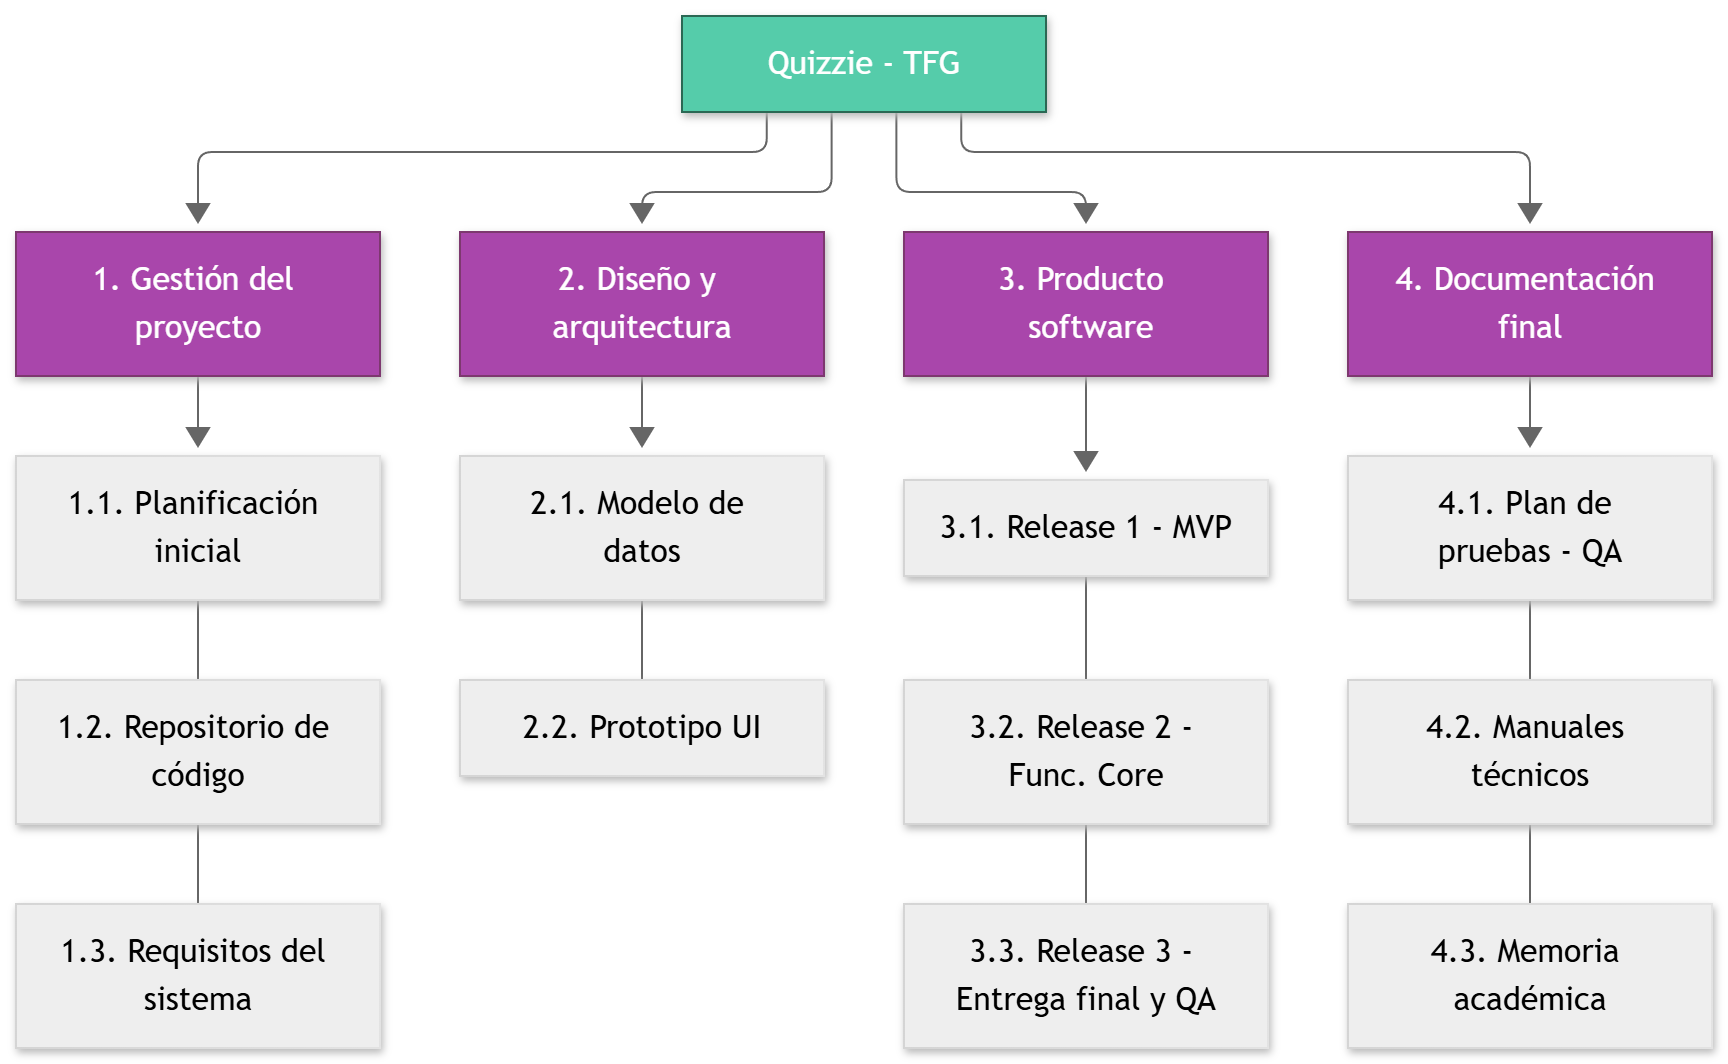
\includegraphics[width=0.87\textwidth]{figures/edt.png}
\caption{Estructura de Desglose del Trabajo (EDT).}
\label{fig:edt_grafica}
\end{figure}

Esta representación jerárquica descompone el proyecto en \textbf{paquetes de trabajo} y \textbf{entregables específicos} según las directrices de descomposición del estándar ISO/IEC/IEEE 21839 \cite{iso21839}, los cuales se detallan en el diccionario de la EDT.

\subsection{Diccionario de la EDT}\label{subsec:diccionario_edt}

El diccionario de la EDT define formalmente el \textbf{alcance} de cada entregable y desglosa las actividades necesarias para su consecución, especificando los perfiles profesionales asignados y la estimación temporal.

\subsubsection*{Paquete 1: Gestión del proyecto}
\addcontentsline{toc}{subsubsection}{Paquete 1: Gestión del proyecto}

\begin{table}[H]
\centering
\small
\renewcommand{\arraystretch}{1.2}
\makebox[\textwidth][c]{%
\begin{tabular}{P{3.3cm} P{5.8cm} @{}c@{}}
\bighline
\textbf{Entregable} & \textbf{Descripción} & 
\begin{tabular}{c c c}
  \makebox[2.2cm][c]{\textbf{Actividad}} & \makebox[2.3cm][c]{\textbf{Recurso}} & \makebox[1.2cm][c]{\textbf{Horas}}
\end{tabular} \\ \bighline

1.1. Planificación inicial & 
Acta de constitución del proyecto y cronograma base estimado para fijar los hitos académicos. & 
{%
  \renewcommand{\arraystretch}{1.2}
  \begin{tabular}[t]{>{\centering\arraybackslash}p{2.2cm} >{\centering\arraybackslash}p{2.3cm} >{\centering\arraybackslash}p{1.2cm}}
    \hyperref[act:01]{\textbf{ACT-01}} & Project Manager & 4h \\ \cmidrule(l{4pt}){1-3}
    \hyperref[act:02]{\textbf{ACT-02}} & Project Manager & 4h
  \end{tabular}%
} \\ \hline

1.2. Repositorio de código & 
Configuración de GitHub con reglas de protección de ramas, flujos de trabajo basados en fusiones (\textit{merges}) y plantillas estandarizadas para \textit{issues}. & 
{%
  \renewcommand{\arraystretch}{1.2}
  \begin{tabular}[t]{>{\centering\arraybackslash}p{2.2cm} >{\centering\arraybackslash}p{2.3cm} >{\centering\arraybackslash}p{1.2cm}}
    \hyperref[act:13]{\textbf{ACT-13}} & Técnico & 11h \\ \cmidrule(l{4pt}){1-3}
    \hyperref[act:14]{\textbf{ACT-14}} & Técnico & 5h \\ \cmidrule(l{4pt}){1-3}
    \hyperref[act:15]{\textbf{ACT-15}} & Técnico & 12h
  \end{tabular}%
} \\ \hline

1.3. Requisitos del sistema & 
Catálogo de requisitos funcionales y no funcionales, junto al modelado de casos de uso y flujos \textit{core} de la aplicación. & 
{%
  \renewcommand{\arraystretch}{1.2}
  \begin{tabular}[t]{>{\centering\arraybackslash}p{2.2cm} >{\centering\arraybackslash}p{2.3cm} >{\centering\arraybackslash}p{1.2cm}}
    \hyperref[act:08]{\textbf{ACT-08}} & Analista & 3h \\ \cmidrule(l{4pt}){1-3}
    \hyperref[act:09]{\textbf{ACT-09}} & Analista & 4h
  \end{tabular}%
} \\ \bighline
\end{tabular}%
}
\caption{Diccionario de la EDT - 1. Gestión del proyecto}
\label{tab:diccionario_edt_gestion_proyecto}
\end{table}

\subsubsection*{Paquete 2: Diseño y arquitectura}
\addcontentsline{toc}{subsubsection}{Paquete 2: Diseño y arquitectura}

\begin{table}[H]
\centering
\small
\renewcommand{\arraystretch}{1.2}
\makebox[\textwidth][c]{%
\begin{tabular}{P{3.3cm} P{5.8cm} @{}c@{}}
\bighline
\textbf{Entregable} & \textbf{Descripción} & 
\begin{tabular}{c c c}
  \makebox[2.2cm][c]{\textbf{Actividad}} & \makebox[2.3cm][c]{\textbf{Recurso}} & \makebox[1.2cm][c]{\textbf{Horas}}
\end{tabular} \\ \bighline

2.1. Modelo de datos & 
Diseño conceptual, lógico y físico de la base de datos relacional, materializado en el diagrama de entidades del sistema. & 
{%
  \renewcommand{\arraystretch}{1.2}
  \begin{tabular}[t]{>{\centering\arraybackslash}p{2.2cm} >{\centering\arraybackslash}p{2.3cm} >{\centering\arraybackslash}p{1.2cm}}
    \hyperref[act:10]{\textbf{ACT-10}} & Analista & 4h \\ \cmidrule(l{4pt}){1-3}
    \hyperref[act:11]{\textbf{ACT-11}} & Analista & 4h \\ \cmidrule(l{4pt}){1-3}
    \hyperref[act:12]{\textbf{ACT-12}} & Programador Backend & 2h
  \end{tabular}%
} \\ \hline

2.2. Prototipo UI & 
Diseños visuales y plantillas para las pantallas del sistema. & 
{%
  \renewcommand{\arraystretch}{1.2}
  \begin{tabular}[t]{>{\centering\arraybackslash}p{2.2cm} >{\centering\arraybackslash}p{2.3cm} >{\centering\arraybackslash}p{1.2cm}}
    \hyperref[act:03]{\textbf{ACT-03}} & Diseñador UI & 2h \\ \cmidrule(l{4pt}){1-3}
    \hyperref[act:04]{\textbf{ACT-04}} & Diseñador UI & 5h \\ \cmidrule(l{4pt}){1-3}
    \hyperref[act:05]{\textbf{ACT-05}} & Diseñador UI & 5h
  \end{tabular}%
} \\ \bighline
\end{tabular}%
}
\caption{Diccionario de la EDT - 2. Diseño y arquitectura}
\label{tab:diccionario_edt_diseno_arquitectura}
\end{table}

\subsubsection*{Paquete 3: Producto software}
\addcontentsline{toc}{subsubsection}{Paquete 3: Producto software}

\begin{table}[H]
\centering
\small
\renewcommand{\arraystretch}{1.2}
\makebox[\textwidth][c]{%
\begin{tabular}{P{3.3cm} P{5.8cm} @{}c@{}}
\bighline
\textbf{Entregable} & \textbf{Descripción} & 
\begin{tabular}{c c c}
  \makebox[2.2cm][c]{\textbf{Actividad}} & \makebox[2.3cm][c]{\textbf{Recurso}} & \makebox[1.2cm][c]{\textbf{Horas}}
\end{tabular} \\ \bighline

3.1. Release 1 (MVP) & 
Habilitación y despliegue del flujo completo base del sistema, permitiendo la creación de cuestionarios por parte del profesor y la realización de los mismos por los alumnos. & 
{%
  \renewcommand{\arraystretch}{1.2}
  \begin{tabular}[t]{>{\centering\arraybackslash}p{2.2cm} >{\centering\arraybackslash}p{2.3cm} >{\centering\arraybackslash}p{1.2cm}}
    \hyperref[act:16]{\textbf{ACT-16}} & Programador Backend & 25h \\ \cmidrule(l{4pt}){1-3}
    \hyperref[act:17]{\textbf{ACT-17}} & Programador Frontend & 25h \\ \cmidrule(l{4pt}){1-3}
    \hyperref[act:18]{\textbf{ACT-18}} & Programador Backend & 15h
  \end{tabular}%
} \\ \hline

3.2. Release 2 (Funcionalidades Core) & 
Implementación de la capa de comunicación en tiempo real mediante WebSockets y el motor de validación de datos del sistema. & 
{%
  \renewcommand{\arraystretch}{1.2}
  \begin{tabular}[t]{>{\centering\arraybackslash}p{2.2cm} >{\centering\arraybackslash}p{2.3cm} >{\centering\arraybackslash}p{1.2cm}}
    \hyperref[act:21]{\textbf{ACT-21}} & Programador Backend & 20h \\ \cmidrule(l{4pt}){1-3}
    \hyperref[act:22]{\textbf{ACT-22}} & Programador Frontend & 17h \\ \cmidrule(l{4pt}){1-3}
    \hyperref[act:23]{\textbf{ACT-23}} & Programador Backend & 12h
  \end{tabular}%
} \\ \hline

3.3. Release 3 (Entrega final y QA) & 
Integración de funcionalidades avanzadas de gestión, pulido general de la interfaz y despliegue del sistema. & 
{%
  \renewcommand{\arraystretch}{1.2}
  \begin{tabular}[t]{>{\centering\arraybackslash}p{2.2cm} >{\centering\arraybackslash}p{2.3cm} >{\centering\arraybackslash}p{1.2cm}}
    \hyperref[act:24]{\textbf{ACT-24}} & Programador Backend & 5h \\ \cmidrule(l{4pt}){1-3}
    \hyperref[act:25]{\textbf{ACT-25}} & Programador Frontend & 5h \\ \cmidrule(l{4pt}){1-3}
    \hyperref[act:26]{\textbf{ACT-26}} & Técnico & 3h
  \end{tabular}%
} \\ \bighline
\end{tabular}%
}
\caption{Diccionario de la EDT - 3. Producto software}
\label{tab:diccionario_edt_producto_software}
\end{table}

\subsubsection*{Paquete 4: Documentación final}
\addcontentsline{toc}{subsubsection}{Paquete 4: Documentación final}

\begin{table}[H]
\centering
\small
\renewcommand{\arraystretch}{1.2}
\makebox[\textwidth][c]{%
\begin{tabular}{P{3.3cm} P{5.8cm} @{}c@{}}
\bighline
\textbf{Entregable} & \textbf{Descripción} & 
\begin{tabular}{c c c}
  \makebox[2.2cm][c]{\textbf{Actividad}} & \makebox[2.3cm][c]{\textbf{Recurso}} & \makebox[1.2cm][c]{\textbf{Horas}}
\end{tabular} \\ \bighline

4.1. Plan de pruebas (QA) & 
Diseño y ejecución de baterías de test de integración y \textit{scripts} específicos de pruebas de carga. & 
{%
  \renewcommand{\arraystretch}{1.2}
  \begin{tabular}[t]{>{\centering\arraybackslash}p{2.2cm} >{\centering\arraybackslash}p{2.3cm} >{\centering\arraybackslash}p{1.2cm}}
    \hyperref[act:19]{\textbf{ACT-19}} & Tester & 7h \\ \cmidrule(l{4pt}){1-3}
    \hyperref[act:20]{\textbf{ACT-20}} & Tester & 8h
  \end{tabular}%
} \\ \hline

4.2. Manuales técnicos & 
Redacción del manual de usuario y del manual de despliegue. & 
{%
  \renewcommand{\arraystretch}{1.2}
  \begin{tabular}[t]{>{\centering\arraybackslash}p{2.2cm} >{\centering\arraybackslash}p{2.3cm} >{\centering\arraybackslash}p{1.2cm}}
    \hyperref[act:06]{\textbf{ACT-06}} & Analista & 2h \\ \cmidrule(l{4pt}){1-3}
    \hyperref[act:07]{\textbf{ACT-07}} & Técnico & 1h
  \end{tabular}%
} \\ \hline

4.3. Memoria académica & 
Redacción técnica, maquetación y consolidación del documento final del TFG junto con el diseño de las diapositivas para la defensa. & 
{%
  \renewcommand{\arraystretch}{1.2}
  \begin{tabular}[t]{>{\centering\arraybackslash}p{2.2cm} >{\centering\arraybackslash}p{2.3cm} >{\centering\arraybackslash}p{1.2cm}}
    \hyperref[act:27]{\textbf{ACT-27}} & Analista & 70h \\ \cmidrule(l{4pt}){1-3}
    \hyperref[act:28]{\textbf{ACT-28}} & Diseñador UI & 10h \\ \cmidrule(l{4pt}){1-3}
    \hyperref[act:29]{\textbf{ACT-29}} & Project Manager & 10h
  \end{tabular}%
} \\ \bighline
\end{tabular}%
}
\caption{Diccionario de la EDT - 4. Documentación final}
\label{tab:diccionario_edt_documentacion_final}
\end{table}


\section{Línea base del cronograma}\label{sec:linea_base_del_cronograma}
A partir de los paquetes de trabajo de la \hyperref[subsec:edt]{EDT}, se ha planificado la distribución temporal del proyecto. El flujo de trabajo se estructura dividiendo el ciclo de vida en fases temporales que agrupan las actividades y culminan en hitos de control.

\subsection{Fases del proyecto}\label{sub:fases_del_proyecto}

El proyecto se divide en 10 fases temporales consecutivas y paralelas, que se han organizado en 4 bloques de trabajo fundamentales:

\begin{table}[H]
\centering
\small
\renewcommand{\arraystretch}{1.4}
\makebox[\textwidth][c]{%
\begin{tabularx}{1\textwidth}{llYl}
\bighline
\textbf{ID} &  \textbf{Nombre} & \textbf{Descripción} & \textbf{Bloque} \\ \bighline
F-01 & Planificación & Planificación inicial, estimación de tiempos y recursos. & Gestión y planificación \\ \hline
F-02 & Documentación & Redacción de manuales y documentación técnica de soporte. & Documentación y cierre \\ \hline
F-03 & Inicio & Configuración del entorno base y análisis de requisitos. & Gestión y planificación \\ \hline
F-04 & CI/CD & Automatización de flujos de trabajo e integración continua. & Ciclo de vida y calidad \\ \hline
F-05 \label{fase:mvp} & MVP & Construcción de la primera versión mínima funcional. & Desarrollo de código \\ \hline
F-06 & Testing & Diseño y ejecución de la batería de pruebas del sistema. & Ciclo de vida y calidad \\ \hline
F-07 \label{fase:core} & Core & Desarrollo de las características principales (WebSockets). & Desarrollo de código \\ \hline
F-08 \label{fase:qa} & QA & Estabilización de código y corrección de errores finales. & Desarrollo de código \\ \hline
F-09 & Memoria & Consolidación, revisión final y entrega de la memoria. & Documentación y cierre \\ \hline
F-10 & Defensa & Preparación del material de soporte y ensayos. & Documentación y cierre \\ \bighline
\end{tabularx}%
}
\caption{Fases temporales del proyecto.}
\label{tab:fases}
\end{table}

\subsection{Lista de actividades}\label{sub:lista_de_actividades}

Cada una de las actividades del cronograma conserva una relación directa con los paquetes de trabajo definidos en el diccionario de la EDT. Para garantizar el seguimiento y la trazabilidad temporal, a continuación se detallan todas las tareas del proyecto:

\begin{table}[H]
\centering
\small
\renewcommand{\arraystretch}{1.48}
\makebox[\textwidth][c]{%
\begin{tabularx}{1.1\textwidth}{llY}
\bighline
\textbf{Fase} & \textbf{ID} & \textbf{Actividad} \\ \bighline

F-01 -- Planificación & ACT-01\label{act:01} & Redacción del acta de constitución \\ \cline{2-3}
& ACT-02\label{act:02} & Definición de hitos y estimación del cronograma inicial \\ \cline{2-3}
& ACT-03\label{act:03} & Elección de estilos, paleta de colores y componentes básicos \\ \cline{2-3}
& ACT-04\label{act:04} & Diseño de prototipos de las pantallas de gestión del profesor \\ \cline{2-3}
& ACT-05\label{act:05} & Diseño de la interfaz de respuesta para pantallas de alumnos \\ \hline

F-02 -- Documentación & ACT-06\label{act:06} & Elaboración del manual funcional como guía para usuarios \\ \cline{2-3}
& ACT-07\label{act:07} & Redacción del manual de despliegue técnico de infraestructura \\ \cline{2-3}
& ACT-08\label{act:08} & Elicitación y redacción de requisitos funcionales y no funcionales \\ \cline{2-3}
& ACT-09\label{act:09} & Modelado de diagramas de casos de uso y flujos esenciales \\ \cline{2-3}
& ACT-10\label{act:10} & Diseño del modelo conceptual y lógico de datos \\ \cline{2-3}
& ACT-11\label{act:11} & Modelado del diagrama de entidades relacional \\ \cline{2-3}
& ACT-12\label{act:12} & Generación del \textit{script} de inicialización de tablas y poblado \\ \hline

F-03 -- Inicio & ACT-13\label{act:13} & Inicialización del repositorio en GitHub y estructura base \\ \hline

F-04 -- CI/CD & ACT-14\label{act:14} & Diseño de \textit{templates} para \textit{issues} y automatización base \\ \cline{2-3}
& ACT-15\label{act:15} & Desarrollo de \textit{scripts} de despliegue e integración continuos \\ \hline

F-05 -- MVP & ACT-16\label{act:16} & Diseño y desarrollo de la persistencia base para cuestionarios \\ \cline{2-3}
& ACT-17\label{act:17} & Implementación de la interfaz de creación de tests y panel base \\ \cline{2-3}
& ACT-18\label{act:18} & Lógica de control y validación para la ejecución asíncrona \\ \hline

F-06 -- Testing & ACT-19\label{act:19} & Desarrollo y ejecución de test de integración de servicios \\ \cline{2-3}
& ACT-20\label{act:20} & Pruebas de componentes, de carga y \textit{end-to-end} \\ \hline

F-07 -- Core & ACT-21\label{act:21} & Desarrollo de la infraestructura síncrona y canales WebSocket \\ \cline{2-3}
& ACT-22\label{act:22} & Implementación en frontend de la conexión reactiva a salas \\ \cline{2-3}
& ACT-23\label{act:23} & Programación del motor de validación y control de integridad \\ \hline

F-08 -- QA & ACT-24\label{act:24} & Implementación del módulo de autenticación y panel avanzado \\ \cline{2-3}
& ACT-25\label{act:25} & Desarrollo de vistas de historial y exportación de datos \\ \cline{2-3}
& ACT-26\label{act:26} & Puesta a punto, empaquetado, corrección de errores y despliegue \\ \hline

F-09 -- Memoria & ACT-27\label{act:27} & Redacción y estructuración técnica de la memoria en LaTeX \\ \hline

F-10 -- Defensa & ACT-28\label{act:28} & Diseño, desarrollo y maquetación de diapositivas de defensa \\ \cline{2-3}
& ACT-29\label{act:29} & Ensayos de oratoria y preparación de la defensa pública \\ \bighline
\end{tabularx}%
}
\caption{Actividades organizadas por su fase del cronograma.}
\label{tab:lista_actividades}
\end{table}

\subsection{Lista de hitos}\label{sub:lista_de_hitos}

Los hitos representan los puntos de control clave y logros de duración cero dentro del cronograma del proyecto. Su consecución suponen grandes avances en el desarrollo o la finalización de fases completas, y permiten evaluar el progreso general del proyecto. 

\begin{table}[H]
\centering
\small
\renewcommand{\arraystretch}{1.6}
\makebox[\textwidth][c]{%
\begin{tabularx}{1\textwidth}{llYc}
\bighline
\textbf{Fase} & \textbf{ID} & \textbf{Hito / logro} & \textbf{Límite} \\ \bighline

F-01 -- Planificación & H-01 & Acta de constitución del proyecto redactada y firmada & 21 Ene \\ \cline{2-4}
& H-02 & Líneas base del proyecto constituidas y aprobadas & 28 Ene \\ \hline

F-02 -- Documentación & H-03 & Catálogo de requisitos, casos de uso y modelos de datos definidos & 18 Feb \\ \cline{2-4}
& H-04 & Manuales técnicos de usuario y despliegue finalizados & 14 Abr \\ \hline

F-03 -- Inicio & H-05 & Repositorio inicializado y entorno de desarrollo listo & 11 Feb \\ \hline

F-04 -- CI/CD & H-06 & Flujo de CI/CD automatizado y plantillas de trabajo desplegadas & 1 Mar \\ \hline

F-05 -- MVP & H-07 & Funcionalidades del MVP operativas (creación y respuesta de tests) & 8 Mar \\ \hline

F-06 -- Testing & H-08 & Baterías de pruebas de software ejecutadas y superadas con éxito & 26 Abr \\ \hline

F-07 -- Core & H-09 & Conexión y respuesta a cuestionarios en tiempo real operativos & 29 Mar \\ \cline{2-4}
& H-10 & Motor de validación y control de integridad de respuestas completado & 12 Abr \\ \hline

F-08 -- QA & H-11 & Vistas de historial de salas pasadas y exportación de datos funcionales & 24 Abr \\ \hline

F-09 -- Memoria & H-12 & Memoria académica consolidada y entregada & 17 May \\ \hline

F-10 -- Defensa & H-13 & Presentación y material de soporte maquetados para la defensa & 5 Jun \\ \cline{2-4}
& H-14 & Defensa pública del proyecto ejecutada ante el tribunal & 10 Jun \\ \bighline
\end{tabularx}%
}
\caption{Hitos de control del proyecto.}
\label{tab:lista_hitos}
\end{table}


\subsection{Diagrama de Gantt}\label{sub:diagrama_de_gantt}
El siguiente diagrama de Gantt\cite{wilson2003gantt} sintetiza de manera visual la distribución cronológica del proyecto, clave para el seguimiento del trabajo realizado y asegurar el cumplimiento de los plazos fijados.

\begin{figure}[H]
\centering
\makebox[\textwidth][c]{
\begin{ganttchart}[
    hgrid=false, 
    vgrid=false, 
    x unit=0.115cm,
    y unit title=0.65cm, 
    y unit chart=0.95cm, 
    bar height=0.55,
    time slot format=isodate,
    inline,
    bar label font=\small\bfseries\color{white},
    ganttbar label node/.style={text width=0pt, inner sep=0pt},
    title label font=\small\bfseries,
    title calendar link/.style={draw=black},
    canvas/.style={draw=black, fill=white}
]{2026-01-15}{2026-06-12}

    % Única fila de meses
    \gantttitle{Ene}{17}
    \gantttitle{Feb}{28}
    \gantttitle{Mar}{31}
    \gantttitle{Abr}{30}
    \gantttitle{May}{31}
    \gantttitle{Jun}{12} \\

    % Fases
    \ganttbar[bar/.style={fill=primaryMagenta, draw=primaryMagenta, rounded corners=2.5pt}]{F01-Plan}{2026-01-15}{2026-01-28} \\
    \ganttbar[bar/.style={fill=secondaryMagenta, draw=secondaryMagenta, rounded corners=2.5pt}]{F02-Documentación}{2026-01-29}{2026-04-14} \\
    \ganttbar[bar/.style={fill=primaryMagenta, draw=primaryMagenta, rounded corners=2.5pt}]{F03-Inicio}{2026-01-29}{2026-02-11} \\
    \ganttbar[bar/.style={fill=secondaryCyan, draw=secondaryCyan, rounded corners=2.5pt}]{F04-CI/CD}{2026-02-12}{2026-04-26} \\
    \ganttbar[bar/.style={fill=primaryCyan, draw=primaryCyan, rounded corners=2.5pt}]{F05-MVP}{2026-02-19}{2026-03-08} \\
    \ganttbar[bar/.style={fill=secondaryCyan, draw=secondaryCyan, rounded corners=2.5pt}]{F06-Testing}{2026-02-24}{2026-04-26} \\
    \ganttbar[bar/.style={fill=primaryCyan, draw=primaryCyan, rounded corners=2.5pt}]{F07-Core}{2026-03-09}{2026-04-12} \\
    \ganttbar[bar/.style={fill=primaryCyan, draw=primaryCyan, rounded corners=2.5pt}]{F08-QA}{2026-04-13}{2026-04-24} \\
    \ganttbar[bar/.style={fill=secondaryMagenta, draw=secondaryMagenta, rounded corners=2.5pt}]{F09-Memoria}{2026-04-15}{2026-05-17} \\
    \ganttbar[bar/.style={fill=secondaryMagenta, draw=secondaryMagenta, rounded corners=2.5pt}]{F10-Defensa}{2026-05-18}{2026-06-12} \\
    % Espacio inferior para holgura de hitos
    \ganttbar[bar/.style={draw=none, fill=none}]{}{2026-01-15}{2026-01-15}

    \begin{pgfonlayer}{behind}
        
        % 1.1 Líneas semanales 
        \ganttvrule[vrule/.style={draw=gray!70, densely dotted, thick}]{}{2026-01-19}
        \ganttvrule[vrule/.style={draw=gray!70, densely dotted, thick}]{}{2026-01-26}
        \ganttvrule[vrule/.style={draw=gray!70, densely dotted, thick}]{}{2026-02-02}
        \ganttvrule[vrule/.style={draw=gray!70, densely dotted, thick}]{}{2026-02-09}
        \ganttvrule[vrule/.style={draw=gray!70, densely dotted, thick}]{}{2026-02-16}
        \ganttvrule[vrule/.style={draw=gray!70, densely dotted, thick}]{}{2026-02-23}
        \ganttvrule[vrule/.style={draw=gray!70, densely dotted, thick}]{}{2026-03-02}
        \ganttvrule[vrule/.style={draw=gray!70, densely dotted, thick}]{}{2026-03-09}
        \ganttvrule[vrule/.style={draw=gray!70, densely dotted, thick}]{}{2026-03-16}
        \ganttvrule[vrule/.style={draw=gray!70, densely dotted, thick}]{}{2026-03-23}
        \ganttvrule[vrule/.style={draw=gray!70, densely dotted, thick}]{}{2026-03-30}
        \ganttvrule[vrule/.style={draw=gray!70, densely dotted, thick}]{}{2026-04-06}
        \ganttvrule[vrule/.style={draw=gray!70, densely dotted, thick}]{}{2026-04-13}
        \ganttvrule[vrule/.style={draw=gray!70, densely dotted, thick}]{}{2026-04-20}
        \ganttvrule[vrule/.style={draw=gray!70, densely dotted, thick}]{}{2026-04-27}
        \ganttvrule[vrule/.style={draw=gray!70, densely dotted, thick}]{}{2026-05-04}
        \ganttvrule[vrule/.style={draw=gray!70, densely dotted, thick}]{}{2026-05-11}
        \ganttvrule[vrule/.style={draw=gray!70, densely dotted, thick}]{}{2026-05-18}
        \ganttvrule[vrule/.style={draw=gray!70, densely dotted, thick}]{}{2026-05-25}
        \ganttvrule[vrule/.style={draw=gray!70, densely dotted, thick}]{}{2026-06-01}
        \ganttvrule[vrule/.style={draw=gray!70, densely dotted, thick}]{}{2026-06-08}

        % 1.2 Líneas verticales discontinuas de los hitos
        \ganttvrule[vrule/.style={draw=primaryMagenta, dashed, line width=1.3pt}]{}{2026-01-21}
        \ganttvrule[vrule/.style={draw=primaryMagenta, dashed, line width=1.3pt}]{}{2026-01-28}
        \ganttvrule[vrule/.style={draw=primaryMagenta, dashed, line width=1.3pt}]{}{2026-02-11}
        \ganttvrule[vrule/.style={draw=primaryCyan, dashed, line width=1.3pt}]{}{2026-03-08}
        \ganttvrule[vrule/.style={draw=primaryCyan, dashed, line width=1.3pt}]{}{2026-03-29}
        \ganttvrule[vrule/.style={draw=primaryCyan, dashed, line width=1.3pt}]{}{2026-04-12}
        \ganttvrule[vrule/.style={draw=primaryCyan, dashed, line width=1.3pt}]{}{2026-04-24}
        \ganttvrule[vrule/.style={draw=secondaryCyan, dashed, line width=1.3pt}]{}{2026-03-01}
        \ganttvrule[vrule/.style={draw=secondaryCyan, dashed, line width=1.3pt}]{}{2026-04-26}
        \ganttvrule[vrule/.style={draw=secondaryMagenta, dashed, line width=1.3pt}]{}{2026-02-18}
        \ganttvrule[vrule/.style={draw=secondaryMagenta, dashed, line width=1.3pt}]{}{2026-04-14}
        \ganttvrule[vrule/.style={draw=secondaryMagenta, dashed, line width=1.3pt}]{}{2026-05-17}
        \ganttvrule[vrule/.style={draw=secondaryMagenta, dashed, line width=1.3pt}]{}{2026-06-05}
        \ganttvrule[vrule/.style={draw=secondaryMagenta, dashed, line width=1.3pt}]{}{2026-06-10}

    
        % 2.1 Números semanales superiores con fondo blanco
        \ganttvrule[vrule/.style={draw=none}, vrule label node/.style={at end, anchor=north, yshift=305pt, font=\small\bfseries\color{gray!90!black}, fill=white, inner sep=2pt, rounded corners=1pt}]{19}{2026-01-19}
        \ganttvrule[vrule/.style={draw=none}, vrule label node/.style={at end, anchor=north, yshift=305pt, font=\small\bfseries\color{gray!90!black}, fill=white, inner sep=2pt, rounded corners=1pt}]{26}{2026-01-26}
        \ganttvrule[vrule/.style={draw=none}, vrule label node/.style={at end, anchor=north, yshift=305pt, font=\small\bfseries\color{gray!90!black}, fill=white, inner sep=2pt, rounded corners=1pt}]{02}{2026-02-02}
        \ganttvrule[vrule/.style={draw=none}, vrule label node/.style={at end, anchor=north, yshift=305pt, font=\small\bfseries\color{gray!90!black}, fill=white, inner sep=2pt, rounded corners=1pt}]{09}{2026-02-09}
        \ganttvrule[vrule/.style={draw=none}, vrule label node/.style={at end, anchor=north, yshift=305pt, font=\small\bfseries\color{gray!90!black}, fill=white, inner sep=2pt, rounded corners=1pt}]{16}{2026-02-16}
        \ganttvrule[vrule/.style={draw=none}, vrule label node/.style={at end, anchor=north, yshift=305pt, font=\small\bfseries\color{gray!90!black}, fill=white, inner sep=2pt, rounded corners=1pt}]{23}{2026-02-23}
        \ganttvrule[vrule/.style={draw=none}, vrule label node/.style={at end, anchor=north, yshift=305pt, font=\small\bfseries\color{gray!90!black}, fill=white, inner sep=2pt, rounded corners=1pt}]{02}{2026-03-02}
        \ganttvrule[vrule/.style={draw=none}, vrule label node/.style={at end, anchor=north, yshift=305pt, font=\small\bfseries\color{gray!90!black}, fill=white, inner sep=2pt, rounded corners=1pt}]{09}{2026-03-09}
        \ganttvrule[vrule/.style={draw=none}, vrule label node/.style={at end, anchor=north, yshift=305pt, font=\small\bfseries\color{gray!90!black}, fill=white, inner sep=2pt, rounded corners=1pt}]{16}{2026-03-16}
        \ganttvrule[vrule/.style={draw=none}, vrule label node/.style={at end, anchor=north, yshift=305pt, font=\small\bfseries\color{gray!90!black}, fill=white, inner sep=2pt, rounded corners=1pt}]{23}{2026-03-23}
        \ganttvrule[vrule/.style={draw=none}, vrule label node/.style={at end, anchor=north, yshift=305pt, font=\small\bfseries\color{gray!90!black}, fill=white, inner sep=2pt, rounded corners=1pt}]{30}{2026-03-30}
        \ganttvrule[vrule/.style={draw=none}, vrule label node/.style={at end, anchor=north, yshift=305pt, font=\small\bfseries\color{gray!90!black}, fill=white, inner sep=2pt, rounded corners=1pt}]{06}{2026-04-06}
        \ganttvrule[vrule/.style={draw=none}, vrule label node/.style={at end, anchor=north, yshift=305pt, font=\small\bfseries\color{gray!90!black}, fill=white, inner sep=2pt, rounded corners=1pt}]{13}{2026-04-13}
        \ganttvrule[vrule/.style={draw=none}, vrule label node/.style={at end, anchor=north, yshift=305pt, font=\small\bfseries\color{gray!90!black}, fill=white, inner sep=2pt, rounded corners=1pt}]{20}{2026-04-20}
        \ganttvrule[vrule/.style={draw=none}, vrule label node/.style={at end, anchor=north, yshift=305pt, font=\small\bfseries\color{gray!90!black}, fill=white, inner sep=2pt, rounded corners=1pt}]{27}{2026-04-27}
        \ganttvrule[vrule/.style={draw=none}, vrule label node/.style={at end, anchor=north, yshift=305pt, font=\small\bfseries\color{gray!90!black}, fill=white, inner sep=2pt, rounded corners=1pt}]{04}{2026-05-04}
        \ganttvrule[vrule/.style={draw=none}, vrule label node/.style={at end, anchor=north, yshift=305pt, font=\small\bfseries\color{gray!90!black}, fill=white, inner sep=2pt, rounded corners=1pt}]{11}{2026-05-11}
        \ganttvrule[vrule/.style={draw=none}, vrule label node/.style={at end, anchor=north, yshift=305pt, font=\small\bfseries\color{gray!90!black}, fill=white, inner sep=2pt, rounded corners=1pt}]{18}{2026-05-18}
        \ganttvrule[vrule/.style={draw=none}, vrule label node/.style={at end, anchor=north, yshift=305pt, font=\small\bfseries\color{gray!90!black}, fill=white, inner sep=2pt, rounded corners=1pt}]{25}{2026-05-25}
        \ganttvrule[vrule/.style={draw=none}, vrule label node/.style={at end, anchor=north, yshift=305pt, font=\small\bfseries\color{gray!90!black}, fill=white, inner sep=2pt, rounded corners=1pt}]{01}{2026-06-01}
        \ganttvrule[vrule/.style={draw=none}, vrule label node/.style={at end, anchor=north, yshift=305pt, font=\small\bfseries\color{gray!90!black}, fill=white, inner sep=2pt, rounded corners=1pt}]{08}{2026-06-08}

        % 2.2 Etiquetas de hitos 
        % Gestión y planificación
        \ganttvrule[vrule/.style={draw=none}, vrule label node/.style={anchor=south, yshift=4pt, font=\small\bfseries\color{primaryMagenta}, fill=white, inner sep=2pt, rounded corners=1pt}]{H-01}{2026-01-21}
        \ganttvrule[vrule/.style={draw=none}, vrule label node/.style={anchor=south, yshift=0.55cm, font=\small\bfseries\color{primaryMagenta}, fill=white, inner sep=2pt, rounded corners=1pt}]{H-02}{2026-01-28}
        \ganttvrule[vrule/.style={draw=none}, vrule label node/.style={anchor=south, yshift=4pt, font=\small\bfseries\color{primaryMagenta}, fill=white, inner sep=2pt, rounded corners=1pt}]{H-05}{2026-02-11}

        % Desarrollo de código
        \ganttvrule[vrule/.style={draw=none}, vrule label node/.style={anchor=south, yshift=0.55cm, font=\small\bfseries\color{primaryCyan}, fill=white, inner sep=2pt, rounded corners=1pt}]{H-07}{2026-03-08}
        \ganttvrule[vrule/.style={draw=none}, vrule label node/.style={anchor=south, yshift=4pt, font=\small\bfseries\color{primaryCyan}, fill=white, inner sep=2pt, rounded corners=1pt}]{H-09}{2026-03-29}
        \ganttvrule[vrule/.style={draw=none}, vrule label node/.style={anchor=south, yshift=4pt, font=\small\bfseries\color{primaryCyan}, fill=white, inner sep=2pt, rounded corners=1pt}]{H-10}{2026-04-12}
        \ganttvrule[vrule/.style={draw=none}, vrule label node/.style={anchor=south, yshift=4pt, font=\small\bfseries\color{primaryCyan}, fill=white, inner sep=2pt, rounded corners=1pt}]{H-11}{2026-04-24}

        % Ciclo de vida y calidad
        \ganttvrule[vrule/.style={draw=none}, vrule label node/.style={anchor=south, yshift=4pt, font=\small\bfseries\color{secondaryCyan}, fill=white, inner sep=2pt, rounded corners=1pt}]{H-06}{2026-03-01}
        \ganttvrule[vrule/.style={draw=none}, vrule label node/.style={anchor=south, yshift=0.55cm, font=\small\bfseries\color{secondaryCyan}, fill=white, inner sep=2pt, rounded corners=1pt}]{H-08}{2026-04-26}

        % Documentación y cierre
        \ganttvrule[vrule/.style={draw=none}, vrule label node/.style={anchor=south, yshift=0.55cm, font=\small\bfseries\color{secondaryMagenta}, fill=white, inner sep=2pt, rounded corners=1pt}]{H-03}{2026-02-18}
        \ganttvrule[vrule/.style={draw=none}, vrule label node/.style={anchor=south, yshift=0.55cm, font=\small\bfseries\color{secondaryMagenta}, fill=white, inner sep=2pt, rounded corners=1pt}]{H-04}{2026-04-14}
        \ganttvrule[vrule/.style={draw=none}, vrule label node/.style={anchor=south, yshift=4pt, font=\small\bfseries\color{secondaryMagenta}, fill=white, inner sep=2pt, rounded corners=1pt}]{H-12}{2026-05-17}
        \ganttvrule[vrule/.style={draw=none}, vrule label node/.style={anchor=south, yshift=0.55cm, font=\small\bfseries\color{secondaryMagenta}, fill=white, inner sep=2pt, rounded corners=1pt}]{H-13}{2026-06-05}
        \ganttvrule[vrule/.style={draw=none}, vrule label node/.style={anchor=south, yshift=4pt, font=\small\bfseries\color{secondaryMagenta}, fill=white, inner sep=2pt, rounded corners=1pt}]{H-14}{2026-06-10}
    \end{pgfonlayer}

\end{ganttchart}
}
\vspace{0.25cm}
\begin{center}
\small
\begin{tabular}{clccl}
\fcolorbox{black}{primaryMagenta}{\rule{0pt}{4pt}\rule{4pt}{0pt}} & Gestión y planificación & \hspace{0.5cm} &
\fcolorbox{black}{primaryCyan}{\rule{0pt}{4pt}\rule{4pt}{0pt}} & Desarrollo de código \\
\fcolorbox{black}{secondaryCyan}{\rule{0pt}{4pt}\rule{4pt}{0pt}} & Ciclo de vida y calidad & \hspace{0.5cm} &
\fcolorbox{black}{secondaryMagenta}{\rule{0pt}{4pt}\rule{4pt}{0pt}} & Documentación y cierre
\end{tabular}
\end{center}
\caption{Diagrama de Gantt inicial del proyecto.}
\label{fig:gantt}
\end{figure}

\section{Línea base de Costes}\label{sec:linea_base_de_costes}
El desarrollo de un proyecto como \textit{Quizzie} no solo exige viabilidad técnica, sino también un \textbf{modelo financiero sostenible} que justifique su implantación frente a otras soluciones. Para ello, se analizan a continuación los costes operativos, el impacto económico que supone el escalado de la infraestructura y el Coste Total de Propiedad (TCO).

\subsection{Análisis de costes}\label{sub:analisis_de_costes}
El estudio económico de la plataforma se fundamenta en la clasificación financiera de costes de tecnologías de la información \cite{remenyi2007it}, dividiéndose en dos componentes esenciales: los Gastos de Capital (\textit{Capital Expenditure} o \textbf{CAPEX}), que engloban el coste de desarrollo y los recursos fijos iniciales, y los Gastos Operativos (\textit{Operational Expenditure} o \textbf{OPEX}), que representan el coste recurrente de la infraestructura en la nube para la explotación en producción.

\begin{table}[H]
\centering
\small
\renewcommand{\arraystretch}{1.4}
\makebox[\textwidth][c]{%
\begin{tabularx}{0.9\textwidth}{Yr}
\bighline
\textbf{Concepto} & \textbf{Coste neto} \\ \bighline
Costes laborales & 11.552,65 \euro \\ \hline
Equipamiento informático & 500,00 \euro \\ \hline
Licencia comercial anual Google AI Premium (Gemini Pro) & 218,07 \euro \\ \hline
Licencia GitHub Team (6 meses) & 21,82 \euro \\ \hline
Licencia Microsoft Teams Essentials (6 meses) & 21,82 \euro \\ \hline
Reserva de contingencia & 12.314,36 \euro \\ \bighline
\textbf{Total CAPEX} & \textbf{13.545,80 \euro} \\ \bighline
\end{tabularx}%
}
\caption{Resumen de Gastos de Capital (CAPEX).}
\label{tab:resumen_capex}
\end{table}

Para justificar el coste laboral del CAPEX, se adopta un \textbf{modelo de roles mixtos} debido a que el proyecto ha sido ejecutado íntegramente por un único ingeniero. De este modo, cada actividad de la EDT se presupuesta en función del perfil profesional específico requerido para su ejecución técnica.

Con el fin de garantizar el rigor y la objetividad de las tarifas aplicadas, los precios base por hora se han extraído del \textit{Informe Final sobre la Consulta Preliminar del Mercado: ``Perfiles Profesionales Ámbito Informático''} de la Junta de Andalucía \cite{juntaTIC2018}. Siguiendo las directrices de dicho organismo, se utiliza como referencia la \textbf{media acotada}, métrica estadística que descarta valores atípicos del sector mediante el test de Tukey.

Sobre la base salarial neta resultante de 8.886,65 \euro, se ha aplicado un \textbf{recargo del 30\%} en concepto de cotizaciones a la Seguridad Social y costes de contratación directos, consolidando el coste laboral real en \textbf{11.552,65 \euro}. El desglose detallado de horas y perfiles profesionales que sustenta este cálculo se recoge en la siguiente tabla de costes netos laborales.

\begin{table}[H]
\centering
\small
\renewcommand{\arraystretch}{1.2}
\makebox[\textwidth][c]{%
\begin{tabularx}{0.9\textwidth}{Ycccc}
\bighline
\textbf{Recurso (Rol)} & \textbf{Actividad} & \textbf{Precio/hora} & \textbf{Horas} & \textbf{Coste neto} \\ \bighline
\textbf{Project Manager}     & \hyperref[act:01]{\textbf{ACT-01}} & 46,09 \euro & 4 h  & 184,36 \euro \\ \cline{2-5}
                             & \hyperref[act:02]{\textbf{ACT-02}} & 46,09 \euro & 4 h  & 184,36 \euro \\ \cline{2-5}
                             & \hyperref[act:29]{\textbf{ACT-29}} & 46,09 \euro & 10 h & 460,90 \euro \\ \bigcline{2-5}
                         & \multicolumn{2}{l}{\textbf{Subtotal}}        & \textbf{18 h} & \textbf{829,62 \euro} \\ \hline
\textbf{Analista}            & \hyperref[act:06]{\textbf{ACT-06}} & 38,33 \euro & 2 h  & 76,66 \euro \\ \cline{2-5}
                             & \hyperref[act:08]{\textbf{ACT-08}} & 38,33 \euro & 3 h  & 114,99 \euro \\ \cline{2-5}
                             & \hyperref[act:09]{\textbf{ACT-09}} & 38,33 \euro & 4 h  & 153,32 \euro \\ \cline{2-5}
                             & \hyperref[act:10]{\textbf{ACT-10}} & 38,33 \euro & 4 h  & 153,32 \euro \\ \cline{2-5}
                             & \hyperref[act:11]{\textbf{ACT-11}} & 38,33 \euro & 4 h  & 153,32 \euro \\ \cline{2-5}
                             & \hyperref[act:27]{\textbf{ACT-27}} & 38,33 \euro & 70 h & 2.683,10 \euro \\ \bigcline{2-5}
                         & \multicolumn{2}{l}{\textbf{Subtotal}}        & \textbf{87 h} & \textbf{3.334,71 \euro} \\ \hline
\textbf{Diseñador UI}        & \hyperref[act:03]{\textbf{ACT-03}} & 33,43 \euro & 2 h  & 66,86 \euro \\ \cline{2-5}
                             & \hyperref[act:04]{\textbf{ACT-04}} & 33,43 \euro & 5 h  & 167,15 \euro \\ \cline{2-5}
                             & \hyperref[act:05]{\textbf{ACT-05}} & 33,43 \euro & 5 h  & 167,15 \euro \\ \cline{2-5}
                             & \hyperref[act:28]{\textbf{ACT-28}} & 33,43 \euro & 10 h & 334,30 \euro \\ \bigcline{2-5}
                         & \multicolumn{2}{l}{\textbf{Subtotal}}        & \textbf{22 h} & \textbf{735,46 \euro} \\ \hline
\textbf{Programador Backend} & \hyperref[act:12]{\textbf{ACT-12}} & 23,85 \euro & 2 h  & 47,70 \euro \\ \cline{2-5}
                             & \hyperref[act:16]{\textbf{ACT-16}} & 23,85 \euro & 25 h & 596,25 \euro \\ \cline{2-5}
                             & \hyperref[act:18]{\textbf{ACT-18}} & 23,85 \euro & 15 h  & 357,75 \euro \\ \cline{2-5}
                             & \hyperref[act:21]{\textbf{ACT-21}} & 23,85 \euro & 20 h & 477,00 \euro \\ \cline{2-5}
                             & \hyperref[act:23]{\textbf{ACT-23}} & 23,85 \euro & 12 h & 286,20 \euro \\ \cline{2-5}
                             & \hyperref[act:24]{\textbf{ACT-24}} & 23,85 \euro & 5 h  & 119,25 \euro \\ \bigcline{2-5}
                         & \multicolumn{2}{l}{\textbf{Subtotal}}        & \textbf{79 h} & \textbf{1.884,15 \euro} \\ \hline
\textbf{Programador Frontend} & \hyperref[act:17]{\textbf{ACT-17}} & 23,85 \euro & 25 h & 596,25 \euro \\ \cline{2-5}
                             & \hyperref[act:22]{\textbf{ACT-22}} & 23,85 \euro & 17 h & 405,45 \euro \\ \cline{2-5}
                             & \hyperref[act:25]{\textbf{ACT-25}} & 23,85 \euro & 5 h  & 119,25 \euro \\ \bigcline{2-5}
                         & \multicolumn{2}{l}{\textbf{Subtotal}}        & \textbf{47 h} & \textbf{1.120,95 \euro} \\ \hline
\textbf{Tester}              & \hyperref[act:19]{\textbf{ACT-19}} & 23,68 \euro & 7 h  & 165,76 \euro \\ \cline{2-5}
                             & \hyperref[act:20]{\textbf{ACT-20}} & 23,68 \euro & 8 h  & 189,44 \euro \\ \bigcline{2-5}
                         & \multicolumn{2}{l}{\textbf{Subtotal}}        & \textbf{15 h} & \textbf{355,20 \euro} \\ \hline
\textbf{Técnico}             & \hyperref[act:07]{\textbf{ACT-07}} & 19,58 \euro & 1 h  & 19,58 \euro \\ \cline{2-5}
                             & \hyperref[act:13]{\textbf{ACT-13}} & 19,58 \euro & 11 h & 215,38 \euro \\ \cline{2-5}
                             & \hyperref[act:14]{\textbf{ACT-14}} & 19,58 \euro & 5 h  & 97,90 \euro \\ \cline{2-5}
                             & \hyperref[act:15]{\textbf{ACT-15}} & 19,58 \euro & 12 h & 234,96 \euro \\ \cline{2-5}
                             & \hyperref[act:26]{\textbf{ACT-26}} & 19,58 \euro & 3 h  & 58,74 \euro \\ \bigcline{2-5}
                         & \multicolumn{2}{l}{\textbf{Subtotal}}        & \textbf{32 h} & \textbf{626,56 \euro} \\ \bighline
\textbf{TOTAL}         &   &   & \textbf{300 h} & \textbf{8.886,65 \euro} \\ \bighline
\end{tabularx}%
}
\caption{Costes netos laborales agrupados por perfil profesional.}
\label{tab:coste_personal_rol}
\end{table}

Una vez cuantificada la base de la mano de obra directa y consolidados los recursos materiales del proyecto, el CAPEX queda cerrado incorporando los costes empresariales y la reserva de contingencia definidos. Frente a esta inversión no recurrente asociada a la fase de construcción, es necesario proyectar los \textbf{compromisos económicos continuos} requeridos para mantener la plataforma operativa en \textbf{producción}. 

A continuación se desglosa la partida correspondiente al OPEX base estimada para el arranque del sistema:

\begin{table}[H]
\centering 
\small
\renewcommand{\arraystretch}{1.2}
\begin{tabularx}{0.9\textwidth}{Yc}
\bighline
\textbf{Concepto} & \textbf{Coste neto} \\ \bighline
Infraestructura web Frontend (\textbf{Vercel Pro}) & 18,18 \euro/mes \\ \hline
Servidor de aplicaciones y Base de Datos (\textbf{Render Starter}) & 12,73 \euro/mes \\ \hline
Consumo de la API de \textbf{Gemini Pro} para el asistente de IA & 15,00 \euro/mes \\ \bighline
\textbf{Total OPEX} & \textbf{45,91 \euro/mes} \\ \bighline
\end{tabularx}
\caption{Resumen de Gastos Operativos mensuales (OPEX).}
\label{tab:resumen_opex}
\end{table}

Cabe destacar que las cifras reflejadas en el resumen del OPEX \textbf{no constituyen un coste estático}, sino que representan una \textbf{proyección} basada en una estimación inicial de 500 usuarios activos mensuales, asumiendo un consumo moderado de recursos y una utilización estándar de la API de inteligencia artificial. En escenarios de escalado masivo, donde el volumen de usuarios concurrentes o la demanda de cómputo aumente significativamente, es previsible que estos costes operativos se incrementen de forma proporcional. Por ello, en la siguiente subsección se detalla y aclara matemáticamente el comportamiento financiero de la plataforma ante diferentes escenarios de carga y volumen de usuarios.

\subsection{Costes de infraestructura según el número de usuarios}

Para prever el impacto financiero de la plataforma en entornos reales, se analiza el comportamiento de los costes operativos (OPEX) bajo tres escenarios de demanda: \textbf{pesimista}, \textbf{conservador} y \textbf{optimista}. Esta clasificación permite evaluar la \textbf{elasticidad de la infraestructura en la nube} (Render y Vercel) y el \textbf{consumo variable} de la API de Gemini según el volumen de uso.

\begin{table}[H]
\centering
\small
\renewcommand{\arraystretch}{1.2}
\makebox[\textwidth][c]{
\begin{tabularx}{0.7\textwidth}{Yccc}
\bighline
\textbf{Concepto} & \textbf{Pesimista} & \textbf{Conservador} & \textbf{Optimista} \\ \bighline
Vercel Pro & 0,00 \euro & 18,18 \euro & 18,18 \euro \\ \hline
Render Starter & 0,00 \euro & 12,73 \euro & 27,27 \euro \\ \hline
Gemini Pro & 2,50 \euro & 15,00 \euro & 60,00 \euro \\ \bighline
\textbf{Total OPEX} & \textbf{2,50 \euro/mes} & \textbf{45,91 \euro/mes} & \textbf{105,45 \euro/mes} \\ \bighline
\end{tabularx}
}
\caption{Comparativa de OPEX según escenario de escalado.}
\label{tab:escalado_opex}
\end{table}

\begin{figure}[H]
\centering
\begin{tikzpicture}
\begin{axis}[
    ybar,
    bar width=12pt,
    enlarge x limits=0.3,
    legend style={at={(0.5,-0.25)}, anchor=north, legend columns=-1, font=\footnotesize}, 
    ylabel={Coste neto (\euro/mes)},
    symbolic x coords={Pesimista, Conservador, Optimista},
    xtick=data,
    nodes near coords,
    nodes near coords style={
        font=\scriptsize, 
        rotate=90, 
        anchor=west, 
        yshift=3pt,
        /pgf/number format/fixed,
        /pgf/number format/precision=2
    }, 
    ymin=0, ymax=70, 
    height=7.48cm,
    width=11.55cm,
    grid=major,
    grid style={dashed, gray!30}
]
\addplot[fill=secondaryCyan, draw=secondaryCyan] coordinates {(Pesimista, 0.00) (Conservador, 18.18) (Optimista, 18.18)};
\addplot[fill=primaryCyan, draw=primaryCyan] coordinates {(Pesimista, 0.00) (Conservador, 12.73) (Optimista, 27.27)};
\addplot[fill=primaryMagenta, draw=primaryMagenta] coordinates {(Pesimista, 2.50) (Conservador, 15.00) (Optimista, 60.00)};

\legend{Vercel Pro, Render Starter, Gemini Pro}
\end{axis}
\end{tikzpicture}
\caption[Costes mensuales de infraestuctura]{Costes mensuales de infraestructura según escenario de escalado.}
\label{fig:grafica_opex_desagregada}
\end{figure}

\begin{figure}[H]
\centering
\begin{tikzpicture}
\begin{axis}[
    width=11.55cm,
    height=7.48cm,
    xlabel={Número de usuarios activos mensuales},
    ylabel={Coste neto (\euro/mes)},
    xmin=0, xmax=2100,
    ymin=0, ymax=120,
    xtick={0, 100, 500, 1000, 1500, 2000},
    ytick={0, 20, 40, 60, 80, 100, 120},
    grid=both,
    grid style={dashed, gray!30},
    legend style={at={(0.5,-0.22)}, anchor=north, legend columns=-1, font=\footnotesize},
    line width=1.8pt,
    every mark/.append style={scale=1.15}
]
\addplot[color=secondaryCyan, mark=square*] coordinates {
    (0,0) (100,0) (500,18.18) (1000,18.18) (2000,18.18)
};
\addplot[color=primaryCyan, mark=triangle*] coordinates {
    (0,0) (100,0) (500,12.73) (1000,12.73) (2000,27.27)
};
\addplot[color=primaryMagenta, mark=diamond*] coordinates {
    (0,0) (100,2.50) (500,15.00) (1000,30.00) (2000,60.00)
};
\addplot[color=secondaryMagenta, line width=2.6pt, mark=*, mark size=2.8pt] coordinates {
    (0,0) (100,2.50) (500,45.91) (1000,60.91) (2000,105.45)
};

\legend{Vercel Pro, Render Starter, Gemini Pro, Total OPEX}
\end{axis}
\end{tikzpicture}
\caption{Evolución de OPEX en función del volumen de usuarios.}
\label{fig:grafica_lineal_opex}
\end{figure}

\subsection{Coste total de propiedad (TCO)}
El coste total de propiedad (\textit{Total Cost of Ownership}, \textbf{TCO}) permite evaluar el \textbf{impacto económico global} de la plataforma a medio plazo mediante la metodología de consolidación financiera de costes directos e indirectos planteada por Ellram \cite{ellram1993total}, integrando la inversión inicial de desarrollo (CAPEX) junto con la proyección de los gastos operativos (OPEX) a tres años.

De este modo, asumiendo los gastos de infraestructura del escenario conservador, la proyección resultante se detalla en la siguiente tabla.

\begin{table}[H]
\centering
\small
\renewcommand{\arraystretch}{1.2}
\makebox[\textwidth][c]{
\begin{tabular}{lccc}
\bighline
\textbf{Concepto} & \textbf{Año 1} & \textbf{Año 2} & \textbf{Año 3} \\ \bighline
Inversión inicial (CAPEX) & 13.545,80 \euro & 0,00 \euro & 0,00 \euro \\ \hline
Infraestructura Frontend (\textit{Vercel Pro}) & 218,16 \euro & 218,16 \euro & 218,16 \euro \\ \hline
Servidor de aplicaciones y BD (\textit{Render Starter}) & 152,76 \euro & 152,76 \euro & 152,76 \euro \\ \hline
Consumo de la API de \textit{Gemini Pro} & 180,00 \euro & 180,00 \euro & 180,00 \euro \\ \bighline 
\textbf{Total anual} & \textbf{14.096,72 \euro} & \textbf{550,92 \euro} & \textbf{550,92 \euro} \\ \bighline
\textbf{TCO acumulado (3 años)} & \multicolumn{3}{c}{\textbf{15.198,56 \euro}} \\ \bighline
\end{tabular}
}
\caption{Proyección del coste total de propiedad (TCO) a tres años.}
\label{tab:tco_tres_anos}
\end{table}

\textit{Nota: No se han imputado costes de personal ni horas de mantenimiento dentro del OPEX debido a que el esfuerzo laboral se ha contabilizado íntegramente como parte del CAPEX, contando con las 300 horas reglamentarias del TFG.}


\section{Plan de gestión de cambios y riesgos}\label{sec:plan_gestion_cambios_riesgos}

Un desarrollo tecnológico está inherentemente sujeto a imprevistos y desviaciones. Para asegurar el éxito y la entrega en plazo de la plataforma, el procedimiento formal de control de cambios y contingencias se estructura según las directrices de la norma IEEE 828 para la gestión de la configuración en ingeniería de software \cite{ieee828}, apoyándose de forma sistemática en las tablas de riesgos (\hyperref[tab:riesgos_alcance]{de alcance}, \hyperref[tab:riesgos_tecnicos]{técnicos} y \hyperref[tab:riesgos_temporales]{temporales}) definidas en la sección de \hyperref[sec:riesgos_iniciales]{riesgos iniciales}.

Cualquier propuesta de modificación se gestionará siguiendo este flujo secuencial:

\begin{enumerate}
    \item \textbf{Identificación:} Se detecta la necesidad de cambio y se formaliza mediante una solicitud de cambio (\textit{Change Request}, identificada como \textbf{CR-XX}), registrándola en el \textit{backlog} del proyecto y clasificando si afecta a requisitos de software, planificación o entregables documentales.
    \item \textbf{Análisis de impacto:} Se evalúa el esfuerzo requerido y se cuantifica su repercusión sobre la triple restricción del proyecto: \textbf{impacto en alcance}, \textbf{impacto en tiempo} (cronograma e hitos) e \textbf{impacto en coste}.
    \item \textbf{Resolución y aprobación:} Se decide de forma justificada el estado del cambio (aprobado, pospuesto o descartado), determinando las acciones correctivas pertinentes.
    \item \textbf{Implementación y registro:} Se ejecutan las tareas asociadas, se actualiza el cronograma o el código y se incorpora la ficha correspondiente al \hyperref[sub:registro_cambios]{registro de cambios} de la memoria.
\end{enumerate}
    \chapter{Estado del arte y fundamentación}\label{cap:estado_del_arte_y_fundamentacion}

El éxito de una plataforma tecnológica no solo radica en su correcto funcionamiento, sino en su capacidad para aportar valor real frente a las soluciones existentes y sustentarse sobre decisiones de ingeniería justificadas. Antes de iniciar el diseño arquitectónico, es clave analizar el \textbf{ecosistema competitivo} y evaluar críticamente las \textbf{herramientas de desarrollo} disponibles en la industria actual.

A lo largo de las siguientes secciones se realiza un \textbf{análisis del mercado} de plataformas de evaluación mediante cuestionarios para identificar sus limitaciones y fijar los \textbf{factores diferenciadores} de \textit{Quizzie}. Asimismo, se detalla la \textbf{fundamentación tecnológica} del proyecto, examinando las alternativas consideradas y justificando la selección del \textbf{stack definitivo}, para concluir con la síntesis estratégica del estudio previo.
\section{Análisis del mercado}\label{sec:analisis_del_mercado}

Para fundamentar la necesidad de desarrollar una nueva plataforma de evaluación, es imprescindible analizar el ecosistema de soluciones empleadas actualmente en el ámbito educativo. Aunque el mercado cuenta con soluciones consolidadas, el estudio de sus características revela limitaciones críticas en el control de la presencialidad, la exportación de datos y la asistencia al profesorado. A continuación, se examinan las tres alternativas más representativas:

\begin{itemize}
    \item \textbf{Kahoot!:} Pionera en el ámbito de la gamificación educativa, destaca por su alta capacidad de fidelización y su interfaz visual atractiva. Sin embargo, su enfoque lúdico penaliza la rigurosidad académica: prioriza la velocidad de respuesta sobre la reflexión profunda, apenas ofrece analíticas avanzadas exportables en sus versiones gratuitas y carece de cualquier mecanismo que impida a un alumno participar de forma remota compartiendo el código PIN de la sala.
    \item \textbf{Wooclap:} Orientada a un entorno universitario y corporativo más formal, ofrece una excelente variedad de tipos de preguntas y herramientas de interacción en vivo. Su principal barrera reside en la usabilidad y la agilidad de los flujos de trabajo; el proceso de diseño de cuestionarios extensos resulta monótono y manual para el docente, y no tiene funcionalidades inteligentes de automatización que agilicen la generación de contenido académico.
    \item \textbf{Cuestionarios de Enseñanza Virtual:} Las plataformas institucionales integradas ofrecen una robustez indiscutible a nivel de seguridad, evaluación formal y exportación nativa de calificaciones. No obstante, sacrifican por completo la inmediatez y la experiencia de usuario. Su interfaz rígida, la complejidad técnica para configurar sesiones en tiempo real y la imposibilidad de mitigar de forma sencilla el fraude por suplantación digital a distancia limitan su efectividad como dinámicas de aula ágiles.
\end{itemize}

Frente a este escenario, se ha sintetizado un análisis en la siguiente tabla comparativa del mercado, evaluando las características esenciales para la docencia presencial moderna. Las carencias detectadas en las alternativas comerciales e institucionales delimitan el espacio de oportunidad para una solución integral.

\begin{table}[H]
\centering
\small
\renewcommand{\arraystretch}{1.5}
\makebox[\textwidth][c]{
\begin{tabular}{l c c c c}
\bighline
\textbf{Característica} & \textbf{Kahoot!} & \textbf{Wooclap} & \textbf{Enseñanza Virtual} & \textbf{\textit{Quizzie}} \\ \bighline
Evaluación en tiempo real & \textbf{Sí} & \textbf{Sí} & Limitado & \textbf{Sí} \\ \hline
Acceso rápido (sin registro de alumnos) & \textbf{Sí} & \textbf{Sí} & No & \textbf{Sí} \\ \hline
Verificación de presencialidad física & No & No & No & \textbf{Sí} \\ \hline
Generación de test asistida por IA & No & Limitado & No & \textbf{Sí} \\ \hline
Creación ágil de cuestionarios & \textbf{Sí} & Limitado & No & \textbf{Sí} \\ \hline
Visualización de estadísticas y analíticas & \textbf{Sí} & \textbf{Sí} & Limitado & \textbf{Sí} \\ \hline
Exportación de resultados & De pago & Limitado & \textbf{Sí} & \textbf{Sí} \\ \bighline
\end{tabular}
}
\caption{Tabla comparativa del mercado.}
\label{tab:comparativa_mercado}
\end{table}

\section{Factores diferenciadores}\label{sec:factores_diferenciadores}

Como respuesta a las debilidades del mercado identificadas en la sección anterior, \textit{Quizzie} se diseña no como una alternativa lúdica adicional, sino como un \textbf{entorno equilibrado} que fusiona el \textbf{dinamismo interactivo} con la \textbf{formalidad académica}. Sus elementos innovadores y ventajas competitivas se estructuran en los siguientes pilares:

\begin{itemize}
    \item \textbf{Validación de presencia física mediante QR:} Para evitar el fraude por suplantación o que los alumnos participen a distancia, la plataforma genera un código QR único en el dispositivo del estudiante justo al finalizar el test, el cual incluye su nombre y la nota obtenida. El docente es quien escanea este código desde su propio dispositivo al terminar la clase, confirmando de manera inequívoca la asistencia física del alumno y registrando su calificación en el acto.    
    \item \textbf{Creación inteligente asistida por IA:} Para resolver el flujo de trabajo monótono de diseñar cuestionarios desde cero, \textit{Quizzie} integra un motor de Inteligencia Artificial que asiste al docente generando automáticamente baterías de preguntas coherentes a partir del temario o texto introducido, agilizando drásticamente la preparación de la clase.
    \item \textbf{Exportación directa de calificaciones:} La plataforma simplifica la gestión de las calificaciones permitiendo descargar las notas de los alumnos directamente en formatos estándar como CSV o PDF, listos para su revisión o publicación en canales oficiales.
    \item \textbf{Accesibilidad y agilidad en el aula:} Los alumnos acceden de forma inmediata sin necesidad de registros previos ni cuentas obligatorias, mientras que el profesor dispone de un panel simplificado para lanzar y controlar el flujo del cuestionario con un solo clic.
\end{itemize}

\section{Fundamentación tecnológica}\label{sec:fundamentacion_tecnologica}

A continuación, se presenta la arquitectura tecnológica que da soporte a \textit{Quizzie}. Como vista general de la infraestructura, la siguiente tabla muestra la distribución definitiva de las herramientas seleccionadas siguiendo un orden ascendente desde la persistencia hasta el despliegue del cliente.

\begin{table}[H]
\centering
\small
\renewcommand{\arraystretch}{1.5}
\setlength{\tabcolsep}{15pt}
\makebox[\textwidth][c]{%
\begin{tabular}{lp{4cm}}
\bighline
\multicolumn{2}{c}{\textbf{\textit{Stack} tecnológico seleccionado}} \\ \bighline
\textbf{Base de datos} & SQLite \\
\hline
\textbf{ORM / Validación} & SQLModel \\
\hline
\textbf{Backend} & FastAPI (Python) \\
\hline
\textbf{Lenguaje frontend} & TypeScript \\
\hline
\textbf{Frontend (SPA)} & React + Vite \\
\hline
\textbf{Estilos frontend} & CSS \textit{vanilla} \\
\hline
\textbf{Alojamiento servidor} & Render \\
\hline
\textbf{Alojamiento cliente} & Vercel \\
\hline
\textbf{Flujo de CI/CD} & GitHub Actions \\
\bighline
\end{tabular}%
}
\caption{Resumen del \textit{stack} tecnológico de Quizzie.}
\label{tab:resumen_stack}
\end{table}

\subsection{Alternativas consideradas y justificación de las decisiones}\label{subsec:alternativas_y_justificacion}

Para fundamentar la elección de cada componente del sistema, se analizan a continuación las matrices comparativas correspondientes a cada uno de los bloques lógicos de la aplicación.

\subsubsection{Persistencia de datos}
La gestión del almacenamiento del proyecto requiere evaluar la estructura de los datos frente a la complejidad de la infraestructura en la nube.

\begin{table}[H]
\centering
\small
\renewcommand{\arraystretch}{1.4}
\makebox[\textwidth][c]{%
\begin{tabularx}{1\textwidth}{l Y Y c}
\bighline
\textbf{Tecnología} & \textbf{Ventajas} & \textbf{Desventajas} & \textbf{Elección} \\ \bighline
\textbf{SQLite} & Portabilidad en un solo archivo; cero administración de red y coste económico nulo. & Bloqueo del archivo completo durante la concurrencia de escritura masiva. & \covCheck \\ \hline
PostgreSQL & Escalabilidad masiva y gestión avanzada de accesos y concurrencia. & Elevada complejidad de despliegue y administración de accesos en producción. & \covCross \\ \hline
MySQL & Motor relacional maduro, robusto y con gran soporte de la comunidad. & Costes económicos asociados a instancias en la nube innecesarios en esta fase. & \covCross \\ \hline
MongoDB & Flexibilidad de esquemas basada en documentos NoSQL y alta velocidad de lectura. & Descartado porque el dominio de datos del proyecto es puramente relacional. & \covCross \\ \bighline
\end{tabularx}%
}
\caption{Alternativas tecnológicas para la base de datos.}
\label{tab:comp_base_datos}
\end{table}

\subsubsection{Mapeo objeto-relacional (ORM)}
Se evalúa la forma de interactuar con el motor relacional buscando la mayor limpieza y eficiencia en el código.

\begin{table}[H]
\centering
\small
\renewcommand{\arraystretch}{1.5}
\makebox[\textwidth][c]{%
\begin{tabularx}{\textwidth}{l Y Y c}
\bighline
\textbf{Tecnología} & \textbf{Ventajas} & \textbf{Desventajas} & \textbf{Elección} \\ \bighline
\textbf{SQLModel} & Cumple el principio \textit{DRY}: fusiona eficientemente esquemas de API y modelos de BD. & Herramienta más reciente en el ecosistema, con menor volumen de hilos de soporte. & \covCheck \\ \hline
SQLAlchemy + Pydantic & Estándar clásico de la industria con máxima madurez y documentación. & Duplicidad de código obligatoria al tener que declarar los modelos por separado. & \covCross \\ \bighline
\end{tabularx}%
}
\caption{Alternativas tecnológicas para el ORM y validación.}
\label{tab:comp_orm}
\end{table}

\subsubsection{Backend y servidor de sockets}
La lógica de negocio exige un entorno que soporte una alta concurrencia interactiva en tiempo real.

\begin{table}[H]
\centering
\small
\renewcommand{\arraystretch}{1.5}
\makebox[\textwidth][c]{%
\begin{tabularx}{\textwidth}{l P{6.3cm} Y c}
\bighline
\textbf{Tecnología} & \textbf{Ventajas} & \textbf{Desventajas} & \textbf{Elección} \\ \bighline
\textbf{FastAPI} & Rendimiento asíncrono nativo (\textit{async/await}) según los principios de aplicaciones web modernas de Fox y Patterson \cite{fox2014engineering}, ideal para mantener conexiones \textit{WebSocket} concurrentes. & Estructura menos guiada en comparación con \textit{frameworks} monolíticos. & \covCheck \\ \hline
Node.js & Estándar tradicional para \textit{WebSockets}; unifica el lenguaje del proyecto a JavaScript. & Se descartó para priorizar el uso de Python debido a su ecosistema de IA. & \covCross \\ \hline
Django & \textit{Framework} muy robusto, maduro y con arquitectura \textit{batteries-included} basada en patrones empresariales de Fowler \cite{fowler2002patterns}. & Estructura fundamentalmente síncrona por defecto y peso excesivo para una API REST. & \covCross \\ \hline
Flask & \textit{Microframework} extremadamente simple, minimalista y rápido de configurar. & Carece de herramientas nativas de validación y de soporte asíncrono integrado. & \covCross \\ \bighline
\end{tabularx}%
}
\caption{Alternativas tecnológicas para el desarrollo del backend.}
\label{tab:comp_backend}
\end{table}

\subsubsection{Lenguaje del cliente web}
Se contrasta la seguridad del tipado frente a la velocidad de desarrollo directa en el frontend.

\begin{table}[H]
\centering
\small
\renewcommand{\arraystretch}{1.5}
\makebox[\textwidth][c]{%
\begin{tabularx}{1\textwidth}{l Y Y c}
\bighline
\textbf{Tecnología} & \textbf{Ventajas} & \textbf{Desventajas} & \textbf{Elección} \\ \bighline
\textbf{TypeScript} & Tipado estático estricto; mitiga errores con contratos claros para \textit{WebSockets}. & Requiere tiempo adicional en el ciclo de desarrollo para configurar interfaces. & \covCheck \\ \hline
JavaScript \textit{vanilla} & Curva de aprendizaje nula y compatibilidad nativa directa en el navegador. & Falta de seguridad de tipos en la mensajería asíncrona en tiempo real. & \covCross \\ \bighline
\end{tabularx}%
}
\caption{Alternativas para el lenguaje de programación frontend.}
\label{tab:comp_lenguaje}
\end{table}

\subsubsection{Frontend (interfaz de usuario)}
Se analiza la arquitectura de las interfaces y la velocidad en la compilación del entorno de desarrollo.

\begin{table}[H]
\centering
\small
\renewcommand{\arraystretch}{1.4}
\makebox[\textwidth][c]{%
\begin{tabularx}{1\textwidth}{l P{5.5cm} Y c}
\bighline
\textbf{Tecnología} & \textbf{Ventajas} & \textbf{Desventajas} & \textbf{Elección} \\ \bighline
\textbf{React + Vite} & \textit{Virtual DOM} reactivo siguiendo las pautas de React de Porcello y Banks \cite{porcello2020learning}, patrones de interfaz según MacDonald \cite{macdonald2019practical} y compilación \textit{HMR} instantánea. & Curva de aprendizaje inicial superior frente a opciones más básicas. & \covCheck \\ \hline
Angular & \textit{Framework} corporativo muy sólido, estructurado y altamente escalable. & Curva de aprendizaje muy empinada y verbosidad excesiva para el alcance del TFG. & \covCross \\ \hline
Vue.js & Alternativa equilibrada con un sistema de reactividad sencillo y progresivo. & Ecosistema y penetración en el mercado laboral inferior en comparación con React. & \covCross \\ \hline
Svelte & Máxima ligereza al eliminar el \textit{virtual DOM} y compilar a código nativo. & Comunidad reducida y menor disponibilidad de librerías de terceros maduras. & \covCross \\ \hline
Webpack & Estándar histórico para el empaquetado de aplicaciones web. & Procesos de construcción muy lentos en desarrollo local comparado con Vite. & \covCross \\ \bighline
\end{tabularx}%
}
\caption{Alternativas tecnológicas para la interfaz de usuario.}
\label{tab:comp_frontend}
\end{table}

\subsubsection{Estilización visual de la interfaz}
Se evalúa el equilibrio entre la velocidad de diseño y la sobrecarga estética en la aplicación del cliente.

\begin{table}[H]
\centering
\small
\renewcommand{\arraystretch}{1.4}
\makebox[\textwidth][c]{%
\begin{tabularx}{1\textwidth}{l Y Y c}
\bighline
\textbf{Tecnología} & \textbf{Ventajas} & \textbf{Desventajas} & \textbf{Elección} \\ \bighline
\textbf{CSS \textit{vanilla}} & Control total de layouts y animaciones sin dependencias ni sobrecarga. & Requiere la escritura manual de todos los estilos desde cero. & \covCheck \\ \hline
Tailwind CSS & Maquetación veloz mediante clases de utilidad atómicas directas. & Saturación excesiva del marcado JSX, perjudicando la legibilidad del código. & \covCross \\ \hline
Bootstrap & Componentes preconstruidos adaptables y fáciles de implementar. & Estética genérica y obsoleta; complejiza la personalización visual premium. & \covCross \\ \bighline
\end{tabularx}%
}
\caption{Alternativas tecnológicas para el diseño de estilos visuales.}
\label{tab:comp_estilos}
\end{table}

\subsubsection{Infraestructura y despliegue}
Se analizan los entornos de alojamiento priorizando la compatibilidad con canales bidireccionales y la viabilidad económica.

\begin{table}[H]
\centering
\small
\renewcommand{\arraystretch}{1.4}
\makebox[\textwidth][c]{%
\begin{tabularx}{1\textwidth + 0.3cm}{l P{5.4cm} Y c}
\bighline
\textbf{Tecnología} & \textbf{Ventajas} & \textbf{Desventajas} & \textbf{Elección} \\ \bighline
\textbf{Vercel + Render} & Plan gratuito sin tarjeta, GitOps automatizado y soporte ASGI para \textit{WebSockets}. & El plan gratuito de Render sufre de retardos iniciales por \textit{cold start}. & \covCheck \\ \hline
AWS & Control absoluto e ilimitado de la infraestructura de red. & Configuración compleja y riesgo de costes económicos imprevistos. & \covCross \\ \hline
Heroku & Entorno \textit{PaaS} históricamente óptimo para servidores de sockets interactivos. & Definición obsoleta por la eliminación por completo de sus planes gratuitos. & \covCross \\ \bighline
\end{tabularx}%
}
\caption{Alternativas para la infraestructura y el despliegue.}
\label{tab:comp_infraestructura}
\end{table}

\subsection{Limitaciones tecnológicas}\label{subsec:limitaciones_tecnologicas}

A pesar de la idoneidad del stack seleccionado, se han identificado las siguientes limitaciones técnicas inherentes a las decisiones tomadas:
\begin{itemize}
    \item \textbf{Cold start en Render (plan gratuito):} El contenedor del backend se desactiva tras 15 minutos sin recibir peticiones. Esto genera un retardo inicial de entre 30 y 50 segundos en la primera interacción de un usuario mientras el contenedor vuelve a iniciarse.
    \item \textbf{Concurrencia de escritura en SQLite:} SQLite bloquea la base de datos a nivel de archivo completo durante las operaciones de escritura. Aunque es imperceptible para un grupo estándar de alumnos, limitaría el escalado para miles de usuarios simultáneos registrando respuestas al unísono.
    \item \textbf{Falta de SSR (\textit{server-side rendering}) en el frontend:} Al ser una SPA de React pura, el indexado por motores de búsqueda (SEO) es limitado. Sin embargo, al tratarse de una aplicación académica de acceso cerrado mediante credenciales, esta limitación no compromete su viabilidad.
\end{itemize}

\subsection{Herramientas de soporte al desarrollo y control de calidad}\label{subsec:soporte_desarrollo}

La robustez del sistema y el cumplimiento de los estándares de calidad se articulan mediante las siguientes herramientas de soporte:

\begin{itemize}
    \item \textbf{Control de versiones y flujo de trabajo:} Se utiliza \textbf{Git} como sistema de control local y \textbf{GitHub} como repositorio remoto. La gestión de ramas aplica el modelo de ramificación de Driessen \cite{driessen2010git} (\textit{Git Flow}), manteniendo una rama estable (\texttt{main}), una de integración (\texttt{develop}) y ramas de características (\texttt{feat/*}). Siguiendo las pautas de organización de Westby \cite{westby2015git}, cada funcionalidad se desarrolla de forma aislada en su propia rama antes de fusionarse directamente en \texttt{develop}.
    \item \textbf{Gestión de tareas y proyectos:} Para el seguimiento del cronograma se utiliza \textbf{GitHub Projects} estructurado como un tablero \textit{Kanban}. Esto garantiza la trazabilidad del trabajo al asociar los \textit{commits} y ramas de desarrollo con su correspondiente tarea (\textit{issue}) e hito (\textit{milestone}).
    \item \textbf{Estandarización de commits:} Para garantizar un historial de Git limpio, semántico y legible, se integra \textbf{Commitizen}. Esta herramienta obliga al autor a seguir la convención de \textit{Conventional Commits}, categorizando de forma estricta cada cambio (por ejemplo, \textit{feat}, \textit{fix}, \textit{docs} o \textit{refactor}), lo que facilita la auditoría del código y la futura generación automatizada de diarios de cambios (\textit{changelogs}).
    \item \textbf{Entorno de desarrollo integrado (IDE):} El entorno principal de trabajo es \textbf{Visual Studio Code}, seleccionado por su ligereza y su ecosistema de extensiones. Entre ellas, se ha configurado \textbf{LaTeX Workshop} para centralizar la composición y compilación local de la memoria académica mediante los motores de \textbf{MiKTeX} y \textbf{Strawberry Perl}.
    \item \textbf{Gestión de entornos y dependencias:} En el entorno de backend se ha adoptado \textbf{uv}, una herramienta de gestión de paquetes y entornos virtuales para Python extremadamente rápida escrita en Rust, que sustituye de forma eficiente a herramientas tradicionales como \textit{pip} y \textit{poetry}. Para el entorno frontend se utiliza \textbf{npm} como gestor de paquetes estándar de Node.js.
    \item \textbf{Generación y lectura de códigos QR:} Para dar soporte al sistema de validación de presencia física, en el frontend se integra la librería \textbf{qrcode.react} para renderizar de manera eficiente y reactiva el código QR dinámico en la pantalla del alumno al finalizar el test. Por la parte del docente, se utiliza \textbf{html5-qrcode} para acceder a la cámara del dispositivo móvil y procesar el escaneo en tiempo real con baja latencia.
    \item \textbf{Linter y formateo:} En el backend se utiliza \textbf{Ruff}, \textit{linter} y formateador ultrarrápido programado en Rust que optimiza el cumplimiento de PEP 8 y unifica tareas que antes requerían múltiples librerías independientes (como \textit{Flake8}, \textit{Black} e \textit{isort}). En el frontend se emplea \textbf{ESLint} con \textit{flat config} para controlar la calidad de TypeScript junto a \textbf{Prettier} para garantizar un formateo de código unificado y consistente.
    \item \textbf{Pre-commit hooks:} Con la librería \textbf{pre-commit}, se interceptan los \textit{commits} locales para garantizar que solo se sube código limpio que supere de forma automatizada las reglas de formato, tipado y análisis estático antes de salir del entorno local.
    \item \textbf{Pruebas unitarias y de integración:} Se utiliza \textbf{pytest} en el backend junto a \textbf{pytest-cov} para el cálculo de cobertura, y \textbf{Vitest} con \textbf{React Testing Library} en el frontend para evaluar de manera aislada el comportamiento de los componentes. Para flujos de usuario extremo a extremo (E2E), se integra \textbf{Playwright}, permitiendo simular múltiples navegadores concurrentes.
    \item \textbf{Pruebas de carga:} Se emplea \textbf{Locust} para verificar de manera empírica la capacidad del servidor y medir la latencia del protocolo \textit{WebSocket} al soportar la avalancha de respuestas concurrentes de los alumnos.
    \item \textbf{SonarCloud:} Se ha configurado este auditor externo de análisis estático como parte del flujo de integración y entrega continuas (CI/CD) en GitHub Actions, aplicando los principios de canalizaciones de despliegue automatizadas descritos por Farley \cite{farley2021continuous} para exigir una meta de calidad estricta (\textit{quality gate} A, duplicación $<$ 3\%, cobertura de tests $>$ 80\%).
\end{itemize}

\section{Conclusiones del estudio previo}\label{sec:conclusiones_estudio_previo}

El análisis del estado del arte y el estudio comparativo detallados en este capítulo ponen de manifiesto una brecha crítica en el ámbito de la evaluación gamificada en clase. A pesar de la madurez de las soluciones analizadas, el diagnóstico del mercado revela que ninguna alternativa resuelve con éxito el problema del \textbf{fraude por suplantación a distancia} ni ofrece flujos optimizados que mitiguen la carga administrativa del profesorado. La falta de mecanismos de \textbf{control de asistencia eficaces} en las herramientas actuales y la rigidez de los entornos virtuales tradicionales justifican plenamente la necesidad de desarrollar una solución integral que logre unificar \textbf{inmediatez, control de presencia real e interoperabilidad}.

Como respuesta directa a este escenario de oportunidad, la propuesta de valor de \textit{Quizzie} se consolida a través de los factores diferenciadores definidos. El núcleo innovador del proyecto se materializa en el diseño de un \textbf{flujo de validación mediante códigos QR}, devolviendo al docente el control físico del aula sin penalizar el ritmo de la sesión. Asimismo, para contrarrestar la monotonía organizativa identificada en la competencia, la plataforma complementa su arquitectura con herramientas secundarias destinadas a agilizar la gestión diaria: la \textbf{generación de cuestionarios asistida por Inteligencia Artificial} y la \textbf{exportación directa de calificaciones} en formatos universales (CSV y PDF). Con ello, el proyecto trasciende el enfoque puramente lúdico y se posiciona como una \textbf{herramienta formal y eficiente} para el ecosistema educativo.

Para hacer esto posible, se ha elegido a conciencia un stack tecnológico donde cada pieza responde directamente a los retos de rendimiento del proyecto. La combinación de una base de datos relacional y ligera en local junto a un \textbf{servidor backend asíncrono} permite gestionar la \textbf{concurrencia de los cuestionarios} en el aula con total fluidez, demostrando que es viable construir un sistema interactivo robusto sin depender de infraestructura costosa en la nube. Esta selección técnica se cierra de forma lógica con el \textbf{ecosistema de automatización integrado}; al coordinar el formateo, las pruebas de rendimiento y la auditoría continua antes de cada despliegue, se garantiza que \textit{Quizzie} no solo funcione bien en teoría, sino que sea un software \textbf{estable, mantenible y listo para su uso real} en clase.
    \chapter{Análisis de requisitos}\label{cap:analisis_de_requisitos}

Una vez contrastada la viabilidad de las ideas iniciales y analizadas las oportunidades del mercado, es imperativo \textbf{definir de manera precisa el comportamiento del sistema} antes de comenzar la fase de desarrollo técnico. Explicitar las funciones de negocio en este punto es un paso clave para construir un \textbf{producto robusto y libre de ambigüedades}. Con el fin de transformar de forma efectiva las aspiraciones generales plasmadas en los \hyperref[sec:objetivos_del_proyecto]{objetivos del proyecto}, la lógica de la aplicación se desglosa inicialmente en doce objetivos funcionales concretos que asientan las bases del sistema.

\begin{table}[H]
\centering
\small
\renewcommand{\arraystretch}{1.35}
\makebox[\textwidth][c]{%
\begin{tabularx}{1.1\textwidth}{l P{4cm} Y}
\bighline
\textbf{ID} & \textbf{Nombre} & \textbf{Descripción} \\ \bighline
OBJ-01\label{obj:01} & Módulo de usuario y autenticación & Proveer un sistema de autenticación seguro para profesores. \\ \hline
OBJ-02\label{obj:02} & Gestión de cuestionarios & Permitir la creación, edición y configuración de cuestionarios de preguntas. \\ \hline
OBJ-03\label{obj:03} & Creación de salas & Habilitar sesiones de test únicas identificadas mediante un código PIN. \\ \hline
OBJ-04\label{obj:04} & Acceso rápido & Permitir el acceso de alumnos a las salas mediante PIN y \textit{nickname} sin registro. \\ \hline
OBJ-05\label{obj:05} & Interacción en tiempo real & Sincronizar el estado de la partida y preguntas entre dispositivos. \\ \hline
OBJ-06\label{obj:06} & Verificación QR & Generar comprobante digital QR para validación presencial por el profesor. \\ \hline
OBJ-07\label{obj:07} & Persistencia validada & Almacenar en histórico solo los resultados verificados físicamente. \\ \hline 
OBJ-08\label{obj:08} & Estadísticas y análisis & Visualizar estadísticas de rendimiento basadas en datos validados. \\ \hline
OBJ-09\label{obj:09} & Asistente IA & Integrar IA para generar preguntas automáticamente según temáticas. \\ \hline
OBJ-10\label{obj:10} & Escaneo de código QR & Habilitar el uso de la cámara para la lectura ágil de códigos QR. \\ \hline
OBJ-11\label{obj:11} & Gestión de grupos & Organizar alumnos en clases para un seguimiento histórico. \\ \hline
OBJ-12\label{obj:12} & Exportación de datos & Permitir la descarga de resultados en formatos CSV/Excel. \\ \bighline
\end{tabularx}%
}
\caption{Objetivos funcionales de \textit{Quizzie}.}
\label{tab:objetivos_funcionales}
\end{table}

A lo largo de las siguientes secciones se identifican en primer lugar los actores que interactúan con la aplicación para, posteriormente, modelar su comportamiento mediante historias de usuario y casos de uso detallados. Asimismo, se determinan los requisitos de información, las reglas de negocio y los requisitos funcionales asociados a sus respectivos criterios de aceptación. El capítulo concluye con la definición de las restricciones no funcionales y la matriz de trazabilidad que garantiza la cobertura total del desarrollo propuesto.

\section{Historias de usuario}\label{sec:historias_de_usuario}

Una vez definidos los perfiles que interactúan con la plataforma, el comportamiento del sistema se define mediante historias de usuario siguiendo la metodología de elicitación de requisitos descrita por Sommerville \cite{sommerville2021engineering}. Estas especificaciones permiten capturar las necesidades reales de cada actor siguiendo la estructura clásica de rol \textbf{[como]}, acción \textbf{[quiero]} y beneficio \textbf{[para]}. Para facilitar la trazabilidad y el seguimiento de las historias, se han dividido y numerado de forma independiente según el perfil al que corresponden: el alumno (\textit{HU-AL}) y el profesor (\textit{HU-PR}).

\begin{table}[H]
\centering
\small
\renewcommand{\arraystretch}{1.35}
\makebox[\textwidth][c]{%
\begin{tabularx}{1.1\textwidth}{l l Y}
\bighline
\textbf{ID} & \textbf{Descripción} & \\ \bighline
HU-AL-01\label{hu:al-01} & \textbf{Como} alumno, & \textbf{quiero} unirme a una sala solo con un PIN y un apodo \\
                                  && \textbf{para} participar de forma inmediata sin necesidad de crear una cuenta. \\ \hline
HU-AL-02\label{hu:al-02} & \textbf{Como} alumno, & \textbf{quiero} recibir la pregunta y las opciones de respuesta en mi móvil de forma sincronizada \\
                                  && \textbf{para} competir en igualdad de condiciones con mis compañeros. \\ \hline
HU-AL-03\label{hu:al-03} & \textbf{Como} alumno, & \textbf{quiero} saber si mi respuesta ha sido correcta justo después de enviarla \\
                                  && \textbf{para} reforzar mi aprendizaje en el momento. \\ \hline
HU-AL-04\label{hu:al-04} & \textbf{Como} alumno, & \textbf{quiero} que se genere un código QR único al finalizar el test \\
                                  && \textbf{para} mostrárselo al profesor y que mi nota sea oficializada. \\ \hline
HU-AL-05\label{hu:al-05} & \textbf{Como} alumno, & \textbf{quiero} ver mi posición en el ranking después de cada bloque de preguntas \\
                                  && \textbf{para} motivarme durante la realización del cuestionario. \\ \hline
HU-AL-06\label{hu:al-06} & \textbf{Como} alumno, & \textbf{quiero} poder reengancharme a la partida si pierdo la conexión a internet \\
                                  && \textbf{para} no perder mi progreso y poder terminar el test. \\ \hline
HU-AL-07\label{hu:al-07} & \textbf{Como} alumno, & \textbf{quiero} recibir puntos extra por responder rápido o mantener una racha de aciertos \\
                                  && \textbf{para} sentirme recompensado por mi agilidad y constancia. \\ \bighline
\end{tabularx}%
}
\caption{Historias de usuario asociadas al rol de Alumno.}
\label{tab:hu_alumno}
\end{table}

\begin{table}[H]
\centering
\small
\renewcommand{\arraystretch}{1.35}
\makebox[\textwidth][c]{%
\begin{tabularx}{1.1\textwidth}{l l Y}
\bighline
\textbf{ID} & \textbf{Descripción} & \\ \bighline
HU-PR-01\label{hu:pr-01} & \textbf{Como} profesor, & \textbf{quiero} crear y organizar mis propios cuestionarios \\
                                  && \textbf{para} disponer de un repositorio de actividades personalizado por asignatura o tema. \\ \hline
HU-PR-02\label{hu:pr-02} & \textbf{Como} profesor, & \textbf{quiero} poder editar mis cuestionarios existentes \\
                                  && \textbf{para} corregir errores o crear variantes rápidas para diferentes grupos. \\ \hline
HU-PR-03\label{hu:pr-03} & \textbf{Como} profesor, & \textbf{quiero} crear y administrar una sala con un PIN único \\
                                  && \textbf{para} controlar el acceso de los alumnos y decidir cuándo comienza el test. \\ \hline
HU-PR-04\label{hu:pr-04} & \textbf{Como} profesor, & \textbf{quiero} ver en tiempo real qué están respondiendo los alumnos y quiénes se van conectando \\
                                  && \textbf{para} llevar un control del progreso de la clase. \\ \hline
HU-PR-05\label{hu:pr-05} & \textbf{Como} profesor, & \textbf{quiero} poder cerrar la sala una vez iniciada la actividad \\
                                  && \textbf{para} que ningún alumno se una tarde o de forma externa. \\ \hline
HU-PR-06\label{hu:pr-06} & \textbf{Como} profesor, & \textbf{quiero} escanear el móvil del alumno \\
                                  && \textbf{para} confirmar su presencia física y validar su nota en el sistema evitando respuestas no autorizadas. \\ \hline
HU-PR-07\label{hu:pr-07} & \textbf{Como} profesor, & \textbf{quiero} crear grupos o clases \\
                                  && \textbf{para} tener organizados a mis alumnos y facilitar el volcado de notas histórico. \\ \hline
HU-PR-08\label{hu:pr-08} & \textbf{Como} profesor, & \textbf{quiero} visualizar estadísticas de acierto por pregunta al finalizar \\
                                  && \textbf{para} detectar conceptos que no han quedado claros y reforzarlos. \\ \hline
HU-PR-09\label{hu:pr-09} & \textbf{Como} profesor, & \textbf{quiero} generar borradores de preguntas mediante IA \\
                                  && \textbf{para} reducir el tiempo de preparación de mis clases. \\ \hline
HU-PR-10\label{hu:pr-10} & \textbf{Como} profesor, & \textbf{quiero} exportar los resultados verificados a CSV \\
                                  && \textbf{para} integrarlos en mis herramientas de gestión docente externas. \\ \hline
HU-PR-11\label{hu:pr-11} & \textbf{Como} profesor, & \textbf{quiero} configurar si se otorgan puntos extra por rapidez o racha \\
                                  && \textbf{para} adaptar el nivel de competitividad de la sesión. \\ \hline
HU-PR-12\label{hu:pr-12} & \textbf{Como} profesor, & \textbf{quiero} decidir si el ranking se muestra tras cada pregunta \\
                                  && \textbf{para} gestionar el ritmo y la atención de la clase. \\ \hline
HU-PR-13\label{hu:pr-13} & \textbf{Como} profesor, & \textbf{quiero} añadir etiquetas e imágenes a mis cuestionarios \\
                                  && \textbf{para} identificarlos y personalizarlos visualmente. \\ \hline
HU-PR-14\label{hu:pr-14} & \textbf{Como} profesor, & \textbf{quiero} acceder al historial de salas pasadas \\
                                  && \textbf{para} revisar resultados y analizar el progreso de mis alumnos en el tiempo. \\ \bighline
\end{tabularx}%
}
\caption{Historias de usuario asociadas al rol de Profesor.}
\label{tab:hu_profesor}
\end{table}

\section{Reglas de negocio y restricciones}\label{sec:reglas_de_negocio_y_restricciones}

El correcto funcionamiento de la plataforma \textit{Quizzie} está sujeto a un conjunto de directrices operativas y limitaciones técnicas que garantizan tanto la validez funcional como la seguridad del sistema. 

\subsection{Reglas de negocio}\label{sec:reglas_de_negocio}

Las reglas de negocio definen las políticas, derechos y leyes lógicas que gobiernan el flujo de trabajo de la aplicación:

\begin{itemize}
    \item \textbf{Ciclo de vida de las salas:} Una sala de evaluación podrá encontrarse en espera, en juego, en fase de verificación o cerrada. Los alumnos carecerán de privilegios para alterar el estado operativo de la sesión.
    \item \textbf{Acceso a salas activas:} Un alumno solo podrá participar en una sala activa si introduce el código PIN correcto y un \textit{nickname} que no esté siendo utilizado por otro participante dentro de la misma sesión.
    \item \textbf{Validación presencial de calificaciones:} Ninguna calificación obtenida en una sesión en vivo se consolidará en el histórico permanente ni será válida para su exportación si no ha sido verificada físicamente en el aula mediante el escaneo del código QR del alumno por parte del dispositivo del profesor.
    \item \textbf{Caducidad y unicidad del token QR:} El código QR generado por el dispositivo del alumno al finalizar el test contendrá un token criptográfico único asociado a su sesión. Este token será de un solo uso; una vez escaneado y marcado como "Verificado", el sistema bloqueará cualquier intento posterior de lectura para evitar su duplicación.
    \item \textbf{Propiedad y gestión de cuestionarios:} Los cuestionarios creados, editados o eliminados lógicamente en la plataforma estarán asociados únicamente al profesor que los diseñó. Un docente no podrá visualizar, modificar ni utilizar para una sala los cuestionarios propiedad de otro usuario del sistema.
    \item \textbf{Generación asistida por IA:} El sistema proporcionará la generación automatizada de preguntas mediante Inteligencia Artificial, actuando como una herramienta de ayuda para el profesor. Todo contenido generado se considerará una propuesta preliminar, siendo responsabilidad exclusiva del profesor su revisión, edición y aprobación final.
    \item \textbf{Almacenamiento del historial de salas:} Una sala de evaluación se trasladará de forma definitiva al historial de sesiones pasadas únicamente tras concluir con éxito la fase de verificación presencial. En este registro permanente solo se consolidarán las calificaciones e identidades de aquellos alumnos que completaron el flujo de validación mediante código QR.
    \item \textbf{Análisis de rendimiento:} El sistema generará métricas analíticas orientadas a facilitar la detección de tendencias de aprendizaje en el aula, identificando automáticamente los conceptos con mayor índice de error y los patrones de acierto global del alumnado.
    \item \textbf{Exportación de resultados:} El profesorado dispondrá del derecho de portabilidad de las calificaciones oficiales del sistema, permitiendo la generación y descarga local de boletines de calificaciones en formatos estandarizados como PDF o CSV.
    \item \textbf{Seguimiento por grupos:} La plataforma permitirá la estructuración de los alumnos en grupos o clases con el fin de centralizar y evaluar la evolución histórica de un mismo conjunto de estudiantes a lo largo de diferentes sesiones académicas y cuestionarios.
\end{itemize}

\subsection{Restricciones}\label{sub:restricciones}
Para que las políticas de negocio descritas anteriormente puedan ejecutarse de manera efectiva, el sistema debe acatar una serie de restricciones técnicas y de diseño, aplicando el principio de arquitectura con autoridad en el servidor expuesto por Gregory \cite{gregory2014game}:

\begin{itemize}
    \item \textbf{Validación de \textit{uvus}:} El sistema restringirá el formato del \textit{uvus} de los alumnos para que coincida estrictamente con el patrón definido por la Universidad de Sevilla. El servidor validará mediante expresiones regulares que cumpla con los formatos oficiales, rechazando cualquier formato de nombre inválido.
    \item \textbf{Dimensionamiento de cuestionarios:} En la creación de contenido se impondrá un límite estructural rígido por motivos de maquetación de la interfaz móvil y rendimiento de la base de datos, restringiendo cada cuestionario a un máximo de 30 preguntas y fijando un límite máximo de 8 opciones de respuesta por cada enunciado.
    \item \textbf{Persistencia ante desconexiones:} Ante una pérdida accidental de conectividad a internet por parte de un alumno en plena partida, el backend retendrá su estado y puntuación. Esto permitirá su reconexión mientras la sala siga activa sin perder las respuestas previas a la desconexión.
    \item \textbf{Protocolos de comunicación síncrona:} Para garantizar la sincronización en tiempo real y asegurar que los eventos de la partida se procesen con la latencia mínima requerida, la comunicación bidireccional entre los dispositivos de la sala (profesor/alumnos) estará restringida exclusivamente al uso del protocolo seguro \textit{WebSockets} (\texttt{WSS}).
    \item \textbf{Cifrado de credenciales:} El sistema operativo del backend prohibirá el almacenamiento de contraseñas en texto plano dentro de la base de datos. Será obligatorio aplicar un algoritmo de \textit{hashing} seguro y unidireccional antes de cualquier operación de persistencia de credenciales de profesores.
    \item \textbf{Seguridad del código QR:} El \textit{token} incrustado en el código QR del alumno deberá generarse mediante criptografía segura y no falsificable desde el servidor. 
\end{itemize}

\section{Requisitos de información}\label{sec:requisitos_de_informacion}

Los requisitos de información determinan los conjuntos de datos que el sistema debe almacenar de forma persistente para garantizar el correcto funcionamiento de la aplicación y dar soporte a las reglas de negocio e historias de usuario definidas. En esta fase de análisis no se busca detallar la estructura técnica de las tablas, las restricciones de integridad ni sus atributos específicos. Dichos aspectos se detallarán en el capítulo dedicado a \hyperref[cap:diseno_y_arquitectura]{Diseño y arquitectura}.

\begin{table}[H]
\centering
\small
\renewcommand{\arraystretch}{1.35}
\makebox[\textwidth][c]{%
\begin{tabularx}{1.06\textwidth}{l P{3.3cm} Y}
\bighline
\textbf{ID} & \textbf{Nombre} & \textbf{Descripción} \\ \bighline
RI-01\label{ri:01} & Profesores y cuentas & Credenciales de acceso de los profesores (correo electrónico y el \textit{hash} de la contraseña) y su nombre visible. \\ \hline
RI-02\label{ri:02} & Cuestionarios y preguntas & Datos relativos a los tests diseñados por los profesores. Incluye los campos básicos del cuestionario (título, descripción) y la composición de sus preguntas y opciones asociadas. \\ \hline
RI-03\label{ri:03} & Configuración y control de salas & Código PIN único de acceso, el estado operativo de la sala (espera, en juego, en fase de verificación o cerrada), el temporizador del servidor para la sincronización mediante \textit{WebSockets}. \\ \hline
RI-04\label{ri:04} & Registro temporal de participación & Datos de alumnos conectados identificados mediante su \textit{uvus}, opciones seleccionadas y puntuaciones obtenidas. \\ \hline
RI-05\label{ri:05} & Comprobantes de presencialidad y tokens QR & Validación de notas y mitigación del fraude digital. Debe almacenar el token criptográfico seguro y firmado digitalmente que se asocia a cada alumno al terminar un test, su estado de verificación actual. \\ \hline
RI-06\label{ri:06} & Histórico de calificaciones y respuestas & Salas que han completado con éxito la fase de verificación presencial. Debe registrar los mismos datos de cada alumno que el registro temporal, pero con el estado de verificación completado y persistiendo dichos datos. \\ \hline
RI-07\label{ri:07} & Gestión de grupos & Etiquetas de grupo o clase, profesor responsable y lista de alumnos asociados. \\ \bighline
\end{tabularx}%
}
\caption{Requisitos de información.}
\label{tab:requisitos_informacion}
\end{table}

\section{Requisitos funcionales}\label{sec:requisitos_funcionales}

Los requisitos funcionales determinan las acciones específicas, comportamientos y servicios que la plataforma \textit{Quizzie} debe ejecutar para satisfacer las necesidades de los usuarios. Este catálogo traduce las historias de usuario y las políticas lógicas del sistema en directrices operativas de desarrollo. A continuación, se detallan los requisitos funcionales del sistema:

\begin{table}[H]
\centering
\small
\renewcommand{\arraystretch}{1.35}
\makebox[\textwidth][c]{%
\begin{tabularx}{1.1\textwidth}{l P{2.4cm} Y c}
\bighline
\textbf{ID} & \textbf{Nombre} & \textbf{Descripción} & \textbf{Prioridad} \\ \bighline
RF-01\label{req:01} & Gestión de registro & Registro de nuevos profesores con validación de correo electrónico y \textit{hash} de contraseña. & \covRed{Alta} \\ \hline
RF-02\label{req:02} & Inicio de sesión & Autenticación de docentes mediante correo electrónico y contraseña cifrada con emisión de tokens JWT. & \covRed{Alta} \\ \hline
RF-03\label{req:03} & Baja de usuarios & Eliminación de la cuenta de profesor y todos sus datos asociados de forma permanente del sistema. & \covYellow{Media} \\ \hline
RF-04\label{req:04} & Recuperación contraseña & Solicitud y tramitación de restablecimiento de credenciales de acceso vía correo electrónico. & \covGreen{Baja} \\ \hline
RF-05\label{req:05} & Edición perfil & Modificación de los datos de usuario del profesor, incluyendo el nombre visible y la contraseña. & \covYellow{Media} \\ \hline
RF-06\label{req:06} & Cierre de sesión & Invalidación del token de autenticación activo en el servidor y redirección automática al formulario de acceso. & \covRed{Alta} \\ \hline
RF-07\label{req:07} & Crear cuestionario & Creación de nuevas pruebas de evaluación con un límite máximo estructurado de hasta 30 preguntas. & \covRed{Alta} \\ \hline
RF-08\label{req:08} & Listar cuestionarios & Visualización del catálogo de pruebas diseñadas por el profesor, ordenadas cronológicamente por fecha. & \covRed{Alta} \\ \hline
RF-09\label{req:09} & Mostrar ranking & Presentación de la tabla de clasificación de alumnos después de cada pregunta y al finalizar la sesión. & \covYellow{Media} \\ \hline
RF-10\label{req:10} & Aleatoriedad & Configuración opcional para alterar de forma automática el orden de las preguntas y sus respectivas respuestas. & \covGreen{Baja} \\ \hline
RF-11\label{req:11} & Configurar tiempo & Definición personalizada del tiempo límite de respuesta para cada enunciado durante la creación de la sala. & \covYellow{Media} \\ \hline
RF-12\label{req:12} & Importación & Carga de preguntas y opciones desde archivos externos estructurados exclusivamente en formato \texttt{.txt} o \texttt{.csv}. & \covYellow{Media} \\ \hline
RF-13\label{req:13} & Edición de cuestionarios & Modificación integral del título, descripción, enunciados y opciones de respuestas de un test existente. & \covYellow{Media} \\ \hline
RF-14\label{req:14} & Eliminación de datos & Borrado lógico en el sistema de cuestionarios o preguntas individuales sin destruir el histórico pasado. & \covYellow{Media} \\ \hline
RF-15\label{req:15} & Crear sala & Instanciación en tiempo real de una sesión de evaluación protegida mediante un código PIN único de acceso. & \covRed{Alta} \\ \hline
RF-16\label{req:16} & Validar PIN & Verificación inmediata en el servidor de que el código PIN introducido corresponde a una sala en estado de espera. & \covRed{Alta} \\ \hline
RF-17\label{req:17} & Validar \textit{uvus} & Control de acceso que valida el formato alfanumérico institucional de la Universidad de Sevilla y mitiga duplicados. & \covRed{Alta} \\ \hline
RF-18\label{req:18} & Sala de espera & Gestión y mantenimiento del flujo de alumnos conectados en tiempo real mediante \textit{WebSockets} antes del inicio. & \covRed{Alta} \\ \hline
RF-19\label{req:19} & Cerrar sala & Finalización manual o automática de la sesión, despliegue de resultados finales y desconexión de los participantes. & \covYellow{Media} \\ \bighline
\end{tabularx}%
}
\caption{Requisitos funcionales (del RF-01 al RF-19).}
\label{tab:requisitos_funcionales_1}
\end{table}

\begin{table}[H]
\centering
\small
\renewcommand{\arraystretch}{1.35}
\makebox[\textwidth][c]{%
\begin{tabularx}{1.1\textwidth}{l P{2.4cm} Y c}
\bighline
\textbf{ID} & \textbf{Nombre} & \textbf{Descripción} & \textbf{Prioridad} \\ \bighline
RF-20\label{req:20} & Comenzar sala & Activación de la cuenta atrás sincronizada en el servidor y apertura de la primera pregunta del test. & \covRed{Alta} \\ \hline
RF-21\label{req:21} & Distribución síncrona & Envío simultáneo de la secuencia de enunciados y opciones desde el backend a todos los clientes conectados. & \covRed{Alta} \\ \hline
RF-22\label{req:22} & Temporizador servidor & Control centralizado y ejecución estricta del tiempo de respuesta remota en el hilo del backend. & \covRed{Alta} \\ \hline
RF-23\label{req:23} & Recepción respuestas & Captura, marca de tiempo y procesamiento de la opción de respuesta seleccionada por el alumno. & \covRed{Alta} \\ \hline
RF-24\label{req:24} & Feedback inmediato & Notificación instantánea en el dispositivo del alumno sobre el acierto o fallo sin consolidar la nota permanente. & \covRed{Alta} \\ \hline
RF-25\label{req:25} & Registro provisional & Almacenamiento transitorio del resultado del participante bajo el estado de "No Verificado" y emisión de un token único. & \covRed{Alta} \\ \hline
RF-26\label{req:26} & Generación QR & Renderizado de un código QR dinámico en la pantalla del alumno que encapsula su identidad y su token criptográfico. & \covRed{Alta} \\ \hline
RF-27\label{req:27} & Activación cámara & Solicitud de permisos e inicialización del flujo de vídeo de la cámara web en el dispositivo del profesor. & \covRed{Alta} \\ \hline
RF-28\label{req:28} & Lectura de QR & Captura óptica, decodificación y extracción de la estructura de datos del alumno desde la interfaz docente. & \covRed{Alta} \\ \hline
RF-29\label{req:29} & Validación Token & Comparación criptográfica en el servidor del token escaneado frente al registro transitorio de la sesión activa. & \covRed{Alta} \\ \hline
RF-30\label{req:30} & Control de estado & Bloqueo lógico automático de solicitudes de validación de notas si el registro ya consta como "Verificado". & \covRed{Alta} \\ \hline
RF-31\label{req:31} & Check verificación & Actualización de la sesión a estado verificado y consolidación oficial de la nota en el histórico definitivo. & \covRed{Alta} \\ \hline
RF-32\label{req:32} & Listado en vivo & Actualización en tiempo real del panel docente reflejando la lista de alumnos validados presencialmente. & \covYellow{Media} \\ \hline
RF-33\label{req:33} & Estadísticas de sala & Cálculo de los porcentajes de acierto y fallo por enunciado para la detección automatizada de conceptos complejos. & \covYellow{Media} \\ \hline
RF-34\label{req:34} & Generación por IA & Procesamiento automatizado de textos introducidos por el docente para la sugerencia de borradores de preguntas mediante IA. & \covYellow{Media} \\ \hline
RF-35\label{req:35} & Asistente de ayuda & Resolución de dudas conceptuales y de uso del sistema mediante una interfaz de lenguaje natural integrada. & \covGreen{Baja} \\ \hline
RF-36\label{req:36} & Navegación por IA & Sistema de soporte inteligente encargado de detectar intenciones de uso y guiar al profesor en el entorno web. & \covGreen{Baja} \\ \hline
RF-37\label{req:37} & Revisión post IA & Interfaz de edición específica para la inspección manual, corrección y aprobación de las preguntas sugeridas por la IA. & \covYellow{Media} \\ \bighline
\end{tabularx}%
}
\caption{Requisitos funcionales (del RF-20 al RF-37).}
\label{tab:requisitos_funcionales_2}
\end{table}

\begin{table}[H]
\centering
\small
\renewcommand{\arraystretch}{1.35}
\makebox[\textwidth][c]{%
\begin{tabularx}{1.1\textwidth}{l P{2.4cm} Y c}
\bighline
\textbf{ID} & \textbf{Nombre} & \textbf{Descripción} & \textbf{Prioridad} \\ \bighline
RF-38\label{req:38} & Crear clase & Agrupación e indexación de conjuntos estables de alumnos bajo etiquetas de grupo o clase académica. & \covGreen{Baja} \\ \hline
RF-39\label{req:39} & Exportación resultados & Generación y descarga local de las calificaciones oficiales y verificadas en formatos estandarizados PDF o CSV. & \covRed{Alta} \\ \hline
RF-40\label{req:40} & Gestión de conexiones & Manejo de admisiones tardías, retención de estados por caída de red y flujos de reconexión adaptativa. & \covYellow{Media} \\ \hline
RF-41\label{req:41} & Filtros de búsqueda & Herramientas de filtrado avanzado en el catálogo de cuestionarios (activos, inactivos, recientes o etiquetas). & \covYellow{Media} \\ \hline
RF-42\label{req:42} & Bonificación por tiempo & Algoritmo de cálculo de puntuación adicional ponderada según la rapidez de respuesta del participante. & \covGreen{Baja} \\ \hline
RF-43\label{req:43} & Sistema de rachas & Concesión de multiplicadores de puntuación por el encadenamiento consecutivo de respuestas correctas. & \covGreen{Baja} \\ \hline
RF-44\label{req:44} & Modo de puntuación & Selección de las reglas de asignación de puntos (estándar o adaptativa) en los parámetros iniciales de la sala. & \covGreen{Baja} \\ \hline
RF-45\label{req:45} & Visibilidad de ranking & Opción para conmutar la presencia de la pantalla intermedia de clasificación global entre preguntas. & \covGreen{Baja} \\ \hline
RF-46\label{req:46} & Formulario avanzado & Inclusión de imágenes de soporte y gestión de etiquetas avanzadas (tags) en la edición del cuestionario. & \covGreen{Baja} \\ \hline
RF-47\label{req:47} & Historial de salas & Acceso permanente al registro histórico de sesiones cerradas que hayan completado la fase de verificación presencial. & \covRed{Alta} \\ \bighline
\end{tabularx}%
}
\caption{Requisitos funcionales (del RF-38 al RF-47).}
\label{tab:requisitos_funcionales_3}
\end{table}

\subsection{Criterios de aceptación y definición de hecho}\label{sub:criterios_de_aceptacion}

Para garantizar que los requisitos funcionales especificados alcancen los estándares de calidad, seguridad y robustez técnica exigidos, el proceso de desarrollo se rige por una \textbf{\textit{Definition of Done}} (\textbf{DoD}). Este marco actúa como una lista de comprobación obligatoria y transversal que cualquier funcionalidad debe satisfacer antes de ser dada por finalizada y consolidada en el sistema.

De manera general, un requisito funcional se considerará formalmente aceptado cuando cumpla con las siguientes dimensiones de verificación:

\begin{itemize}
    \item \textbf{Comportamiento funcional:}
    \begin{itemize}
        \item \textbf{Flujo principal:} Se ejecuta correctamente en la interfaz del usuario sin producir bloqueos, errores ni excepciones no controladas.
        \item \textbf{Gestión de excepciones:} El sistema gestiona los flujos alternativos y de error (entradas inválidas, caídas de red o datos duplicados) devolviendo un \textit{feedback} informativo e inmediato al usuario.
        \item \textbf{Restricciones operativas:} Se respetan los límites físicos, lógicos y de formato estructurados en las reglas de negocio y restricciones del sistema.
    \end{itemize}

    \item \textbf{Calidad técnica y seguridad:}
    \begin{itemize}
        \item \textbf{Seguridad de datos:} El código fuente cumple con las directrices relativas a la persistencia íntegra de la información y al cifrado estricto de credenciales.
        \item \textbf{Protocolos de red:} Las comunicaciones síncronas o en tiempo real emplean de forma estricta los canales bidireccionales y protocolos establecidos en la arquitectura.
        \item \textbf{Integridad del modelo:} Los datos asociados se mapean de forma exacta en las estructuras definidas en los requisitos de información.
    \end{itemize}

    \item \textbf{Verificación y pruebas:}
    \begin{itemize}
        \item \textbf{Cobertura de pruebas:} La funcionalidad tiene asociado, al menos, un caso de prueba unitario, de integración o de sistema dentro del plan de verificación.
        \item \textbf{Validación de resultados:} El comportamiento real del software coincide con el esperado tras superar con éxito las pruebas funcionales, de carga o de seguridad.
    \end{itemize}

    \item \textbf{Documentación y gestión del ciclo de vida:}
    \begin{itemize}
        \item \textbf{Mantenibilidad:} Se ha redactado la documentación técnica correspondiente en los módulos afectados, incluyendo tipado estricto y comentarios según las buenas prácticas de desarrollo.
        \item \textbf{Trazabilidad en control de versiones:} El \textit{issue} asignado en GitHub se ha actualizado con la solución implementada, asociando los \textit{commits} pertinentes y procediendo a su cierre formal tras la aprobación del despliegue.
    \end{itemize}
\end{itemize}

Estos criterios globales de aceptación aseguran que el paso del análisis de requisitos a la fase de pruebas finales sea completamente \textbf{trazable, transparente y verificable}, sirviendo de base para la posterior verificación del sistema en la sección dedicada a los \hyperref[sec:casos_de_prueba_y_validacion]{casos de prueba y su validación}.

\section{Casos de uso}\label{sec:casos_de_uso}

Los diagramas y especificaciones de casos de uso sirven para modelar el comportamiento del sistema desde el punto de vista de los actores involucrados, transformando los requisitos funcionales abstractos en interacciones lógicas concretas. Con el propósito de mantener la claridad de la memoria y evitar redundancias estructurales, las funcionalidades de la plataforma \textit{Quizzie} se estructuran en paquetes funcionales según el área operativa donde actúan los usuarios principales (\textit{Profesor} y \textit{Alumno}).

\begin{figure}[H]
    \centering
    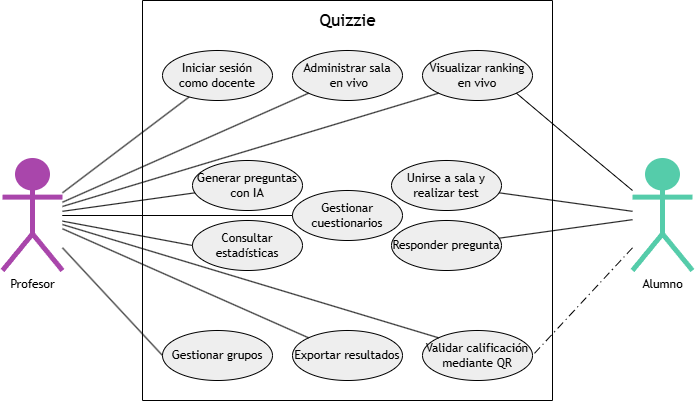
\includegraphics[width=0.95\textwidth]{figures/casos_de_uso.png}
    \vspace{0.5cm}
    \caption{Diagrama general de casos de uso del sistema.}
    \label{fig:diagrama_casos_uso}
\end{figure}

El conjunto de los casos de uso que componen el sistema es el siguiente:

\begin{itemize}
    \item \textbf{CU-01: Iniciar sesión como docente.} Permite al profesor acceder a su panel privado, registrarse o cerrar sesión de forma segura.
    \item \textbf{CU-02: Gestionar cuestionarios.} El profesor puede crear, editar, listar y eliminar sus bancos de preguntas.
    \item \textbf{CU-03: Generar preguntas con IA.} Extensión del CU-02 donde el profesor solicita a la IA la creación de borradores de preguntas basados en un tema.
    \item \textbf{CU-04: Administrar sala en vivo.} El profesor instancia un cuestionario, genera un PIN de acceso y controla el flujo de la partida (inicio, paso de preguntas y cierre).
    \item \textbf{CU-05: Unirse a sala y realizar test.} El alumno accede mediante PIN, responde a las preguntas sincronizadas y recibe feedback inmediato sobre su rendimiento.
    \item \textbf{CU-06: Visualizar ranking en vivo.} Los alumnos y el profesor visualizan la progresión de los líderes de la sala tras cada pregunta.
    \item \textbf{CU-07: Validar calificación mediante QR.} El profesor utiliza su dispositivo para escanear el código QR del alumno, verificando su identidad y presencia física para oficializar la calificación.
    \item \textbf{CU-08: Consultar estadísticas.} El profesor analiza los puntos críticos y el rendimiento general de la clase tras finalizar la sesión.
    \item \textbf{CU-09: Exportar resultados.} El profesor descarga los datos de los alumnos verificados en formato CSV para su uso en plataformas externas.
    \item \textbf{CU-10: Responder pregunta.} El alumno puede responder durante el tiempo determinado a las preguntas del test obteniendo la puntuación pertinente.
    \item \textbf{CU-11: Gestionar grupos.} El profesor organiza el alumnado creando etiquetas de grupo para asociar y evaluar la evolución histórica de un mismo conjunto de estudiantes.
\end{itemize}

\subsection{Especificación detallada de Casos de Uso}\label{sub:especificacion_casos_de_uso}

A continuación, se detallan las plantillas descriptivas de cada caso de uso del sistema, especificando sus actores, precondiciones, secuencias de pasos lógicos y la gestión de escenarios alternativos de error:

\begin{table}[H]
\centering
\small
\renewcommand{\arraystretch}{1.3}
\setlength{\tabcolsep}{6pt}
\makebox[\textwidth][c]{%
\begin{tabularx}{1.1\textwidth}{l Y}
\bighline
\multicolumn{2}{c}{\textbf{CU-01: Iniciar sesión como docente}\label{cu:01}} \\ \bighline
\textbf{Actor principal} & Profesor. \\ \hline
\textbf{Precondición} & El profesor debe estar registrado en la plataforma. \\ \hline
\textbf{Flujo principal} & 1. El profesor introduce su correo electrónico y contraseña en el formulario de login. \\ \cline{2-2}
                         & 2. El sistema cifra la contraseña introducida y la compara con el \textit{hash} almacenado. \\ \cline{2-2}
                         & 3. El sistema genera un token de sesión (JWT) y redirige al profesor a su panel principal. \\ \hline
\textbf{Flujo alternativo} & Si las credenciales son incorrectas, el sistema muestra un mensaje de error y permite reintentar el acceso. \\ \bighline
\end{tabularx}%
}
\caption[CU-01: Iniciar sesión como docente]{Especificación del caso de uso CU-01.}
\label{tab:cu_01}
\end{table}

\vfill

\begin{table}[H]
\centering
\small
\renewcommand{\arraystretch}{1.3}
\setlength{\tabcolsep}{6pt}
\makebox[\textwidth][c]{%
\begin{tabularx}{1.1\textwidth}{l Y}
\bighline
\multicolumn{2}{c}{\textbf{CU-02: Gestionar cuestionarios}\label{cu:02}} \\ \bighline
\textbf{Actor principal} & Profesor. \\ \hline
\textbf{Precondición} & El profesor ha iniciado sesión correctamente. \\ \hline
\textbf{Flujo principal} & 1. El profesor accede a su biblioteca de contenidos. \\ \cline{2-2}
                         & 2. Selecciona la opción de crear un nuevo cuestionario o editar uno existente. \\ \cline{2-2}
                         & 3. El profesor define el título, descripción y añade preguntas con sus respectivas opciones. \\ \cline{2-2}
                         & 4. El profesor marca la opción correcta para cada pregunta y asigna una puntuación. \\ \cline{2-2}
                         & 5. El sistema guarda los cambios en la base de datos permanente. \\ \hline
\textbf{Postcondición} & El cuestionario queda disponible para ser utilizado en una sala. \\ \bighline
\end{tabularx}%
}
\caption[CU-02: Gestionar cuestionarios]{Especificación del caso de uso CU-02.}
\label{tab:cu_02}
\end{table}

\newpage

\begin{table}[H]
\centering
\small
\renewcommand{\arraystretch}{1.2}
\setlength{\tabcolsep}{6pt}
\makebox[\textwidth][c]{%
\begin{tabularx}{1.1\textwidth}{l Y}
\bighline
\multicolumn{2}{c}{\textbf{CU-03: Generar preguntas con IA}\label{cu:03}} \\ \bighline
\textbf{Actores} & Principal: Profesor. Secundario: Servicio de IA (API). \\ \hline
\textbf{Precondición} & El profesor se encuentra dentro del editor de cuestionarios. \\ \hline
\textbf{Flujo principal} & 1. El profesor activa el asistente de IA e introduce un tema o pega un texto base. \\ \cline{2-2}
                         & 2. El sistema envía la información a la API de IA externa. \\ \cline{2-2}
                         & 3. El sistema recibe y presenta al profesor un listado de preguntas y respuestas sugeridas. \\ \cline{2-2}
                         & 4. El profesor selecciona las preguntas que desea importar y las edita si es necesario. \\ \cline{2-2}
                         & 5. El sistema integra las preguntas seleccionadas en el cuestionario actual. \\ \bighline
\end{tabularx}%
}
\caption[CU-03: Generar preguntas con IA]{Especificación del caso de uso CU-03.}\label{tab:cu_03}
\end{table}

\vfill

\begin{table}[H]
\centering
\small
\renewcommand{\arraystretch}{1.2}
\setlength{\tabcolsep}{6pt}
\makebox[\textwidth][c]{%
\begin{tabularx}{1.1\textwidth}{l Y}
\bighline
\multicolumn{2}{c}{\textbf{CU-04: Administrar sala en vivo}\label{cu:04}} \\ \bighline
\textbf{Actor principal} & Profesor. \\ \hline
\textbf{Precondición} & El profesor está autenticado y ha seleccionado un cuestionario de su biblioteca. \\ \hline
\textbf{Flujo principal} & 1. El profesor solicita la creación de una nueva sala de juego. \\ \cline{2-2}
                         & 2. El sistema genera un PIN único de 6 dígitos y abre el \textit{socket} de comunicación. \\ \cline{2-2}
                         & 3. El profesor controla en tiempo real la entrada de alumnos en la sala de espera. \\ \cline{2-2}
                         & 4. El profesor inicia el test, enviando la señal de comienzo a todos los alumnos. \\ \cline{2-2}
                         & 5. El profesor controla el paso de las preguntas o permite el avance automático. \\ \cline{2-2}
                         & 6. El profesor finaliza la sesión manualmente o al terminar las preguntas. \\ \bighline
\end{tabularx}%
}
\caption[CU-04: Administrar sala en vivo]{Especificación del caso de uso CU-04.}\label{tab:cu_04}
\end{table}

\vfill

\begin{table}[H]
\centering
\small
\renewcommand{\arraystretch}{1.2}
\setlength{\tabcolsep}{6pt}
\makebox[\textwidth][c]{%
\begin{tabularx}{1.1\textwidth}{l Y}
\bighline
\multicolumn{2}{c}{\textbf{CU-05: Unirse a sala y realizar test}\label{cu:05}} \\ \bighline
\textbf{Actor principal} & Alumno. \\ \hline
\textbf{Precondición} & Existe una sala activa y el alumno posee el código PIN. \\ \hline
\textbf{Flujo principal} & 1. El alumno introduce el PIN y un \textit{nickname}. \\ \cline{2-2}
                         & 2. El sistema valida el acceso y posiciona al alumno en la sala de espera. \\ \cline{2-2}
                         & 3. Al comenzar el test, el alumno recibe las preguntas de forma sincronizada con el resto de la clase. \\ \cline{2-2}
                         & 4. El alumno selecciona la opción deseada dentro del tiempo límite. \\ \cline{2-2}
                         & 5. El sistema registra la respuesta y el tiempo empleado. \\ \cline{2-2}
                         & 6. Al finalizar el \textit{quiz}, el alumno recibe un código QR único de validación. \\ \hline
\textbf{Flujo alternativo} & Si el alumno sufre una desconexión, puede reingresar con el mismo PIN y \textit{nickname}; el sistema restaurará su sesión y lo situará en la pregunta activa. \\ \bighline
\end{tabularx}%
}
\caption[CU-05: Unirse a sala y realizar test]{Especificación del caso de uso CU-05.}
\label{tab:cu_05}
\end{table}

\newpage

\begin{table}[H]
\centering
\small
\renewcommand{\arraystretch}{1.25}
\setlength{\tabcolsep}{6pt}
\makebox[\textwidth][c]{%
\begin{tabularx}{1.1\textwidth}{l Y}
\bighline
\multicolumn{2}{c}{\textbf{CU-06: Visualizar ranking en vivo}\label{cu:06}} \\ \bighline
\textbf{Actores} & Principal: Profesor / Alumno. \\ \hline
\textbf{Precondición} & Se ha completado al menos una pregunta en una sala activa. \\ \hline
\textbf{Flujo principal} & 1. El sistema calcula la puntuación de cada alumno basándose en aciertos y velocidad de respuesta. \\ \cline{2-2}
                         & 2. El sistema actualiza el ranking global de la sala. \\ \cline{2-2}
                         & 3. El profesor visualiza el ``Top 5'' en la pantalla principal para motivar a la clase. \\ \cline{2-2}
                         & 4. El alumno visualiza su posición relativa y sus puntos en su propio dispositivo. \\ \bighline
\end{tabularx}%
}
\caption[CU-06: Visualizar ranking en vivo]{Especificación del caso de uso CU-06.}
\label{tab:cu_06}
\end{table}

\vfill

\begin{table}[H]
\centering
\small
\renewcommand{\arraystretch}{1.25}
\setlength{\tabcolsep}{6pt}
\makebox[\textwidth][c]{%
\begin{tabularx}{1.1\textwidth}{l Y}
\bighline
\multicolumn{2}{c}{\textbf{CU-07: Validar calificación mediante QR}\label{cu:07}} \\ \bighline
\textbf{Actores} & Principal: Profesor. Secundario: Alumno. \\ \hline
\textbf{Precondición} & La sala ha finalizado y el alumno muestra el QR generado por el sistema. \\ \hline
\textbf{Flujo principal} & 1. El profesor selecciona la opción de ``Validar Alumno'' en su panel de sala. \\ \cline{2-2}
                         & 2. El profesor escanea el código QR del dispositivo del alumno. \\ \cline{2-2}
                         & 3. El sistema extrae el token cifrado del QR y lo valida contra el registro provisional en el backend. \\ \cline{2-2}
                         & 4. Tras la validación positiva, el sistema cambia el estado del alumno a ``Verificado''. \\ \cline{2-2}
                         & 5. La nota se hace persistente y se vincula oficialmente al registro del alumno. \\ \bighline
\end{tabularx}%
}
\caption[CU-07: Validar calificación mediante QR]{Especificación del caso de uso CU-07.}
\label{tab:cu_07}
\end{table}

\vfill

\begin{table}[H]
\centering
\small
\renewcommand{\arraystretch}{1.25}
\setlength{\tabcolsep}{6pt}
\makebox[\textwidth][c]{%
\begin{tabularx}{1.1\textwidth}{l Y}
\bighline
\multicolumn{2}{c}{\textbf{CU-08: Consultar estadísticas}\label{cu:08}} \\ \bighline
\textbf{Actor principal} & Profesor. \\ \hline
\textbf{Precondición} & Existen salas finalizadas con respuestas registradas. \\ \hline
\textbf{Flujo principal} & 1. El profesor accede al histórico de salas desde su panel. \\ \cline{2-2}
                         & 2. Selecciona una sesión específica para analizar. \\ \cline{2-2}
                         & 3. El sistema genera gráficas comparativas sobre el porcentaje de aciertos por pregunta. \\ \cline{2-2}
                         & 4. El profesor identifica las áreas de conocimiento donde los alumnos han tenido más dificultades. \\ \bighline
\end{tabularx}%
}
\caption[CU-08: Consultar estadísticas]{Especificación del caso de uso CU-08.}
\label{tab:cu_08}
\end{table}

\newpage

\begin{table}[H]
\centering
\small
\renewcommand{\arraystretch}{1.2}
\setlength{\tabcolsep}{6pt}
\makebox[\textwidth][c]{%
\begin{tabularx}{1.1\textwidth}{l Y}
\bighline
\multicolumn{2}{c}{\textbf{CU-09: Exportar resultados}\label{cu:09}} \\ \bighline
\textbf{Actor principal} & Profesor. \\ \hline
\textbf{Precondición} & La sala ha finalizado y existen alumnos con estado ``Verificado''. \\ \hline
\textbf{Flujo principal} & 1. El profesor solicita la exportación de resultados desde el informe de la sala. \\ \cline{2-2}
                         & 2. El sistema filtra los datos para incluir únicamente los resultados verificados. \\ \cline{2-2}
                         & 3. El sistema genera un archivo en formato CSV o Excel. \\ \cline{2-2}
                         & 4. El archivo se descarga automáticamente en el dispositivo del profesor. \\ \bighline
\end{tabularx}%
}
\caption[CU-09: Exportar resultados]{Especificación del caso de uso CU-09.}
\label{tab:cu_09}
\end{table}

\begin{table}[H]
\centering
\small
\renewcommand{\arraystretch}{1.2}
\setlength{\tabcolsep}{6pt}
\makebox[\textwidth][c]{%
\begin{tabularx}{1.1\textwidth}{l Y}
\bighline
\multicolumn{2}{c}{\textbf{CU-10: Responder pregunta}\label{cu:10}} \\ \bighline
\textbf{Actor principal} & Alumno. \\ \hline
\textbf{Precondición} & El alumno está en una sala activa y el profesor ha lanzado una pregunta. \\ \hline
\textbf{Flujo principal} & 1. El sistema muestra el enunciado y las opciones de respuesta en el dispositivo del alumno. \\ \cline{2-2}
                         & 2. El sistema inicia el cronómetro de cuenta atrás definido para esa sala. \\ \cline{2-2}
                         & 3. El alumno selecciona una de las opciones antes de que el tiempo se agote. \\ \cline{2-2}
                         & 4. El sistema captura la opción elegida y el tiempo de la respuesta (\textit{timestamp}). \\ \cline{2-2}
                         & 5. Al agotarse el tiempo o responder todos los alumnos, el sistema cierra la recepción de datos. \\ \cline{2-2}
                         & 6. El sistema mira si la respuesta es correcta y calcula los puntos obtenidos. \\ \hline
\textbf{Flujo alternativo} & Si el alumno no selecciona ninguna opción antes de que el cronómetro llegue a cero, el sistema registra la pregunta como ``No contestada'' con 0 puntos. \\ \hline
\textbf{Postcondición} & El resultado de la pregunta se almacena temporalmente para actualizar el ranking en vivo. \\ \bighline
\end{tabularx}%
}
\caption[CU-10: Responder pregunta]{Especificación del caso de uso CU-10.}
\label{tab:cu_10}
\end{table}

\begin{table}[H]
\centering
\small
\renewcommand{\arraystretch}{1.2}
\setlength{\tabcolsep}{6pt}
\makebox[\textwidth][c]{%
\begin{tabularx}{1.1\textwidth}{l Y}
\bighline
\multicolumn{2}{c}{\textbf{CU-11: Gestionar grupos}\label{cu:11}} \\ \bighline
\textbf{Actor principal} & Profesor. \\ \hline
\textbf{Precondición} & El profesor ha iniciado sesión correctamente en el sistema. \\ \hline
\textbf{Flujo principal} & 1. El profesor accede a la sección de gestión de grupos desde el panel de control. \\ \cline{2-2}
                         & 2. Selecciona la opción de crear una nueva clase e introduce un nombre descriptivo o etiqueta de grupo. \\ \cline{2-2}
                         & 3. El profesor asocia la lista de identificadores de alumnos válidos correspondientes a ese conjunto académico. \\ \cline{2-2}
                         & 4. El sistema almacena la estructura del grupo vinculándola directamente al perfil del docente responsable. \\ \cline{2-2}
                         & 5. El profesor consulta los reportes específicos para comprobar el progreso y la evolución histórica de las calificaciones de dicha clase. \\ \bighline
\end{tabularx}%
}
\caption[CU-11: Gestionar grupos]{Especificación del caso de uso CU-11.}
\label{tab:cu_11}
\end{table}

\section{Requisitos no funcionales}\label{sec:requisitos_no_funcionales}
Los requisitos no funcionales determinan los atributos de calidad, restricciones técnicas y criterios de rendimiento que debe satisfacer la plataforma \textit{Quizzie}. Su categorización se articula atendiendo a las dimensiones del modelo de calidad del producto de software definido en la norma ISO/IEC 25010 \cite{iso25010}:

\begin{table}[H]
\centering
\small
\renewcommand{\arraystretch}{1.35}
\makebox[\textwidth][c]{%
\begin{tabularx}{1.06\textwidth}{l l P{2.6cm} Y}
\bighline
\textbf{Dimensión} & \textbf{ID} & \textbf{Nombre} & \textbf{Descripción} \\ \bighline
Rendimiento & RNF-01\label{rnf:01} & Sincronización & Los eventos en tiempo real deben procesarse de forma óptima en el backend para garantizar la coherencia síncrona en el aula. \\ \cline{2-4}
            & RNF-02\label{rnf:02} & Concurrencia & Soporte mínimo de 100 alumnos interactuando de forma simultánea dentro de una misma sala sin degradación de los servicios básicos. \\ \hline
Seguridad   & RNF-03\label{rnf:03} & Integridad & El token de validación presencial embebido en el QR del alumno debe ser criptográficamente seguro, firmado por el servidor y no falsificable. \\ \cline{2-4}
            & RNF-04\label{rnf:04} & Privacidad & Almacenamiento e inserción obligatoria de credenciales de acceso de profesores mediante algoritmos de \textit{hashing} seguro y unidireccional. \\ \cline{2-4}
            & RNF-05\label{rnf:05} & Cifrado & Uso estricto de canales de red protegidos bajo protocolos de comunicación seguros HTTPS y \textit{WebSockets} seguros (\texttt{WSS}). \\ \hline
Usabilidad  & RNF-06\label{rnf:06} & Adaptabilidad & Interfaz de usuario adaptativa (\textit{Responsive Design}) optimizada para una navegación fluida tanto en dispositivos móviles como en ordenadores. \\ \cline{2-4}
            & RNF-07\label{rnf:07} & Eficiencia QR & Optimización del flujo óptico para que el tiempo de lectura, decodificación y validación de la firma del código QR por la cámara sea inmediato. \\ \hline
Fiabilidad  & RNF-08\label{rnf:08} & Reconexión & Capacidad de retener y recuperar el estado lógico y la puntuación transitoria de un participante ante caídas o pérdidas accidentales de conectividad. \\ \hline
Disponibilidad & RNF-09\label{rnf:09} & Persistencia & Mecanismo de salvaguarda y respaldo de los resultados provisionales en el backend ante interrupciones críticas o fallos imprevistos del servidor. \\ \hline
Mantenibilidad & RNF-10\label{rnf:10} & Modularidad & Separación clara de responsabilidades entre el servidor de base de datos, el backend y el cliente frontend para facilitar futuras actualizaciones. \\ \bighline
\end{tabularx}%
}
\caption{Requisitos no funcionales clasificados por dimensión.}
\label{tab:requisitos_no_funcionales}
\end{table}

\section{Trazabilidad de requisitos}\label{sec:trazabilidad_de_requisitos}
Para garantizar la integridad del desarrollo y demostrar el cumplimiento de las metas del proyecto, este apartado presenta la trazabilidad bidireccional del sistema. Este proceso permite certificar que cada decisión responde directamente a un fin práctico de la aplicación, evitando la existencia de elementos redundantes o injustificados. Las tres matrices que se muestran a continuación relacionan objetivos funcionales con requisitos de información, requisitos no funcionales y requisitos funcionales, respectivamente.

\begin{table}[H]
\centering
\small
\renewcommand{\arraystretch}{1.3}
\setlength{\tabcolsep}{2.5pt}
\makebox[\textwidth][c]{%
\begin{tabularx}{\textwidth}{>{\centering\arraybackslash}m{1.35cm} *{12}{>{\centering\arraybackslash}X}}
\bighline
\diagbox[width=1.35cm, height=0.85cm]{\raisebox{1.5pt}{\scriptsize\textbf{RI}}}{\raisebox{-1.5pt}{\scriptsize\textbf{OBJ}}} & 
\hyperref[obj:01]{01} & 
\hyperref[obj:02]{02} & 
\hyperref[obj:03]{03} & 
\hyperref[obj:04]{04} & 
\hyperref[obj:05]{05} & 
\hyperref[obj:06]{06} & 
\hyperref[obj:07]{07} & 
\hyperref[obj:08]{08} & 
\hyperref[obj:09]{09} & 
\hyperref[obj:10]{10} & 
\hyperref[obj:11]{11} & 
\hyperref[obj:12]{12} \\ \bighline
\hyperref[ri:01]{01} & \traceCrossGray & & & & & & & & & & & \\ \hline
\hyperref[ri:02]{02} & & \traceCross & & & & & & & \traceCrossGray & & & \\ \hline
\hyperref[ri:03]{03} & & & \traceCrossGray & \traceCross & \traceCrossGray & & & & & & & \\ \hline
\hyperref[ri:04]{04} & & & & & \traceCrossGray & \traceCross & \traceCrossGray & \traceCross & & & & \\ \hline
\hyperref[ri:05]{05} & & & & & & & \traceCrossGray & \traceCross & & & & \traceCross \\ \hline
\hyperref[ri:06]{06} & & & & & & & & & & & \traceCrossGray & \traceCross \\ \bighline
\end{tabularx}%
}
\caption{Matriz de trazabilidad RI-OBJ.}
\label{tab:matriz_trazabilidad_ri_obj}
\end{table}

\begin{table}[H]
\centering
\small
\renewcommand{\arraystretch}{1.3}
\setlength{\tabcolsep}{2.5pt}
\makebox[\textwidth][c]{%
\begin{tabularx}{\textwidth}{>{\centering\arraybackslash}m{1.35cm} *{12}{>{\centering\arraybackslash}X}}
\bighline
\diagbox[width=1.35cm, height=0.85cm]{\raisebox{1.5pt}{\scriptsize\textbf{RNF}}}{\raisebox{-1.5pt}{\scriptsize\textbf{OBJ}}} & 
\hyperref[obj:01]{01} & 
\hyperref[obj:02]{02} & 
\hyperref[obj:03]{03} & 
\hyperref[obj:04]{04} & 
\hyperref[obj:05]{05} & 
\hyperref[obj:06]{06} & 
\hyperref[obj:07]{07} & 
\hyperref[obj:08]{08} & 
\hyperref[obj:09]{09} & 
\hyperref[obj:10]{10} & 
\hyperref[obj:11]{11} & 
\hyperref[obj:12]{12} \\ \bighline
\hyperref[rnf:01]{01} & & & & & \traceCrossGray & & & & & & & \\ \hline
\hyperref[rnf:02]{02} & & & & & \traceCrossGray & & & & & & & \\ \hline
\hyperref[rnf:03]{03} & & & & & & \traceCross & \traceCrossGray & & & & & \\ \hline
\hyperref[rnf:04]{04} & \traceCrossGray & & & & & & & & & & & \\ \hline
\hyperref[rnf:05]{05} & \traceCrossGray & & & & \traceCrossGray & & & & & & & \\ \hline
\hyperref[rnf:06]{06} & \traceCrossGray & \traceCross & & \traceCross & \traceCrossGray & & & & & & & \\ \hline
\hyperref[rnf:07]{07} & & & & & & & & & & \traceCross & & \\ \hline
\hyperref[rnf:08]{08} & & & & & \traceCrossGray & & & & & & & \\ \hline
\hyperref[rnf:09]{09} & & & \traceCrossGray & & \traceCrossGray & & \traceCrossGray & & & & & \\ \hline
\hyperref[rnf:10]{10} & \traceCrossGray & \traceCross & \traceCrossGray & \traceCross & \traceCrossGray & \traceCross & \traceCrossGray & \traceCross & \traceCrossGray & \traceCross & \traceCrossGray & \traceCross \\ \bighline
\end{tabularx}%
}
\caption{Matriz de trazabilidad RNF-OBJ.}
\label{tab:matriz_trazabilidad_rnf_obj}
\end{table}

\begin{table}[H]
\centering
\small
\renewcommand{\arraystretch}{0.95}
\setlength{\tabcolsep}{2.5pt}
\makebox[\textwidth][c]{%
\begin{tabularx}{\textwidth}{>{\centering\arraybackslash}m{1.35cm} *{12}{>{\centering\arraybackslash}X}}
\bighline
\diagbox[width=1.35cm, height=0.7cm]{\raisebox{1pt}{\scriptsize\textbf{RF}}}{\raisebox{-1pt}{\scriptsize\textbf{OBJ}}} & 
\hyperref[obj:01]{01} & 
\hyperref[obj:02]{02} & 
\hyperref[obj:03]{03} & 
\hyperref[obj:04]{04} & 
\hyperref[obj:05]{05} & 
\hyperref[obj:06]{06} & 
\hyperref[obj:07]{07} & 
\hyperref[obj:08]{08} & 
\hyperref[obj:09]{09} & 
\hyperref[obj:10]{10} & 
\hyperref[obj:11]{11} & 
\hyperref[obj:12]{12} \\ \bighline
\hyperref[req:01]{01} & \traceCrossGray & & & & & & & & & & & \\ \hline
\hyperref[req:02]{02} & \traceCrossGray & & & & & & & & & & & \\ \hline
\hyperref[req:03]{03} & \traceCrossGray & & & & & & & & & & & \\ \hline
\hyperref[req:04]{04} & \traceCrossGray & & & & & & & & & & & \\ \hline
\hyperref[req:05]{05} & \traceCrossGray & & & & & & & & & & & \\ \hline
\hyperref[req:06]{06} & \traceCrossGray & & & & & & & & & & & \\ \hline
\hyperref[req:07]{07} & & \traceCross & & & & & & & & & & \\ \hline
\hyperref[req:08]{08} & & \traceCross & & & & & & & & & & \\ \hline
\hyperref[req:09]{09} & & & & & & & & \traceCross & & & & \\ \hline
\hyperref[req:10]{10} & & \traceCross & & & & & & & & & & \\ \hline
\hyperref[req:11]{11} & & & \traceCrossGray & & & & & & & & & \\ \hline
\hyperref[req:12]{12} & & & & & & & & & & & & \traceCross \\ \hline
\hyperref[req:13]{13} & & \traceCross & & & & & & & & & & \\ \hline
\hyperref[req:14]{14} & & \traceCross & & & & & & & & & & \\ \hline
\hyperref[req:15]{15} & & & \traceCrossGray & & & & & & & & & \\ \hline
\hyperref[req:16]{16} & & & & \traceCross & & & & & & & & \\ \hline
\hyperref[req:17]{17} & & & & \traceCross & & & & & & & & \\ \hline
\hyperref[req:18]{18} & & & \traceCrossGray & & & & & & & & & \\ \hline
\hyperref[req:19]{19} & & & \traceCrossGray & & & & & & & & & \\ \hline
\hyperref[req:20]{20} & & & & & \traceCrossGray & & & & & & & \\ \hline
\hyperref[req:21]{21} & & & & & \traceCrossGray & & & & & & & \\ \hline
\hyperref[req:22]{22} & & & \traceCrossGray & & & & & & & & & \\ \hline
\hyperref[req:23]{23} & & & & & \traceCrossGray & & & & & & & \\ \hline
\hyperref[req:24]{24} & & & & & \traceCrossGray & & & & & & & \\ \hline
\hyperref[req:25]{25} & & & & & & & \traceCrossGray & & & & & \\ \hline
\hyperref[req:26]{26} & & & & & & \traceCross & & & & & & \\ \hline
\hyperref[req:27]{27} & & & & & & & & & & \traceCross & & \\ \hline
\hyperref[req:28]{28} & & & & & & & & & & \traceCross & & \\ \hline
\hyperref[req:29]{29} & & & & & & \traceCross & & & & & & \\ \hline
\hyperref[req:30]{30} & & & & & & & \traceCrossGray & & & & & \\ \hline
\hyperref[req:31]{31} & & & & & & & \traceCrossGray & & & & & \\ \hline
\hyperref[req:32]{32} & & & & & & & & \traceCross & & & & \\ \hline
\hyperref[req:33]{33} & & & & & & & & \traceCross & & & & \\ \hline
\hyperref[req:34]{34} & & & & & & & & & \traceCrossGray & & & \\ \hline
\hyperref[req:35]{35} & & & & & & & & & \traceCrossGray & & & \\ \hline
\hyperref[req:36]{36} & & & & & & & & & \traceCrossGray & & & \\ \hline
\hyperref[req:37]{37} & & & & & & & & & \traceCrossGray & & & \\ \hline
\hyperref[req:38]{38} & & & & & & & & & & & \traceCrossGray & \\ \hline
\hyperref[req:39]{39} & & & & & & & & & & & & \traceCross \\ \hline
\hyperref[req:40]{40} & & & & & \traceCrossGray & & & & & & & \\ \hline
\hyperref[req:41]{41} & & \traceCross & & & & & & & & & & \\ \hline
\hyperref[req:42]{42} & & & & & \traceCrossGray & & & & & & & \\ \hline
\hyperref[req:43]{43} & & & & & \traceCrossGray & & & & & & & \\ \hline
\hyperref[req:44]{44} & & & \traceCrossGray & & & & & & & & & \\ \hline
\hyperref[req:45]{45} & & & \traceCrossGray & & & & & & & & & \\ \hline
\hyperref[req:46]{46} & & \traceCross & & & & & & & & & & \\ \hline
\hyperref[req:47]{47} & & & & & & & \traceCrossGray & & & & & \\ \bighline
\end{tabularx}%
}
\caption{Matriz de trazabilidad RF-OBJ.}
\label{tab:matriz_trazabilidad_rf_obj}
\end{table}

Por último, con el fin de unificar todo el ciclo de vida del desarrollo, se presenta la siguiente matriz de trazabilidad unificada. Este mapa conecta de manera jerárquica los módulos del sistema, los objetivos funcionales que persiguen, los casos de uso técnicos, y cómo estos se desglosan en las historias de usuario, compuestas por sus respectivos requisitos funcionales.

\begin{table}[H]
\centering
\small
\renewcommand{\arraystretch}{1.3}
\makebox[\textwidth][c]{
\begin{tabular}{llllp{7cm}}
\bighline
\textbf{Módulo} & \textbf{OBJ} & \textbf{CU} & \textbf{HU} & \textbf{RF} \\ \bighline
Contenido & \hyperref[obj:02]{OBJ-02} & \hyperref[cu:02]{CU-02} & \hyperref[hu:pr-01]{HU-PR-01} & \hyperref[req:07]{RF-07}, \hyperref[req:08]{RF-08}, \hyperref[req:10]{RF-10}, \hyperref[req:12]{RF-12} \\ \cline{4-5} 
          &                           &                           & \hyperref[hu:pr-02]{HU-PR-02} & \hyperref[req:13]{RF-13}, \hyperref[req:14]{RF-14}, \hyperref[req:41]{RF-41} \\ \cline{4-5} 
          &                           &                           & \hyperref[hu:pr-13]{HU-PR-13} & \hyperref[req:46]{RF-46} \\ \cline{2-5} 
          & \hyperref[obj:09]{OBJ-09} & \hyperref[cu:03]{CU-03} & \hyperref[hu:pr-09]{HU-PR-09} & \hyperref[req:34]{RF-34}, \hyperref[req:35]{RF-35}, \hyperref[req:36]{RF-36}, \hyperref[req:37]{RF-37} \\ \hline
Salas     & \hyperref[obj:03]{OBJ-03} & \hyperref[cu:04]{CU-04} & \hyperref[hu:pr-03]{HU-PR-03} & \hyperref[req:11]{RF-11}, \hyperref[req:15]{RF-15}, \hyperref[req:18]{RF-18}, \hyperref[req:22]{RF-22} \\ \cline{4-5} 
          &                           &                           & \hyperref[hu:pr-05]{HU-PR-05} & \hyperref[req:19]{RF-19} \\ \cline{4-5} 
          &                           &                           & \hyperref[hu:pr-11]{HU-PR-11} & \hyperref[req:42]{RF-42}, \hyperref[req:43]{RF-43}, \hyperref[req:44]{RF-44} \\ \cline{4-5} 
          &                           &                           & \hyperref[hu:pr-12]{HU-PR-12} & \hyperref[req:45]{RF-45} \\ \cline{2-5} 
          & \hyperref[obj:04]{OBJ-04} & \hyperref[cu:05]{CU-05} & \hyperref[hu:al-01]{HU-AL-01} & \hyperref[req:16]{RF-16}, \hyperref[req:17]{RF-17}, \hyperref[req:40]{RF-40} \\ \cline{2-5} 
          & \hyperref[obj:05]{OBJ-05} & \hyperref[cu:05]{CU-05} & \hyperref[hu:al-01]{HU-AL-01} & \hyperref[req:16]{RF-16}, \hyperref[req:17]{RF-17}, \hyperref[req:40]{RF-40} \\ \cline{3-5} 
          &                           & \hyperref[cu:10]{CU-10} & \hyperref[hu:al-02]{HU-AL-02} & \hyperref[req:20]{RF-20}, \hyperref[req:21]{RF-21} \\ \cline{4-5} 
          &                           &                           & \hyperref[hu:al-03]{HU-AL-03} & \hyperref[req:23]{RF-23}, \hyperref[req:24]{RF-24}, \hyperref[req:42]{RF-42}, \hyperref[req:43]{RF-43} \\ \cline{2-5} 
          & \hyperref[obj:06]{OBJ-06} & \hyperref[cu:07]{CU-07} & \hyperref[hu:pr-06]{HU-PR-06} & \hyperref[req:27]{RF-27}, \hyperref[req:28]{RF-28}, \hyperref[req:29]{RF-29}, \hyperref[req:30]{RF-30}, \hyperref[req:31]{RF-31} \\ \cline{4-5} 
          &                           &                           & \hyperref[hu:al-04]{HU-AL-04} & \hyperref[req:25]{RF-25}, \hyperref[req:26]{RF-26} \\ \cline{2-5} 
          & \hyperref[obj:07]{OBJ-07} & \hyperref[cu:07]{CU-07} & \hyperref[hu:pr-06]{HU-PR-06} & \hyperref[req:27]{RF-27}, \hyperref[req:28]{RF-28}, \hyperref[req:29]{RF-29}, \hyperref[req:30]{RF-30}, \hyperref[req:31]{RF-31} \\ \cline{4-5} 
          &                           &                           & \hyperref[hu:al-04]{HU-AL-04} & \hyperref[req:25]{RF-25}, \hyperref[req:26]{RF-26} \\ \cline{2-5} 
          & \hyperref[obj:08]{OBJ-08} & \hyperref[cu:06]{CU-06} & \hyperref[hu:pr-04]{HU-PR-04} & \hyperref[req:32]{RF-32} \\ \cline{4-5} 
          &                           &                           & \hyperref[hu:pr-12]{HU-PR-12} & \hyperref[req:09]{RF-09} \\ \cline{3-5} 
          &                           & \hyperref[cu:08]{CU-08} & \hyperref[hu:pr-08]{HU-PR-08} & \hyperref[req:33]{RF-33} \\ \cline{4-5} 
          &                           &                           & \hyperref[hu:pr-14]{HU-PR-14} & \hyperref[req:47]{RF-47} \\ \cline{2-5} 
          & \hyperref[obj:10]{OBJ-10} & \hyperref[cu:07]{CU-07} & \hyperref[hu:pr-06]{HU-PR-06} & \hyperref[req:27]{RF-27}, \hyperref[req:28]{RF-28}, \hyperref[req:29]{RF-29}, \hyperref[req:30]{RF-30}, \hyperref[req:31]{RF-31} \\ \cline{4-5} 
          &                           &                           & \hyperref[hu:al-04]{HU-AL-04} & \hyperref[req:25]{RF-25}, \hyperref[req:26]{RF-26} \\ \cline{2-5} 
          & \hyperref[obj:12]{OBJ-12} & \hyperref[cu:09]{CU-09} & \hyperref[hu:pr-10]{HU-PR-10} & \hyperref[req:39]{RF-39} \\ \hline
Usuarios  & \hyperref[obj:01]{OBJ-01} & \hyperref[cu:01]{CU-01} & \hyperref[hu:pr-01]{HU-PR-01} & \hyperref[req:01]{RF-01}, \hyperref[req:02]{RF-02}, \hyperref[req:03]{RF-03}, \hyperref[req:04]{RF-04}, \hyperref[req:05]{RF-05}, \hyperref[req:06]{RF-06} \\ \cline{2-5} 
          & \hyperref[obj:11]{OBJ-11} & \hyperref[cu:11]{CU-11} & \hyperref[hu:pr-07]{HU-PR-07} & \hyperref[req:38]{RF-38} \\ \bighline
\end{tabular}
}
\caption{Matriz de trazabilidad unificada del sistema.}
\label{tab:matriz_trazabilidad}
\end{table}
    \chapter{Diseño y arquitectura}\label{cap:diseno_y_arquitectura}

En este capítulo se describe la estructura técnica y conceptual sobre la que se asienta el sistema, detallando las decisiones arquitectónicas que garantizan su correcto funcionamiento, mantenibilidad y rendimiento. El diseño propuesto responde tanto a los requisitos funcionales del proyecto como a sus restricciones operativas: la ejecución de cuestionarios en tiempo real, la baja latencia en la transmisión de eventos a múltiples participantes simultáneos y una rigurosa separación de responsabilidades entre el cliente y el servidor.

\section{Patrones arquitectónicos elegidos}

Antes de seleccionar el \textit{stack} y la estructura del código, se establecieron una serie de principios de diseño orientados a garantizar la integridad de las calificaciones, la seguridad del sistema y su capacidad de escalado:

\begin{itemize}
    \item \textbf{Validación centralizada y control de roles (\textit{anti-cheat}):} El cliente no toma decisiones sobre la corrección de respuestas, cálculo de puntuaciones ni temporización oficial. Existe una estricta división de responsabilidades en la que las acciones administrativas (como el control del avance de preguntas o el cierre de salas) quedan reservadas exclusivamente al profesor. El alumno se limita únicamente a unirse a la sala y enviar sus respuestas.   
    \item \textbf{Desacoplamiento de la presentación y los datos:} El servidor se limita a enviar los datos y eventos de la partida, dejando que la aplicación del usuario se ocupe exclusivamente de cómo mostrar la información en pantalla, gestionar las animaciones y adaptarse a cada dispositivo.
    \item \textbf{Autenticación sin estado (\textit{stateless}):} La validación de identidades mediante tokens integrados en las cabeceras de cada solicitud evita el almacenamiento de estado de sesión en la memoria del servidor, facilitando la distribución de la carga.
    \item \textbf{Gestión de la concurrencia y escalabilidad:} El sistema debe ser capaz de mantener decenas de conexiones bidireccionales simultáneas en un aula sin bloquear el procesamiento del servidor, distribuyendo el rendimiento de forma eficiente entre peticiones HTTP habituales y eventos en tiempo real.
\end{itemize}

Para dar respuesta a estos principios, se ha optado por una arquitectura híbrida que combina tres patrones complementarios: \textbf{cliente-servidor desacoplado}, \textbf{arquitectura en capas} (\textit{layered architecture}) y \textbf{arquitectura basada en eventos} (\textit{event-driven architecture}).

\subsection{Arquitectura cliente-servidor desacoplada}

La aplicación adopta un esquema cliente-servidor desacoplado con una rigurosa delimitación de responsabilidades entre el cliente y el servidor:

\begin{itemize}
    \item \textbf{Cliente (\textit{frontend} - SPA):} Desarrollado como una (\textit{SPA (single page application)}), se encarga de la representación visual, la experiencia de usuario y el control de temporizadores locales de apoyo. Opera sin acceso directo a la persistencia ni a las reglas de negocio.
    \item \textbf{Servidor (\textit{backend} - API REST + WebSockets):} Actúa como la única fuente de verdad (\textit{single source of truth}), gestionando la autenticación, la seguridad criptográfica, el ciclo de vida de los cuestionarios, la persistencia en base de datos y la orquestación síncrona de las salas.
    \item \textbf{Canales de comunicación:}
    \begin{itemize}
        \item \textit{HTTP/HTTPS (API REST):} Empleado para operaciones síncronas sin estado, tales como el inicio de sesión, la gestión de cuestionarios y la consulta de informes históricos.
        \item \textit{WebSockets:} Empleado para mantener un canal de comunicación persistente, bidireccional y de baja latencia durante la ejecución en vivo de los cuestionarios.
    \end{itemize}
\end{itemize}

\subsection{Arquitectura en capas}
Tanto en el servidor como en el cliente, el sistema se estructura internamente en niveles independientes para aislar responsabilidades (\textit{separation of concerns}).

En el \textit{backend}, la lógica se organiza en cuatro capas conceptuales:
\begin{enumerate}
    \item \textbf{Capa de presentación y controladores:} Expone los puntos de entrada HTTP (endpoints REST) y los canales WebSocket. Valida las peticiones de entrada, gestiona las respuestas de la API y coordina la autenticación.
    \item \textbf{Capa de lógica de negocio y servicios:} Implementa las reglas del dominio:  suma de puntuaciones por respuesta, transiciones de estado de las salas, opciones de cuestionario en vivo y lógica de verificación.
    \item \textbf{Capa de acceso a datos y modelado (ORM):} Mapea las entidades de negocio del dominio con el modelo relacional, garantizando las restricciones de integridad y las relaciones entre entidades.
    \item \textbf{Capa de persistencia:} Administra la conexión con el motor de base de datos relacional y gestiona las transacciones de lectura y escritura.
\end{enumerate}

En el \textit{frontend}, la arquitectura reproduce este aislamiento separando la \textbf{capa de vistas} (componentes de interfaz), la \textbf{capa de estado y contexto} (sesión de usuario y datos de partida), la \textbf{capa de servicios de red} (módulos REST y sockets) y la \textbf{capa de contratos de datos} (definición de tipos e interfaces).

\subsection{Arquitectura basada en eventos}
Para las sesiones en tiempo real, el sistema adopta una arquitectura basada en eventos que mantiene sincronizados a todos los participantes conectados a una sala.

\begin{figure}[H]
    \centering
    \makebox[0pt][c]{
        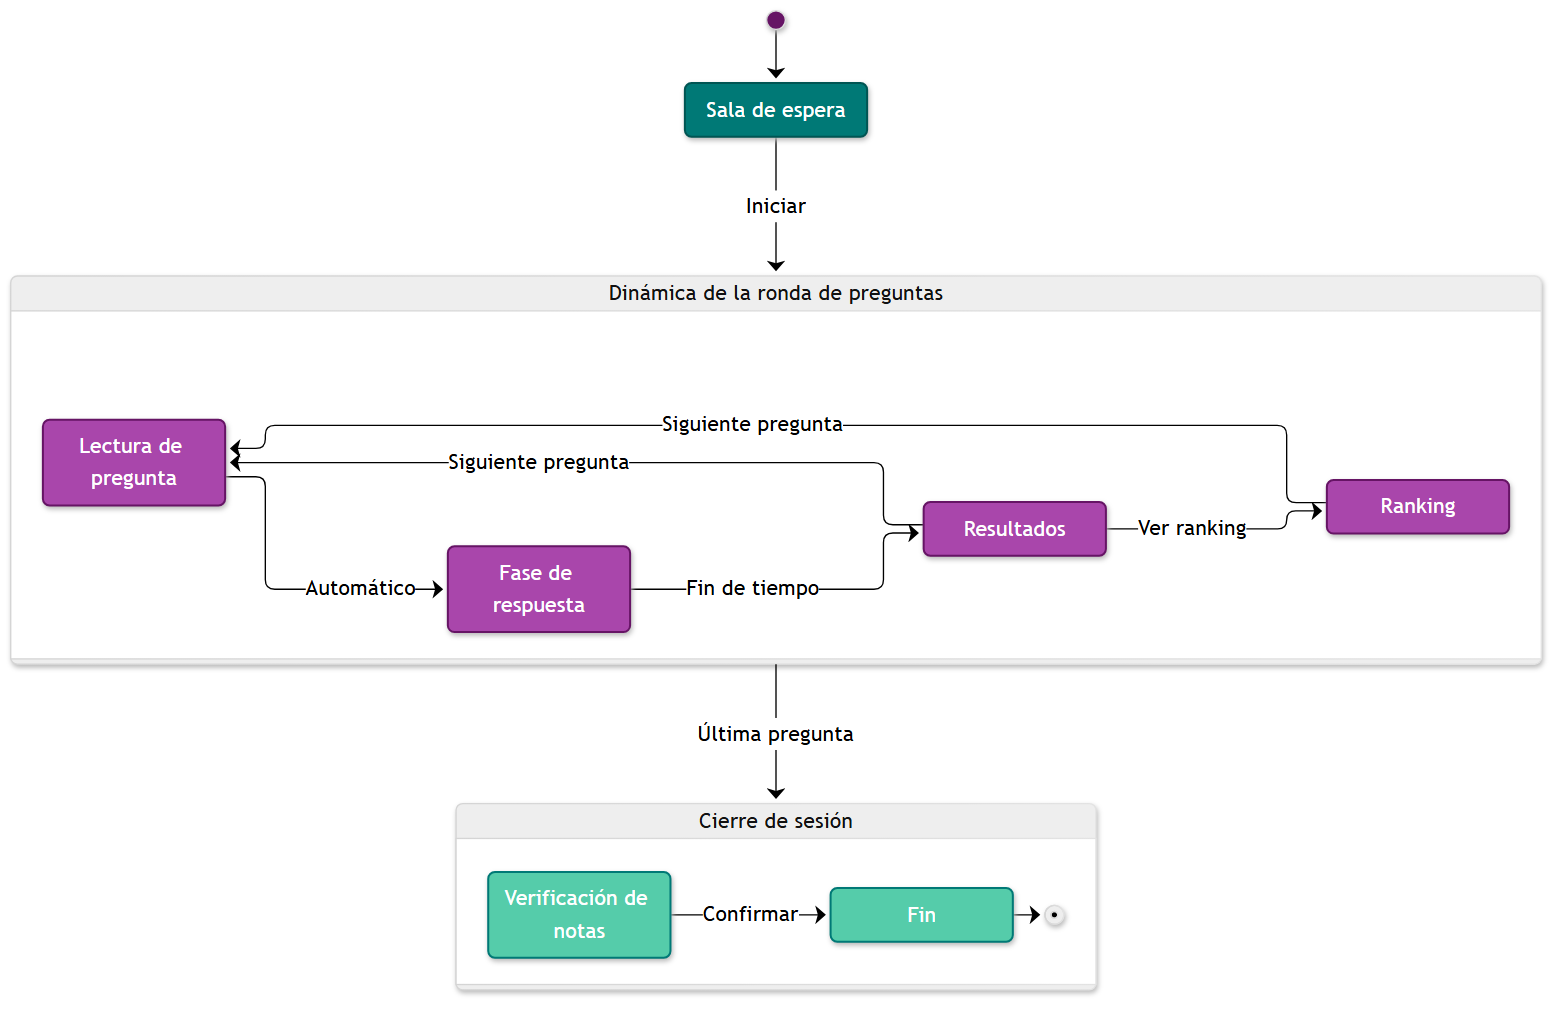
\includegraphics[width=1.2\textwidth]{figures/estados_sala.png}
    }
    \caption{Estados de la sala de juego en tiempo real.}
    \label{fig:estados_sala}
\end{figure}

El diseño de este comportamiento se apoya en los siguientes componentes conceptuales:
\begin{itemize}
    \item \textbf{Gestor centralizado de conexiones:} Mantiene el registro de las sesiones activas en memoria, administrando el ciclo de vida de los sockets y aplicando el patrón de difusión (\textit{broadcasting}) para emitir instrucciones a todos los participantes de una sala de forma simultánea.
    \item \textbf{Bucle de sincronización temporal:} Proceso asíncrono en segundo plano que supervisa el transcurso del tiempo de respuesta en las salas activas, notifica el tiempo restante periódicamente y desencadena automáticamente la transición de fase al expirar el tiempo.
    \item \textbf{Ciclo de eventos y transmisión:} Los cambios de estado de la sala (fase de lectura, apertura de respuestas, muestra de resultados, actualización de temporizadores) se propagan como eventos estructurados JSON, permitiendo que la interfaz del cliente reaccione de forma inmediata.
\end{itemize}

\begin{figure}[H]
    \centering
    \makebox[0pt][c]{
        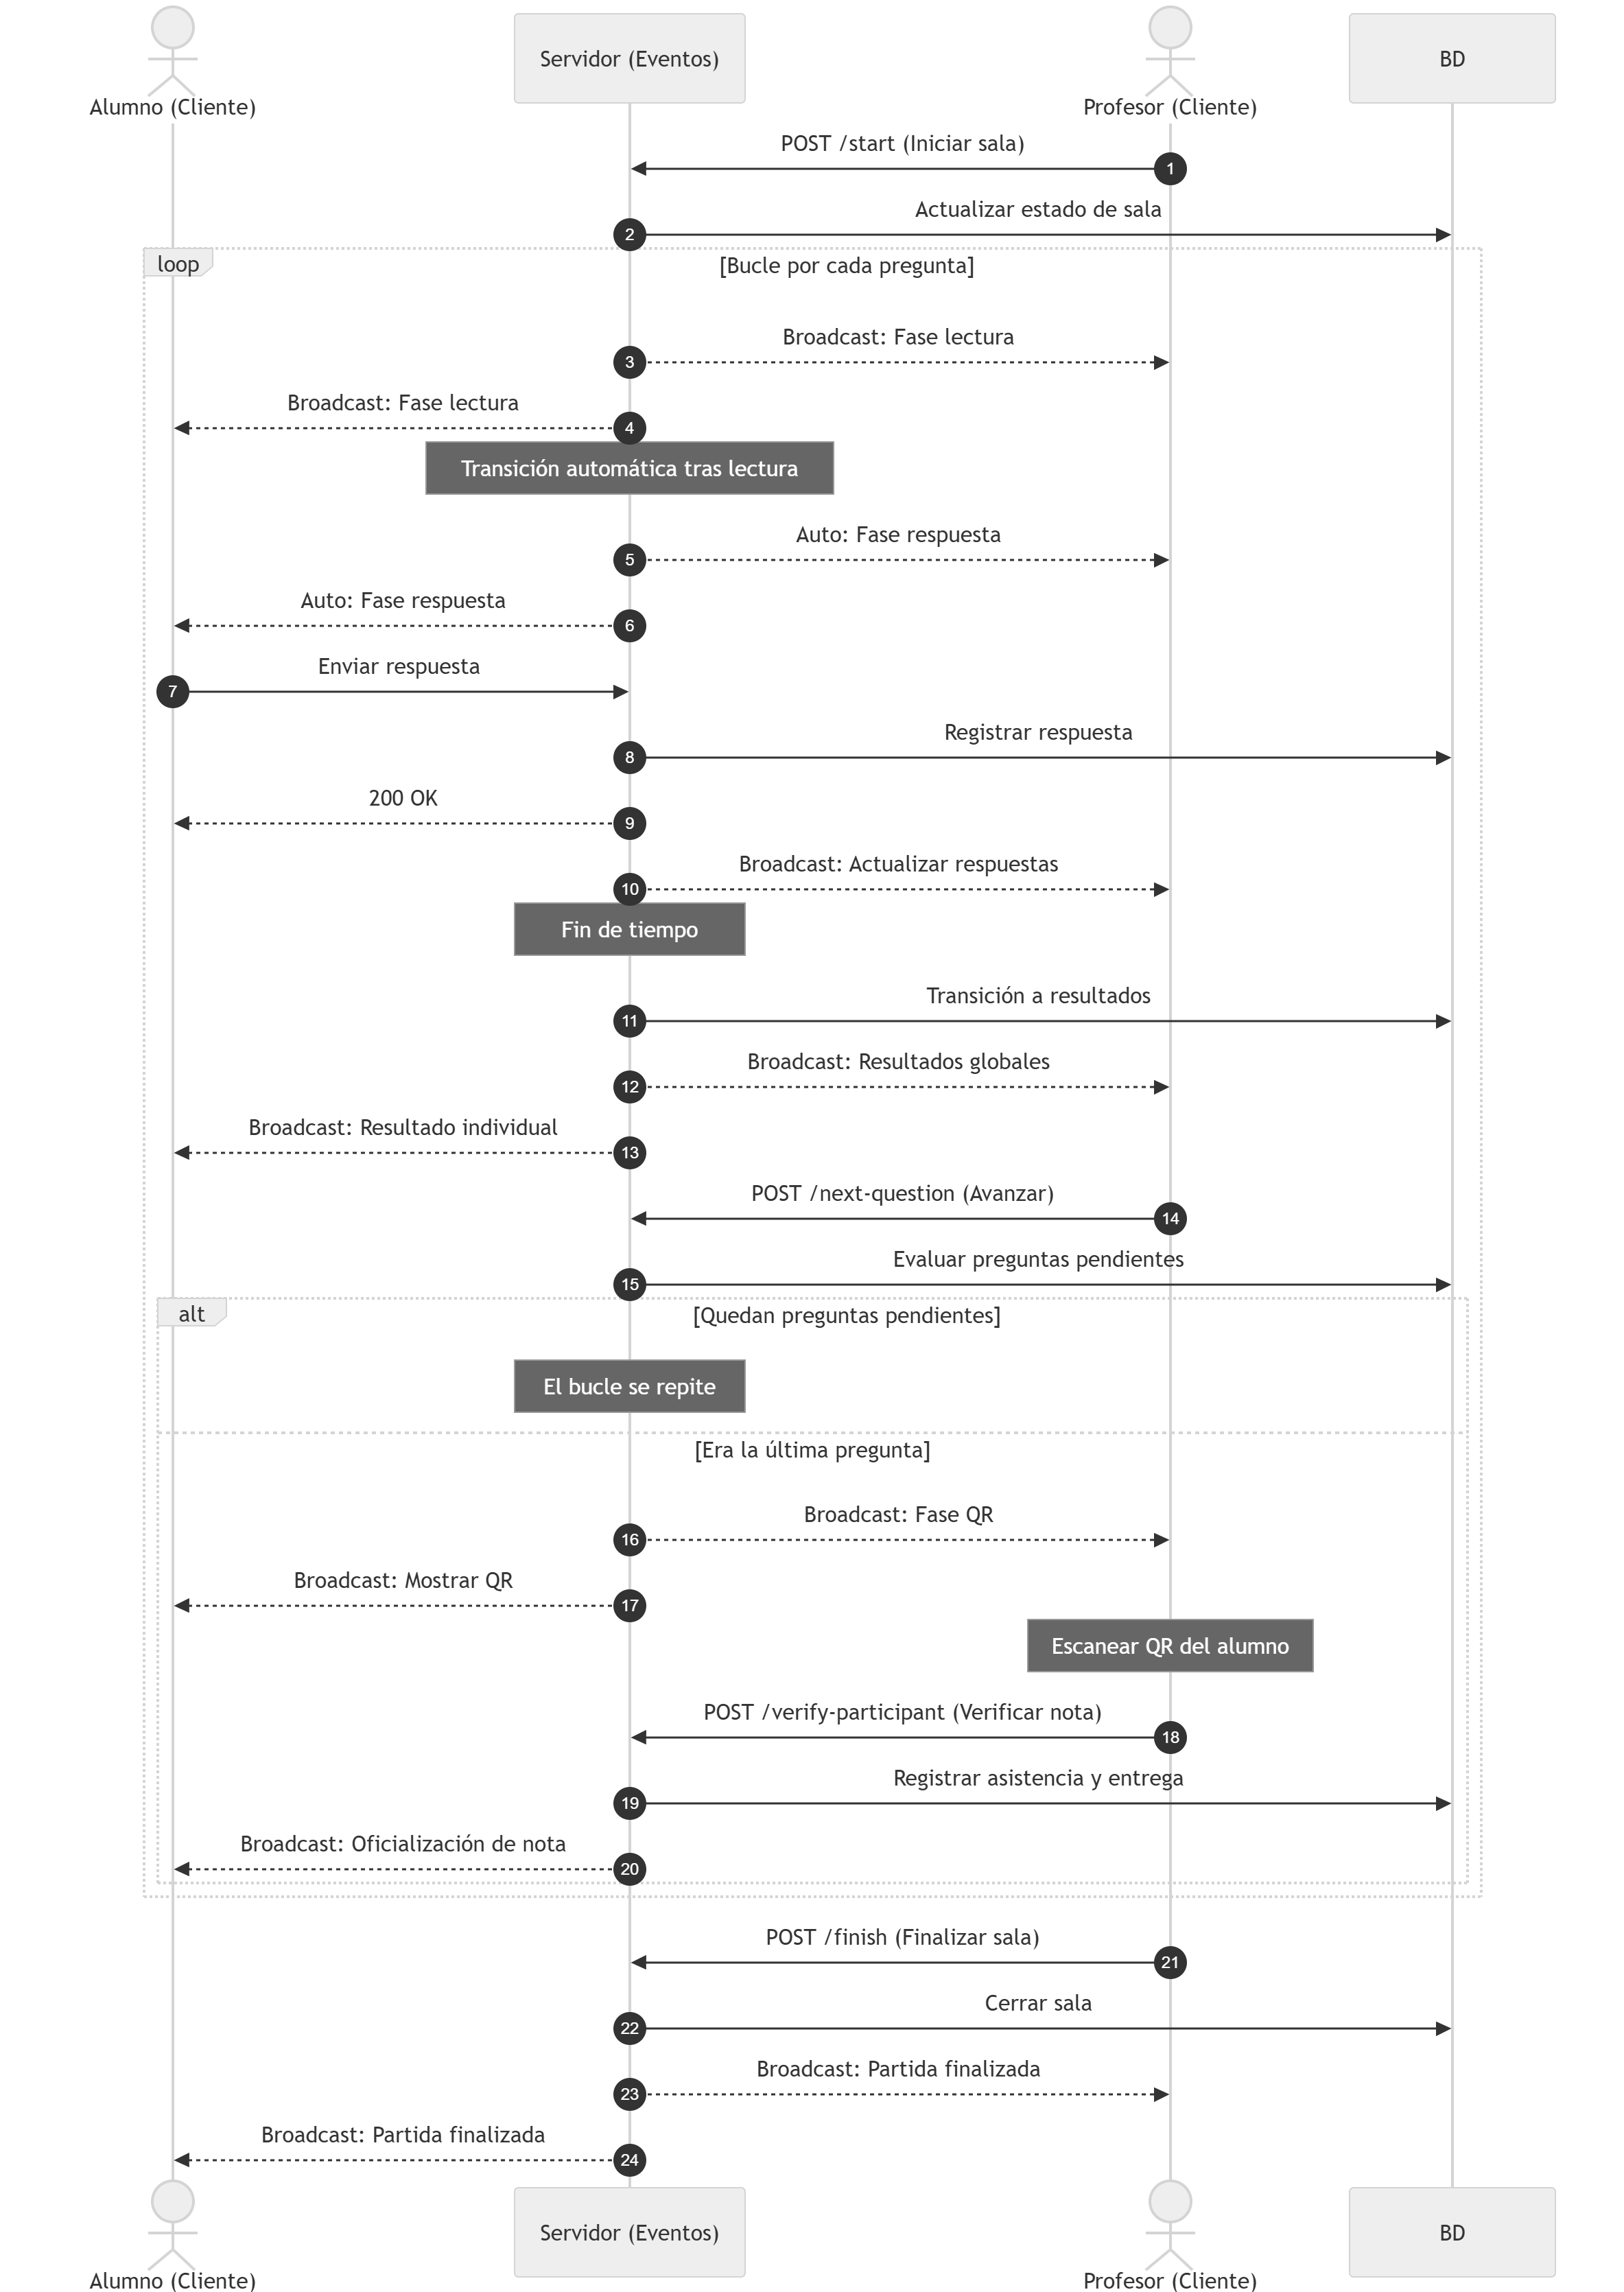
\includegraphics[width=1.06\textwidth]{figures/diagrama_secuencia_eventos.png}
    }
    \caption{Diagrama de secuencia de la transmisión de eventos en una sala.}
    \label{fig:diagrama_secuencia_eventos}
\end{figure}

\section{Arquitectura global del sistema}

La combinación de los tres patrones previamente descritos se consolida en una estructura global unificada. Como se ilustra en el \hyperref[fig:arquitectura_global]{esquema de la arquitectura global} del sistema, este enfoque permite integrar en un único marco de trabajo los terminales cliente, los canales de comunicación síncronos y asíncronos, las capas de servicios del \textit{backend} y el sistema de persistencia de datos.

\begin{figure}[H]
    \centering
    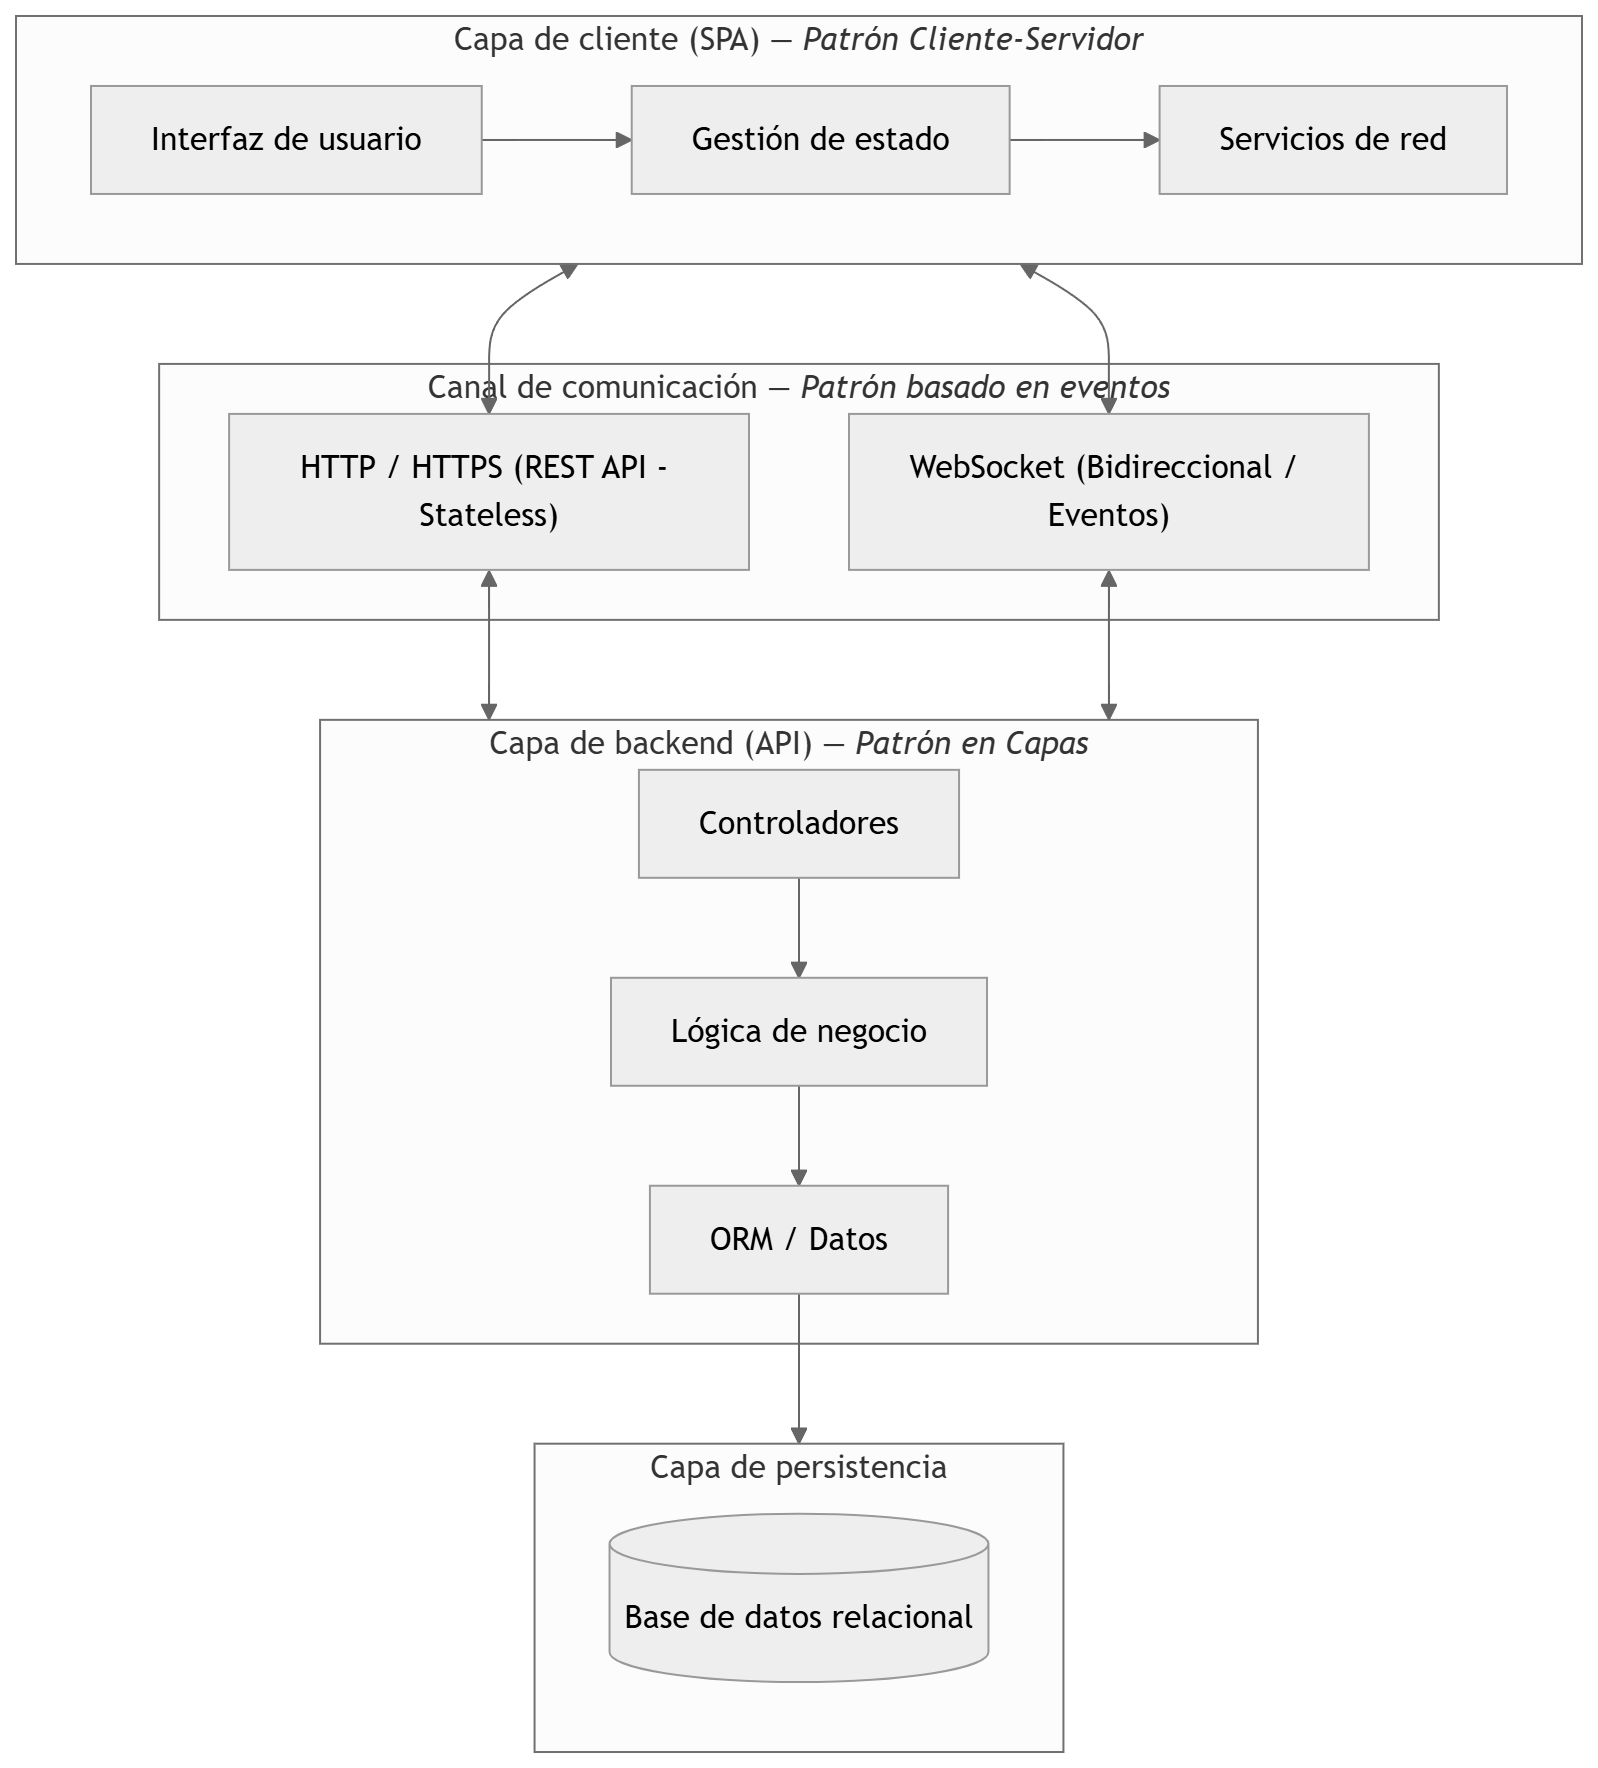
\includegraphics[width=0.85\textwidth]{figures/arquitectura_global.png}
    \caption{Esquema de la arquitectura global del sistema.}
    \label{fig:arquitectura_global}
\end{figure}

\section{Estructura modular del código}
Organización del proyecto en módulos independientes tanto para el Frontend (React) como para el Backend (FastAPI), facilitando la escalabilidad y el mantenimiento

Hablar de la organización del código en módulos independientes, explicando cómo se han estructurado y por qué es importante para la escalabilidad y el mantenimiento del proyecto.

\section{Modelo de datos}
Diagrama de dominio

Incluir el código mermaid y el diagrama

\section{Diseño de interfaces}
Mockups y resultado final

Mostrar los mockups iniciales y compararlos con el resultado final, explicando las decisiones de diseño tomadas y cómo se han implementado en la interfaz de usuario.

\section{Seguridad}
Autenticación JWT,  gestión de roles y tokens de verificación para participantes

\section{Documentación de la API}
Descripción de los endpoints principales de la API, detallando las peticiones, respuestas y la integración con el estándar OpenAPI

Aquí exprimiría el Swagger

    \chapter{Metodología técnica (CI/CD)}\label{cap:metodologia_tecnica}

Mi idea es haber explicado todas las herramientas en el capítulo 4, pero aquí se podría entrar más en detalle sobre cómo se han configurado y utilizado en lo que respecta a ci/cd, gestión de ramas, commits, etc. También se podrían incluir políticas de código, como pre-commits, hooks, plantillas de issues, etc. que no se hayan mencionado en capítulos anteriores.

\section{Políticas del repositorio}
Ramas, commits y versiones. Se puede mencionar los pre-commits, hooks, Github, Commitizen, Convenciones de commits, plantillas de issues, ... y su importancia en el desarrollo para trabajar de manera más organizada

\section{Integración y Despliegue Continuo (CI/CD)}
Descripción del ciclo ci/cd
\subsection{Configuración del Pipeline y automatización}
Implementación de flujos de trabajo en GitHub Actions y qué herramientas incluyen

\section{Perfiles de configuración y entornos}
Variables de entorno, secretos y configuración específica para los entornos de desarrollo, pruebas y producción.

\section{Métricas de calidad y análisis estático de código}
SonarCloud para el análisis estático de código, deuda técnica y cobertura de pruebas. (Para ello también habría que ver hasta qué punto se ha hablado de Sonar en capítulos anteriores)

Aqui quiero hacer especial énfasis para explicar la importancia de estas métricas, cómo se han configurado y qué resultados han dado, mostrando gráficas o ejemplos concretos de cómo han ayudado a mejorar la calidad del código y a identificar áreas de mejora.
También es importante recalcar que su uso es vital para evitar deuda técnica, y en el capítulo 9 de resultados diré que me arrepiento de haberlo implementado tan tarde y que me ha hecho tener que aplazar un par de issues que tenias planteadas para la entrega del tfg. (también podría ser en el capítulo de conclusiones)


    \chapter{Implementación y pruebas}\label{cap:implementacion_y_pruebas}

Una vez establecida la base arquitectónica y el diseño del sistema, corresponde abordar la materialización técnica de la plataforma, transformando los requisitos y decisiones de diseño arquitectónico previamente definidos en componentes funcionales de software. Para ello, en primer lugar se detallan los módulos críticos de la implementación tanto en el \textit{backend} como en el \textit{frontend}, haciendo especial énfasis en la sincronización en tiempo real y la seguridad. Posteriormente, se expone la estrategia integral de pruebas, los criterios de calidad adoptados y los resultados de cobertura obtenidos para garantizar la robustez del sistema.

\section{Componentes clave e implementación del sistema}\label{sec:componentes_clave}

En esta sección se exponen los aspectos más representativos del núcleo de \textit{Quizzie}, analizando las decisiones de diseño y patrones de software adoptados para dar respuesta a los requisitos funcionales más complejos: la comunicación bidireccional, la gestión del ciclo de vida de las salas y la seguridad del estado en el \textit{frontend}.

\subsection{Comunicación en tiempo real mediante WebSockets}\label{subsec:impl_websockets}

La interactividad en vivo entre el profesor y los alumnos requiere una arquitectura de baja latencia capaz de difundir eventos de forma simultánea a múltiples clientes mediante el protocolo WebSocket~\cite{websocket_protocol}.

\subsubsection{Gestor de conexiones en el backend (\texttt{ConnectionManager})}
En la ruta \texttt{backend/routers/stage.py}, el gestor de conexiones implementa una adaptación concurrente del patrón de diseño \textit{Observer}~\cite{gamma1994design} combinada con una arquitectura de publicación-suscripción (\textit{Pub-Sub})~\cite{eugster2003pubsub}, permitiendo registrar, desacoplar y administrar dinámicamente el ciclo de vida de las instancias activas de \texttt{WebSocket} asociadas a cada sala mediante su identificador único (\texttt{room\_id}).

\begin{figure}[H]
  \centering
  \makebox[\textwidth][c]{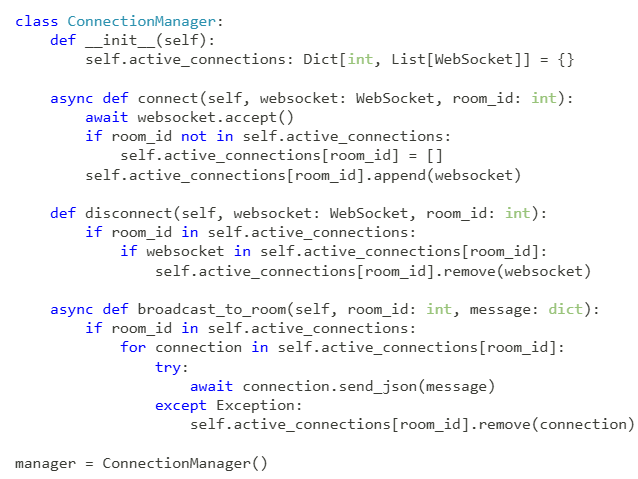
\includegraphics[width=0.9\textwidth]{listings/gestor_conexiones_backend.png}}
  \captionof{lstlisting}{Gestor de conexiones en el \textit{backend}}
  \label{lst:gestor_conexiones_backend}
\end{figure}

Esta estructura permite emitir mensajes masivos con formato JSON mediante el método \texttt{broadcast\_to\_room}. Asimismo, incluye un mecanismo de tolerancia a fallos en bloque \texttt{try-except} que elimina automáticamente las conexiones diferidas o corruptas sin interrumpir la emisión hacia el resto de los participantes.

\newpage

\subsubsection{Suscripción y recepción de eventos en el cliente React}
En el \textit{frontend}, el componente establece la conexión WebSocket con el servidor enviando el parámetro del rol (\texttt{teacher} o \texttt{student}) como parámetro de consulta.

\begin{figure}[H]
  \centering
  \makebox[\textwidth][c]{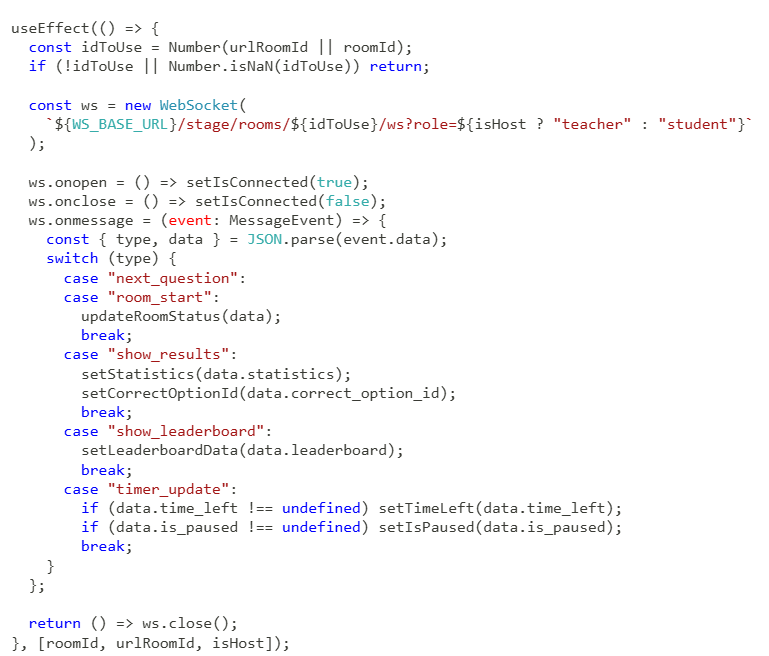
\includegraphics[width=1.1\textwidth]{listings/recepcion_eventos_react.png}}
  \captionof{lstlisting}{Conexión y enrutamiento de eventos WebSocket en React}
  \label{lst:recepcion_eventos_react}
\end{figure}

El \textit{handler} \texttt{onmessage} actúa como un enrutador de eventos de la interfaz de usuario, mutando el estado local de React en función del tipo de evento recibido. Asimismo, la función de retorno del \textit{hook} \texttt{useEffect} (\textit{cleanup function}) garantiza el cierre formal del socket al desmontar el componente, previniendo fugas de memoria.

\newpage

\subsection{Gestión de sala, estado, tiempo y aleatoriedad}\label{subsec:impl_state_time}

El correcto funcionamiento de las sesiones depende de mantener la sala sincronizada y lista para todos los usuarios. Para lograrlo, el servidor asume el control centralizado de los eventos y las decisiones críticas, gestionando el avance del estado de la sala y evitando depender del estado o el reloj individual de cada cliente.

\subsubsection{Cálculo determinista del tiempo restante en UTC}
En \texttt{backend/routers/stage.py}, la medición del tiempo no depende del reloj del cliente, sino de la diferencia estricta de marcas temporales en UTC.

\begin{figure}[H]
  \centering
  \makebox[\textwidth][c]{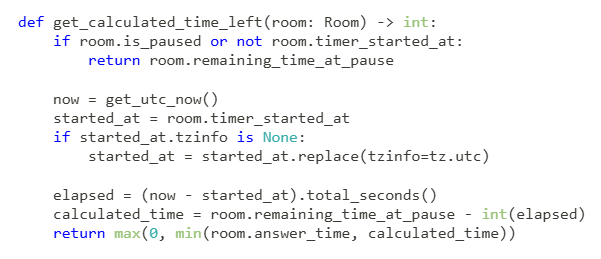
\includegraphics[width=0.9\textwidth]{listings/calculo_tiempo_utc.png}}
  \captionof{lstlisting}{Cálculo determinista del tiempo restante en el servidor}
  \label{lst:calculo_tiempo_utc}
\end{figure}

Al restar el instante actual (\texttt{get\_utc\_now()}) del momento de inicio (\texttt{timer\_started\_at}), el sistema inmuniza la cuenta atrás frente a retrasos de red o pausas de ejecución en el cliente.

\newpage

\subsubsection{Pausa automática por desconexión del profesor}
Para mitigar imprevistos técnicos durante una sesión presencial, el servidor detecta si la conexión WebSocket del docente cae inesperadamente.

\begin{figure}[H]
  \centering
  \makebox[\textwidth][c]{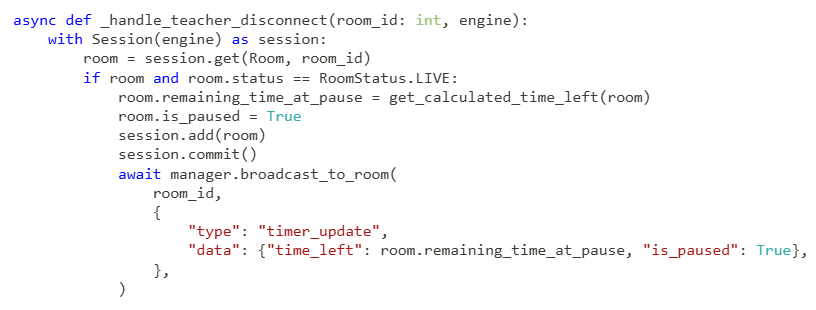
\includegraphics[width=1.1\textwidth]{listings/desconexion_profesor.png}}
  \captionof{lstlisting}{Gestión de desconexión imprevista del profesor}
  \label{lst:desconexion_profesor}
\end{figure}

La función congela la partida almacenando el tiempo restante exacto en \texttt{remaining\_time\_at\_pause} mediante \texttt{get\_calculated\_time\_left} y notifica inmediatamente a todos los estudiantes, pausando la interfaz hasta la reconexión del profesor.

\subsubsection{Barajado determinista de opciones}
Para evitar que los estudiantes copien observando la opción seleccionada en la pantalla de un compañero, el \textit{backend} desordena las opciones mediante una semilla \textit{hash}.

\begin{figure}[H]
  \centering
  \makebox[\textwidth][c]{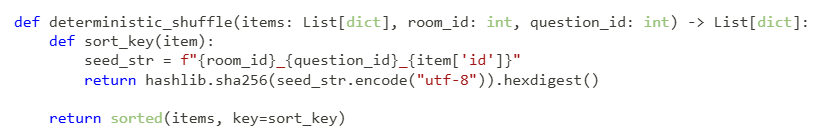
\includegraphics[width=1.1\textwidth]{listings/barajado_anticopia.png}}
  \captionof{lstlisting}{Algoritmo de barajado determinista anti-copia}
  \label{lst:barajado_anticopia}
\end{figure}

El algoritmo genera un \textit{hash SHA-256} combinando la sala, la pregunta y la opción. Esto altera la disposición de las respuestas para cada partida pero mantiene un orden idéntico si un alumno reconecta o recarga su cliente.

\subsubsection{Transición de preguntas y fase de verificación}
El endpoint \texttt{PATCH /rooms/:room\_id/next-question} coordina el avance del cuestionario o la transición a la fase final.

\begin{figure}[H]
  \centering
  \makebox[\textwidth][c]{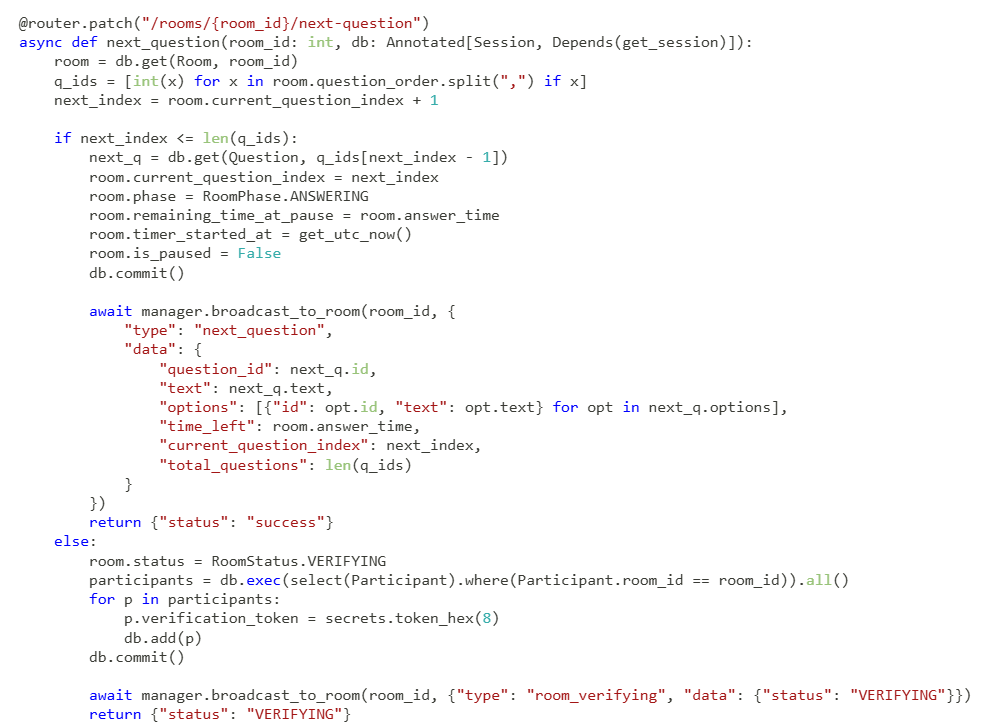
\includegraphics[width=1.2\textwidth]{listings/siguiente_pregunta_verificacion.png}}
  \captionof{lstlisting}{Avance de pregunta y paso a siguiente fase}
  \label{lst:siguiente_pregunta_verificacion}
\end{figure}

Si restan preguntas por responder, el controlador actualiza el índice y emite el evento correspondiente. Al agotar la batería de preguntas, la sala cambia al estado \texttt{VERIFYING} y genera tokens criptográficos efímeros mediante \texttt{secrets.token\_hex(8)}.

\newpage

\subsubsection{Verificación presencial mediante código QR}
Una vez concluida la partida, el resultado acumulado debe ser validado por el docente escaneando un código QR en el dispositivo del alumno.

\begin{figure}[H]
  \centering
  \makebox[\textwidth][c]{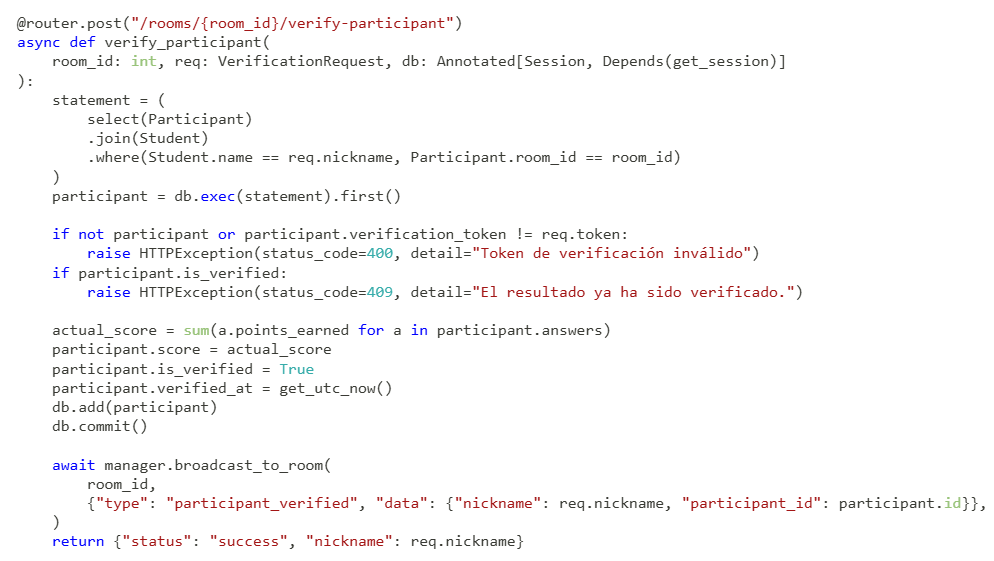
\includegraphics[width=1.2\textwidth]{listings/verificacion_presencial_qr.png}}
  \captionof{lstlisting}{Validación presencial del participante mediante token QR}
  \label{lst:verificacion_presencial_qr}
\end{figure}

El controlador valida el token efímero (\texttt{req.token}), recalcula la puntuación final sumando los puntos auditados, marca al participante como verificado y notifica la confirmación en tiempo real.

\newpage

\subsection{Seguridad, contexto y autenticación}\label{subsec:impl_security_context}

Este bloque aborda el tratamiento del estado del jugador, el saneamiento de datos en la SPA y la protección de endpoints sensibles mediante tokens JWT.

\subsubsection{Persistencia y saneamiento de estado en la SPA}
En \texttt{RoomContext} se encapsula la gestión de la sesión del jugador mediante la \textit{API Context} de React.

\begin{figure}[H]
  \centering
  \makebox[\textwidth][c]{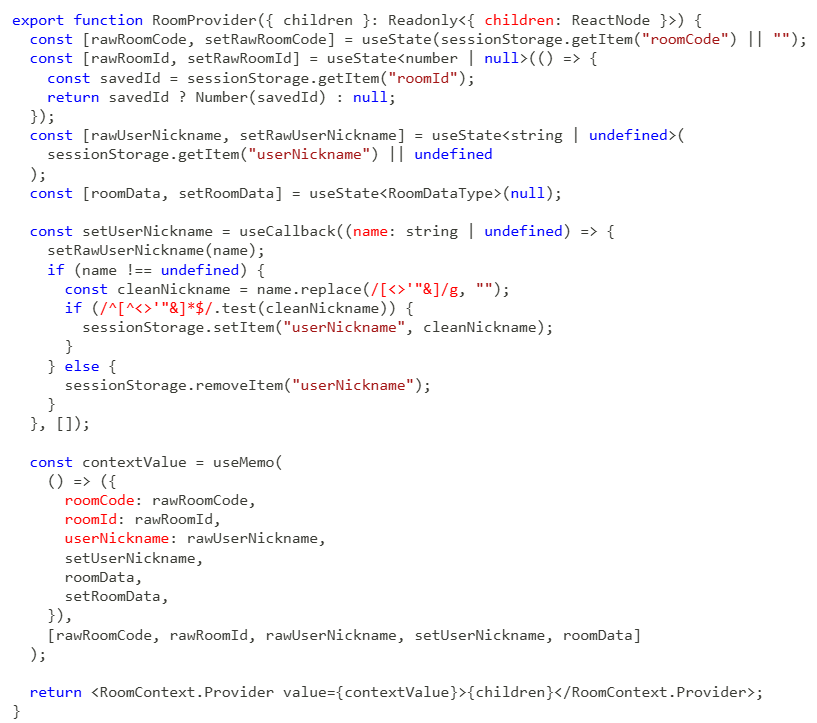
\includegraphics[width=1.05\textwidth]{listings/contexto_sala.png}}
  \captionof{lstlisting}{Gestión del contexto de la sala}
  \label{lst:contexto_sala}
\end{figure}

El componente recupera de forma síncrona los identificadores desde \texttt{sessionStorage} para garantizar la persistencia del estado frente a recargas accidentales del navegador. Asimismo, se aplica una función de saneamiento que purga caracteres sensibles (\texttt{<, >, ', ", \&}) antes de su persistencia y renderizado, mitigando vectores de ataque por inyección de scripts en sitios cruzados o XSS (\textit{Cross-Site Scripting}) \cite{owaspTop10, zalewski2011tangold}.

\subsubsection{Autenticación y protección de endpoints con JWT}
En \texttt{backend/auth.py}, se implementa un mecanismo de inyección de dependencias para autenticar las peticiones de los docentes mediante cabeceras HTTP.

\begin{figure}[H]
  \centering
  \makebox[\textwidth][c]{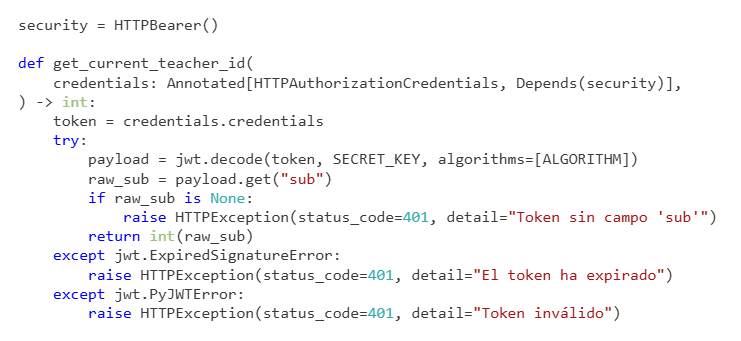
\includegraphics[width=1\textwidth]{listings/autenticacion_jwt_backend.png}}
  \captionof{lstlisting}{Inyección de dependencia para la validación de tokens JWT}
  \label{lst:autenticacion_jwt_backend}
\end{figure}

Esta función intercepta el \textit{Bearer token} emitido en las peticiones HTTP, descifra la firma criptográfica del estándar JSON Web Token~\cite{ietf_jwt_rfc7519} utilizando la clave secreta del servidor (\texttt{SECRET\_KEY}) y verifica su validez temporal antes de permitir el acceso a los controladores protegidos.


\section{Estrategia de testing}\label{sec:estrategia_testing}
Unitarias, integración, E2E, etc

Me gustaría mencionar también su importancia y los objetivos de cobertura que tengo, quizás lo mejor sea en este capítulo mencionar los umbrales objetivos y en el capítulo 9 de resultados hablar de su cumplimiento
\section{Casos de prueba y validación}\label{sec:casos_de_prueba_y_validacion}

Descripción de los casos de prueba utilizados para validar los criterios de aceptación y alcanzar la cobertura objetivo

\section{Pruebas de carga y rendimiento}
Descripción de las pruebas de carga y rendimiento realizadas

Importante porque los cuestionarios son en directo y con muchas personas simultáneamente

    \chapter{Resultados y evaluación}\label{cap:resultados_y_evaluacion}

Una vez finalizado el ciclo de desarrollo e implementadas las pruebas de verificación expuestas en el capítulo anterior, el presente capítulo aborda la auditoría cuantitativa y cualitativa del proyecto. A través de este análisis se evalúa el desempeño de la solución construida respecto a los compromisos definidos durante la fase de planificación, contrastando la ejecución real frente a las líneas base establecidas. Asimismo, se documenta la gestión de cambios articulada durante el desarrollo, la resolución efectiva de las pruebas y una retrospectiva técnica en torno a la infraestructura de integración continua y métricas de calidad de código.
 
\section{Cumplimiento de la Línea Base del Alcance}\label{sec:cumplimiento_alcance}

La \hyperref[sec:linea_base_del_alcance]{Línea Base del Alcance} quedó formalizada en la \hyperref[cap:gestion_del_proyecto]{planificación del proyecto} a través de la \hyperref[subsec:edt]{EDT} y su correspondiente \hyperref[subsec:diccionario_edt]{diccionario}, distribuyendo el esfuerzo en cuatro paquetes troncales: Gestión del proyecto, Diseño y arquitectura, Producto software y Documentación final. 

A nivel global del proyecto, los entregables documentales, de gestión y de diseño preliminar se han completado al \textbf{100\%}, quedando consolidados a lo largo de los capítulos técnicos, anexos y código fuente de esta memoria. Por su parte, el paquete \textbf{Producto software} materializa con éxito el flujo íntegro del sistema a través de las tres \textit{releases} planificadas; no obstante, al haberse pospuesto dos de los doce objetivos funcionales contemplados en el diseño inicial, el grado de consecución de dichos objetivos se sitúa en el \textbf{83{,}33\%}.

Para auditar las desviaciones del alcance del sistema, el siguiente cuadro detalla en primer término los dos objetivos funcionales que resultaron formalmente pospuestos, justificando el motivo de su aplazamiento:

\begin{table}[H]
\centering
\normalsize
\renewcommand{\arraystretch}{1.5}
\makebox[\textwidth][c]{%
\begin{tabular}{llp{10.7cm}}
\hline
\textbf{ID} & \textbf{Objetivo funcional} & \textbf{Motivo del aplazamiento} \\ \hline
\hyperref[obj:09]{OBJ-09} & Asistente IA & Evitar la dependencia de cuotas de facturación por consumo de \textit{tokens}, límites de tasa (\textit{rate limits}) y sobrecostes imprevistos de servicios externos, priorizando un núcleo completamente autosuficiente. \\ 
\hyperref[obj:11]{OBJ-11} & Gestión de grupos & Elevado coste de oportunidad: el gran esfuerzo temporal necesario para su implementación no justificaba el valor añadido, decidiendo concentrar ese tiempo en consolidar la concurrencia y la estabilidad de las salas en vivo. \\ \hline
\end{tabular}%
}
\caption{Objetivos funcionales pospuestos.}
\label{tab:objetivos_pospuestos}
\end{table}

Gracias a las relaciones establecidas en la \hyperref[tab:matriz_trazabilidad]{matriz de trazabilidad unificada}, es posible determinar con precisión cómo repercute la postergación de estos dos objetivos en los casos de uso, historias de usuario y requisitos funcionales asociados:

\begin{itemize}
    \item \textbf{Asistente de IA (\hyperref[obj:09]{OBJ-09}):} Conlleva la postergación completa del caso de uso \textbf{\hyperref[cu:03]{CU-03} - Generar preguntas con IA} y de la historia de usuario \textbf{\hyperref[hu:pr-09]{HU-PR-09} - Generación asistida de preguntas}, afectando a cuatro requisitos funcionales. Estos requisitos han quedado formalizados en el repositorio del proyecto como líneas de evolución futura:

\begin{table}[H]
\centering
\normalsize
\renewcommand{\arraystretch}{1.5}

\makebox[\textwidth][c]{%
\begin{tabular}{llc}
\hline
\textbf{ID} & \textbf{Requisito funcional} & \textbf{GitHub Issue} \\ \hline
\hyperref[req:34]{RF-34} & Generación preguntas & \issue{95}  \\
\hyperref[req:35]{RF-35} & Asistente de ayuda &  \issue{96} \\
\hyperref[req:36]{RF-36} & Navegación y tutorial por IA & \issue{97} \\
\hyperref[req:37]{RF-37} & Revisión post IA & \issue{98} \\ \hline
\end{tabular}%
}
\caption{Requisitos funcionales pospuestos para OBJ-09.}
\label{tab:rf_pospuestos_obj09}
\end{table}

    \item \textbf{Gestión de grupos (\hyperref[obj:11]{OBJ-11}):} Implica posponer íntegramente el caso de uso \textbf{\hyperref[cu:11]{CU-11} - Gestionar grupos} y la historia de usuario \textbf{\hyperref[hu:pr-07]{HU-PR-07} - Organización por grupos de clase}, afectando a un único requisito funcional:
\begin{table}[H]
\centering
\normalsize
\renewcommand{\arraystretch}{1.5}
\makebox[\textwidth][c]{%
\begin{tabular}{llc}
\hline
\textbf{ID} & \textbf{Requisito funcional} & \textbf{GitHub Issue} \\ \hline
\hyperref[req:38]{RF-38} & Crear clase & \issue{99} \\ \hline
\end{tabular}%
}
\caption{Requisito funcional pospuesto para OBJ-11.}
\label{tab:rf_pospuestos_grupos}
\end{table}

\end{itemize}

Por otro lado, los diez objetivos funcionales restantes alcanzaron cobertura operativa suficiente para la entrega. La siguiente tabla resume la retrospectiva técnica, los desafíos de diseño y las decisiones clave adoptadas durante su materialización:

\begin{table}[H]
\centering
\normalsize
\renewcommand{\arraystretch}{1.5}
\makebox[\textwidth][c]{%
\begin{tabular}{lp{3.7cm}p{10.7cm}}
\hline
\textbf{ID} & \textbf{Objetivo funcional} & \textbf{Retrospectiva técnica e impacto en el desarrollo} \\ \hline
\hyperref[obj:01]{OBJ-01} & Módulo de usuario y autenticación & Implementación sólida de JWT y Bcrypt. Para evitar bloqueos en el hilo principal de la API por la latencia del servidor SMTP de Gmail, el envío del código de verificación por correo se delegó a tareas en segundo plano. \\ 
\hyperref[obj:02]{OBJ-02} & Gestión de cuestionarios & Se optó por borrado lógico (\textit{soft delete}) en cascada para impedir que la edición o eliminación de preguntas corrompiera los registros de salas históricas. \\ 
\hyperref[obj:03]{OBJ-03} & Creación de salas & Se implementó una máquina de estados en el servidor para controlar las fases de la partida, garantizando un flujo sincronizado y previniendo saltos de estado indebidos. \\ 
\hyperref[obj:04]{OBJ-04} & Acceso rápido & Entrada ágil e inmediata sin necesidad de registro previo. Para evitar que un refresco accidental del navegador expulsara al estudiante de la partida, la sesión activa se conservó localmente mediante \texttt{sessionStorage}. \\ 
\hyperref[obj:05]{OBJ-05} & Interacción en tiempo real & La recepción de respuestas se gestionó en memoria garantizando que cada participante emitiera un único voto por pregunta. Además, se centralizó el temporizador en el servidor para anular intentos de manipulación o ventajas por desajustes horarios entre los clientes. \\ 
\hyperref[obj:06]{OBJ-06} & Verificación QR & Generación distribuida en el cliente para liberar de procesamiento al servidor mediante la librería \texttt{qrcode.react}. La carga útil del código QR estructura un objeto JSON con los datos clave de la evaluación (UVUS, sala y puntuación), acompañado de un token criptográfico de un solo uso. \\ 
\hyperref[obj:07]{OBJ-07} & Persistencia validada & Se logró el desacoplamiento entre el estado efímero de la partida y el almacenamiento persistente: solo los resultados verificados se consolidan en la base de datos. \\  
\hyperref[obj:08]{OBJ-08} & Estadísticas y análisis & Agregación reactiva en memoria al cierre de cada ronda para computar la distribución de respuestas, aciertos globales y el podio en tiempo real, evitando sobrecargar la base de datos con consultas recurrentes. \\  
\hyperref[obj:10]{OBJ-10} & Escaneo de código QR & Lectura ágil mediante \texttt{html5-qrcode} con solicitud de permisos de cámara, validando el \textit{token} criptográfico contra el servidor en un solo paso atómico. \\  
\hyperref[obj:12]{OBJ-12} & Exportación de datos & Se habilitó la descarga de resultados en formato CSV, garantizando la compatibilidad con hojas de cálculo. \\  \hline
\end{tabular}%
}
\caption{Retrospectiva técnica de los objetivos funcionales.}
\label{tab:objetivos_completados}
\end{table}

\newpage

Cabe destacar que los nueve casos de uso y dieciséis historias de usuario que sustentan estos diez objetivos están plenamente disponibles en sus flujos troncales. Sin embargo, para cumplir con el calendario fijado sin comprometer la estabilidad, se decidió catalogar como mejoras o extensiones secundarias siete requisitos funcionales. La siguiente tabla detalla estos requisitos de ampliación y las \textit{issues} abiertas para su integración en versiones sucesivas:

\begin{table}[H]
\centering
\normalsize
\renewcommand{\arraystretch}{1.5}
\makebox[\textwidth][c]{%
\begin{tabular}{llc}
\hline
\textbf{ID} & \textbf{Requisito funcional} & \textbf{GitHub Issue} \\ \hline
\hyperref[req:12]{RF-12} & Importación & \issue{100} \\
\hyperref[req:32]{RF-32} & Listado en vivo & \issue{101} \\
\hyperref[req:33]{RF-33} & Estadísticas & \issue{102} \\
\hyperref[req:42]{RF-42} & Bonificación por tiempo & \issue{103} \\
\hyperref[req:43]{RF-43} & Sistema de rachas & \issue{104} \\
\hyperref[req:44]{RF-44} & Configuración de puntuación & \issue{105} \\
\hyperref[req:46]{RF-46} & Creación/edición avanzada & \issue{106} \\ \hline
\end{tabular}%
}
\caption{Requisitos funcionales pospuestos como puntos de extensión.}
\label{tab:rf_mejoras_issues}
\end{table}

En términos cuantitativos, este ajuste de alcance deliberado se traduce en que 9 de los 11 casos de uso diseñados (\textbf{81{,}82\,\%}) y 16 de las 18 historias de usuario (\textbf{88{,}89\,\%}) se encuentran plenamente operativos en sus flujos de valor principal. En el nivel de especificación atómica, 35 de los 47 requisitos funcionales (\textbf{74{,}47\,\%}) han sido implementados y verificados con éxito, garantizando la totalidad de la operativa requerida en el aula presencial y dejando acotadas las extensiones como trabajo futuro.

\section{Tiempo real frente a Línea Base del Cronograma}\label{sec:tiempo_real_vs_cronograma}

Para auditar el desempeño temporal del proyecto frente a la \hyperref[sec:linea_base_del_cronograma]{Línea Base del Cronograma}, se ha consolidado el registro continuo de dedicación temporal a través de Clockify, cuyo informe detallado queda recogido íntegramente en el \hyperref[anexo:clockify]{anexo de dedicación temporal}. Las horas se han computado a nivel de tareas operativas individuales, asignando en la herramienta una etiqueta (\textit{tag}) que las vincula directamente con su actividad homóloga más próxima de la planificación inicial. Este mecanismo permite clasificar el esfuerzo según el rol profesional desempeñado, trazabilidad que se empleará más adelante en la \hyperref[tab:horas_roles_previstas_reales]{tabla de dedicación por roles} para calcular las desviaciones en los gastos de contratación.

\textcolor{red}{\textbf{[TODO: Actualizar informe cuando estén todas las horas computadas]}}

El siguiente cuadro resume la comparativa entre la estimación inicial y la dedicación real registrada por fase de trabajo:

\textcolor{red}{\textbf{[TODO: Rellenar las horas]}}

\begin{table}[H]
\centering
\small
\renewcommand{\arraystretch}{1.3}
\begin{tabular}{llcc}
\hline
\textbf{ID} & \textbf{Fase} & \textbf{Horas previstas} & \textbf{Horas reales} \\ \hline
F-01 & Planificación & 20 h & 11 h \\
F-02 & Documentación & 20 h & 27,14 h \\
F-03 & Inicio        & 11 h & 12,50 h \\
F-04 & CI/CD         & 17 h & 19,87 h \\
F-05 & MVP           & 65 h & 55,40 h \\
F-06 & Testing       & 15 h & 42,74 h \\
F-07 & Core          & 49 h & 45,24 h \\
F-08 & QA            & 13 h & 23,73 h \\
F-09 & Memoria       & 70 h &   \\
F-10 & Defensa       & 20 h &  \\ \hline
\multicolumn{2}{l}{\textbf{Total}} & \textbf{300 h} &   \\ \hline
\end{tabular}
\caption{Comparativa de horas previstas y reales por fase del proyecto.}
\label{tab:horas_fases_previstas_reales}
\end{table}

\textcolor{red}{\textbf{[TODO: Redactar retrospectiva general de desviaciones temporales una vez cerrado el cómputo final de horas en Clockify]}}

Este incremento en el esfuerzo dedicado a la robustez técnica y las pruebas del sistema impactó de forma directa en los plazos globales. Si bien la planificación inicial contemplaba finalizar el proyecto para la convocatoria ordinaria de junio, mantener dicha fecha habría obligado a comprometer la calidad del producto o recortar el rigor de la memoria técnica. Por ello, se optó formalmente por trasladar la finalización y defensa a la convocatoria extraordinaria de octubre, quedando esta modificación justificada y registrada en la sección de \hyperref[sec:desviaciones_y_gestion_cambios]{gestión de cambios}.

A continuación, se muestra una comparativa entre la Línea Base del Cronograma y la ejecución real, representada mediante un diagrama de Gantt:

\begin{figure}[H]
\centering
\noindent\makebox[\textwidth][c]{%
\begin{ganttchart}[
    hgrid=false, 
    vgrid=false, 
    x unit=0.0636cm,
    y unit title=0.55cm,
    y unit chart=0.72cm, 
    time slot format=isodate,
    inline,
    title label font=\scriptsize\bfseries,
    title calendar link/.style={draw=black},
    canvas/.style={draw=black, fill=white}
]{2026-01-15}{2026-10-17}

    \gantttitle{Ene}{17}
    \gantttitle{Feb}{28}
    \gantttitle{Mar}{31}
    \gantttitle{Abr}{30}
    \gantttitle{May}{31}
    \gantttitle{Jun}{30}
    \gantttitle{Jul}{31}
    \gantttitle{Ago}{31}
    \gantttitle{Sep}{30}
    \gantttitle{Oct}{17} \\

    % F01 
    \ganttbar[bar/.style={fill=gray!45, draw=primaryMagenta, line width=0.5pt, rounded corners=1pt}, bar height=0.40, bar top shift=0.08, bar label font=\tiny\bfseries\color{black!80}, ganttbar label node/.append style={xshift=0.35cm}]{F01-Plan}{2026-01-15}{2026-01-28}
    \ganttbar[bar/.style={fill=primaryMagenta, draw=primaryMagenta, rounded corners=1pt}, bar height=0.40, bar top shift=0.48, bar label font=\tiny\bfseries\color{white}, ganttbar label node/.append style={xshift=0.15cm}]{F01}{2026-01-15}{2026-01-26} \\

    % F02  
    \ganttbar[bar/.style={fill=gray!45, draw=secondaryMagenta, line width=0.5pt, rounded corners=1pt}, bar height=0.40, bar top shift=0.08, bar label font=\tiny\bfseries\color{black!80}]{F02-Plan}{2026-01-29}{2026-04-14}
    \ganttbar[bar/.style={fill=secondaryMagenta, draw=secondaryMagenta, rounded corners=1pt}, bar height=0.40, bar top shift=0.48, bar label font=\tiny\bfseries\color{white}]{F02}{2026-01-26}{2026-06-07} \\

    % F03 
    \ganttbar[bar/.style={fill=gray!45, draw=primaryMagenta, line width=0.5pt, rounded corners=1pt}, bar height=0.40, bar top shift=0.08, bar label font=\tiny\bfseries\color{black!80}]{F03-Plan}{2026-01-29}{2026-02-11}
    \ganttbar[bar/.style={fill=primaryMagenta, draw=primaryMagenta, rounded corners=1pt}, bar height=0.40, bar top shift=0.48, bar label font=\tiny\bfseries\color{white}]{F03}{2026-01-30}{2026-02-09} \\

    % F04  
    \ganttbar[bar/.style={fill=gray!45, draw=secondaryCyan, line width=0.5pt, rounded corners=1pt}, bar height=0.40, bar top shift=0.08, bar label font=\tiny\bfseries\color{black!80}]{F04-Plan}{2026-02-12}{2026-04-26}
    \ganttbar[bar/.style={fill=secondaryCyan, draw=secondaryCyan, rounded corners=1pt}, bar height=0.40, bar top shift=0.48, bar label font=\tiny\bfseries\color{white}]{F04}{2026-02-11}{2026-08-14} \\

    % F05  
    \ganttbar[bar/.style={fill=gray!45, draw=primaryCyan, line width=0.5pt, rounded corners=1pt}, bar height=0.40, bar top shift=0.08, bar label font=\tiny\bfseries\color{black!80}]{F05-Plan}{2026-02-19}{2026-03-08}
    \ganttbar[bar/.style={fill=primaryCyan, draw=primaryCyan, rounded corners=1pt}, bar height=0.40, bar top shift=0.48, bar label font=\tiny\bfseries\color{white}]{F05}{2026-02-12}{2026-04-04} \\

    % F06 
    \ganttbar[bar/.style={fill=gray!45, draw=secondaryCyan, line width=0.5pt, rounded corners=1pt}, bar height=0.40, bar top shift=0.08, bar label font=\tiny\bfseries\color{black!80}]{F06-Plan}{2026-02-24}{2026-04-26}
    \ganttbar[bar/.style={fill=secondaryCyan, draw=secondaryCyan, rounded corners=1pt}, bar height=0.40, bar top shift=0.48, bar label font=\tiny\bfseries\color{white}]{F06}{2026-04-06}{2026-08-14} \\

    % F07 
    \ganttbar[bar/.style={fill=gray!45, draw=primaryCyan, line width=0.5pt, rounded corners=1pt}, bar height=0.40, bar top shift=0.08, bar label font=\tiny\bfseries\color{black!80}]{F07-Plan}{2026-03-09}{2026-04-12}
    \ganttbar[bar/.style={fill=primaryCyan, draw=primaryCyan, rounded corners=1pt}, bar height=0.40, bar top shift=0.48, bar label font=\tiny\bfseries\color{white}]{F07}{2026-04-15}{2026-04-28} \\

    % F08 
    \ganttbar[bar/.style={fill=gray!45, draw=primaryCyan, line width=0.5pt, rounded corners=1pt}, bar height=0.40, bar top shift=0.08, bar label font=\tiny\bfseries\color{black!80}]{F08-Plan}{2026-04-13}{2026-04-24}
    \ganttbar[bar/.style={fill=primaryCyan, draw=primaryCyan, rounded corners=1pt}, bar height=0.40, bar top shift=0.48, bar label font=\tiny\bfseries\color{white}]{F08}{2026-04-28}{2026-07-23} \\

    % F09 
    \ganttbar[bar/.style={fill=gray!45, draw=secondaryMagenta, line width=0.5pt, rounded corners=1pt}, bar height=0.40, bar top shift=0.08, bar label font=\tiny\bfseries\color{black!80}]{F09-Plan}{2026-04-15}{2026-05-17}
    \ganttbar[bar/.style={fill=secondaryMagenta, draw=secondaryMagenta, rounded corners=1pt}, bar height=0.40, bar top shift=0.48, bar label font=\tiny\bfseries\color{white}]{F09}{2026-05-04}{2026-10-17} \\

    % F10 
    \ganttbar[bar/.style={fill=gray!45, draw=secondaryMagenta, line width=0.5pt, rounded corners=1pt}, bar height=0.40, bar top shift=0.08, bar label font=\tiny\bfseries\color{black!80}]{F10-Plan}{2026-05-18}{2026-06-12}
    \ganttbar[bar/.style={fill=secondaryMagenta, draw=secondaryMagenta, rounded corners=1pt}, bar height=0.40, bar top shift=0.48, bar label font=\tiny\bfseries\color{white}]{F10}{2026-10-01}{2026-10-17}

    % Líneas semanales 
    \ganttvrule[vrule/.style={draw=gray!60, dotted, line width=0.4pt}, vrule label node/.style={anchor=south, yshift=7.22cm, font=\tiny\bfseries\color{gray!80!black}, fill=white, inner sep=0.5pt}]{19}{2026-01-19}
    \ganttvrule[vrule/.style={draw=gray!60, dotted, line width=0.4pt}, vrule label node/.style={anchor=south, yshift=7.22cm, font=\tiny\bfseries\color{gray!80!black}, fill=white, inner sep=0.5pt}]{26}{2026-01-26}
    \ganttvrule[vrule/.style={draw=gray!60, dotted, line width=0.4pt}, vrule label node/.style={anchor=south, yshift=7.22cm, font=\tiny\bfseries\color{gray!80!black}, fill=white, inner sep=0.5pt}]{02}{2026-02-02}
    \ganttvrule[vrule/.style={draw=gray!60, dotted, line width=0.4pt}, vrule label node/.style={anchor=south, yshift=7.22cm, font=\tiny\bfseries\color{gray!80!black}, fill=white, inner sep=0.5pt}]{09}{2026-02-09}
    \ganttvrule[vrule/.style={draw=gray!60, dotted, line width=0.4pt}, vrule label node/.style={anchor=south, yshift=7.22cm, font=\tiny\bfseries\color{gray!80!black}, fill=white, inner sep=0.5pt}]{16}{2026-02-16}
    \ganttvrule[vrule/.style={draw=gray!60, dotted, line width=0.4pt}, vrule label node/.style={anchor=south, yshift=7.22cm, font=\tiny\bfseries\color{gray!80!black}, fill=white, inner sep=0.5pt}]{23}{2026-02-23}
    \ganttvrule[vrule/.style={draw=gray!60, dotted, line width=0.4pt}, vrule label node/.style={anchor=south, yshift=7.22cm, font=\tiny\bfseries\color{gray!80!black}, fill=white, inner sep=0.5pt}]{02}{2026-03-02}
    \ganttvrule[vrule/.style={draw=gray!60, dotted, line width=0.4pt}, vrule label node/.style={anchor=south, yshift=7.22cm, font=\tiny\bfseries\color{gray!80!black}, fill=white, inner sep=0.5pt}]{09}{2026-03-09}
    \ganttvrule[vrule/.style={draw=gray!60, dotted, line width=0.4pt}, vrule label node/.style={anchor=south, yshift=7.22cm, font=\tiny\bfseries\color{gray!80!black}, fill=white, inner sep=0.5pt}]{16}{2026-03-16}
    \ganttvrule[vrule/.style={draw=gray!60, dotted, line width=0.4pt}, vrule label node/.style={anchor=south, yshift=7.22cm, font=\tiny\bfseries\color{gray!80!black}, fill=white, inner sep=0.5pt}]{23}{2026-03-23}
    \ganttvrule[vrule/.style={draw=gray!60, dotted, line width=0.4pt}, vrule label node/.style={anchor=south, yshift=7.22cm, font=\tiny\bfseries\color{gray!80!black}, fill=white, inner sep=0.5pt}]{30}{2026-03-30}
    \ganttvrule[vrule/.style={draw=gray!60, dotted, line width=0.4pt}, vrule label node/.style={anchor=south, yshift=7.22cm, font=\tiny\bfseries\color{gray!80!black}, fill=white, inner sep=0.5pt}]{06}{2026-04-06}
    \ganttvrule[vrule/.style={draw=gray!60, dotted, line width=0.4pt}, vrule label node/.style={anchor=south, yshift=7.22cm, font=\tiny\bfseries\color{gray!80!black}, fill=white, inner sep=0.5pt}]{13}{2026-04-13}
    \ganttvrule[vrule/.style={draw=gray!60, dotted, line width=0.4pt}, vrule label node/.style={anchor=south, yshift=7.22cm, font=\tiny\bfseries\color{gray!80!black}, fill=white, inner sep=0.5pt}]{20}{2026-04-20}
    \ganttvrule[vrule/.style={draw=gray!60, dotted, line width=0.4pt}, vrule label node/.style={anchor=south, yshift=7.22cm, font=\tiny\bfseries\color{gray!80!black}, fill=white, inner sep=0.5pt}]{27}{2026-04-27}
    \ganttvrule[vrule/.style={draw=gray!60, dotted, line width=0.4pt}, vrule label node/.style={anchor=south, yshift=7.22cm, font=\tiny\bfseries\color{gray!80!black}, fill=white, inner sep=0.5pt}]{04}{2026-05-04}
    \ganttvrule[vrule/.style={draw=gray!60, dotted, line width=0.4pt}, vrule label node/.style={anchor=south, yshift=7.22cm, font=\tiny\bfseries\color{gray!80!black}, fill=white, inner sep=0.5pt}]{11}{2026-05-11}
    \ganttvrule[vrule/.style={draw=gray!60, dotted, line width=0.4pt}, vrule label node/.style={anchor=south, yshift=7.22cm, font=\tiny\bfseries\color{gray!80!black}, fill=white, inner sep=0.5pt}]{18}{2026-05-18}
    \ganttvrule[vrule/.style={draw=gray!60, dotted, line width=0.4pt}, vrule label node/.style={anchor=south, yshift=7.22cm, font=\tiny\bfseries\color{gray!80!black}, fill=white, inner sep=0.5pt}]{25}{2026-05-25}
    \ganttvrule[vrule/.style={draw=gray!60, dotted, line width=0.4pt}, vrule label node/.style={anchor=south, yshift=7.22cm, font=\tiny\bfseries\color{gray!80!black}, fill=white, inner sep=0.5pt}]{01}{2026-06-01}
    \ganttvrule[vrule/.style={draw=gray!60, dotted, line width=0.4pt}, vrule label node/.style={anchor=south, yshift=7.22cm, font=\tiny\bfseries\color{gray!80!black}, fill=white, inner sep=0.5pt}]{08}{2026-06-08}
    \ganttvrule[vrule/.style={draw=gray!60, dotted, line width=0.4pt}, vrule label node/.style={anchor=south, yshift=7.22cm, font=\tiny\bfseries\color{gray!80!black}, fill=white, inner sep=0.5pt}]{15}{2026-06-15}
    \ganttvrule[vrule/.style={draw=gray!60, dotted, line width=0.4pt}, vrule label node/.style={anchor=south, yshift=7.22cm, font=\tiny\bfseries\color{gray!80!black}, fill=white, inner sep=0.5pt}]{22}{2026-06-22}
    \ganttvrule[vrule/.style={draw=gray!60, dotted, line width=0.4pt}, vrule label node/.style={anchor=south, yshift=7.22cm, font=\tiny\bfseries\color{gray!80!black}, fill=white, inner sep=0.5pt}]{29}{2026-06-29}
    \ganttvrule[vrule/.style={draw=gray!60, dotted, line width=0.4pt}, vrule label node/.style={anchor=south, yshift=7.22cm, font=\tiny\bfseries\color{gray!80!black}, fill=white, inner sep=0.5pt}]{06}{2026-07-06}
    \ganttvrule[vrule/.style={draw=gray!60, dotted, line width=0.4pt}, vrule label node/.style={anchor=south, yshift=7.22cm, font=\tiny\bfseries\color{gray!80!black}, fill=white, inner sep=0.5pt}]{13}{2026-07-13}
    \ganttvrule[vrule/.style={draw=gray!60, dotted, line width=0.4pt}, vrule label node/.style={anchor=south, yshift=7.22cm, font=\tiny\bfseries\color{gray!80!black}, fill=white, inner sep=0.5pt}]{20}{2026-07-20}
    \ganttvrule[vrule/.style={draw=gray!60, dotted, line width=0.4pt}, vrule label node/.style={anchor=south, yshift=7.22cm, font=\tiny\bfseries\color{gray!80!black}, fill=white, inner sep=0.5pt}]{27}{2026-07-27}
    \ganttvrule[vrule/.style={draw=gray!60, dotted, line width=0.4pt}, vrule label node/.style={anchor=south, yshift=7.22cm, font=\tiny\bfseries\color{gray!80!black}, fill=white, inner sep=0.5pt}]{03}{2026-08-03}
    \ganttvrule[vrule/.style={draw=gray!60, dotted, line width=0.4pt}, vrule label node/.style={anchor=south, yshift=7.22cm, font=\tiny\bfseries\color{gray!80!black}, fill=white, inner sep=0.5pt}]{10}{2026-08-10}
    \ganttvrule[vrule/.style={draw=gray!60, dotted, line width=0.4pt}, vrule label node/.style={anchor=south, yshift=7.22cm, font=\tiny\bfseries\color{gray!80!black}, fill=white, inner sep=0.5pt}]{17}{2026-08-17}
    \ganttvrule[vrule/.style={draw=gray!60, dotted, line width=0.4pt}, vrule label node/.style={anchor=south, yshift=7.22cm, font=\tiny\bfseries\color{gray!80!black}, fill=white, inner sep=0.5pt}]{24}{2026-08-24}
    \ganttvrule[vrule/.style={draw=gray!60, dotted, line width=0.4pt}, vrule label node/.style={anchor=south, yshift=7.22cm, font=\tiny\bfseries\color{gray!80!black}, fill=white, inner sep=0.5pt}]{31}{2026-08-31}
    \ganttvrule[vrule/.style={draw=gray!60, dotted, line width=0.4pt}, vrule label node/.style={anchor=south, yshift=7.22cm, font=\tiny\bfseries\color{gray!80!black}, fill=white, inner sep=0.5pt}]{07}{2026-09-07}
    \ganttvrule[vrule/.style={draw=gray!60, dotted, line width=0.4pt}, vrule label node/.style={anchor=south, yshift=7.22cm, font=\tiny\bfseries\color{gray!80!black}, fill=white, inner sep=0.5pt}]{14}{2026-09-14}
    \ganttvrule[vrule/.style={draw=gray!60, dotted, line width=0.4pt}, vrule label node/.style={anchor=south, yshift=7.22cm, font=\tiny\bfseries\color{gray!80!black}, fill=white, inner sep=0.5pt}]{21}{2026-09-21}
    \ganttvrule[vrule/.style={draw=gray!60, dotted, line width=0.4pt}, vrule label node/.style={anchor=south, yshift=7.22cm, font=\tiny\bfseries\color{gray!80!black}, fill=white, inner sep=0.5pt}]{28}{2026-09-28}
    \ganttvrule[vrule/.style={draw=gray!60, dotted, line width=0.4pt}, vrule label node/.style={anchor=south, yshift=7.22cm, font=\tiny\bfseries\color{gray!80!black}, fill=white, inner sep=0.5pt}]{05}{2026-10-05}
    \ganttvrule[vrule/.style={draw=gray!60, dotted, line width=0.4pt}, vrule label node/.style={anchor=south, yshift=7.22cm, font=\tiny\bfseries\color{gray!80!black}, fill=white, inner sep=0.5pt}]{12}{2026-10-12}
\end{ganttchart}%
}
\vspace{0.25cm}
\begin{center}
\footnotesize
\begin{tabular}{clccl}
\fcolorbox{black}{primaryMagenta}{\rule{0pt}{4pt}\rule{4pt}{0pt}} & Gestión y planificación & \hspace{0.5cm} &
\fcolorbox{black}{primaryCyan}{\rule{0pt}{4pt}\rule{4pt}{0pt}} & Desarrollo de código \\
\fcolorbox{black}{secondaryCyan}{\rule{0pt}{4pt}\rule{4pt}{0pt}} & Ciclo de vida y calidad & \hspace{0.5cm} &
\fcolorbox{black}{secondaryMagenta}{\rule{0pt}{4pt}\rule{4pt}{0pt}} & Documentación y cierre
\end{tabular}
\end{center}
\caption{Diagrama de Gantt de seguimiento: cronograma planificado vs. real.}
\label{fig:gantt_comparativa}
\end{figure}

\textcolor{red}{\textbf{[TODO: Establecer fin de fase 9 y comienzo de fase 10]}}

\section{Gastos incurridos frente a Línea Base de Costes}\label{sec:gastos_incurridos_costes}

Para evaluar las diferencias entre la \hyperref[sec:linea_base_de_costes]{Línea Base de Costes} y los gastos reales del proyecto, el análisis se centra exclusivamente en el CAPEX. El OPEX se mantiene idéntico a lo previsto, ya que los costes recurrentes de despliegue y consumo de servicios (incluida la API de IA para cuando entre en producción) se consideraron fijos para el proyecto y no han sufrido variaciones.

La variación del CAPEX se debe principalmente a dos factores derivados de las desviaciones temporales del proyecto: por un lado, el desvío en los costes laborales según el esfuerzo dedicado, y por otro, la extensión en el uso de las licencias de software. Al haberse trasladado el cierre del proyecto de junio a octubre, las suscripciones de GitHub Team y Microsoft Teams Essentials debieron mantenerse activas durante cuatro meses adicionales (pasando de 6 a 10 meses), mientras que la licencia comercial anual de Google AI Premium y el equipamiento no experimentaron cambios.

En la siguiente tabla se recoge el balance consolidado del presupuesto de capital frente a los costes reales:

\begin{table}[H]
\centering
\small
\renewcommand{\arraystretch}{1.2}
\makebox[\textwidth][c]{%
\begin{tabular}{lrrr}
\hline
\textbf{Concepto} & \textbf{Coste previsto} & \textbf{Coste real} & \textbf{Desviación} \\ \hline
Costes laborales                                        & 11.552,65 \euro & [   \euro] & [   \euro] \\
Equipamiento informático                                & 500,00 \euro    & 500,00 \euro & 0,00 \euro \\
Licencia Google AI Premium (anual)                      & 218,07 \euro    & 218,07 \euro & 0,00 \euro \\
Licencia GitHub Team                                    & 21,82 \euro{} (6 m)   & 36,37 \euro{} (10 m) & 14,55 \euro \\
Licencia Microsoft Teams Essentials                     & 21,82 \euro{} (6 m)   & 36,37 \euro{} (10 m) & 14,55 \euro \\
Reserva de contingencia                                 & 12.314,36 \euro & [   \euro] & [   \euro] \\ \hline
\textbf{Total CAPEX}                                    & \textbf{13.545,80 \euro} & \textbf{[   \euro]} & \textbf{[   \euro]} \\ \hline
\end{tabular}%
}
\caption{Comparativa de Gastos de Capital (CAPEX) presupuestados vs. reales.}
\label{tab:resumen_capex_real}
\end{table}

\textcolor{red}{\textbf{[TODO:Completar tabla]}}

Para comprender de dónde procede la desviación observada en la partida de costes laborales, es necesario descender al detalle del esfuerzo por rol profesional. La redistribución de horas entre tareas alteró la dedicación asignada a cada perfil. A continuación se desglosan las horas e importes correspondientes a partir de las tarifas por hora fijadas en la planificación inicial:

\begin{table}[H]
\centering
\small
\renewcommand{\arraystretch}{1.3}
\noindent\makebox[\textwidth][c]{%
\begin{tabular}{lccccc}
\hline
\textbf{Rol} & \textbf{Precio/hora} & \textbf{Horas previstas} & \textbf{Horas reales} & \textbf{Coste previsto} & \textbf{Coste real} \\ \hline
Project Manager      & 46,09 \euro & 18 h  & [   h] & 829,62 \euro   & [   \euro] \\
Analista             & 38,33 \euro & 87 h  & [   h] & 3.334,71 \euro & [   \euro] \\
Diseñador UI         & 33,43 \euro & 22 h  & [   h] & 735,46 \euro   & [   \euro] \\
Programador Backend  & 23,85 \euro & 79 h  & [   h] & 1.884,15 \euro & [   \euro] \\
Programador Frontend & 23,85 \euro & 47 h  & [   h] & 1.120,95 \euro & [   \euro] \\
Tester               & 23,68 \euro & 15 h  & [   h] & 355,20 \euro   & [   \euro] \\
Técnico              & 19,58 \euro & 32 h  & [   h] & 626,56 \euro   & [   \euro] \\ \hline
\textbf{Total}       & --          & \textbf{300 h} & \textbf{[   h]} & \textbf{8.886,65 \euro} & \textbf{[   \euro]} \\ \hline
\end{tabular}%
}
\caption{Comparativa de dedicación y costes de personal por rol profesional.}
\label{tab:horas_roles_previstas_reales}
\end{table}

\textcolor{red}{\textbf{[TODO: Completar tabla y redactar pequeña retrospectiva final de desviaciones de los roles]}}

Como consecuencia de esta variación en el gasto de capital y al mantenerse inmutable el OPEX, el coste total de propiedad (TCO) del proyecto pasa de los 15.198,56 € estimados inicialmente a un valor definitivo de [   \euro], cerrando la auditoría económica del desarrollo.

\textcolor{red}{\textbf{[TODO: Añadir tco final]}}

\section{Desviaciones y gestión de cambios}\label{sec:desviaciones_y_gestion_cambios}

A lo largo del ciclo de vida del proyecto surgieron contingencias técnicas, restricciones de tiempo y oportunidades de mejora que hicieron necesario activar mecanismos formales de control del cambio. Con el objetivo de proteger la calidad técnica del producto software y evitar desviaciones incontroladas de la planificación, cada alteración significativa respecto a la línea base se analizó y documentó mediante una ficha formal de solicitud de cambio (\textit{Change Request}), evaluando su impacto directo sobre el alcance, el cronograma y los costes.

\subsection{Registro de cambios}\label{sub:registro_cambios}

En este apartado se recoge el historial de las principales decisiones de cambio gestionadas durante el desarrollo, estructuradas como \textit{Change Requests} (CR). Cada ficha documenta el estado de la solicitud, el contexto que la motivó, la decisión adoptada y las consecuencias derivadas de su resolución.

\begin{table}[H]
\centering
\renewcommand{\arraystretch}{1.5}
\setlength{\tabcolsep}{12pt}
\makebox[\textwidth][c]{%
\begin{tabular}{lp{11.5cm}}
\hline
\textbf{CR} & CR-01: Aplazamiento de la defensa a convocatoria de octubre. \\
\hline
\textbf{Estado} & Aprobado. \\
\hline
\textbf{Contexto} & El esfuerzo necesario para estabilizar las pruebas de integración en WebSockets y redactar la memoria con el rigor exigido impidió concluir en junio sin comprometer la calidad. \\
\hline
\textbf{Decisión} & Trasladar formalmente la entrega de la memoria y la defensa técnica de la convocatoria ordinaria de junio a la extraordinaria de octubre de 2026. \\
\hline
\textbf{Impacto en alcance} & Ninguno. \\
\hline
\textbf{Impacto en tiempo} & Ampliación de 4 meses en la ventana temporal global del proyecto. \\
\hline
\textbf{Impacto en coste} & Incremento de 29,10 \euro{} en licencias de desarrollo CAPEX por 4 meses adicionales de GitHub Team y Microsoft Teams Essentials. \\
\hline
\end{tabular}%
}
\caption{Registro de cambios - CR-01.}
\label{tab:cr_01_aplazamiento}
\end{table}

\begin{table}[H]
\centering
\renewcommand{\arraystretch}{1.5}
\setlength{\tabcolsep}{12pt}
\makebox[\textwidth][c]{%
\begin{tabular}{lp{11.5cm}}
\hline
\textbf{CR} & CR-02: Aplazamiento de funcionalidades del asistente de generación con IA (\hyperref[obj:09]{OBJ-09}). \\
\hline
\textbf{Estado} & Aprobado. \\
\hline
\textbf{Contexto} & La latencia y los límites de consumo (\textit{rate limits}) de la API de Gemini planteaban riesgos de bloqueo operativo en vivo, exigiendo un esfuerzo desproporcionado para asegurar un comportamiento determinista. \\
\hline
\textbf{Decisión} & Desacoplar la generación con IA del alcance actual, registrarla como línea de trabajo futuro en GitHub y priorizar la creación e importación manual de cuestionarios. \\
\hline
\textbf{Impacto en alcance} & Reducción del alcance funcional inmediato, preservando íntegro el flujo estándar de gestión de cuestionarios. \\
\hline
\textbf{Impacto en tiempo} & Liberación de horas de desarrollo backend y frontend, mitigando retrasos en el núcleo del sistema. \\
\hline
\textbf{Impacto en coste} & Derivado de la redistribución de horas entre roles profesionales. \\
\hline
\end{tabular}%
}
\caption{Registro de cambios - CR-02.}
\label{tab:cr_02_ia}
\end{table}

\begin{table}[H]
\centering
\renewcommand{\arraystretch}{1.5}
\setlength{\tabcolsep}{12pt}
\makebox[\textwidth][c]{%
\begin{tabular}{lp{11.5cm}}
\hline
\textbf{CR} & CR-03: Postergación de la creación de grupos de alumnos (\hyperref[obj:11]{OBJ-11}). \\
\hline
\textbf{Estado} & Aprobado. \\
\hline
\textbf{Contexto} & Se priorizó centrar el tiempo de desarrollo en la estabilidad de las partidas en tiempo real antes que en la gestión de grupos. \\
\hline
\textbf{Decisión} & Posponer la gestión de grupos de alumnos y dejarla registrada en GitHub como trabajo futuro. \\
\hline
\textbf{Impacto en alcance} & Se excluye la funcionalidad de grupos de alumnos en esta entrega para asegurar el funcionamiento del juego en vivo. \\
\hline
\textbf{Impacto en tiempo} & Se liberan horas de desarrollo para dedicarlas a la estabilidad y pruebas del sistema. \\
\hline
\textbf{Impacto en coste} & Derivado de la redistribución de horas entre roles profesionales. \\
\hline
\end{tabular}%
}
\caption{Registro de cambios - CR-03.}
\label{tab:cr_03_obj11}
\end{table}

\begin{table}[H]
\centering
\renewcommand{\arraystretch}{1.5}
\setlength{\tabcolsep}{12pt}
\makebox[\textwidth][c]{%
\begin{tabular}{lp{11.5cm}}
\hline
\textbf{CR} & CR-04: Ampliación de la batería y estrategia de pruebas. \\
\hline
\textbf{Estado} & Aprobado. \\
\hline
\textbf{Contexto} & La estrategia de pruebas planificada inicialmente resultó insuficiente para asegurar la calidad global del sistema, haciendo necesario un enfoque de verificación más exhaustivo. \\
\hline
\textbf{Decisión} & Rediseñar y ampliar la estrategia de pruebas, incorporando una batería más completa de casos de prueba tanto a nivel unitario como de integración. \\
\hline
\textbf{Impacto en alcance} & Incremento sustancial en la cobertura de pruebas y en la robustez general de la aplicación. \\
\hline
\textbf{Impacto en tiempo} & Aumento notable de horas dedicadas a la fase de pruebas frente a las 15 horas presupuestadas originalmente. \\
\hline
\textbf{Impacto en coste} & Incremento en el coste imputado al rol de Tester dentro del balance contable del CAPEX. \\
\hline
\end{tabular}%
}
\caption{Registro de cambios - CR-04.}
\label{tab:cr_04_testing}
\end{table}

\begin{table}[H]
\centering
\renewcommand{\arraystretch}{1.5}
\setlength{\tabcolsep}{12pt}
\makebox[\textwidth][c]{%
\begin{tabular}{lp{11.5cm}}
\hline
\textbf{CR} & CR-05: Incorporación de Redis para la sincronización de la sala. \\
\hline
\textbf{Estado} & Desestimado. \\
\hline
\textbf{Contexto} & Se evaluó utilizar Redis para guardar el estado de las salas y permitir que varios servidores pudieran comunicarse entre sí ante un gran número de usuarios simultáneos. \\
\hline
\textbf{Decisión} & Desestimar el uso de Redis y mantener la gestión de las salas en la propia memoria del servidor actual. \\
\hline
\textbf{Impacto en alcance} & Ninguno; se mantiene una arquitectura más simple y directa, suficiente para las necesidades del proyecto. \\
\hline
\textbf{Impacto en tiempo} & Se evita un trabajo extra estimado entre 10 y 15 horas de desarrollo y configuración. \\
\hline
\textbf{Impacto en coste} & Ninguno; además, se evita el coste mensual extra de contratar un servicio adicional en la nube. \\
\hline
\end{tabular}%
}
\caption{Registro de cambios - CR-05.}
\label{tab:cr_05_redis}
\end{table}

\begin{table}[H]
\centering
\renewcommand{\arraystretch}{1.5}
\setlength{\tabcolsep}{12pt}
\makebox[\textwidth][c]{%
\begin{tabular}{lp{11.5cm}}
\hline
\textbf{CR} & CR-06: Despliegue efectivo de SonarCloud y refuerzo de controles en local (\textit{pre-commits}). \\
\hline
\textbf{Estado} & Aprobado. \\
\hline
\textbf{Contexto} & La activación en CI/CD del análisis con SonarCloud se demoró; al procesar el código acumulado, el volumen de avisos obligó a atajar las incidencias antes de subirlas al repositorio. \\
\hline
\textbf{Decisión} & Habilitar formalmente el análisis continuo en GitHub Actions e implantar ganchos de \textit{pre-commit} junto a formateadores locales para filtrar defectos de estilo y tipado en local. \\
\hline
\textbf{Impacto en alcance} & Incorporación de controles estáticos automatizados en el entorno local y en la integración continua. \\
\hline
\textbf{Impacto en tiempo} & Dedicación técnica imprevista en configurar las herramientas locales y solventar los avisos acumulados. \\
\hline
\textbf{Impacto en coste} & Ninguno en licencias (uso del plan gratuito de SonarCloud); imputación adicional de horas al rol Técnico. \\
\hline
\end{tabular}%
}
\caption{Registro de cambios - CR-06.}
\label{tab:cr_06_sonar}
\end{table}

\begin{table}[H]
\centering
\renewcommand{\arraystretch}{1.5}
\setlength{\tabcolsep}{12pt}
\makebox[\textwidth][c]{%
\begin{tabular}{lp{11.5cm}}
\hline
\textbf{CR} & CR-07: Reducción de deuda técnica en SonarCloud y congelación del alcance. \\
\hline
\textbf{Estado} & Aprobado. \\
\hline
\textbf{Contexto} & La integración tardía del análisis de SonarCloud generó un volumen acumulado de deuda técnica que exigió atención inmediata, poniendo en riesgo la fecha límite de entrega si se continuaba desarrollando nuevas funcionalidades. \\
\hline
\textbf{Decisión} & Congelar el desarrollo de nuevas características para priorizar la corrección de errores críticos en SonarCloud, posponiendo los requisitos de mejora no esenciales como tareas de trabajo futuro en GitHub, en consonancia con la retrospectiva del alcance. \\
\hline
\textbf{Impacto en alcance} & Se detiene la incorporación de requisitos de mejora secundarios, asegurando una base de código limpia y libre de fallos graves para el núcleo de la plataforma. \\
\hline
\textbf{Impacto en tiempo} & Permite cumplir con los plazos de entrega y dedicar el tiempo necesario a la redacción rigurosa de la memoria técnica. \\
\hline
\textbf{Impacto en coste} & Derivado de la redistribución de horas entre roles profesionales. \\
\hline
\end{tabular}%
}
\caption{Registro de cambios - CR-07.}
\label{tab:cr_07_backlog}
\end{table}

Este conjunto de solicitudes de cambio pone de manifiesto que las desviaciones temporales y económicas registradas no fueron fruto de la improvisación, sino de decisiones conscientes de ingeniería orientadas a priorizar la estabilidad técnica, la verificación exhaustiva y la calidad del producto final frente a las restricciones temporales.

\section{Resultados de las pruebas y validación}\label{sec:resultados_pruebas}

Una vez definida la estrategia de verificación en la fase de planificación y detallada la infraestructura técnica de ejecución en el capítulo de implementación, en este apartado se exponen exclusivamente los resultados obtenidos. El objetivo es contrastar las métricas reales de cobertura, robustez y rendimiento frente a los umbrales de aceptación fijados como criterio de calidad para el proyecto. Para facilitar la trazabilidad completa, el material probatorio complementario (reportes interactivos, registros íntegros y capturas) se encuentra recopilado en el anexo de \hyperref[anexo:registro_pruebas_cobertura]{registro de pruebas de cobertura}.

\subsection{Pruebas unitarias y de integración del backend}\label{sub:resultados_pruebas_backend}

La suite del \textit{backend} cubre tanto la lógica de negocio aislada (modelos, servicios y esquemas) como la integración de los puntos de entrada de la API contra la base de datos y el motor de autenticación. 

\begin{evidence}[H]
\begin{lstlisting}
tests\backend\test_integration_content.py (*@\covGreen{....}@*)                  (*@\covGreen{[\ \ 5\%]}@*)
tests\backend\test_integration_stage.py (*@\covGreen{...........}@*)             (*@\covGreen{[\ 21\%]}@*)
tests\backend\test_integration_users.py (*@\covGreen{....}@*)                    (*@\covGreen{[\ 26\%]}@*)
tests\backend\test_unit_content.py (*@\covGreen{.............}@*)                (*@\covGreen{[\ 45\%]}@*)
tests\backend\test_unit_stage.py (*@\covGreen{......................}@*)         (*@\covGreen{[\ 76\%]}@*)
tests\backend\test_unit_users.py (*@\covGreen{.................}@*)              (*@\covGreen{[100\%]}@*)

Name                                             Stmts   Miss   Cover
-------------------------------------------------------------------------
backend\routers\content.py                         188      0  (*@\covGreen{100\%}@*)
backend\routers\stage.py                           454      9   (*@\covGreen{98\%}@*)
backend\routers\users.py                           211      0  (*@\covGreen{100\%}@*)
Otros (auth, database, models, schemas...)         398     23   (*@\covGreen{94\%}@*)
-------------------------------------------------------------------------
TOTAL                                             1251     32   (*@\covGreen{97\%}@*)

(*@\covGreen{========================== 71 passed in 13.50s ==========================}@*)
\end{lstlisting}
\caption{Resumen de ejecución y cobertura en backend.}
\label{ev:resumen_backend}
\end{evidence}

La batería completó la ejecución de 71 pruebas sin registrar ningún fallo en un tiempo de 13{,}50 segundos. A nivel de cobertura:

\begin{itemize}
    \item Se alcanzó una cobertura agregada de sentencias del \textbf{97\,\%}, superando ampliamente el umbral mínimo del 80\,\% fijado en los \hyperref[tab:umbrales_cobertura]{umbrales de cobertura}.
    \item Los controladores de contenidos (\texttt{content.py}) y de usuarios (\texttt{users.py}) alcanzaron una cobertura plena del \textbf{100\,\%}.
    \item La máquina de estados de las salas (\texttt{stage.py}) registró un \textbf{98\,\%}, garantizando la solidez de las dinámicas en tiempo real frente a condiciones imprevistas.
\end{itemize}

Estos resultados quedan respaldados en el anexo mediante la captura de la \hyperref[ev:terminal_test_backend]{salida de terminal de las pruebas de \textbf{pytest}} y el informe de \hyperref[ev:cobertura_backend]{cobertura del \textit{backend}} generado en HTML con el desglose detallado por archivos.

\subsection{Pruebas de componentes del frontend}\label{sub:resultados_pruebas_frontend}

En la interfaz visual, las pruebas de componentes permiten verificar el renderizado, el ciclo de vida, la gestión de estados reactivos y la emisión de eventos de forma aislada.

\begin{evidence}[H]
\begin{lstlisting}
Test Files  (*@\covGreen{25 passed}@*) (25)
     Tests  (*@\covGreen{193 passed}@*) (193)

-----------------------|---------|----------|---------|---------|
File                   | % Stmts | % Branch | % Funcs | % Lines |
-----------------------|---------|----------|---------|---------|
All files              |   (*@\covGreen{90.13}@*) |    (*@\covGreen{80.29}@*) |   (*@\covGreen{88.56}@*) |   (*@\covGreen{92.68}@*) |
 auth                  |   (*@\covGreen{93.37}@*) |    (*@\covGreen{84.93}@*) |   (*@\covGreen{95.16}@*) |   (*@\covGreen{94.17}@*) |
 management            |   (*@\covGreen{87.82}@*) |    (*@\covGreen{76.37}@*) |   (*@\covGreen{86.36}@*) |   (*@\covGreen{90.78}@*) |
 room-access           |   (*@\covGreen{94.91}@*) |     (*@\covGreen{75.8}@*) |   (*@\covGreen{94.73}@*) |   (*@\covGreen{97.36}@*) |
 room-play             |   (*@\covGreen{89.66}@*) |    (*@\covGreen{82.47}@*) |   (*@\covGreen{86.9}@*)  |   (*@\covGreen{92.83}@*) |
-----------------------|---------|----------|---------|---------|
\end{lstlisting}
\caption{Resumen de pruebas y cobertura de componentes.}
\label{ev:resumen_componentes}
\end{evidence}

La ejecución completó los 193 casos de prueba a lo largo de los 25 ficheros evaluados. El análisis de las métricas arroja las siguientes conclusiones sobre la robustez visual:

\begin{itemize}
    \item El umbral fijado del 80\,\% se superó de forma generalizada, alcanzando un \textbf{90{,}13\,\%} en sentencias y consolidando un \textbf{92{,}68\,\%} sobre el total de líneas de código fuente.
    \item La cobertura de ramas se situó en el \textbf{80{,}29\,\%}, certificando el correcto tratamiento de los flujos alternativos del cliente, tales como errores de red, validaciones de entrada o pantallas intermedias de espera.
    \item Los dominios de acceso e incorporación (\texttt{auth} y \texttt{room-access}) registraron los valores más altos (superando el 94\,\% de cobertura), blindando los puntos iniciales de entrada de la experiencia de usuario.
\end{itemize}

El detalle completo de esta batería se puede contrastar en el anexo consultando la \hyperref[ev:terminal_test_componentes]{salida por consola de \textbf{Vitest}} junto con la perspectiva del \hyperref[ev:cobertura_componentes]{reporte HTML de cobertura de componentes}.

\subsection{Pruebas de extremo a extremo (E2E)}\label{sub:resultados_pruebas_e2e}

Las pruebas de extremo a extremo verifican los flujos completos de usuario sobre instancias reales de navegador, asegurando la correcta integración entre la interfaz, los servicios de la API y los canales de comunicación bidireccional. 
\begin{evidence}[H]
\begin{lstlisting}
Test Files  (*@\covGreen{10 passed}@*) (10)
     Tests  (*@\covGreen{112 passed}@*) (112)

-------------------|---------|---------|----------|---------|---------|
Name               | % Bytes | % Stms | % Branch | % Funcs | % Lines |
-------------------|---------|---------|----------|---------|---------|
auth               |  (*@\covGreen{95.44}@*)  |   (*@\covGreen{95.53}@*) |    (*@\covGreen{91.77}@*) |   (*@\covGreen{85.25}@*) |   (*@\covGreen{94.79}@*) |
management         |  (*@\covGreen{93.58}@*)  |   (*@\covGreen{88.37}@*) |    (*@\covGreen{80.18}@*) |   (*@\covGreen{92.35}@*) |   (*@\covGreen{92.37}@*) |
room-access        |  (*@\covGreen{97.80}@*)  |   (*@\covGreen{90.00}@*) |    (*@\covGreen{83.05}@*) |  (*@\covGreen{100.00}@*) |   (*@\covGreen{95.22}@*) |
room-play          |  (*@\covGreen{92.04}@*)  |   (*@\covGreen{91.88}@*) |    (*@\covGreen{84.10}@*) |   (*@\covGreen{92.11}@*) |   (*@\covGreen{90.65}@*) |
-------------------|---------|---------|----------|---------|---------|
Summary            |  (*@\covGreen{93.81}@*)  |   (*@\covGreen{91.30}@*) |    (*@\covGreen{83.92}@*) |   (*@\covGreen{91.41}@*) |   (*@\covGreen{92.58}@*) |
-------------------|---------|---------|----------|---------|---------|
\end{lstlisting}
\caption{Resumen de pruebas y cobertura \textit{End-to-End}.}
\label{ev:resumen_e2e}
\end{evidence}

La ejecución completó todos los escenarios sin registrar fallos sobre instancias reales de navegador. Más allá del volumen de pruebas aprobadas, la relevancia de este nivel reside en verificar la interoperabilidad entre la interfaz, los servicios de la API y los canales de comunicación en tiempo real. En este sentido, la cobertura global del 91{,}30\,\% en sentencias y del 83{,}92\,\% en \textit{branches} valida la consistencia de los flujos críticos de la plataforma, desde la persistencia de sesión en \texttt{auth} hasta la sincronización reactiva durante la partida en \texttt{room-play}.

Destaca el comportamiento del módulo \texttt{room-access}, que alcanzó el 100\,\% en cobertura de funciones; esto garantiza que todos los métodos asociados a la validación de salas, control de estados y admisión de participantes se ejercitan tal y como lo experimenta el usuario final. La traza detallada de todos los recorridos y el análisis visual de cobertura se recogen en el anexo mediante el \hyperref[ev:reporte_playwright]{reporte de ejecución de \textbf{Playwright}} y el \hyperref[ev:cobertura_e2e]{informe de cobertura de \textbf{Monocart}}.

\subsection{Pruebas de carga y rendimiento}\label{sub:resultados_pruebas_carga}

Las pruebas de rendimiento evalúan el comportamiento y los tiempos de respuesta del sistema bajo condiciones de concurrencia simulada. La batería se ejecutó de manera automatizada en modo desatendido, procesando las series temporales exportadas para contrastar las métricas obtenidas con los criterios de aceptación fijados.

\begin{evidence}[H]
\begin{lstlisting}
=======================================================================
 === INFORME DE EVALUACION DE UMBRALES DE RENDIMIENTO (P90) ===
=======================================================================
 Metrica / Endpoint                  | Valor P90 | Umbral    | Estado
-----------------------------------------------------------------------
 GET /content/quizzes/                | 20 ms   | <= 500 ms   | (*@\covGreen{[OK]}@*)
 POST /content/quizzes/               | 38 ms   | <= 500 ms   | (*@\covGreen{[OK]}@*)
 GET /content/quizzes/{id}            | 17 ms   | <= 200 ms   | (*@\covGreen{[OK]}@*)
 PUT /content/quizzes/{id}            | 22 ms   | <= 200 ms   | (*@\covGreen{[OK]}@*)
 POST /stage/participants             | 38 ms   | <= 200 ms   | (*@\covGreen{[OK]}@*)
 GET /stage/rooms                     | 69 ms   | <= 200 ms   | (*@\covGreen{[OK]}@*)
 POST /stage/rooms/                   | 84 ms   | <= 200 ms   | (*@\covGreen{[OK]}@*)
 GET /stage/rooms/verify/{join_code}  | 49 ms   | <= 200 ms   | (*@\covGreen{[OK]}@*)
 GET /stage/rooms/{id}                | 35 ms   | <= 200 ms   | (*@\covGreen{[OK]}@*)
 GET /stage/rooms/{id}/participants   | 12 ms   | <= 200 ms   | (*@\covGreen{[OK]}@*)
 POST /users/login                    | 240 ms  | <= 500 ms   | (*@\covGreen{[OK]}@*)
 GET /users/me                        | 12 ms   | <= 200 ms   | (*@\covGreen{[OK]}@*)
 WebSocket Connect                    | 28 ms   | <= 200 ms   | (*@\covGreen{[OK]}@*)
 Tasa de Errores (Global)             | 0.00%  | < 1.0%      | (*@\covGreen{[OK]}@*)
-----------------------------------------------------------------------
RESULTADO: TODAS LAS PRUEBAS DE RENDIMIENTO SUPERARON LOS UMBRALES (*@\covGreen{[OK]}@*)
=======================================================================
\end{lstlisting}
\caption{Informe de evaluación de umbrales de latencia $P_{90}$ y tasa de error.}
\label{ev:resumen_umbrales}
\end{evidence}

A lo largo de la simulación no se registró ningún fallo en las peticiones ni interrupciones en los canales de comunicación, consolidando una tasa de error del 0{,}00\,\% sobre el total de operaciones. En términos de latencia, todos los puntos de entrada cumplieron holgadamente con sus umbrales de aceptación: los endpoints de consulta y sincronización mantuvieron tiempos de respuesta $P_{90}$ inferiores a los 50\,ms, e incluso operaciones de mayor coste computacional como la autenticación (\texttt{/users/login}, con 240\,ms) se situaron muy por debajo del límite estricto de 500\,ms fijado en los \hyperref[tab:metricas_rendimiento]{umbrales de las pruebas de rendimiento}. Destaca el comportamiento del canal bidireccional (\textit{WebSocket Connect}), cuyo $P_{90}$ se consolidó en apenas 28\,ms bajo ráfagas concurrentes de conexión.

La trazabilidad completa del procedimiento se respalda en el anexo: la ejecución de la batería queda reflejada en la \hyperref[ev:terminal_test_locust]{captura de terminal de las pruebas de carga}, cuyos resultados brutos se recopilaron en los registros CSV correspondientes y fueron evaluados posteriormente mediante la \hyperref[ev:terminal_umbrales_locust]{ejecución del script de verificación de umbrales} de rendimiento.

\section{Análisis estático de código (SonarQube)}

% \section{Evaluación global frente a umbrales de calidad}\label{sub:evaluacion_umbrales_calidad}

\section{Retrospectiva técnica}
Reflexión sobre la implementación de las prácticas de CI/CD, testing y métricas de calidad, y decir si he cumplido los objetivos como las métricas de cobertura o de issues de sonar

    \chapter{Conclusiones}\label{cap:conclusiones}

\section{Grado de cumplimiento de los objetivos}
Evaluación sobre los objetivos planteados en el acta de constitución.

\section{Lecciones aprendidas y valoración personal}\label{sec:lecciones_aprendidas}
Reflexión sobre el trabajo realizado.

\section{Trabajos futuros y líneas de evolución}\label{sec:trabajo_futuro}
Conclusiones sobre el trabajo realizado y líneas de evolución futuras.


    % Anexos
    \cleardoublepage
\begin{appendices}

\chapter{Prototipos de interfaz de usuario}
\label{anexo:prototipos_interfaz_usuario}

En este anexo se recopilan los prototipos de interfaz de usuario \textit{(mockups)} correspondientes a las principales pantallas del sistema, organizados por flujos funcionales de navegación. 

Para facilitar su interpretación visual y distinguir los roles de usuario en las capturas, se ha empleado la siguiente codificación de colores en el borde de las interfaces:

\begin{itemize}
    \item \textbf{Borde magenta:} Identifica las pantallas pertenecientes a la vista del perfil docente (profesor).
    \item \textbf{Borde cian:} Identifica las pantallas pertenecientes a la vista del perfil estudiante (alumno).
\end{itemize}

A continuación, se presentan las distintas pantallas agrupadas según la secuencia lógica de cada flujo.

\section*{Flujo de registro y autenticación}
\label{anexo:flujo_registro_autenticacion}

Engloba las pantallas destinadas a la gestión de acceso de los profesores a la plataforma. Comprende el proceso de alta de nuevos usuarios, la verificación de credenciales a través del correo institucional con código de confirmación y el formulario de inicio de sesión estándar.

\begin{figure}[H]
    \centering
    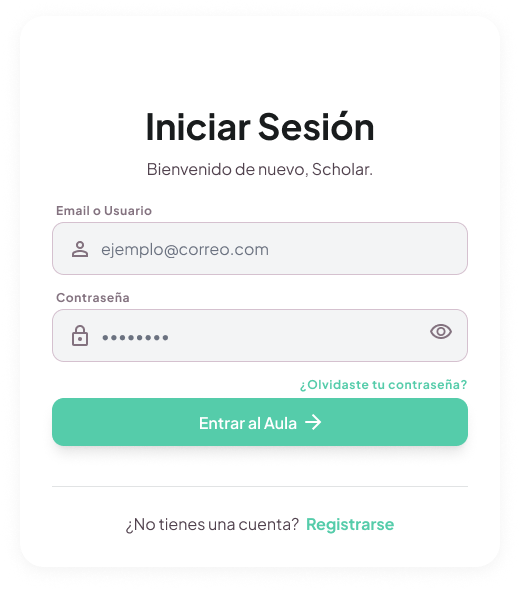
\includegraphics[width=0.45\textwidth]{mockups/01_01_iniciar_sesion.png}
    \caption[Prototipo de inicio de sesión.]{Iniciar sesión.}
    \label{fig:mockup_iniciar_sesion}
\end{figure}

\begin{figure}[H]
    \centering
    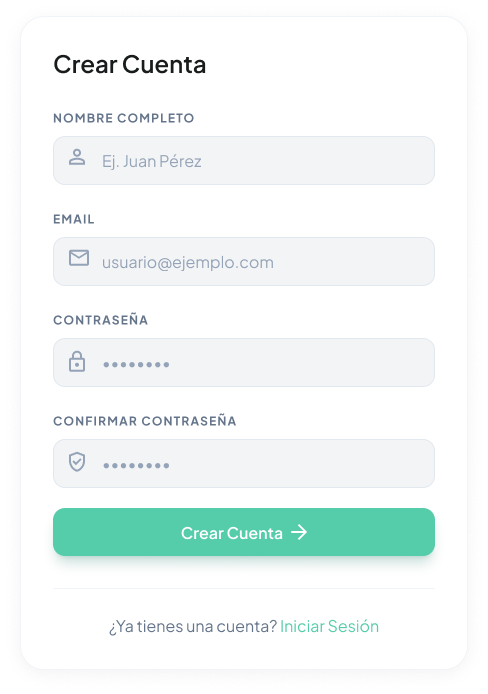
\includegraphics[width=0.5\textwidth]{mockups/01_02_crear_cuenta.png}
    \caption[Prototipo de creación de cuenta.]{Crear cuenta.}
    \label{fig:mockup_crear_cuenta}
\end{figure}

\begin{figure}[H]
    \centering
    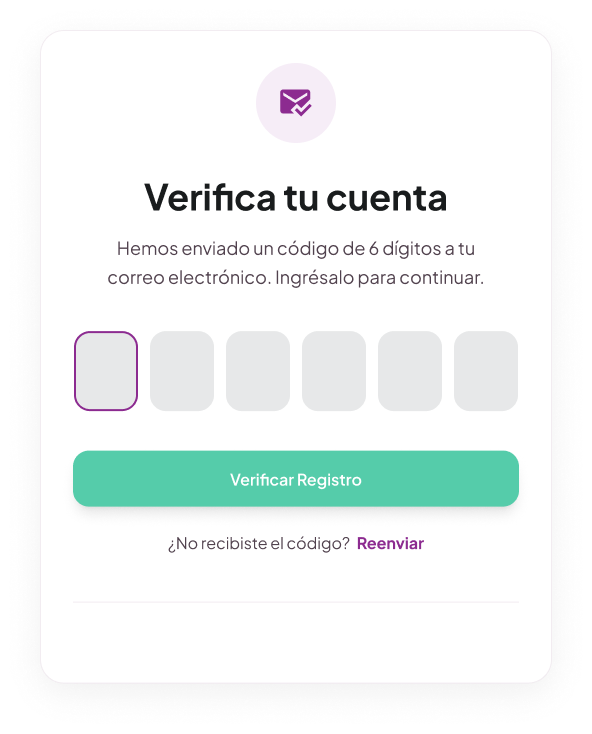
\includegraphics[width=0.53\textwidth]{mockups/01_03_verificar_cuenta.png}
    \caption[Prototipo de verificación de cuenta.]{Verificar cuenta.}
    \label{fig:mockup_verificar_cuenta}
\end{figure}

\section*{Flujo de creación de cuestionarios y gestión de salas}
\label{anexo:flujo_creacion_cuestionarios_gestion_salas}

Comprende el conjunto de interfaces utilizadas por profesor para la preparación de las clases. Incluye creación de cuestionarios (preguntas, opciones y tiempos límite), la consulta del catálogo de cuestionarios creados, la pantalla de configuración de parámetros de la sala y el estado inicial de la sala (en espera).

\begin{figure}[H]
    \centering
    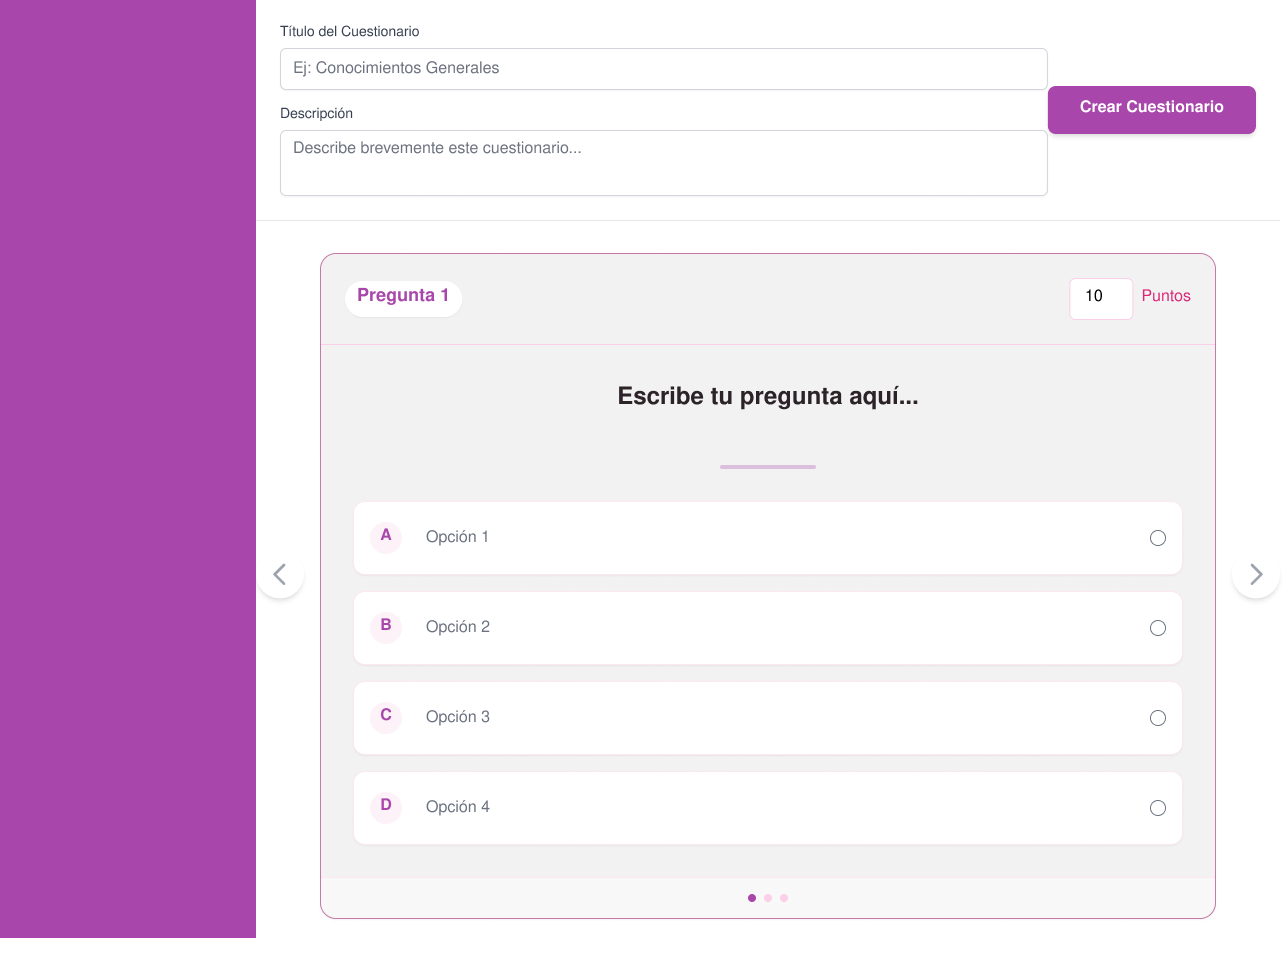
\includegraphics[width=0.75\textwidth]{mockups/02_01_crear_cuestionario.png}
    \caption[Prototipo de creación de cuestionario.]{Crear cuestionario.}
    \label{fig:mockup_crear_cuestionario}
\end{figure}

\begin{figure}[H]
    \centering
    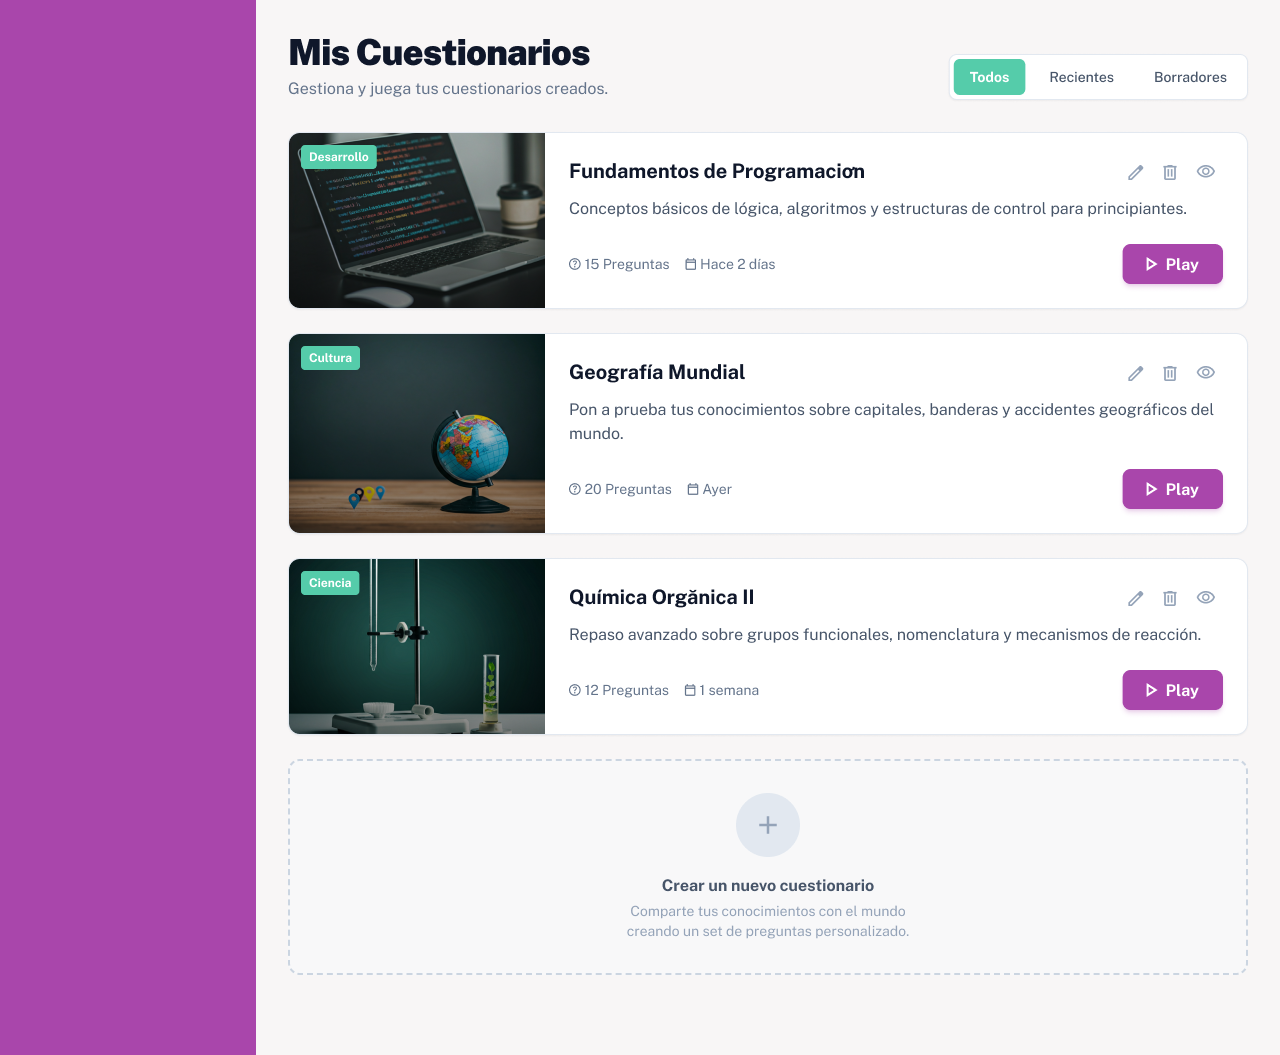
\includegraphics[width=0.7\textwidth]{mockups/02_02_listado_cuestionarios.png}
    \caption[Prototipo de listado de cuestionarios.]{Listado de cuestionarios.}
    \label{fig:mockup_listado_cuestionarios}
\end{figure}

\begin{figure}[H]
    \centering
    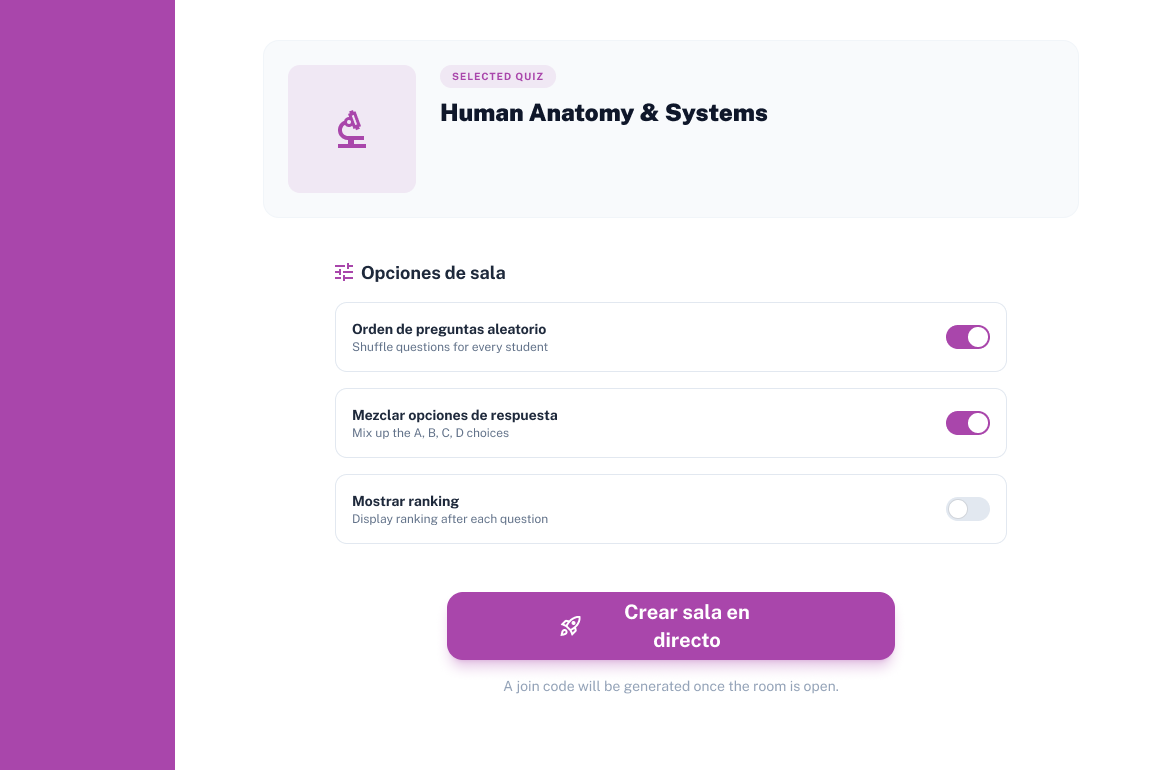
\includegraphics[width=1\textwidth]{mockups/02_03_configuracion_sala.png}
    \caption[Prototipo de configuración de la sala.]{Configuración de la sala.}
    \label{fig:mockup_configuracion_sala}
\end{figure}

\begin{figure}[H]
    \centering
    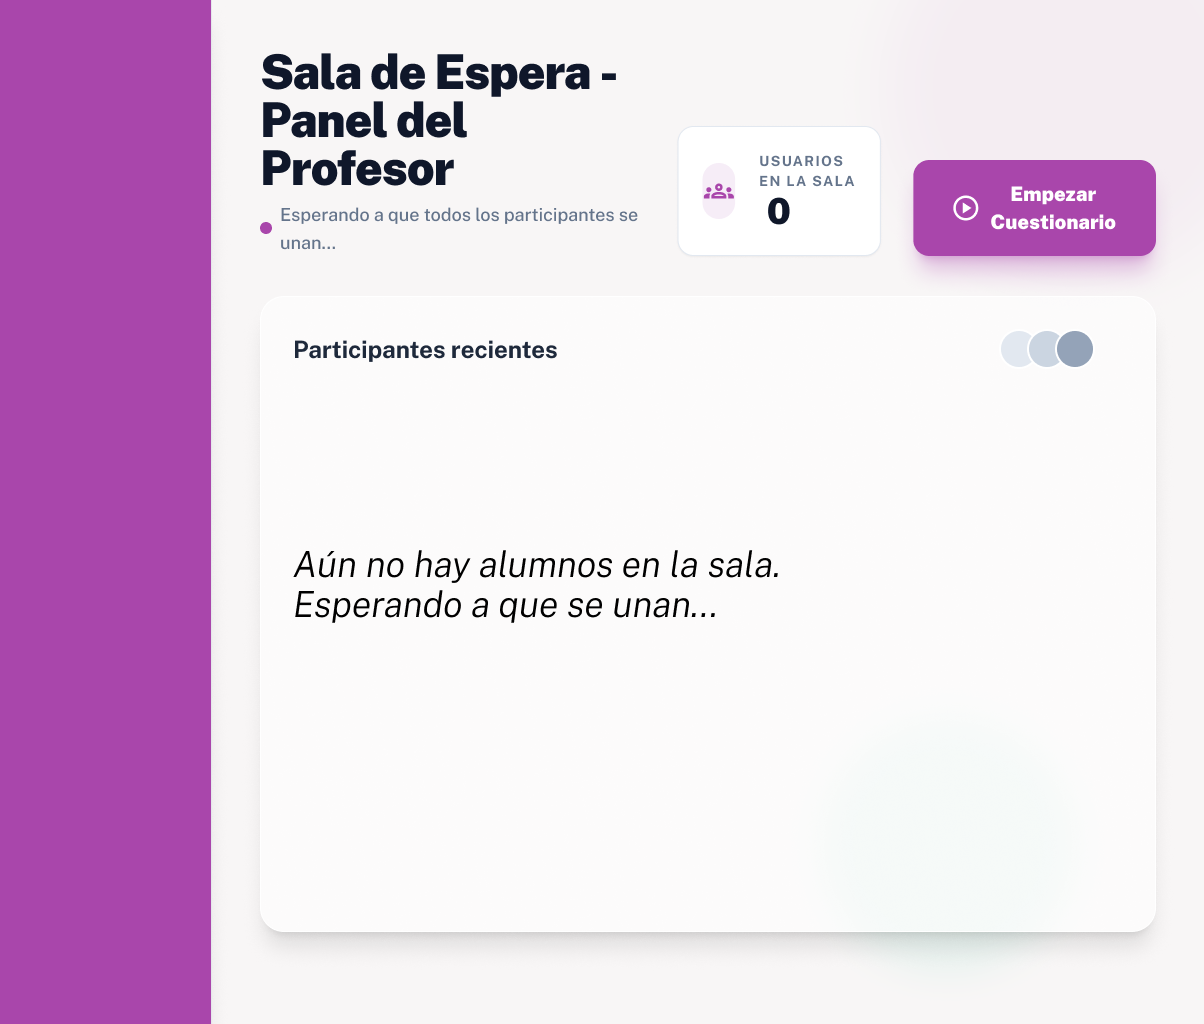
\includegraphics[width=0.8\textwidth]{mockups/02_04_lobby_vacio.png}
    \caption[Prototipo de sala de espera recién creada.]{Sala de espera de la sala recién creada.}
    \label{fig:mockup_lobby_vacio}
\end{figure}

\clearpage

\section*{Flujo de incorporación del estudiante a la sala}
\label{anexo:flujo_incorporacion_estudiante_sala}

Muestra la secuencia que debe seguir un alumno para unirse a una sesión. Inicia con la introducción del código de sala, y continúa con la asignación de su identificador (UVUS o nickname), con su posterior aviso en caso de que el identificador no esté registrado. Por último, muestra la sala de espera hasta el inicio de la partida.

\begin{figure}[H]
    \centering
    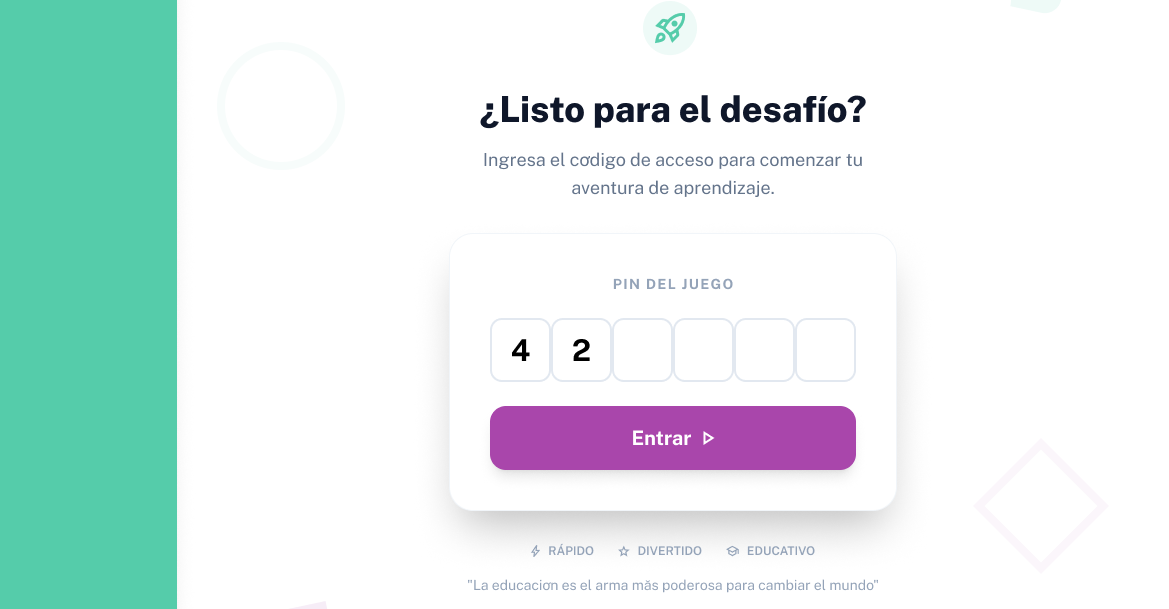
\includegraphics[width=0.95\textwidth]{mockups/03_01_ingresar_codigo.png}
    \caption[Prototipo de \textit{input} de código de sala.]{Ingresar código de sala.}
    \label{fig:mockup_ingresar_codigo}
\end{figure}

\begin{figure}[H]
    \centering
    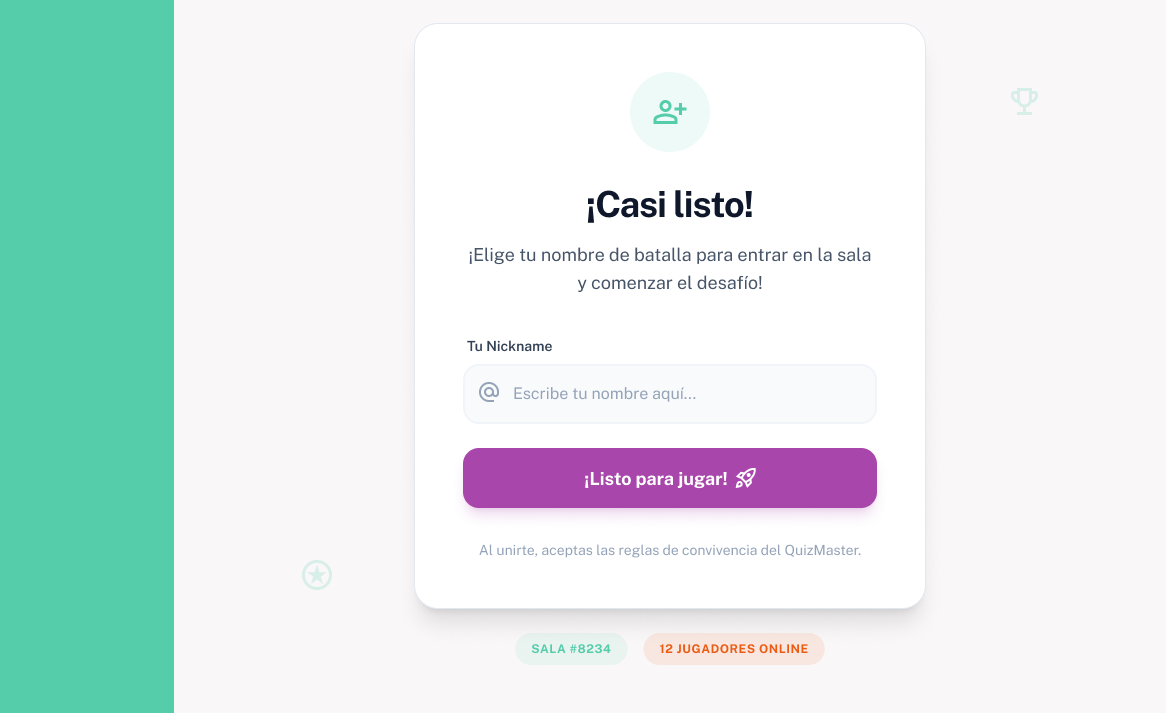
\includegraphics[width=0.95\textwidth]{mockups/03_02_ingresar_nickname.png}
    \caption[Prototipo de \textit{input} de UVUS o nickname.]{Ingresar UVUS o nickname.}
    \label{fig:mockup_ingresar_nickname}
\end{figure}

\begin{figure}[H]
    \centering
    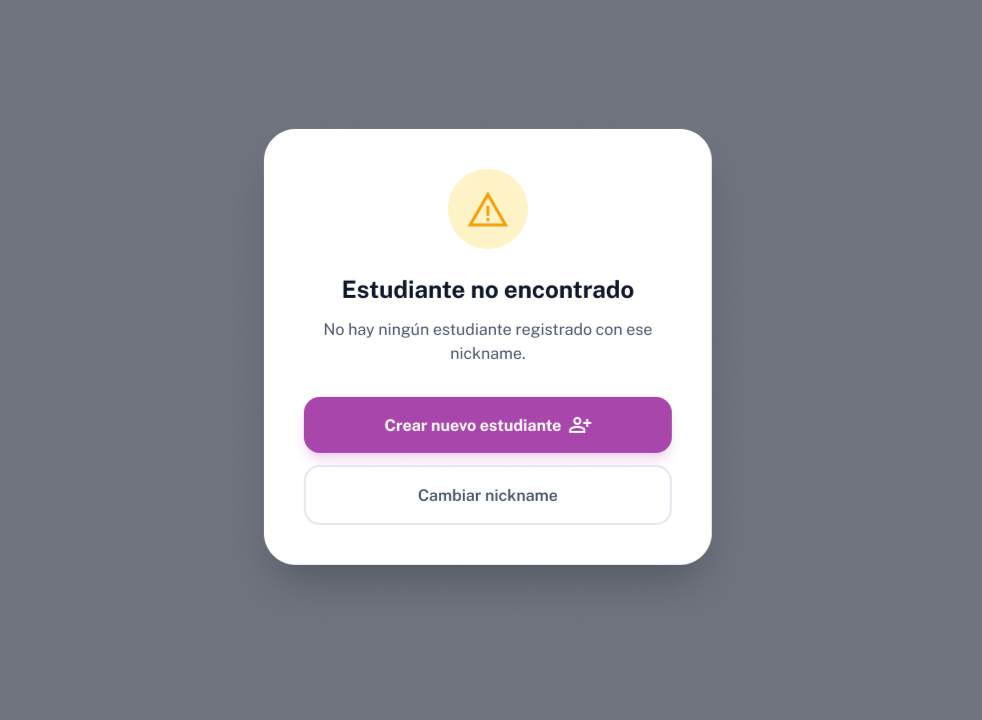
\includegraphics[width=0.9\textwidth]{mockups/03_03_nuevo_nickname.png}
    \caption[Prototipo de aviso para registrar nuevo UVUS o nickname.]{Aviso para registrar nuevo UVUS o nickname.}
    \label{fig:mockup_nuevo_nickname}
\end{figure}

\begin{figure}[H]
    \centering
    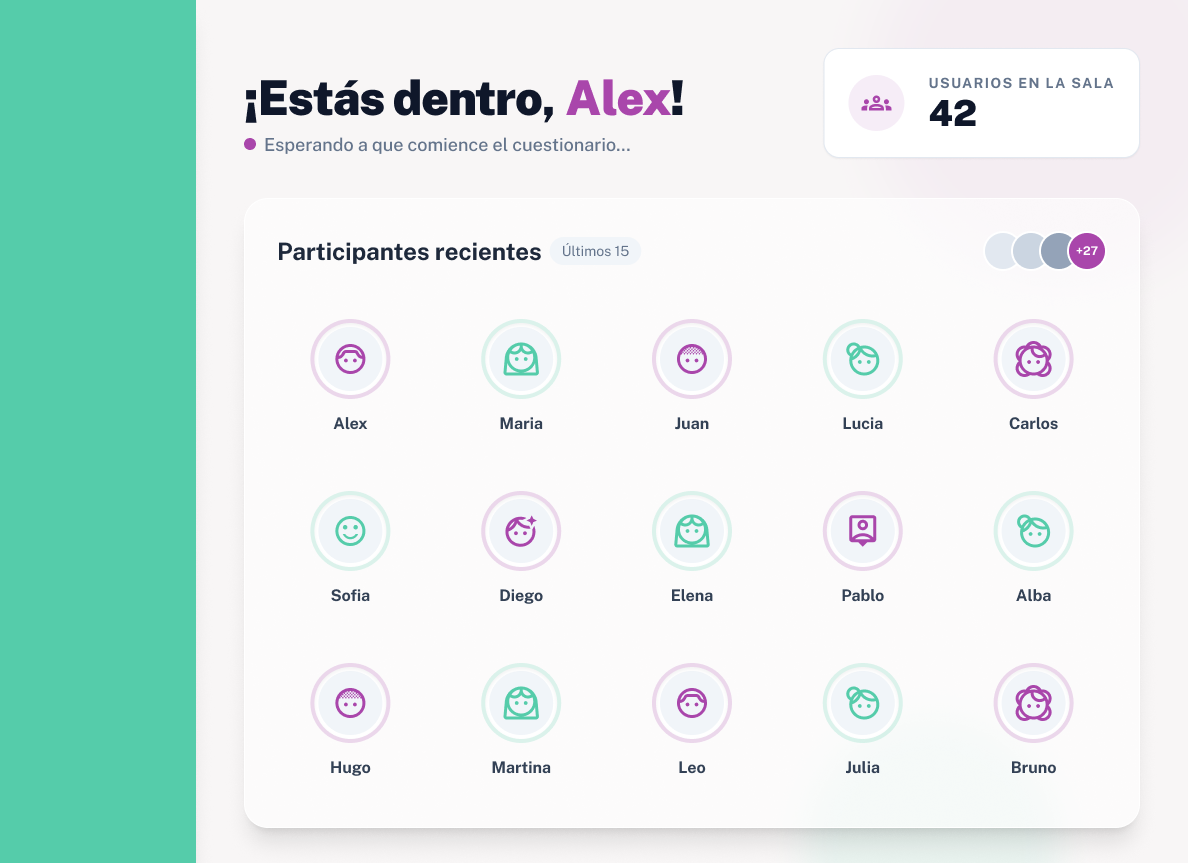
\includegraphics[width=1\textwidth]{mockups/03_04_lobby_alumno.png}
    \caption[Prototipo de sala de espera del alumno recién ingresado.]{Sala de espera del alumno recién ingresado.}
    \label{fig:mockup_lobby_alumno}
\end{figure}

\clearpage

\section*{Flujo de ejecución de la partida en vivo}
\label{anexo:flujo_ejecucion_partida_vivo}

Describe la interacción en tiempo real durante el desarrollo de una sala. Para comparar la experiencia del profesor y del alumno, se presentan en paralelo las interfaces que muestran divergencias funcionales o de diseño. El flujo abarca las fases de sala de espera activa, lectura de pregunta, envío de respuestas, retroalimentación inmediata, tabla de clasificación y verificación final.

\begin{figure}[H]
    \centering
    \makebox[\textwidth][c]{%
        \begin{minipage}{0.57\textwidth}
            \centering
            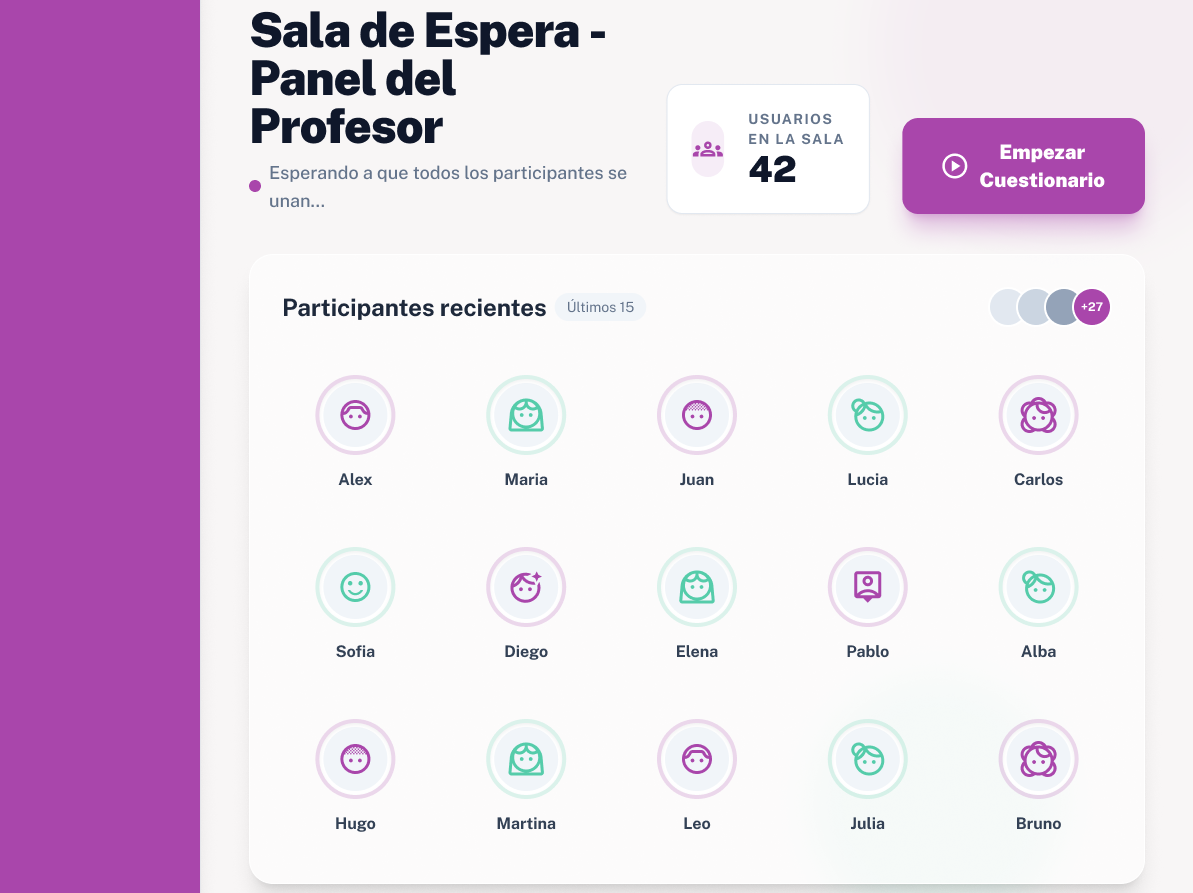
\includegraphics[width=\textwidth]{mockups/04_01_lobby_profesor.png}
            \caption*{Vista Profesor}
        \end{minipage}%
        \hfill
        \begin{minipage}{0.57\textwidth}
            \centering
            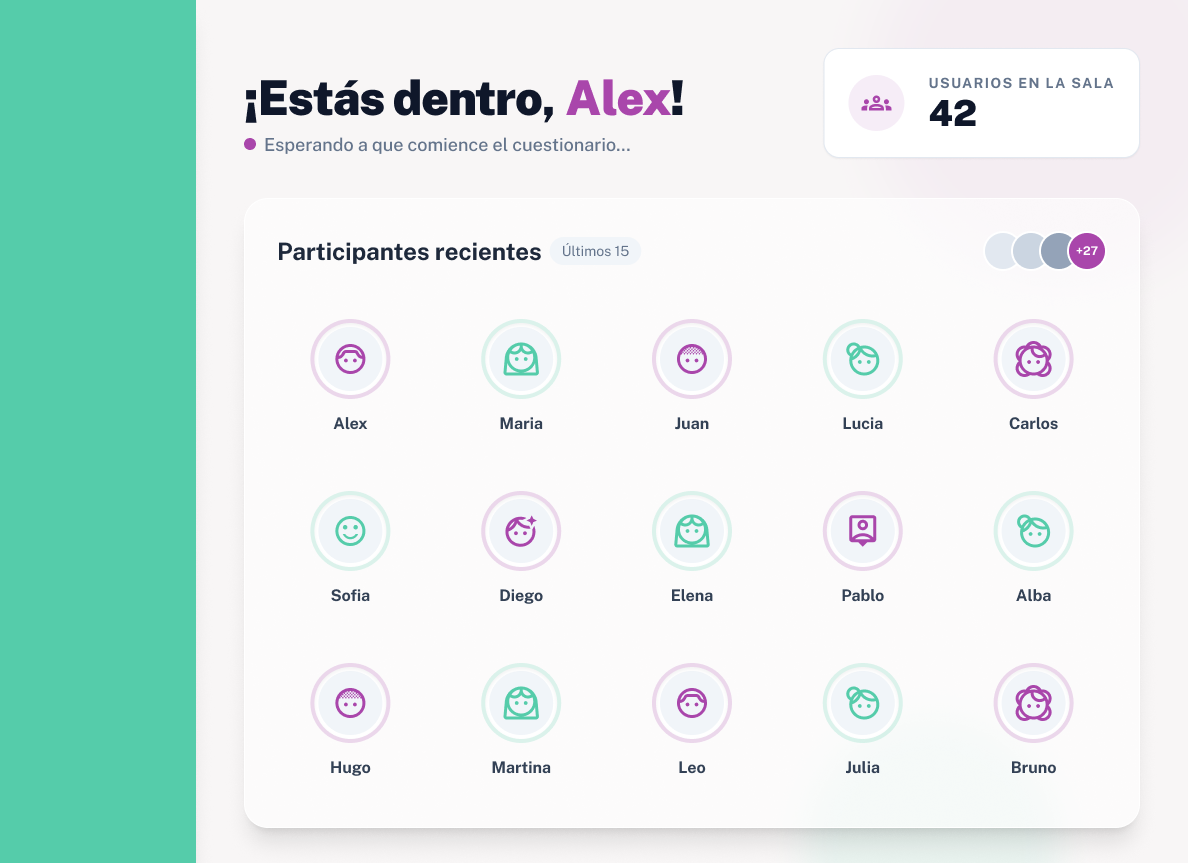
\includegraphics[width=\textwidth]{mockups/04_01_lobby_alumno.png}
            \caption*{Vista Alumno}
        \end{minipage}%
    }
    \caption[Prototipo de sala de espera.]{Sala de espera.}
    \label{fig:mockup_lobby}
\end{figure}

\begin{figure}[H]
    \centering
    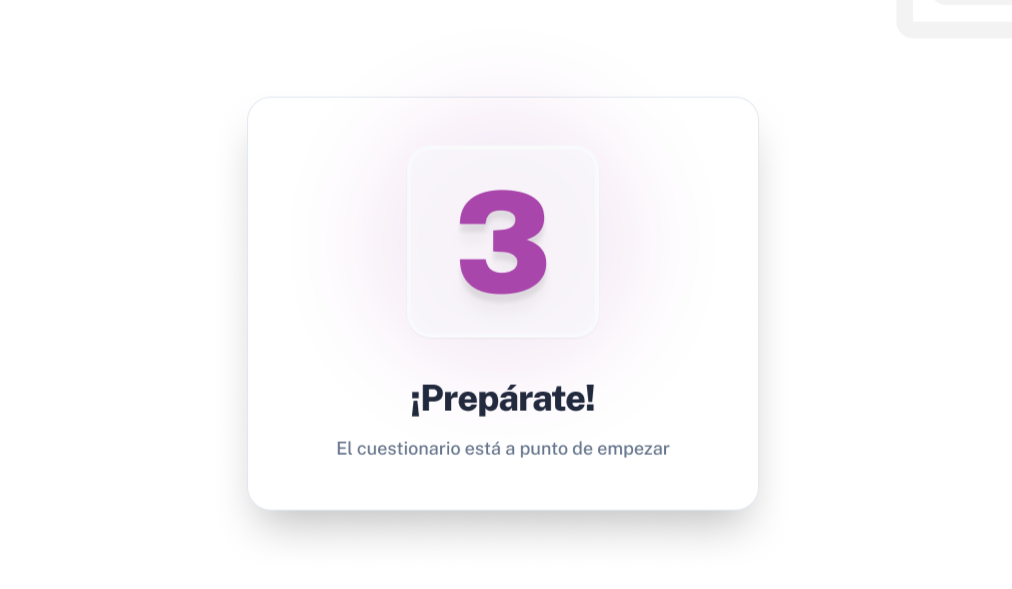
\includegraphics[width=1\textwidth]{mockups/04_02_cuenta_atras.png}
    \caption[Prototipo de cuenta atrás.]{Cuenta atrás.}
    \label{fig:mockup_cuenta_atras}
\end{figure}

\begin{figure}[H]
    \centering
    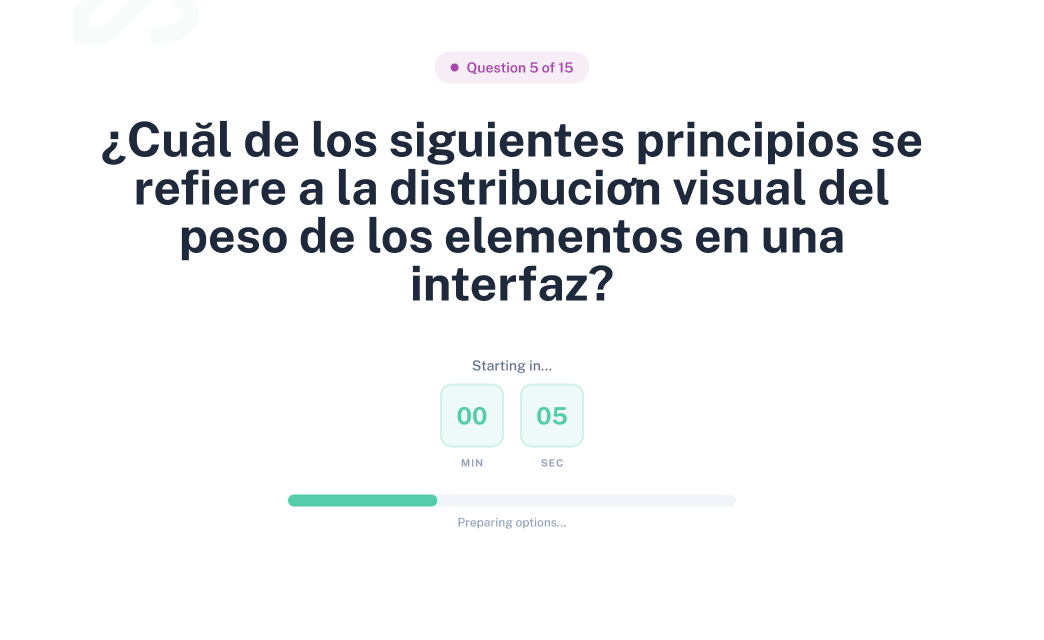
\includegraphics[width=1\textwidth]{mockups/04_03_leer_pregunta.png}
    \caption[Prototipo de tiempo de lectura de pregunta.]{Tiempo de lectura de pregunta.}
    \label{fig:mockup_leer_pregunta}
\end{figure}

\begin{figure}[H]
    \centering
    \makebox[\textwidth][c]{%
        \begin{minipage}{0.57\textwidth}
            \centering
            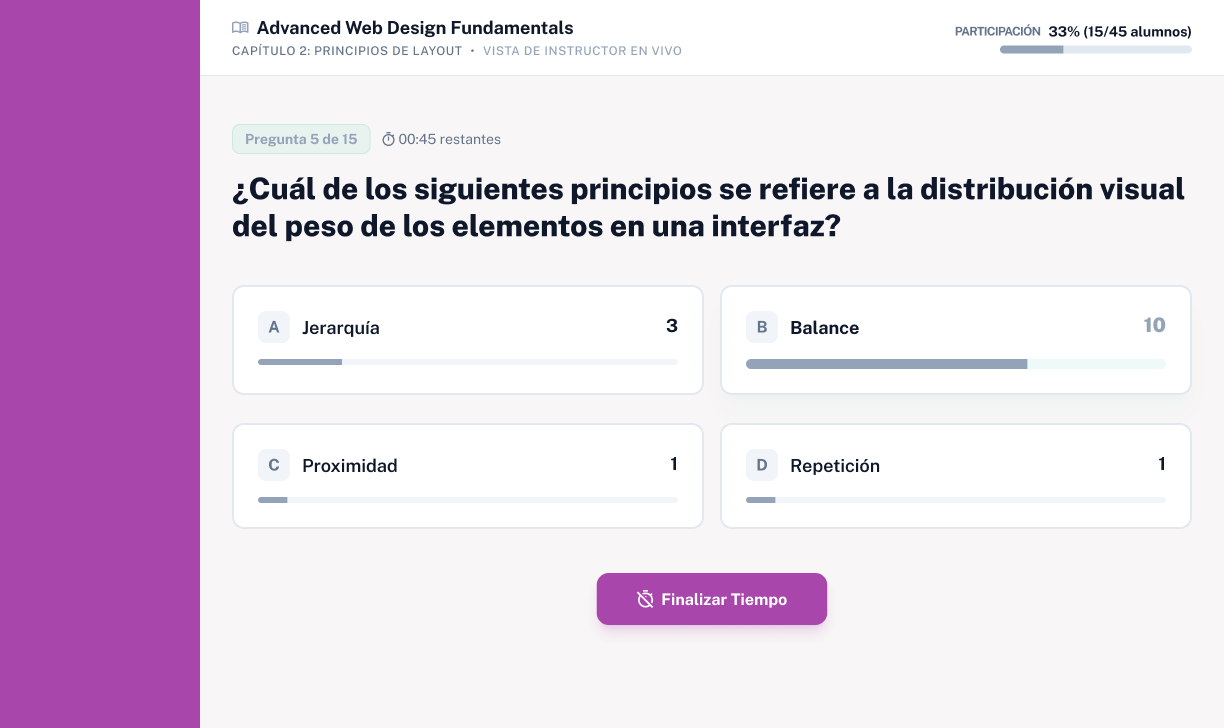
\includegraphics[width=\textwidth]{mockups/04_04_pregunta_profesor.png}
            \caption*{(a) Vista Profesor}
        \end{minipage}%
        \hfill
        \begin{minipage}{0.57\textwidth}
            \centering
            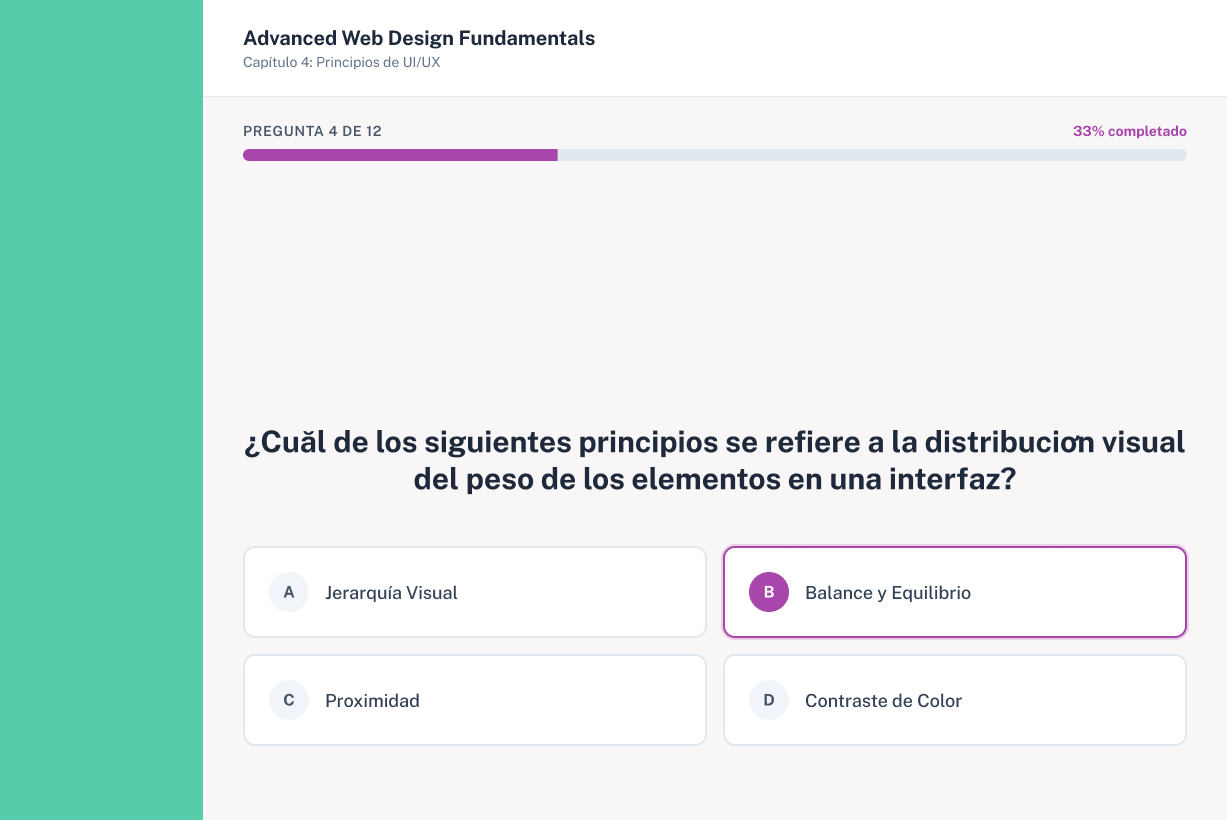
\includegraphics[width=\textwidth]{mockups/04_04_pregunta_alumno.png}
            \caption*{(b) Vista Alumno}
        \end{minipage}%
    }
    \caption[Prototipo de pregunta en curso y envío de respuesta.]{Pregunta en curso y envío de respuesta.}
    \label{fig:mockup_pregunta}
\end{figure}

\begin{figure}[H]
    \centering
    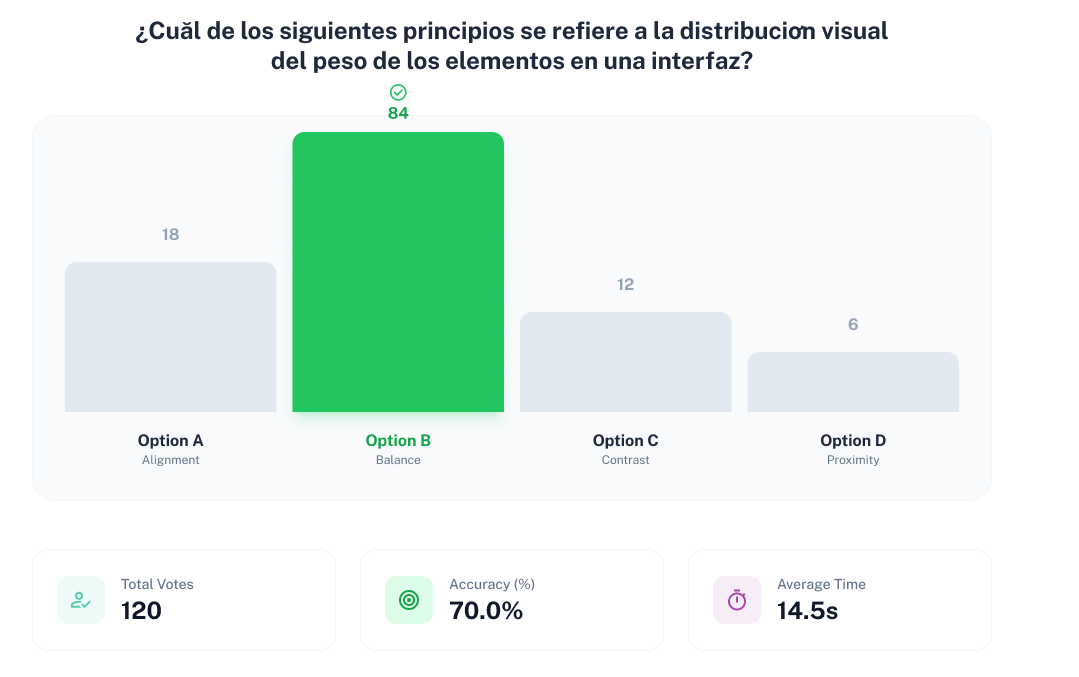
\includegraphics[width=1\textwidth]{mockups/04_05_mostrar_respuesta.png}
    \caption[Prototipo de resultados de la pregunta.]{Resultados de la pregunta.}
    \label{fig:mockup_mostrar_respuesta}
\end{figure}

\begin{figure}[H]
    \centering
    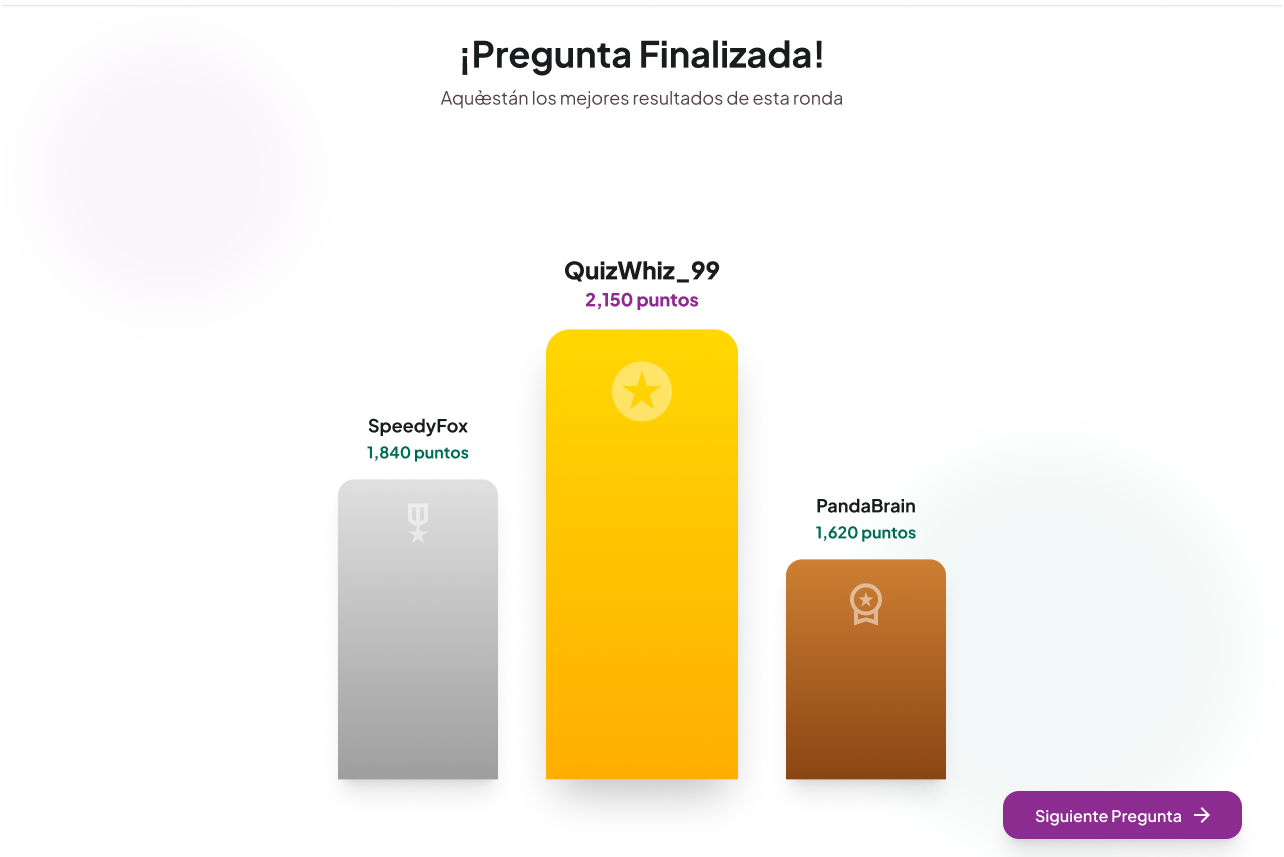
\includegraphics[width=1\textwidth]{mockups/04_06_ranking.png}
    \caption[Prototipo de podio de puntuaciones.]{Podio de puntuaciones.}
    \label{fig:mockup_ranking}
\end{figure}

\begin{figure}[H]
    \centering
    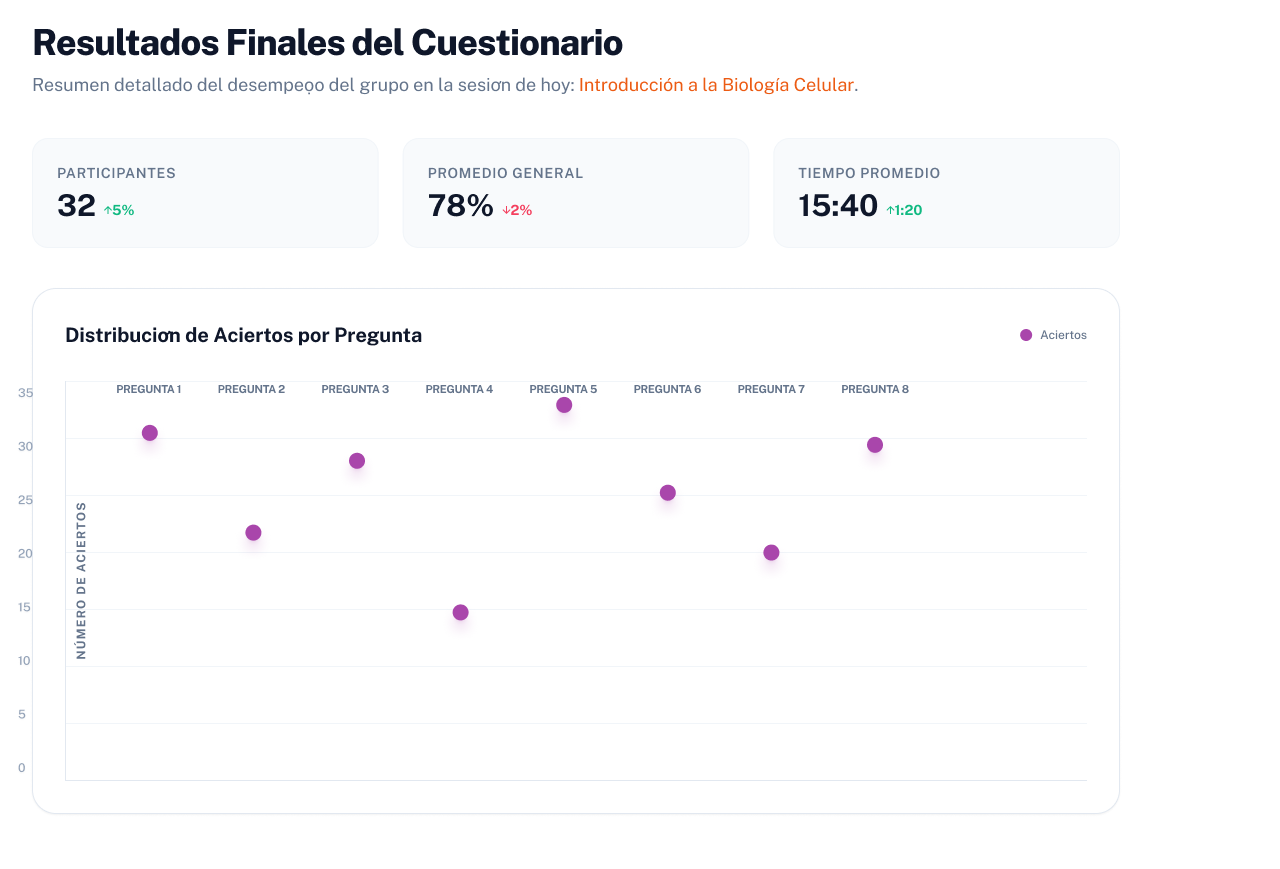
\includegraphics[width=1\textwidth]{mockups/04_07_distribucion_respuestas.png}
    \caption[Prototipo de visualización global de respuestas.]{Distribución global de respuestas.}
    \label{fig:mockup_distribucion_respuestas}
\end{figure}

\begin{figure}[H]
    \centering
    \makebox[\textwidth][c]{%
        \begin{minipage}{0.57\textwidth}
            \centering
            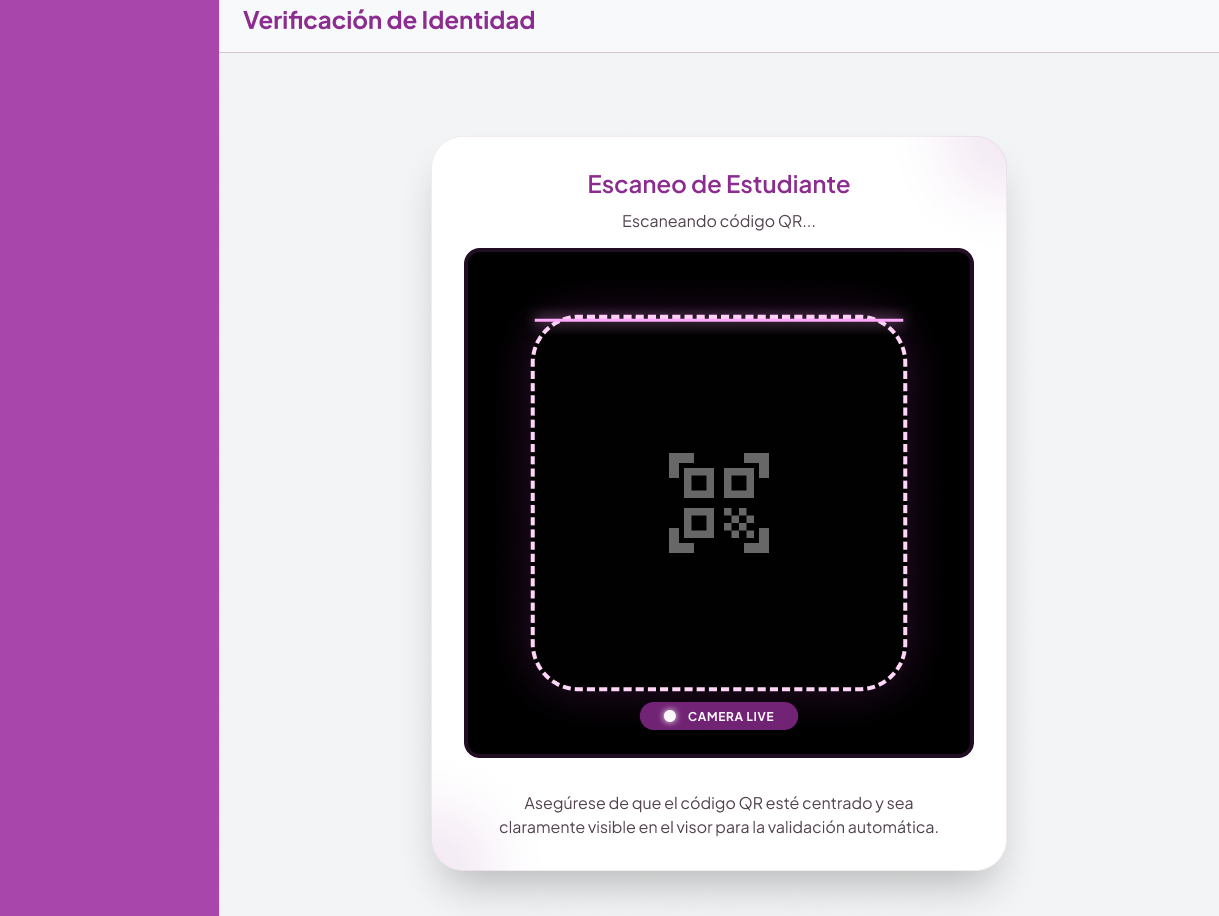
\includegraphics[width=\textwidth]{mockups/04_08_verificacion_profesor.png}
            \caption*{(a) Vista Profesor}
        \end{minipage}%
        \hfill
        \begin{minipage}{0.57\textwidth}
            \centering
            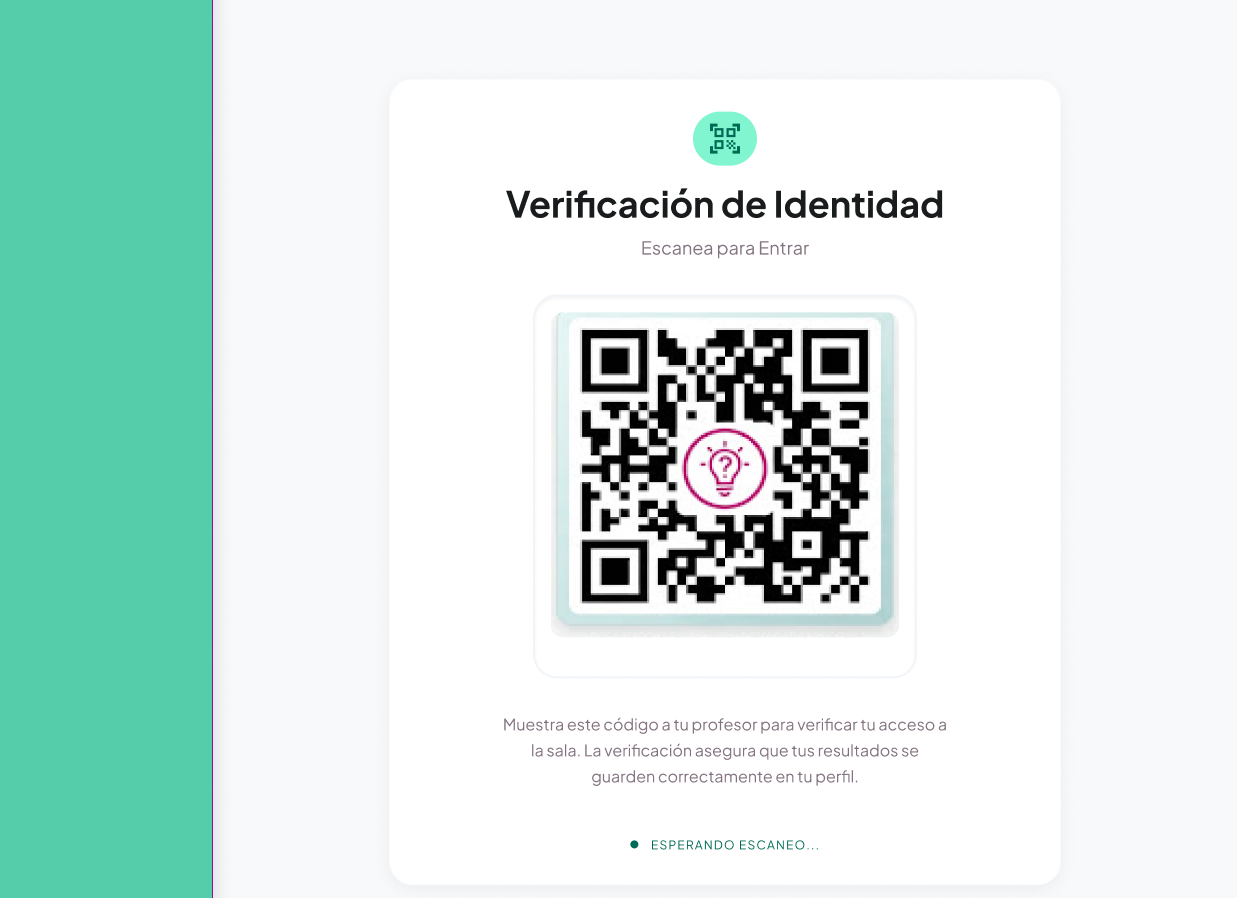
\includegraphics[width=\textwidth]{mockups/04_08_verificacion_alumno.png}
            \caption*{(b) Vista Alumno}
        \end{minipage}%
    }
    \caption[Prototipo de verificación final.]{Verificación final.}
    \label{fig:mockup_verificacion}
\end{figure}

\end{appendices}
    \begin{appendices}
\chapter{Manual de usuario}\label{anexo:manual_de_usuario}

El presente manual de usuario tiene como objetivo proporcionar una guía detallada y visual para la utilización de la plataforma \textit{Quizzie}. A diferencia de un catálogo estático de pantallas, este documento estructura la guía siguiendo la experiencia de usuario cronológica real: desde el punto de entrada a la aplicación web y el acceso diferenciado por roles, hasta la navegación por el panel principal, la preparación de contenidos y el desarrollo completo de una sesión interactiva en tiempo real.

\section*{Punto de entrada a la aplicación y roles de usuario}

Al navegar a la dirección raíz del sitio web (\texttt{/}), la plataforma ofrece una interfaz unificada adaptada a los dos perfiles principales:

\begin{itemize}
    \item[\tiny$\blacksquare$] \textbf{Alumno:} Accede directamente desde la pantalla de bienvenida introduciendo el código PIN proyectado en el aula, sin necesidad de contraseñas ni registros previos.
    \item[\tiny$\blacksquare$] \textbf{Profesor:} Dispone de accesos dedicados para iniciar sesión (\texttt{/login}) o registrarse (\texttt{/register}). Tras autenticarse, accede a un panel de control privado con una barra de navegación lateral (\textit{sidebar}) para gestionar sus cuestionarios y salas.
\end{itemize}

\section*{Registro, autenticación y gestión del perfil docente}

El ciclo de vida del usuario docente comienza desde la pantalla principal de la plataforma, guiando al profesor a través de un proceso de registro con correo electrónico, la administración de su cuenta y los mecanismos de recuperación de acceso.

\subsection*{1. Acceso inicial a la plataforma}

Al acceder a la aplicación web, el profesor visualiza la pantalla de inicio, la cual permite iniciar sesión o registrarse, o bien saltar a la zona de estudiantes.

\begin{figure}[H]
  \centering
  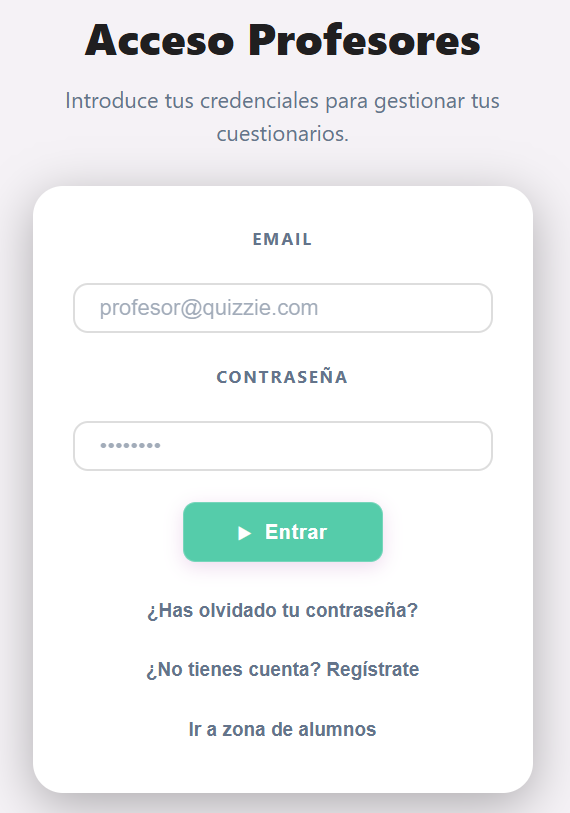
\includegraphics[width=0.42\textwidth]{screenshots/inicio.png}
  \caption{Punto de entrada a la plataforma.}
  \label{fig:manual_inicio}
\end{figure}

\subsection*{2. Formulario de registro docente}

Al pulsar sobre la opción de registro, el sistema presenta un formulario donde el profesor debe ingresar su nombre, dirección de correo electrónico y una contraseña.

\begin{figure}[H]
  \centering
  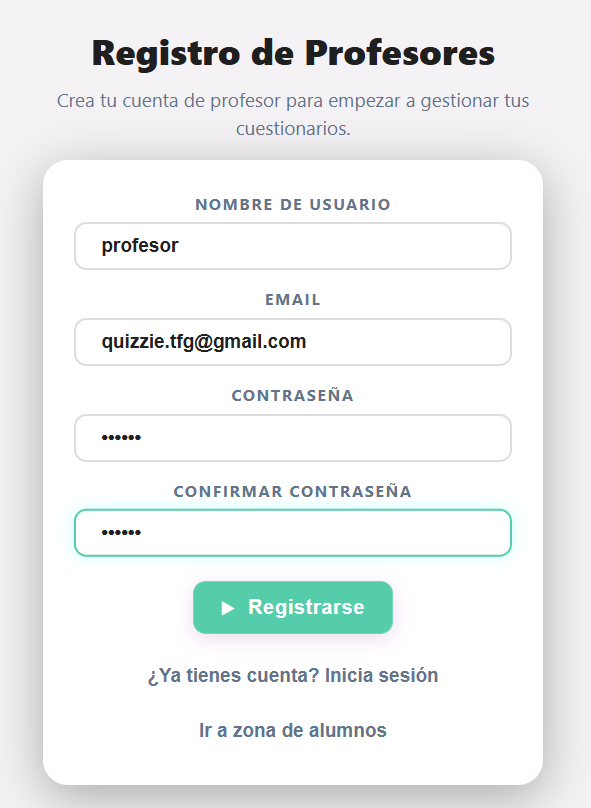
\includegraphics[width=0.44\textwidth]{screenshots/registro.png}
  \caption{Formulario de registro para el perfil docente.}
  \label{fig:manual_registro}
\end{figure}

\subsection*{3. Notificación de verificación de cuenta}

Una vez completado y enviado el formulario, la plataforma envía un correo electrónico a la dirección facilitada con un código numérico temporal de un solo uso para verificar la cuenta.

\begin{figure}[H]
  \centering
  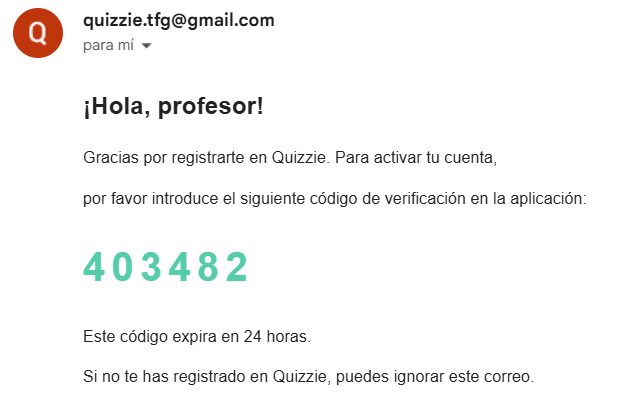
\includegraphics[width=0.6\textwidth]{screenshots/correo_verificar_cuenta.png}
  \caption{Correo electrónico con el código de verificación de cuenta.}
  \label{fig:manual_correo_verificar}
\end{figure}

\subsection*{4. Confirmación del código y activación}

El profesor es redirigido a una vista específica donde debe introducir el código recibido en el correo. Al pulsar sobre el botón de confirmación, la cuenta queda validada en la base de datos y habilitada para su uso.

\begin{figure}[H]
  \centering
  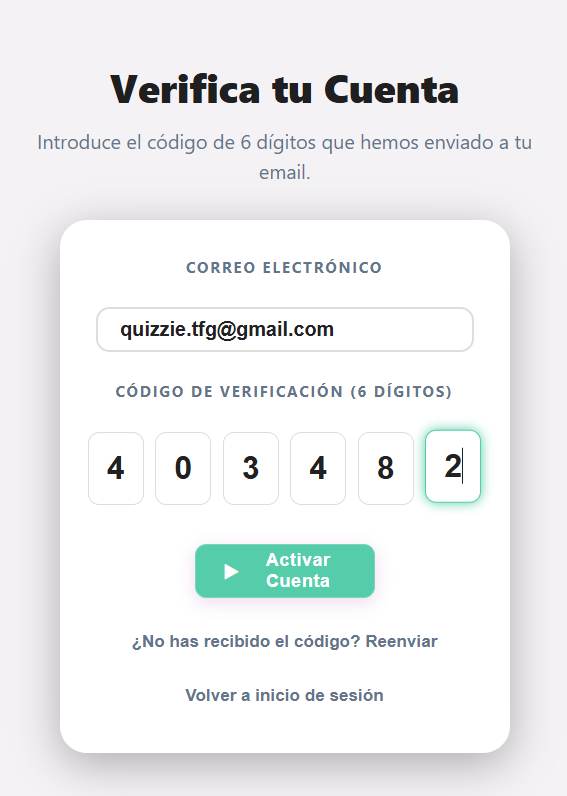
\includegraphics[width=0.42\textwidth]{screenshots/verificar_cuenta.png}
  \caption{Pantalla de introducción del código de verificación de cuenta.}
  \label{fig:manual_verificar_cuenta}
\end{figure}

\subsection*{5. Panel y opciones del perfil}

Tras iniciar sesión, el docente puede acceder a la sección de su perfil personal. Desde esta vista se muestran los datos del usuario y se facilitan las acciones de actualización de datos, cambio de contraseña o borrado de la cuenta.

\begin{figure}[H]
  \centering
  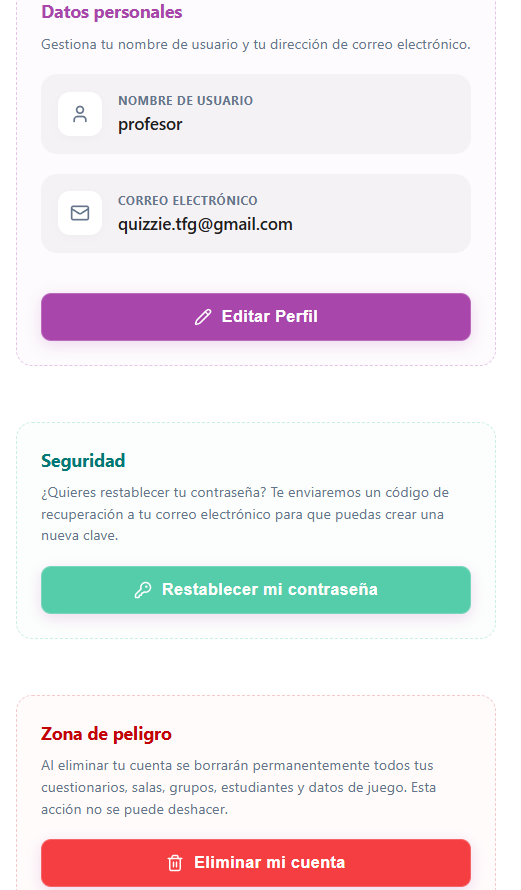
\includegraphics[width=0.6\textwidth]{screenshots/mi_perfil.png}
  \caption{Vista de gestión del perfil docente.}
  \label{fig:manual_mi_perfil}
\end{figure}

\subsection*{6. Solicitud y correo de restablecimiento de contraseña}

Si el profesor solicita una modificación o recuperación de contraseña, el sistema envía un nuevo correo electrónico que contiene el código de autorización requerido para efectuar dicho cambio.

\begin{figure}[H]
  \centering
  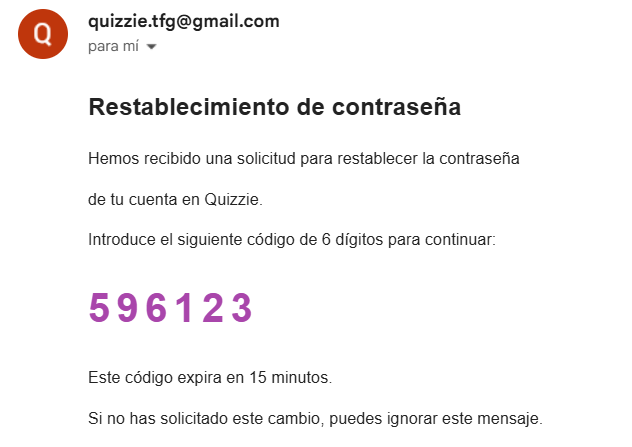
\includegraphics[width=0.62\textwidth]{screenshots/correo_cambiar_contra.png}
  \caption{Correo electrónico para el restablecimiento de contraseña.}
  \label{fig:manual_correo_cambiar_contra}
\end{figure}

\subsection*{7. Introducción de nueva contraseña}

En la interfaz, el usuario introduce el código de un solo uso recibido por correo junto con su nueva clave de acceso, efectuándose así la actualización de la contraseña.

\begin{figure}[H]
  \centering
  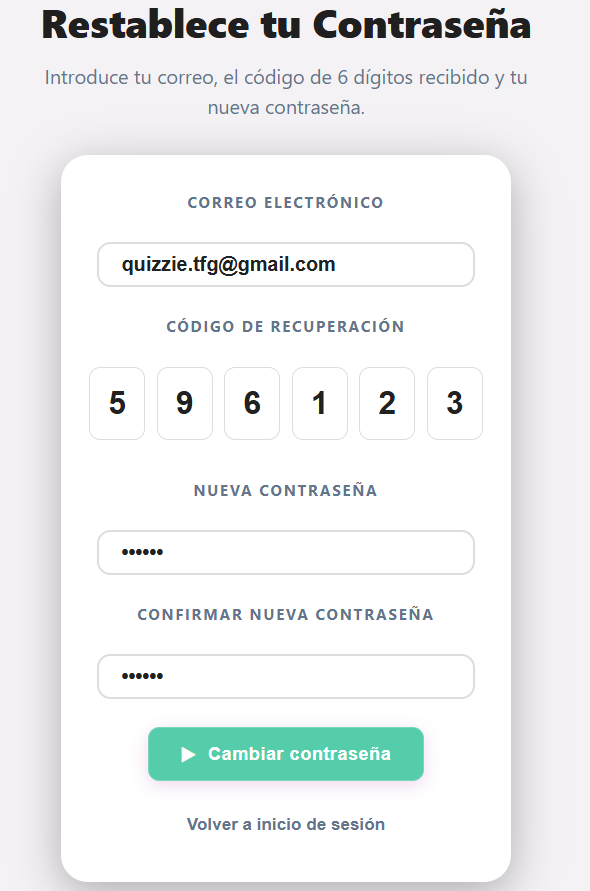
\includegraphics[width=0.45\textwidth]{screenshots/restablecer_contra.png}
  \caption{Formulario para establecer la nueva contraseña.}
  \label{fig:manual_restablecer_contra}
\end{figure}

\subsection*{8. Eliminación definitiva de la cuenta}

Finalmente, la plataforma contempla el derecho al borrado de datos. El docente puede solicitar la supresión completa de su perfil y datos asociados mediante un diálogo de confirmación que advierte sobre la irreversibilidad de la acción.

\begin{figure}[H]
  \centering
  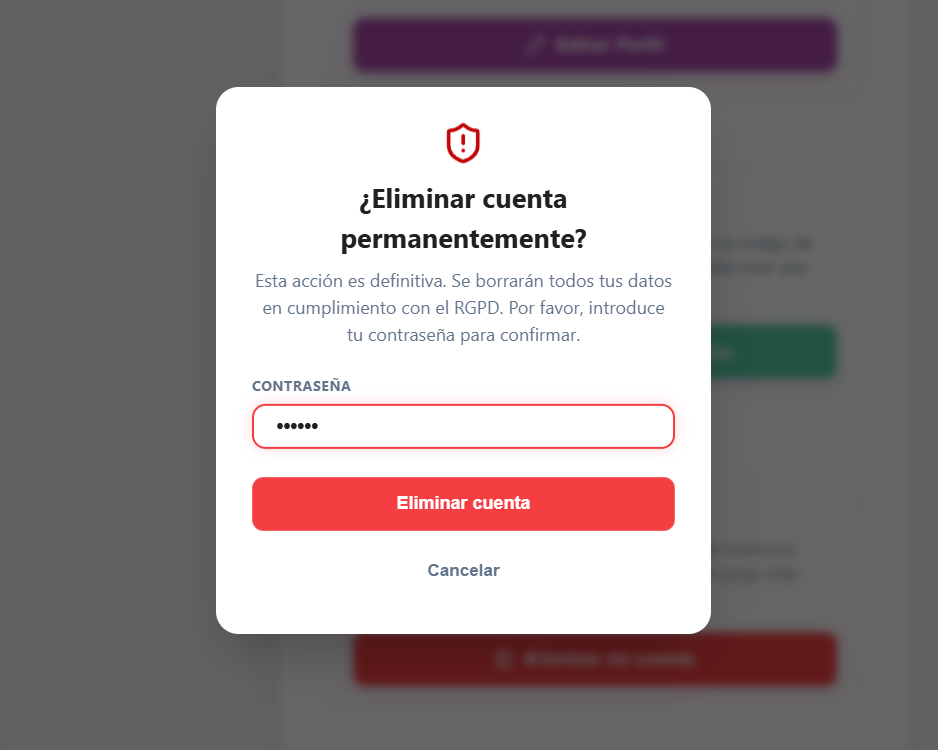
\includegraphics[width=0.85\textwidth]{screenshots/eliminar_cuenta.png}
  \caption{Confirmación de eliminación de la cuenta de usuario.}
  \label{fig:manual_eliminar_cuenta}
\end{figure}

\section*{Gestión del catálogo de cuestionarios e historial docente}\label{sec:manual_gestion_cuestionarios}

Una vez autenticado en la plataforma, el docente dispone de un entorno centralizado para la administración de sus contenidos académicos. Desde este espacio es posible consultar el catálogo de pruebas creadas, editar sus preguntas y parámetros, examinar las métricas de sesiones anteriores, exportar los resultados y crear nuevos cuestionarios.

\subsection*{1. Inicio de sesión del profesor}

El docente introduce su correo electrónico y contraseña en el formulario de acceso para ingresar a su panel privado de control.

\begin{figure}[H]
  \centering
  \makebox[\textwidth][c]{%
    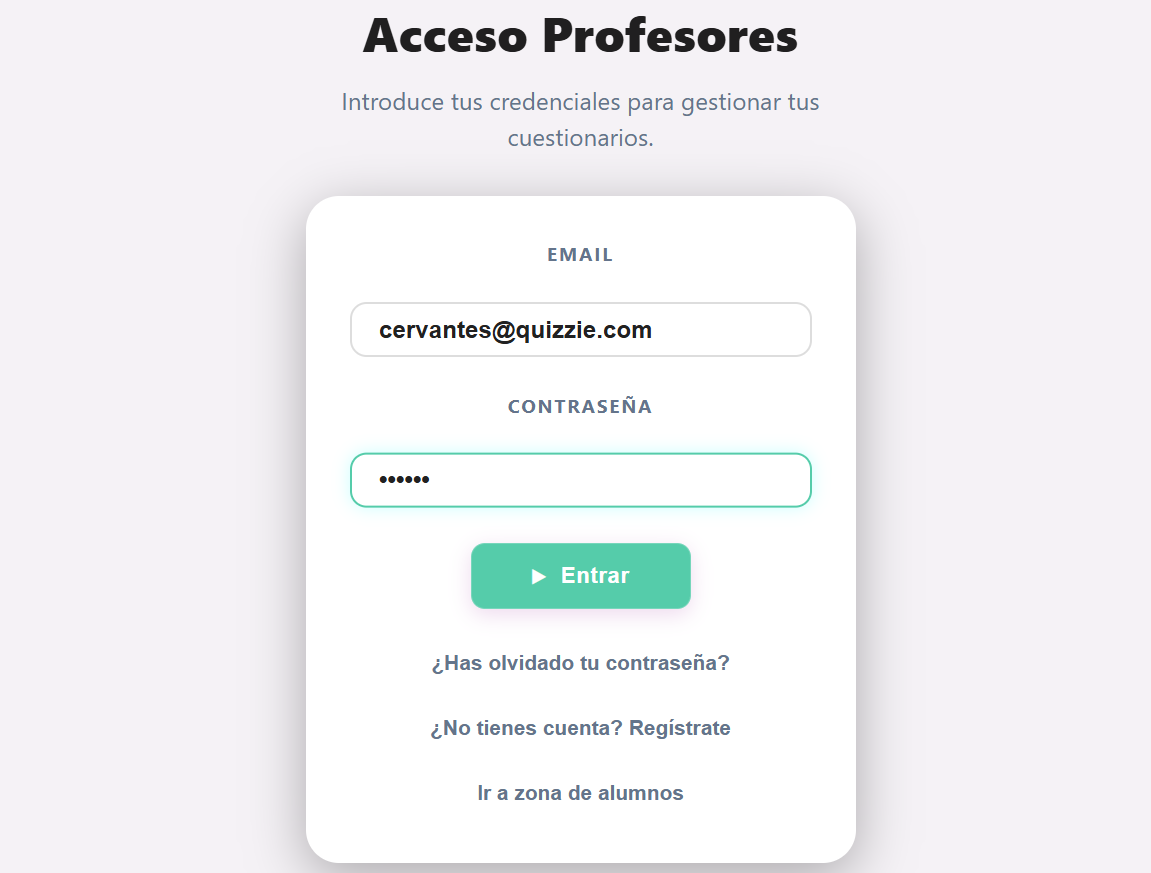
\includegraphics[width=0.8\textwidth]{screenshots/iniciar_sesion.png}%
  }
  \caption{Formulario de inicio de sesión.}
  \label{fig:manual_iniciar_sesion}
\end{figure}

\subsection*{2. Catálogo de cuestionarios disponibles}

Al acceder a la sección de cuestionarios, el profesor visualiza la lista con todas sus pruebas creadas. Cada entrada dispone de tres acciones rápidas: el icono del lápiz para modificar el cuestionario, el ojo para consultar el historial de salas asociadas y la papelera para su eliminación.

\begin{figure}[H]
  \centering
  \makebox[\textwidth][c]{%
    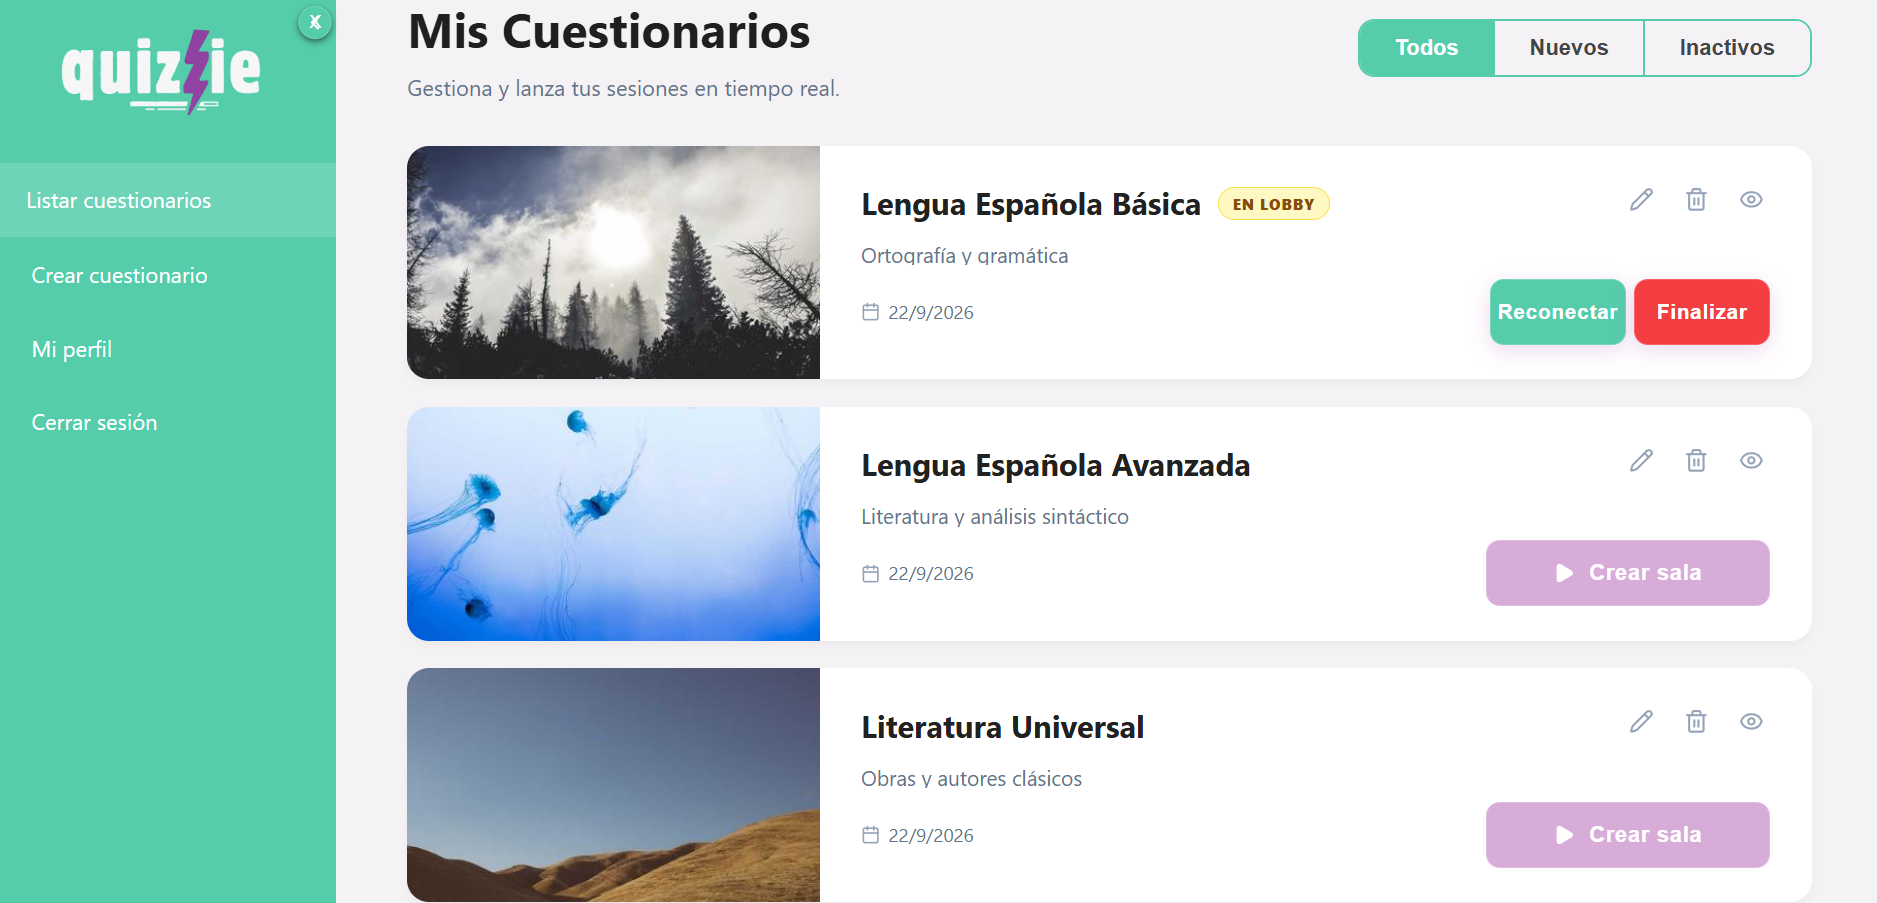
\includegraphics[width=1.1\textwidth]{screenshots/mis_cuestionarios.png}%
  }
  \caption{Listado general de cuestionarios del profesor.}
  \label{fig:manual_mis_cuestionarios}
\end{figure}

\subsection*{3. Edición de cuestionario}

Pulsando sobre el botón de edición, se abre el formulario donde es posible cambiar el título, modificar su descripción o ajustar el contenido, opciones y puntajes de las preguntas existentes.

\begin{figure}[H]
  \centering
  \makebox[\textwidth][c]{%
    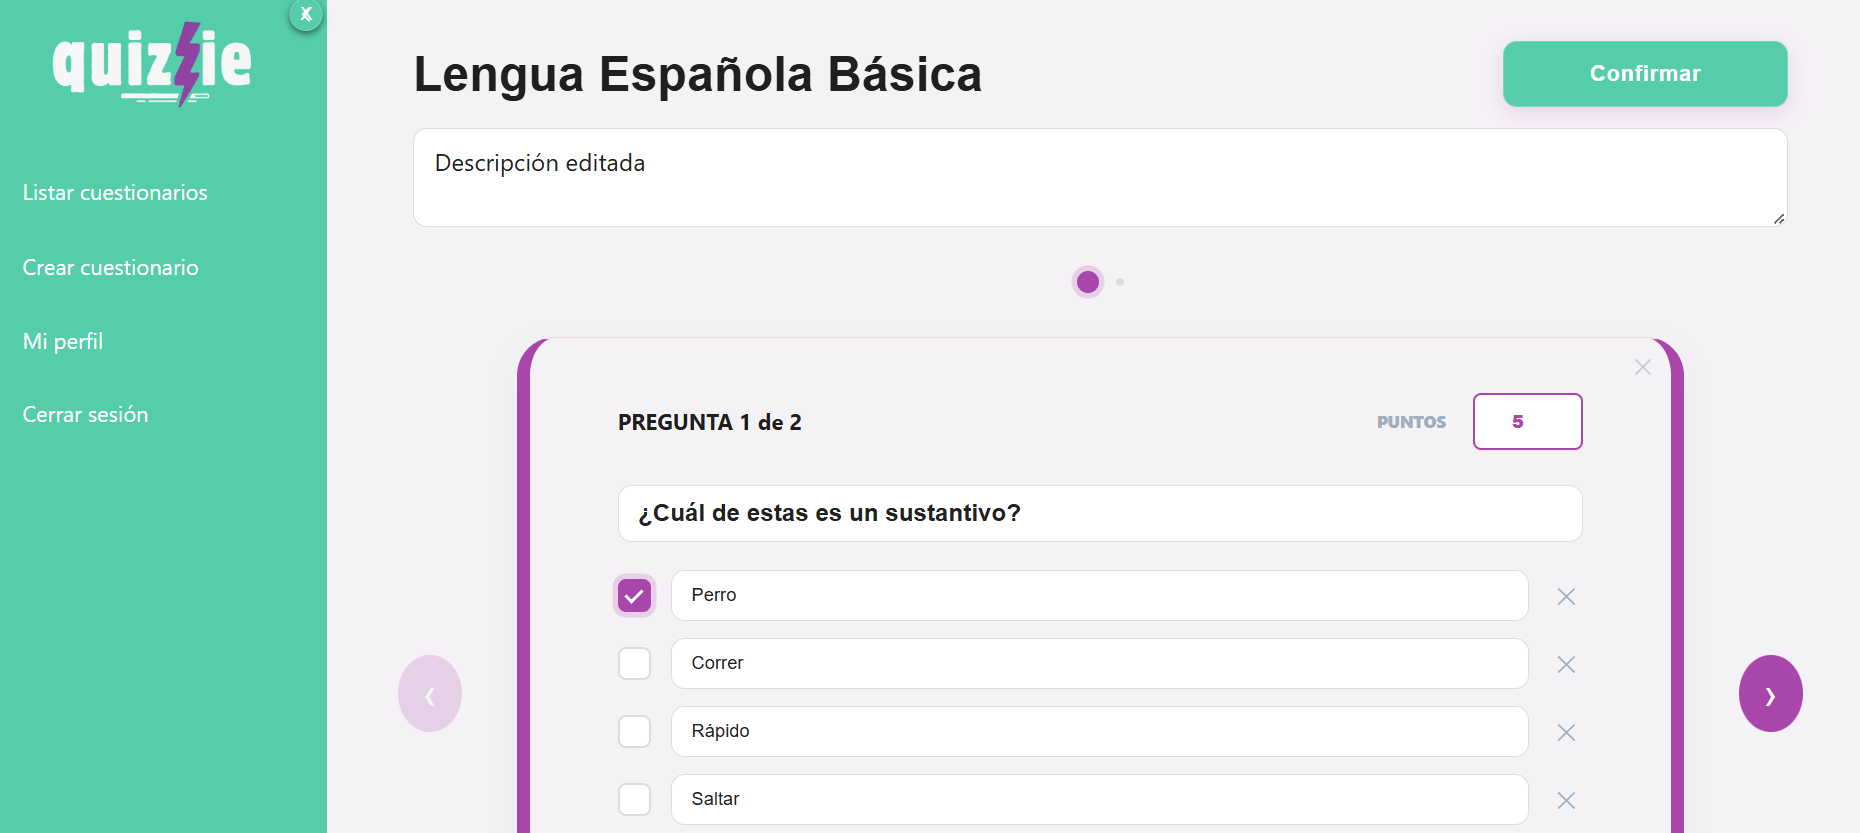
\includegraphics[width=1.1\textwidth]{screenshots/editar_cuestionario.png}%
  }
  \caption{Vista de edición de un cuestionario.}
  \label{fig:manual_editar_cuestionario}
\end{figure}

\subsection*{4. Historial de salas jugadas}

Al seleccionar la opción del ojo, el sistema presenta el registro histórico de las salas que se han disputado con dicho cuestionario. Al hacer clic sobre una sala concreta del listado, se accede al desglose pormenorizado de sus resultados.

\begin{figure}[H]
  \centering
  \makebox[\textwidth][c]{%
    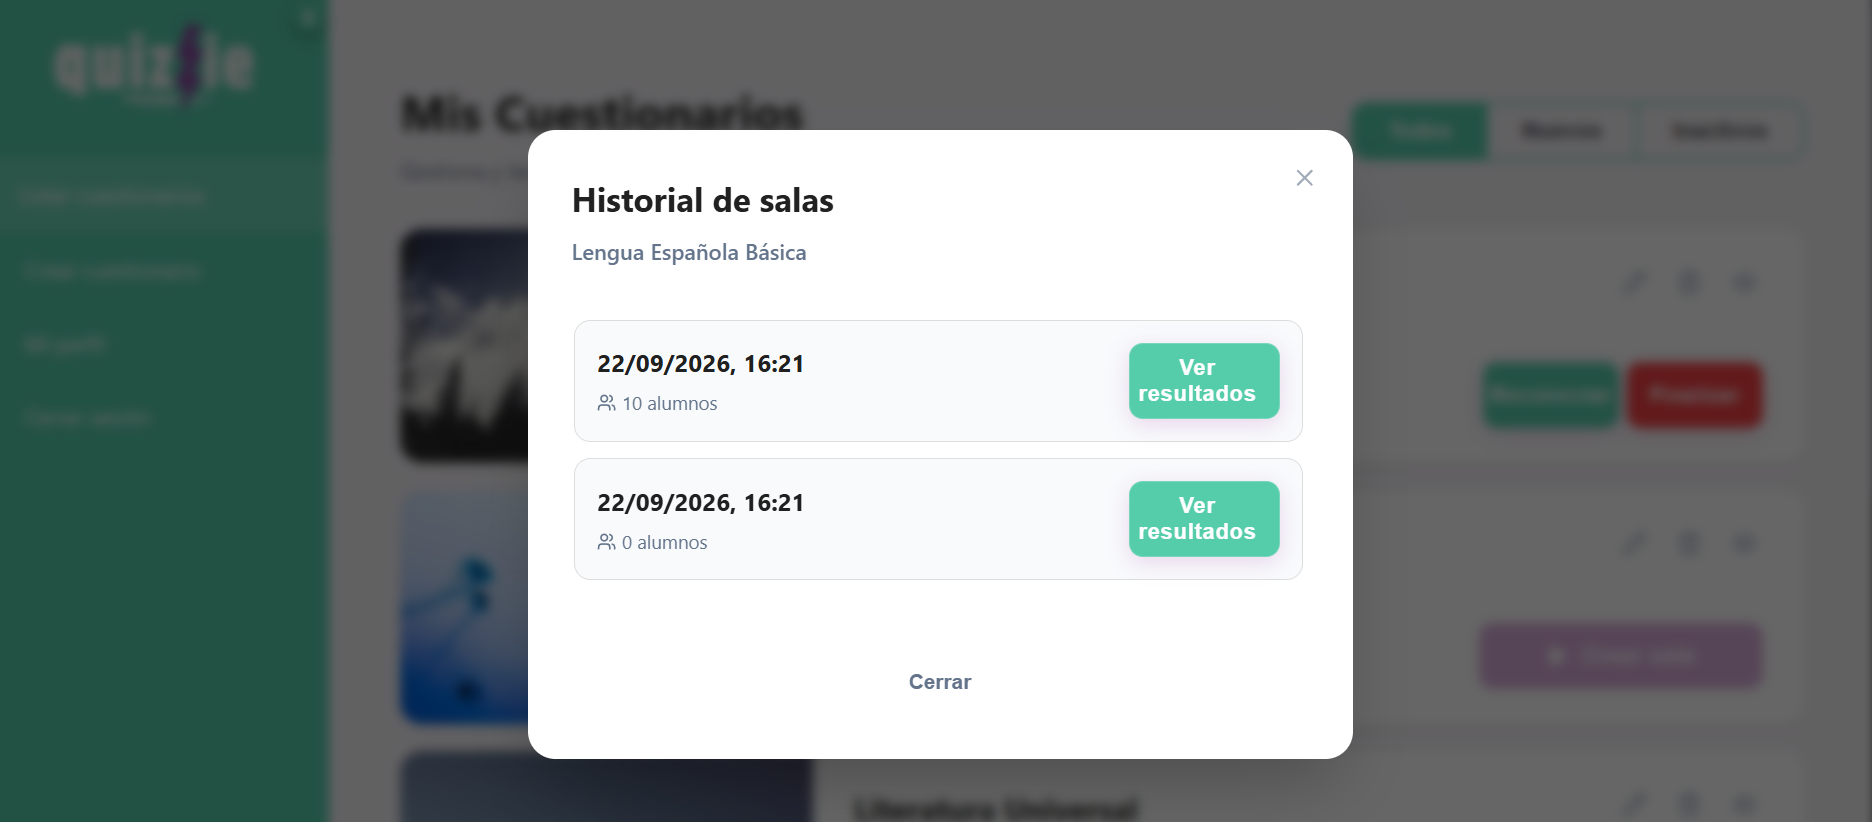
\includegraphics[width=1.1\textwidth]{screenshots/historial_salas.png}%
  }
  \caption{Historial de salas de un cuestionario.}
  \label{fig:manual_historial_salas}
\end{figure}

\subsection*{5. Detalle de resultados históricos y exportación}

En esta vista se muestran las puntuaciones registradas durante la sala seleccionada. Mediante el botón de descarga, el profesor puede exportar todo el conjunto de resultados a un archivo en formato CSV para su posterior tratamiento analítico o calificación externa.

\begin{figure}[H]
  \centering
  \makebox[\textwidth][c]{%
    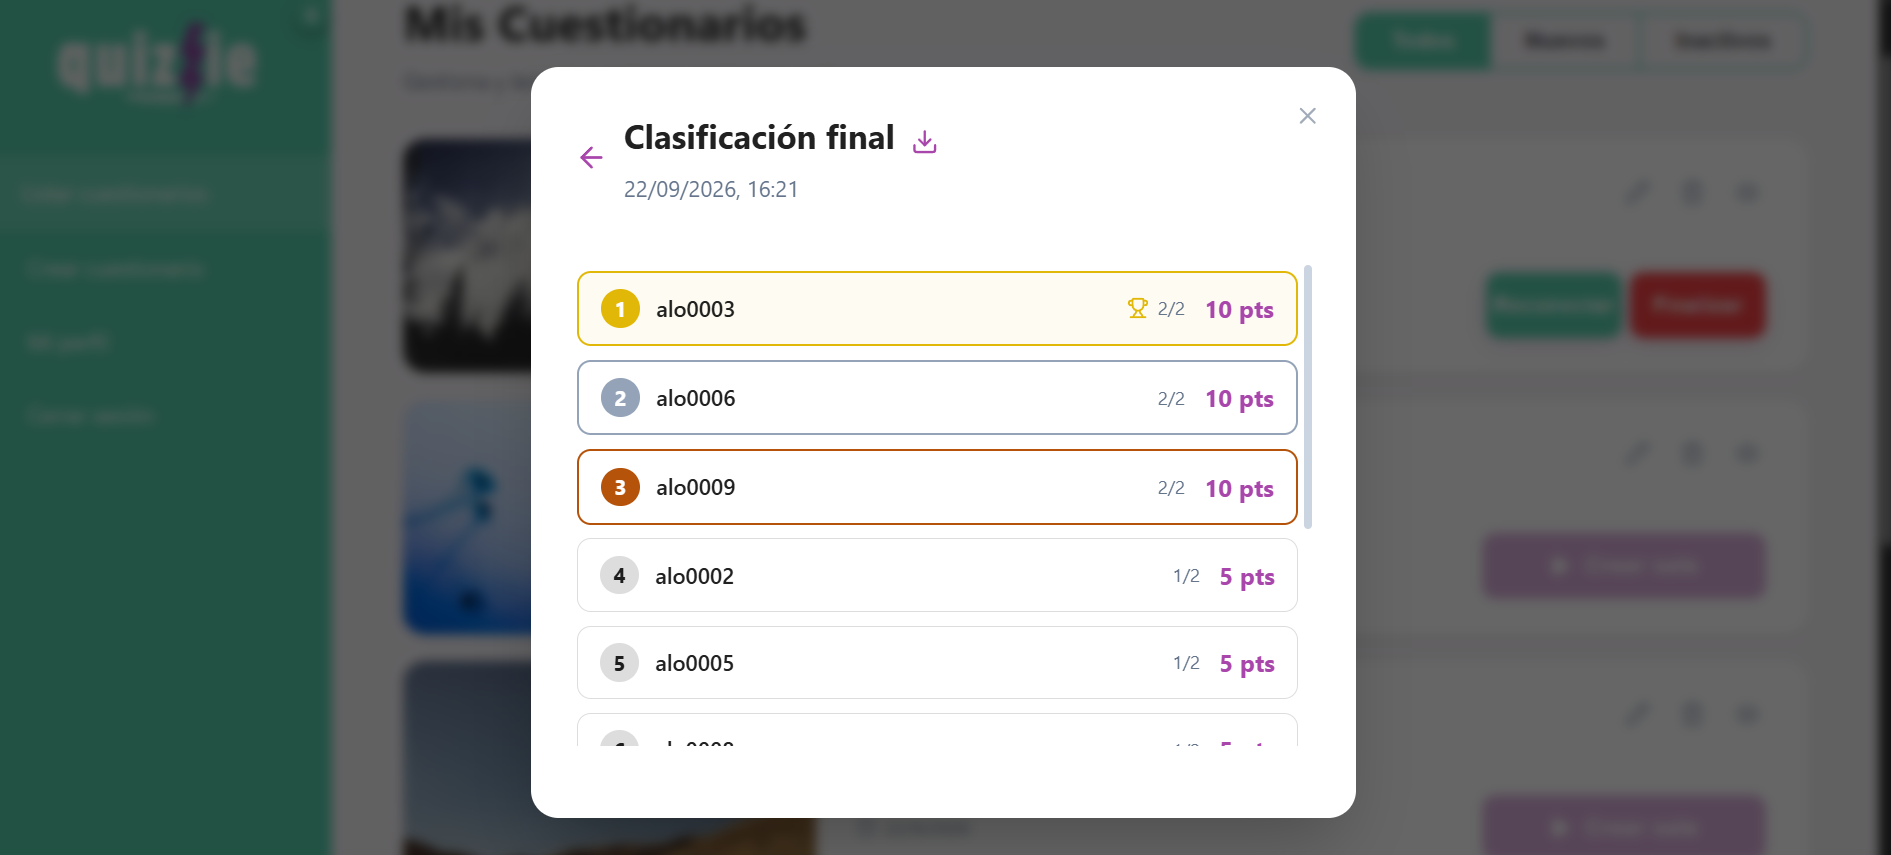
\includegraphics[width=1.1\textwidth]{screenshots/resultado_historico.png}%
  }
  \caption{Métricas detalladas de la sala y opción de exportación a CSV.}
  \label{fig:manual_resultado_historico}
\end{figure}

\subsection*{6. Eliminación de un cuestionario}

Al pulsar sobre el icono de la papelera, la plataforma solicita una confirmación previa para evitar pérdidas accidentales de datos antes de suprimir definitivamente el cuestionario.

\begin{figure}[H]
  \centering
  \makebox[\textwidth][c]{%
    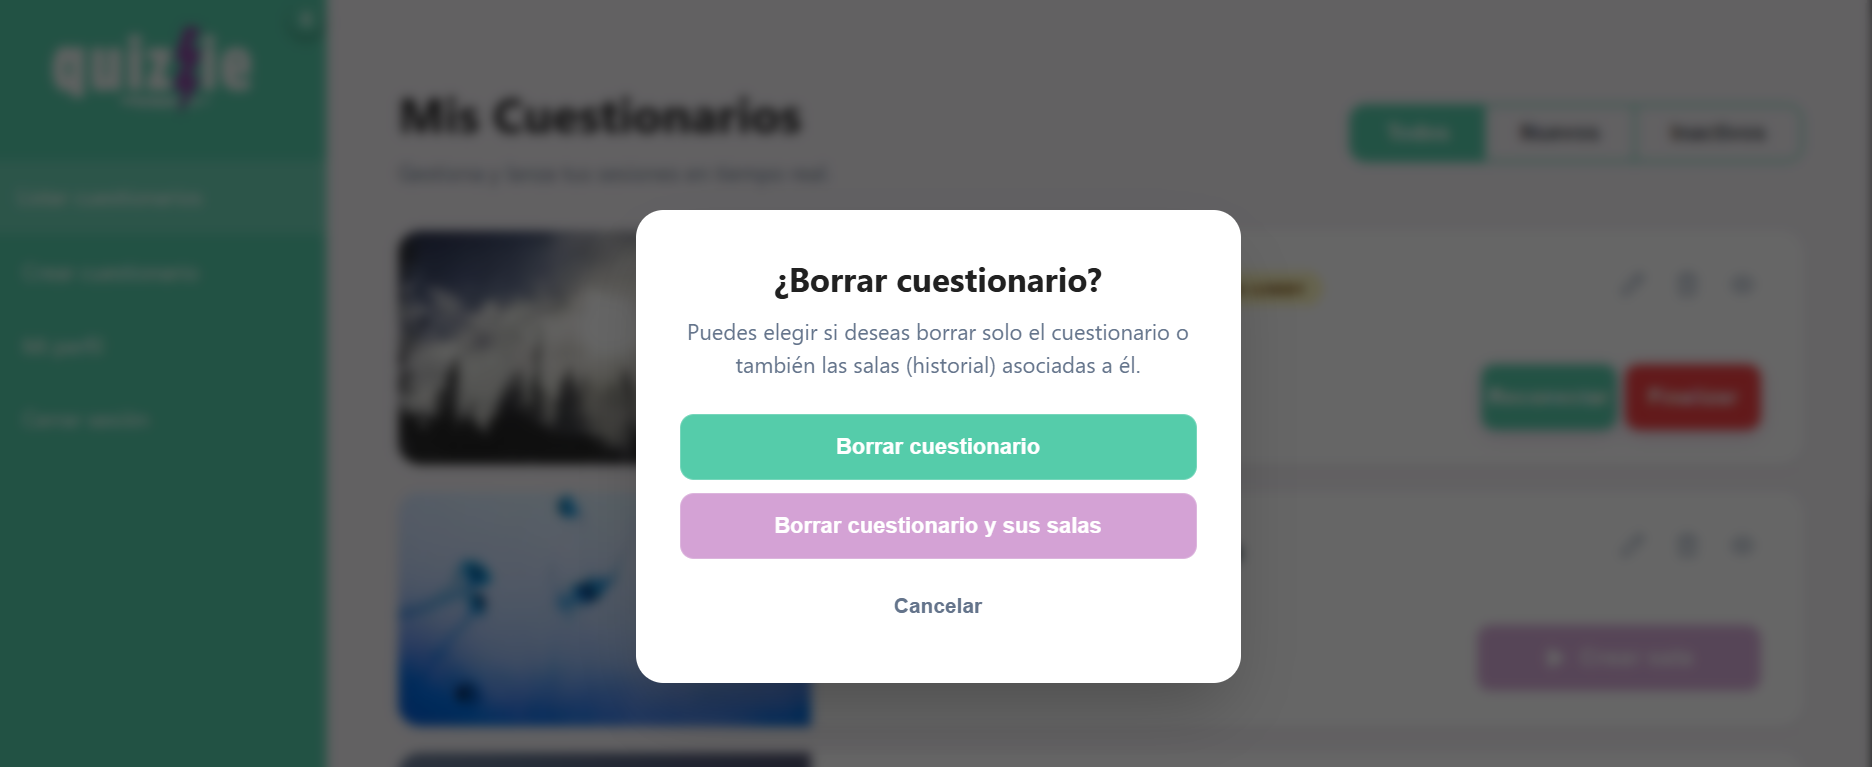
\includegraphics[width=1.1\textwidth]{screenshots/borrar_cuestionario.png}%
  }
  \caption{Diálogo de confirmación para eliminar un cuestionario.}
  \label{fig:manual_borrar_cuestionario}
\end{figure}

\subsection*{7. Creación de un nuevo cuestionario}

A través del botón de creación, el profesor accede a la interfaz de diseño de nuevos cuestionarios, donde define el título, las preguntas, las opciones de respuesta marcando la correcta y la puntuación máxima permitida.

\begin{figure}[H]
  \centering
  \makebox[\textwidth][c]{%
    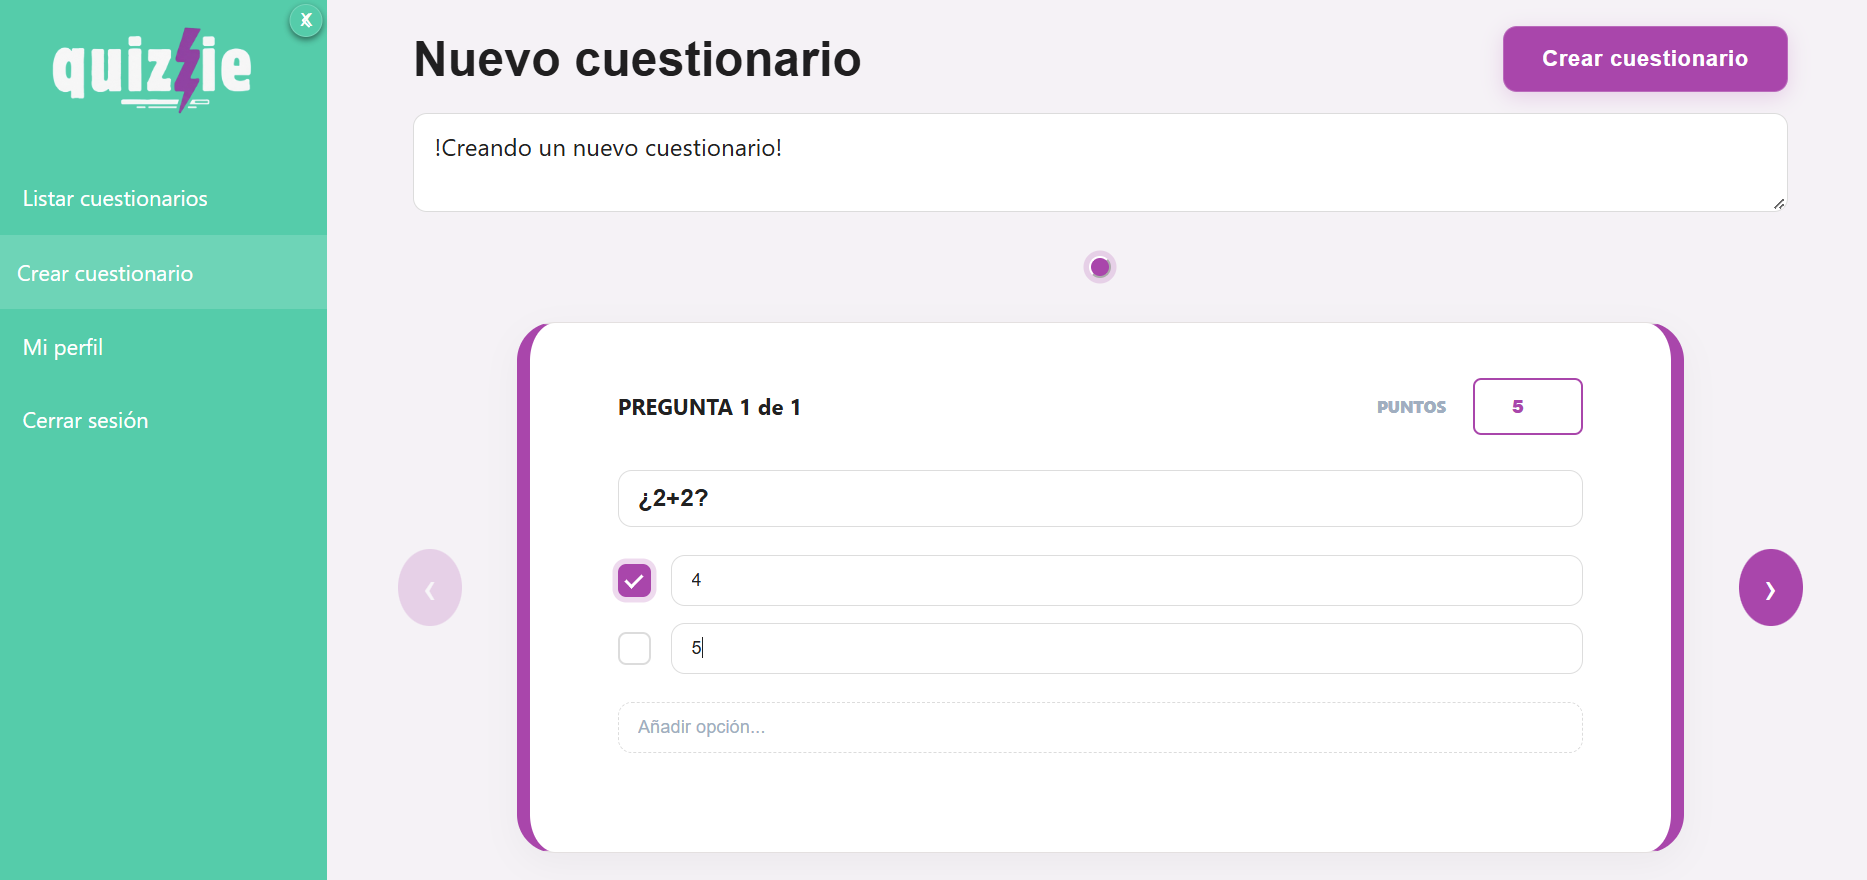
\includegraphics[width=1.1\textwidth]{screenshots/crear_cuestionario.png}%
  }
  \caption{Formulario para la creación de un nuevo cuestionario.}
  \label{fig:manual_crear_cuestionario}
\end{figure}

\subsection*{8. Visualización del catálogo filtrado}

Tras guardar los cambios, la nueva prueba queda registrada en el sistema y pasa a mostrarse dentro de la sección correspondiente en el catálogo de cuestionarios del usuario, lista para ser lanzada en una sala en directo.

\begin{figure}[H]
  \centering
  \makebox[\textwidth][c]{%
    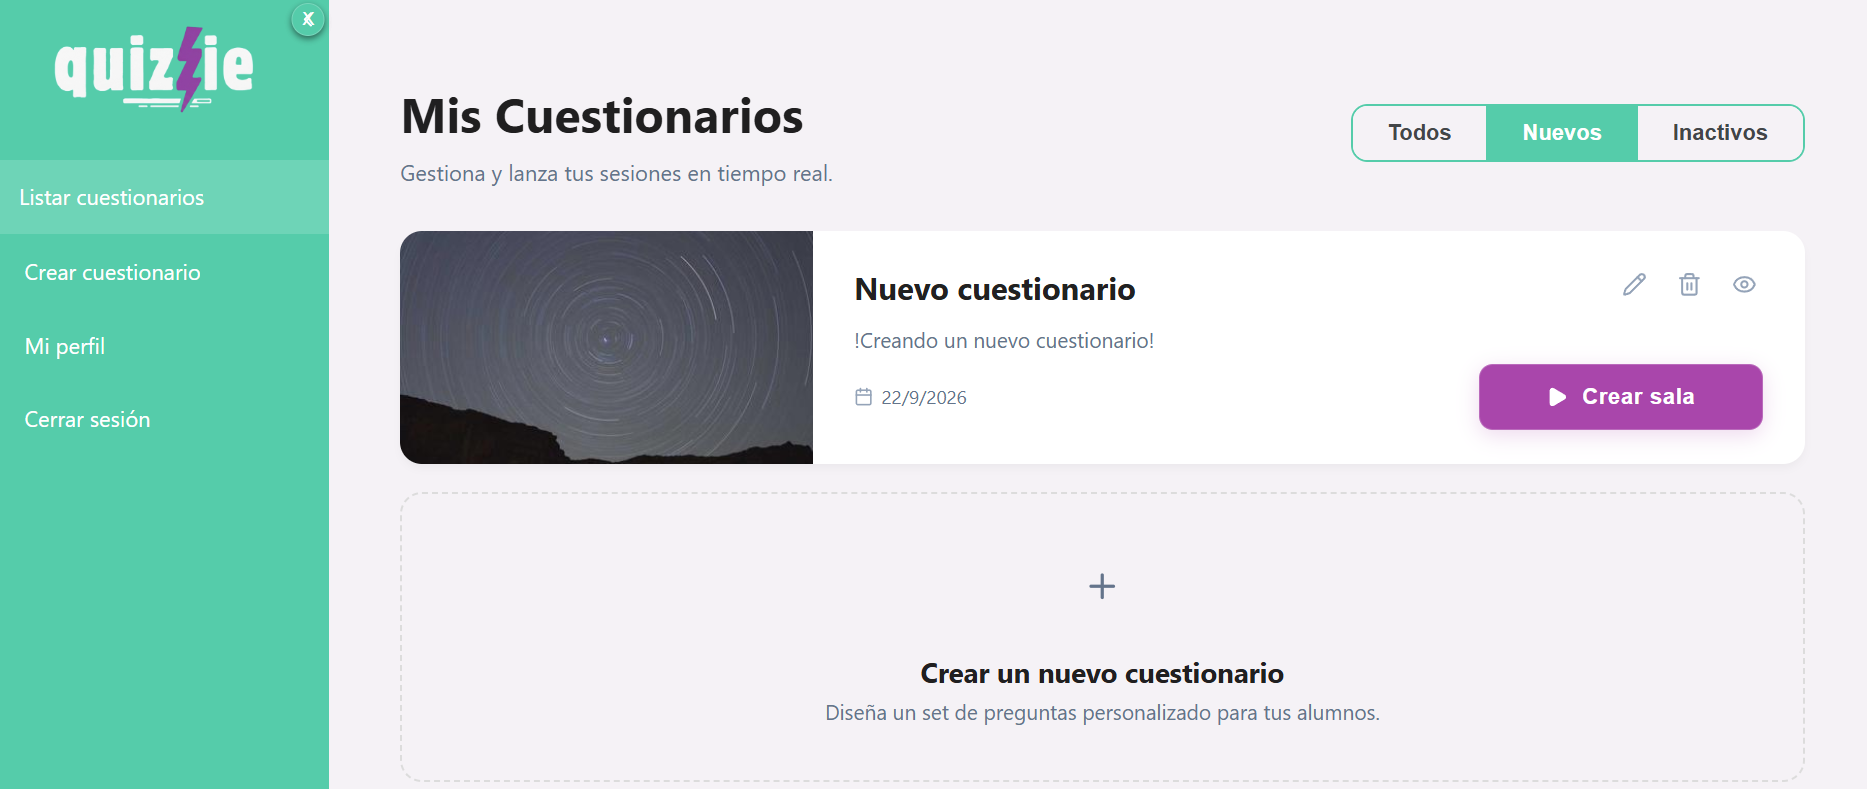
\includegraphics[width=1.1\textwidth]{screenshots/cuestionarios_nuevos.png}%
  }
  \caption{Cuestionario recién creado.}
  \label{fig:manual_cuestionarios_nuevos}
\end{figure}

\section*{Configuración, control de sala y verificación presencial}
\label{sec:manual_control_sala_en_directo}

Esta sección documenta el ciclo de vida completo de una sesión desde la perspectiva del profesor: desde el lanzamiento y parametrización de la sala, pasando por la orquestación de la partida en tiempo real, hasta la fase de verificación presencial mediante escaneo de códigos QR.

\subsection*{1. Selección de cuestionario y apertura de sala}

Desde la lista de cuestionarios, el profesor escoge la prueba que desea comenzar y pulsa sobre el botón para crear una nueva sala.

\begin{figure}[H]
  \centering
  \makebox[\textwidth][c]{%
    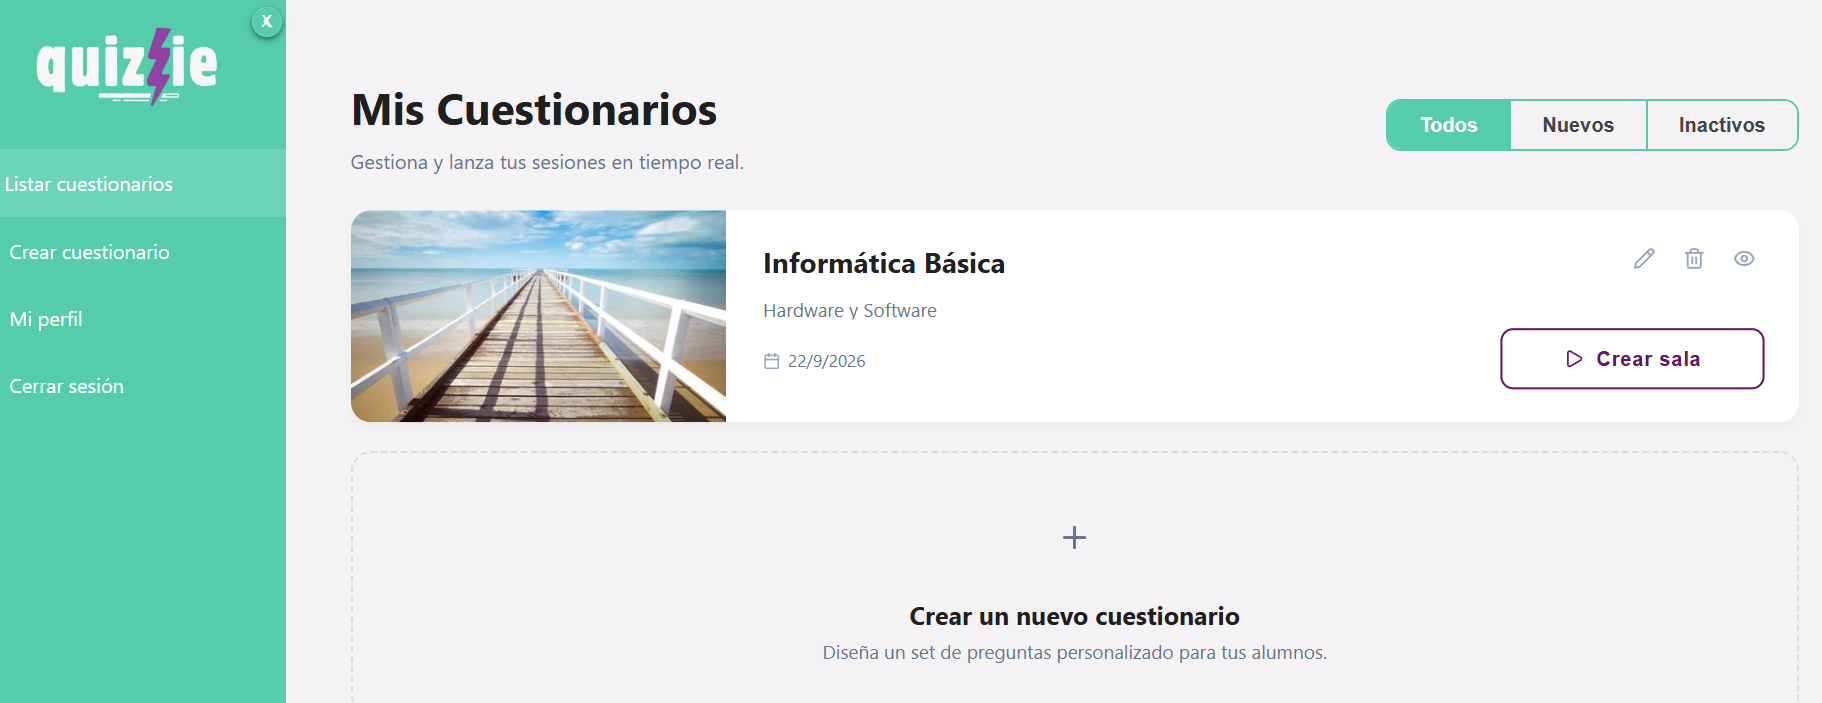
\includegraphics[width=1.1\textwidth]{screenshots/crear_sala.png}%
  }
  \caption{Selección de un cuestionario para inicializar una sala.}
  \label{fig:manual_crear_sala}
\end{figure}

\subsection*{2. Configuración de parámetros de la partida}

El profesor configura la dinámica de la partida a través de diversas opciones: orden aleatorio de preguntas, permutación aleatoria de opciones de respuesta para prevenir la copia entre estudiantes, visualización o no de rankings parciales tras cada pregunta (el ranking final siempre estará visible) y el tiempo límite concedido por pregunta. Al confirmar los parámetros, el sistema genera un código de acceso único y da paso a la sala de espera.

\begin{figure}[H]
  \centering
  \makebox[\textwidth][c]{%
    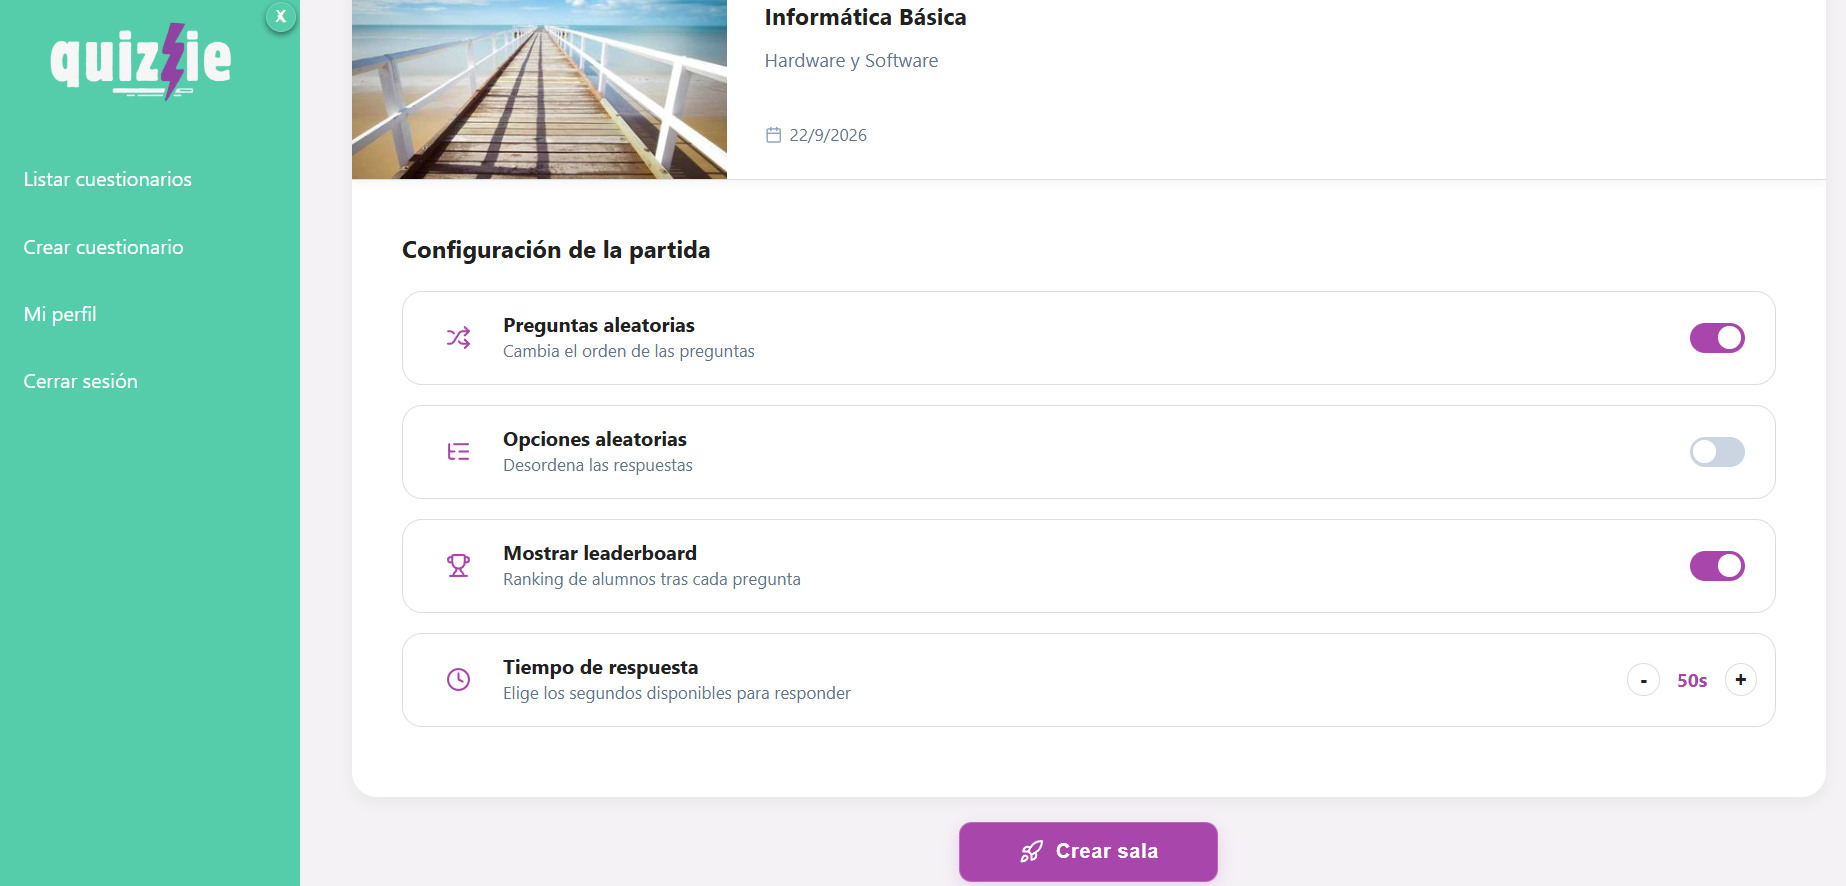
\includegraphics[width=1.1\textwidth]{screenshots/opciones_sala.png}%
  }
  \caption{Formulario de configuración de parámetros de la sala.}
  \label{fig:manual_opciones_sala}
\end{figure}

\subsection*{3. Sala de espera inicial}

La interfaz proyecta la sala de espera en su estado inicial vacío, exponiendo el código numérico PIN que el alumnado debe ingresar en sus dispositivos para vincularse a la sesión lectiva.

\begin{figure}[H]
  \centering
  \makebox[\textwidth][c]{%
    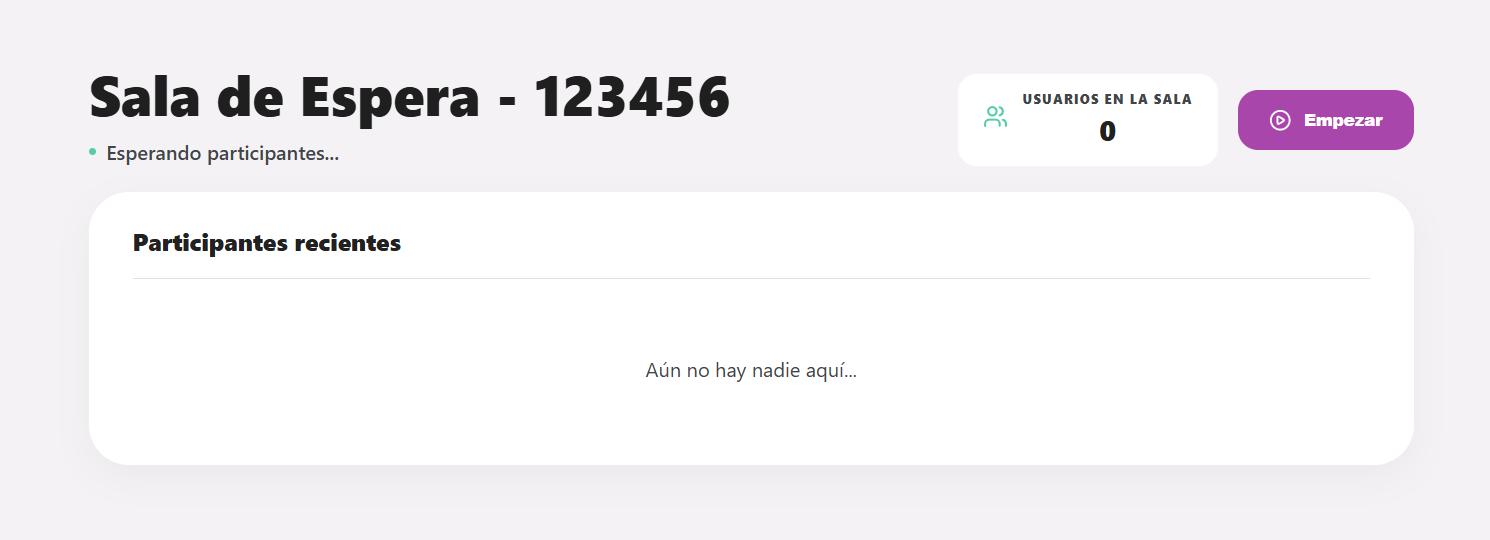
\includegraphics[width=1.1\textwidth]{screenshots/sala_espera_vacia.png}%
  }
  \caption{Sala de espera inicial a la espera de participantes.}
  \label{fig:manual_sala_espera_vacia}
\end{figure}

\subsection*{4. Incorporación de estudiantes y lanzamiento de la partida}

A medida que los estudiantes acceden a la sala, sus nombres o identificadores aparecen reflejados en pantalla. Cuando todos los asistentes se han incorporado, el profesor pulsa el botón para comenzar, dando paso a una breve cuenta atrás de sincronización previa al inicio de las preguntas.

\begin{figure}[H]
  \centering
  \makebox[\textwidth][c]{%
    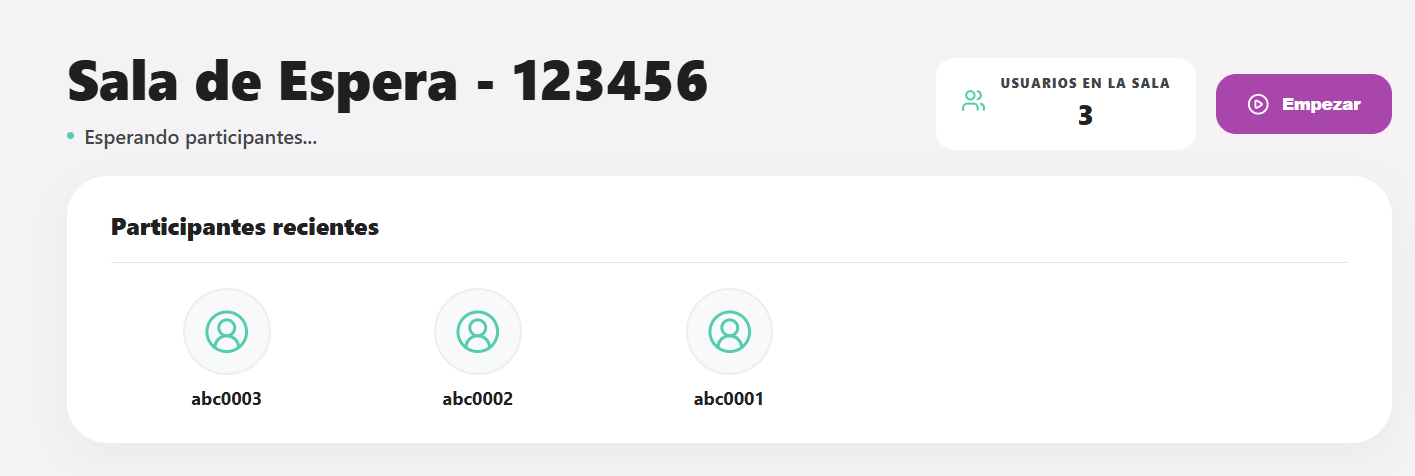
\includegraphics[width=1.1\textwidth]{screenshots/sala_espera.png}%
  }
  \caption{Sala de espera con estudiantes incorporados antes de iniciar.}
  \label{fig:manual_sala_espera}
\end{figure}

\subsection*{5. Fase de pregunta activa y recepción de respuestas}

Concluida la cuenta atrás, la plataforma proyecta el enunciado de la pregunta y el temporizador en cuenta regresiva según lo configurado. Los estudiantes solo pueden emitir respuestas mientras dicho reloj permanezca activo; si el temporizador se detiene o llega a cero, el sistema bloquea inmediatamente nuevos envíos.

\begin{figure}[H]
  \centering
  \makebox[\textwidth][c]{%
    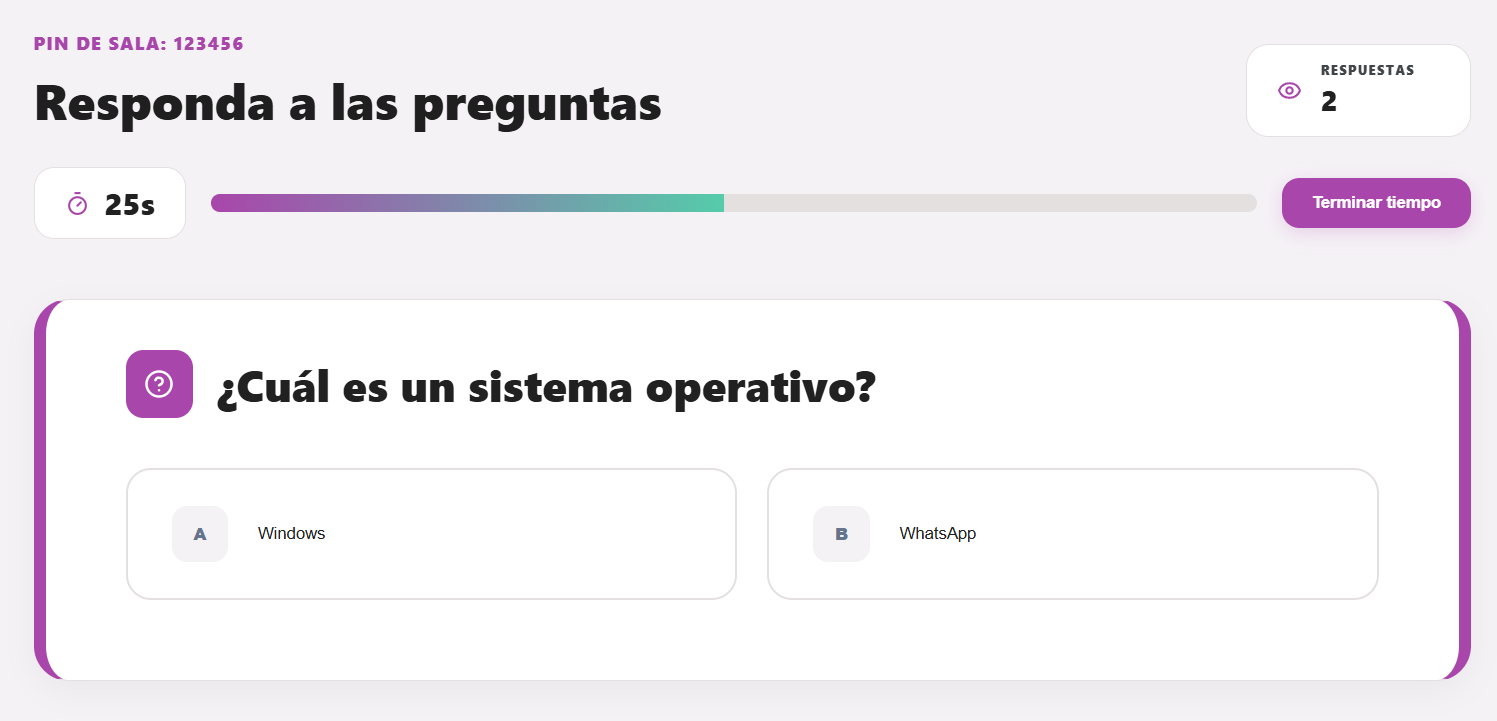
\includegraphics[width=1.1\textwidth]{screenshots/fase_respuesta_profesor.png}%
  }
  \caption{Pregunta proyectada en curso y temporizador activo.}
  \label{fig:manual_fase_respuesta_profesor}
\end{figure}

\subsection*{6. Tolerancia a fallos y reconexión del docente}

En caso de que el profesor sufra una pérdida de conexión de red o cierre accidentalmente la ventana, el sistema suspende de inmediato el temporizador para proteger la equidad de la prueba. Al volver a acceder a la plataforma, se ofrece la opción de reconexión directa a la sala activa, reanudándose el reloj y la interacción únicamente tras su regreso.

\begin{figure}[H]
  \centering
  \makebox[\textwidth][c]{%
    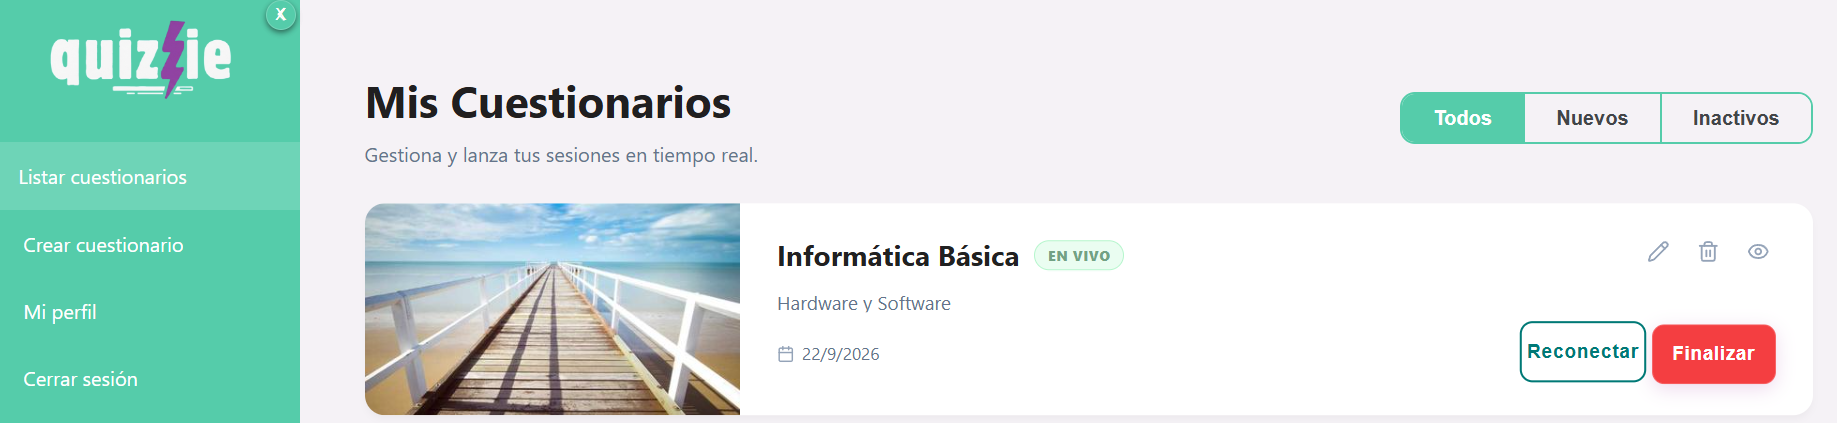
\includegraphics[width=1.1\textwidth]{screenshots/reconectarse_a_sala.png}%
  }
  \caption{Detección y recuperación de sesión activa tras desconexión.}
  \label{fig:manual_reconectarse_a_sala}
\end{figure}

\subsection*{7. Distribución analítica de respuestas}

Una vez agotado el tiempo de respuesta y al avanzar a la siguiente pantalla, el sistema proyecta una gráfica de barras con la distribución de las opciones elegidas por los alumnos. A partir de esta vista, y según las opciones configuradas inicialmente, se habilita la transición al ranking parcial o directamente a la siguiente pregunta o al final del cuestionario.

\begin{figure}[H]
  \centering
  \makebox[\textwidth][c]{%
    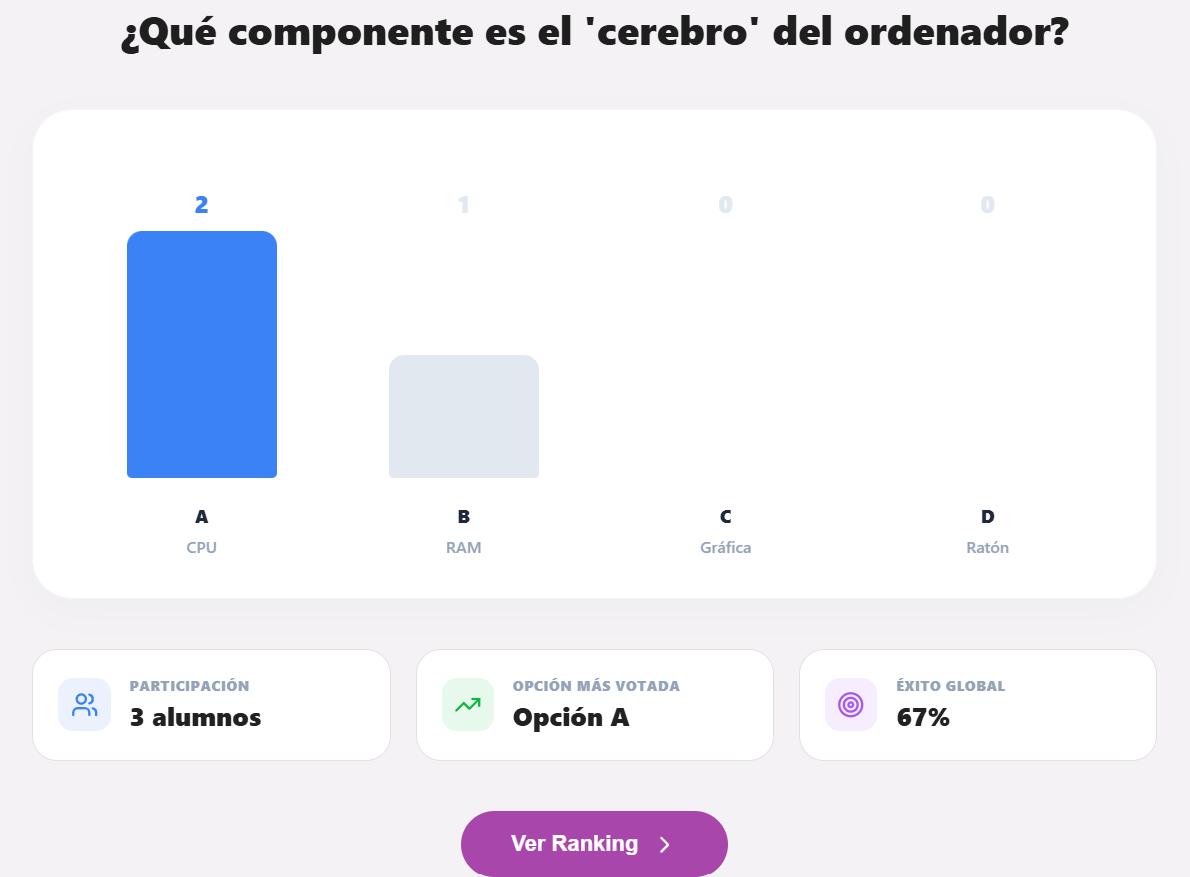
\includegraphics[width=0.9\textwidth]{screenshots/grafica_respuestas.png}%
  }
  \caption{Gráfica de distribución de respuestas seleccionadas por el alumnado.}
  \label{fig:manual_grafica_respuestas}
\end{figure}

\subsection*{8. Conclusión de la prueba y podio final}

Tras recorrer las rondas restantes de la evaluación, el sistema presenta la pantalla de podio final con las mejores calificaciones del aula. Al presionar el botón de finalización, la sala concluye su fase de preguntas y da paso al mecanismo de verificación presencial.

\begin{figure}[H]
  \centering
  \makebox[\textwidth][c]{%
    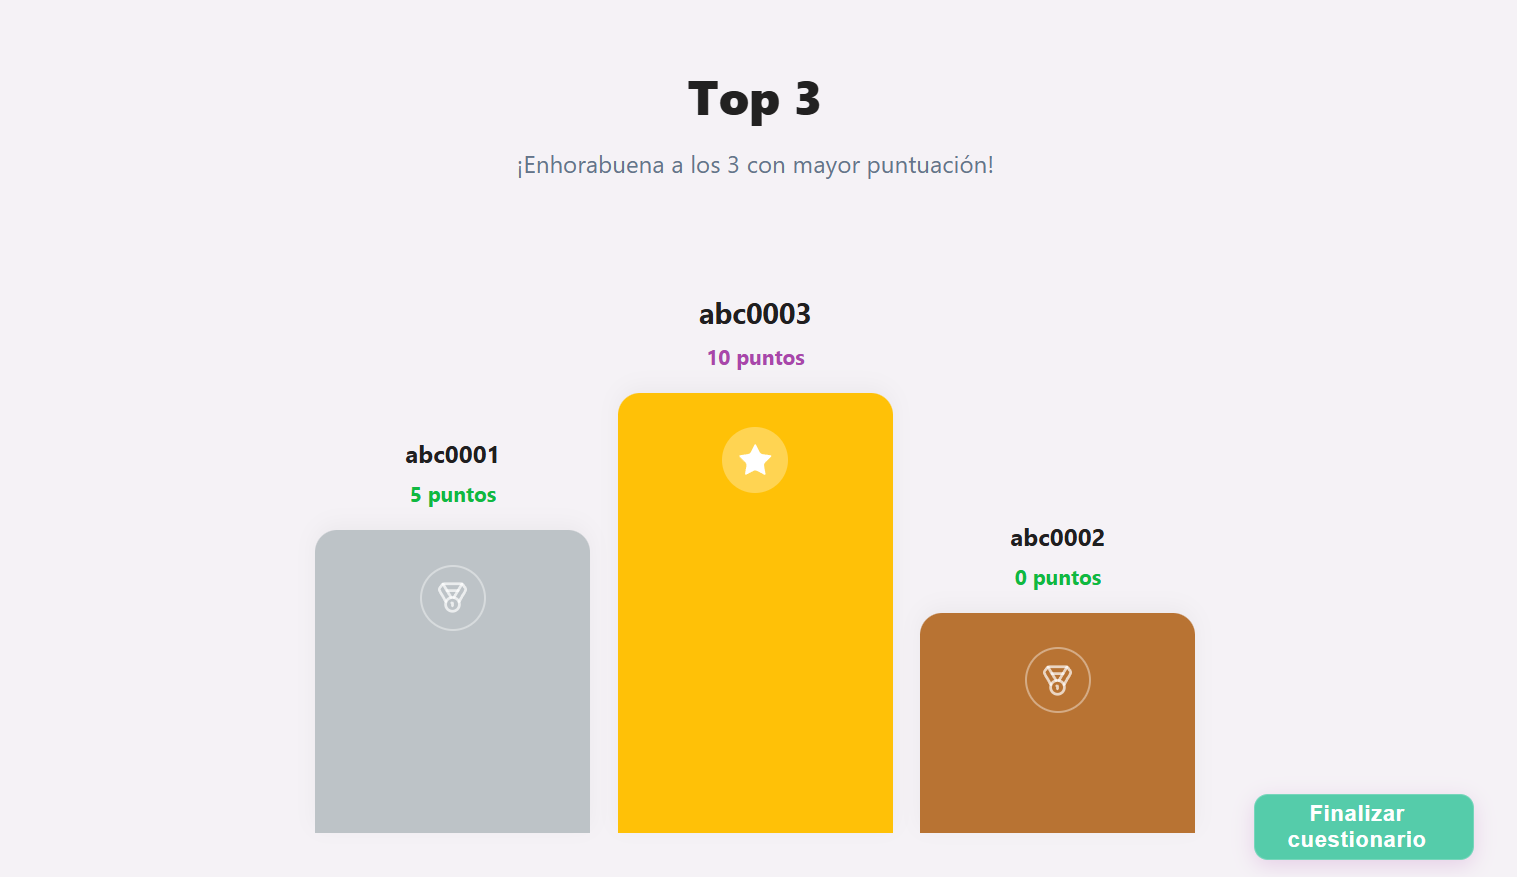
\includegraphics[width=0.9\textwidth]{screenshots/ranking_final.png}%
  }
  \caption{Podio de calificaciones globales al término de las preguntas.}
  \label{fig:manual_ranking_final}
\end{figure}

\subsection*{9. Panel de verificación presencial}

En esta fase, el profesor dispone de un panel con el listado de participantes para validar su asistencia física en el aula. Desde esta vista se habilita la acción para desplegar la interfaz de escaneo.

\begin{figure}[H]
  \centering
  \makebox[\textwidth][c]{%
    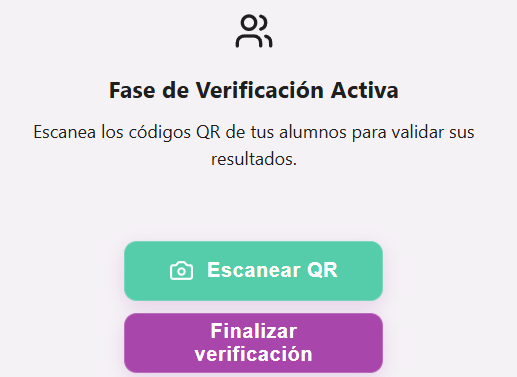
\includegraphics[width=0.55\textwidth]{screenshots/fase_verificacion.png}%
  }
  \caption{Panel para la verificación presencial de asistencia.}
  \label{fig:manual_fase_verificacion}
\end{figure}

\subsection*{10. Escáner y concesión de permisos de cámara}

Al solicitar la activación del lector de códigos, la aplicación despliega un diálogo modal que requiere la autorización del navegador para acceder a la cámara del dispositivo. Una vez concedido el permiso, el profesor procede al escaneo secuencial de los códigos QR mostrados en los dispositivos de los estudiantes para validar de forma fehaciente su presencialidad y asentar su nota.

\begin{figure}[H]
  \centering
  \makebox[\textwidth][c]{%
    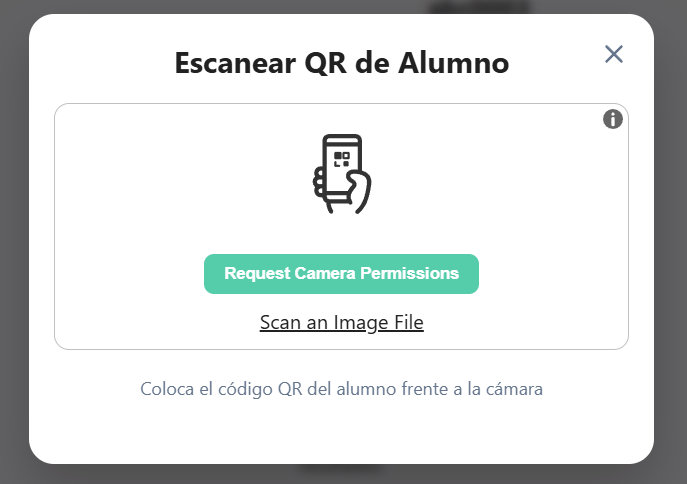
\includegraphics[width=0.6\textwidth]{screenshots/modal_verificacion.png}%
  }
  \caption{Diálogo modal de captura y solicitud de permisos de cámara.}
  \label{fig:manual_modal_verificacion}
\end{figure}

\end{appendices}
    \begin{appendices}

\chapter{Manual técnico}\label{anexo:manual_tecnico}

El presente manual técnico detalla el procedimiento para la clonación, configuración de dependencias, puesta en marcha del entorno de desarrollo local y reproducción íntegra de la batería de pruebas y análisis de rendimiento del sistema.

\section{Requisitos previos del sistema}\label{sec:manual_requisitos}

Para garantizar la correcta ejecución de la plataforma en un entorno local, la máquina anfitriona debe disponer de las herramientas base instaladas y registradas en las variables de entorno del sistema (\texttt{PATH}):

\begin{itemize}
    \item \textbf{Git}\cite{git_official}.
    \item \textbf{Node.js}\cite{nodejs_official}.
    \item \textbf{\texttt{uv}}\cite{uv_official} (puede instalarse nativamente o mediante \texttt{pip} si el sistema ya cuenta con un intérprete de Python).
\end{itemize}

\section{Preparación y configuración del repositorio}\label{sec:manual_preparacion}

\subsection*{Descarga del código fuente}
Clonar el repositorio del proyecto e ingresar en el directorio raíz:

\begin{lstlisting}
(*@\cliPrompt@*) (*@\bashYellow{git}@*) clone https://github.com/frangago71/quizzie-TFG.git
(*@\cliPrompt@*) (*@\bashYellow{cd}@*) quizzie-TFG
\end{lstlisting}

\subsection*{Configuración del entorno del backend}
Instalar el gestor \texttt{uv} en caso de no disponer de él previamente y sincronizar todas las dependencias del proyecto:

\begin{lstlisting}
(*@\cliPrompt@*) (*@\bashYellow{pip}@*) install uv
(*@\cliPrompt@*) (*@\bashYellow{uv}@*) sync (*@\bashGrey{--all-groups}@*)
\end{lstlisting}

La sincronización anterior genera un entorno virtual aislado (\texttt{.venv}) con todas las librerías necesarias. Para la ejecución de órdenes en dicho entorno se puede emplear el prefijo \texttt{uv run} en cada invocación, o bien activar explícitamente el entorno en la sesión de terminal para omitir dicho prefijo y ejecutar los comandos directamente:

\begin{lstlisting}
(*@\cliPrompt@*) (*@\bashYellow{\&}@*) .\.venv\Scripts\Activate.ps1
\end{lstlisting}

Para poblar la base de datos con los registros iniciales, acceder al directorio del backend y ejecutar el script de sembrado:

\begin{lstlisting}
(*@\cliPrompt@*) (*@\bashYellow{cd}@*) backend
(*@\cliPrompt@*) (*@\bashYellow{uv}@*) run python -m seed            (*@\covGreen{\# Ejecutar el sembrado inicial de datos}@*)
\end{lstlisting}

\subsection*{Configuración del entorno del frontend}
Acceder al directorio de la interfaz de usuario e instalar los módulos de dependencias:

\begin{lstlisting}
(*@\cliPrompt@*) (*@\bashYellow{cd}@*) ../frontend
(*@\cliPrompt@*) (*@\bashYellow{npm}@*) install                          (*@\covGreen{\# Instalar dependencias de Node.js}@*)
\end{lstlisting}

\subsection*{Configuración de variables de entorno}\label{subsec:manual_env}
Copiar la plantilla de configuración situada en la raíz del proyecto para generar el archivo local \texttt{.env}:

\begin{lstlisting}
(*@\cliPrompt@*) (*@\bashYellow{cp}@*) .env.example .env
\end{lstlisting}

A continuación, editar el archivo \texttt{.env} completando las siguientes secciones:

\begin{itemize}
    \item \textbf{\texttt{VITE\_API\_URL}}: Dirección base donde escucha la API de FastAPI. En local se establece en \texttt{http://localhost:8000}; en producción apuntará a la URL del backend desplegado.
    \item \textbf{\texttt{SECRET\_KEY}}: Clave simétrica utilizada para firmar criptográficamente los tokens de sesión. Para garantizar la seguridad, se recomienda generarla de manera aleatoria, por ejemplo ejecutando el siguiente comando en la terminal:
\begin{lstlisting}
(*@\cliPrompt@*) (*@\bashYellow{openssl}@*) rand -hex 32
\end{lstlisting}
    \item \textbf{\texttt{ALGORITHM}}: Algoritmo criptográfico de firma de tokens (por defecto, \texttt{HS256}).
    \item \textbf{\texttt{ACCESS\_TOKEN\_EXPIRE\_MINUTES}}: Tiempo de expiración del token de sesión expresado en minutos (fijado por defecto en 30).
    \item \textbf{\texttt{SMTP\_HOST}}: Nombre de dominio del servidor de correo saliente (por defecto, \texttt{smtp.gmail.com}).
    \item \textbf{\texttt{SMTP\_PORT}}: Puerto del servicio de transporte. Los valores habituales son \texttt{465} (cifrado implícito SSL) o \texttt{587} (cifrado explícito TLS/STARTTLS).
    \item \textbf{\texttt{SMTP\_USERNAME}}: Cuenta de correo electrónico empleada para la autenticación ante el servidor SMTP.
    \item \textbf{\texttt{SMTP\_PASSWORD}}: Clave de acceso al servicio. Al emplear Gmail, es indispensable utilizar una \textbf{Contraseña de aplicación} de Google generada desde la cuenta de seguridad, en lugar de la contraseña principal de usuario.
    \item \textbf{\texttt{SMTP\_FROM}}: Dirección visible en la cabecera del remitente. Si se omite, toma automáticamente el valor de \texttt{SMTP\_USERNAME}. En servidores como Gmail, este campo debe coincidir con la cuenta autenticada para evitar que el servidor rechace el envío por sospecha de suplantación.
    \item \textbf{\texttt{GEMINI\_API\_KEY}}: Clave de acceso a la API de Google Gemini para la generación asistida de cuestionarios. Corresponde a una funcionalidad planificada para la siguiente etapa y que queda fuera del alcance de la presente entrega del TFG.
\end{itemize}

El archivo \texttt{.env} resultante se encuentra excluido mediante el archivo \texttt{.gitignore}, garantizando que ninguna credencial privada alcance el repositorio remoto.

\section{Ejecución del proyecto en el entorno local}\label{sec:manual_ejecucion}

La plataforma requiere la ejecución simultánea de dos procesos independientes. Para ello, se recomienda disponer de dos terminales de trabajo activas de manera concurrente.

\subsection*{Terminal 1: Servicio del backend (FastAPI)}
Iniciar el servidor de desarrollo del \textit{backend}:

\begin{lstlisting}
(*@\cliPrompt@*) (*@\bashYellow{cd}@*) backend
(*@\cliPrompt@*) (*@\bashYellow{uv}@*) run fastapi dev        
\end{lstlisting}

Una vez levantado el servicio, los accesos locales quedan disponibles en:
\begin{itemize}
    \item \texttt{http://127.0.0.1:8000}: Raíz del servidor y servicio de la API.
    \item \texttt{http://127.0.0.1:8000/docs}: Documentación - \textbf{Swagger UI}.
    \item \texttt{http://127.0.0.1:8000/redoc}: Documentación - \textbf{ReDoc}.
\end{itemize}

\subsection*{Terminal 2: Cliente del frontend (Vite)}
Acceder al directorio de la interfaz y levantar el servidor de desarrollo local:

\begin{lstlisting}
(*@\cliPrompt@*) (*@\bashYellow{cd}@*) frontend
(*@\cliPrompt@*) (*@\bashYellow{npm}@*) run dev               
\end{lstlisting}

La interfaz web quedará accesible desde el navegador en \texttt{http://localhost:5173}.

\section{Procedimiento de ejecución de pruebas y cobertura}\label{sec:manual_pruebas}

\subsection*{Pruebas unitarias y de integración del \textit{backend}}

Ejecutar la suite completa de pruebas unitarias y de integración del \textit{backend} mediante \texttt{pytest}:

\begin{lstlisting}
(*@\cliPrompt@*) (*@\bashYellow{uv}@*) run pytest
\end{lstlisting}

Para auditar la cobertura de código y generar reportes adicionales, se pueden combinar los siguientes modificadores:

\begin{itemize}
    \item \texttt{--cov=backend}: Delimita el análisis exclusivamente al código fuente del \textit{backend}.
    \item \texttt{--cov-report=term-missing}: Imprime en la consola la tabla desglosada por módulo señalando las líneas exactas sin cobertura.
    \item \texttt{--cov-report=html}: Genera un informe visual interactivo estructurado dentro del directorio local \texttt{htmlcov/}.
\end{itemize}

Al combinar estas tres opciones, se imprime en la terminal la tabla de cobertura del \textit{backend} y se genera un informe interactivo en \texttt{htmlcov/index.html}:

\begin{lstlisting}
(*@\cliPrompt@*) (*@\bashYellow{uv}@*) run pytest (*@\bashGrey{--cov=backend --cov-report=term-missing --cov-report=html}@*)
\end{lstlisting}

\begin{evidence}[H]
    \centering
    \makebox[\textwidth][c]{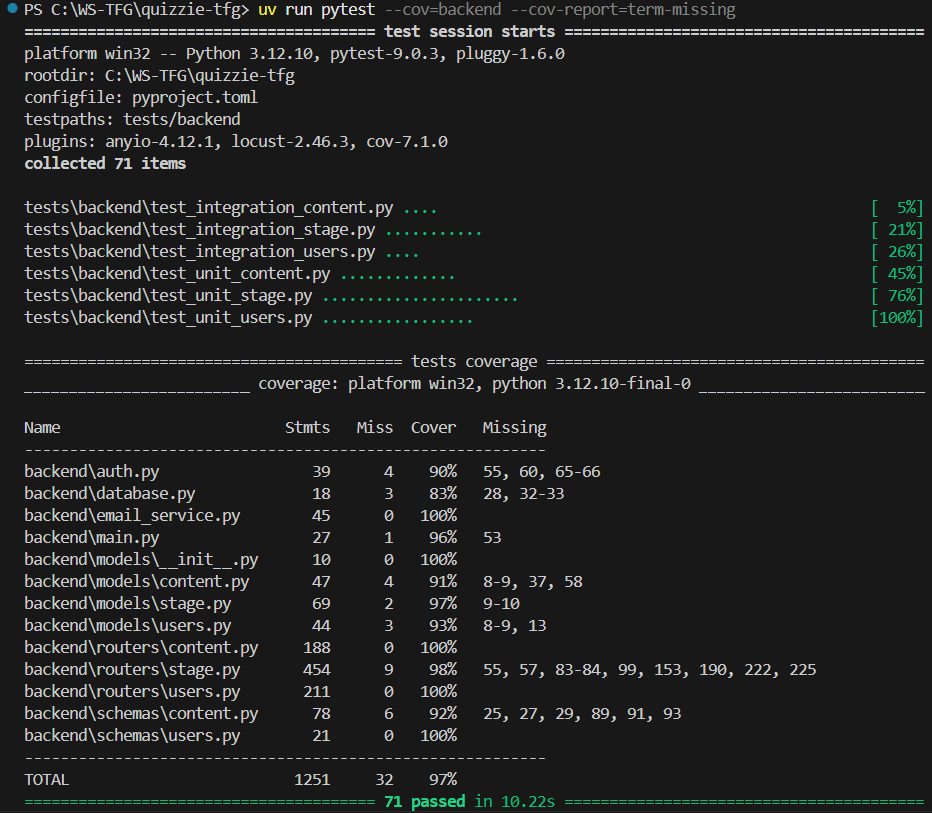
\includegraphics[width=0.82\textwidth]{evidences/terminal_test_backend.png}}
    \captionsetup{hypcap=false}
    \caption*{Salida por terminal al ejecutar las pruebas y la cobertura del \textit{backend}.}
\end{evidence}

Para abrir el reporte web directamente en el navegador predeterminado desde la consola según el sistema operativo:

\begin{lstlisting}
(*@\cliPrompt@*) (*@\bashYellow{start}@*) htmlcov/index.html                  (*@\covGreen{\# Windows}@*)
(*@\cliPrompt@*) (*@\bashYellow{xdg-open}@*) htmlcov/index.html                 (*@\covGreen{\# Linux}@*)
(*@\cliPrompt@*) (*@\bashYellow{open}@*) htmlcov/index.html                     (*@\covGreen{\# macOS}@*)
\end{lstlisting}

De manera alternativa, el informe puede consultarse abriendo el archivo a través del explorador del sistema operativo.

\subsection*{Pruebas de componentes del \textit{frontend}}

Acceder al directorio de la interfaz y ejecutar la suite completa de pruebas unitarias y de componentes:

\begin{lstlisting}
(*@\cliPrompt@*) (*@\bashYellow{cd}@*) frontend
(*@\cliPrompt@*) (*@\bashYellow{npm}@*) run test
\end{lstlisting}

Ejecutar la suite de pruebas evaluando la cobertura de código:

\begin{lstlisting}
(*@\cliPrompt@*) (*@\bashYellow{npm}@*) run test:frontend:coverage
\end{lstlisting}

Al ejecutar este comando, se imprime por terminal el desglose cuantitativo de cobertura acotado a los módulos clave (\texttt{auth}, \texttt{management}, \texttt{room-access} y \texttt{room-play}) y se genera el directorio de cobertura \texttt{frontend/coverage/}:

\begin{evidence}[H]
    \centering
    \makebox[\textwidth][c]{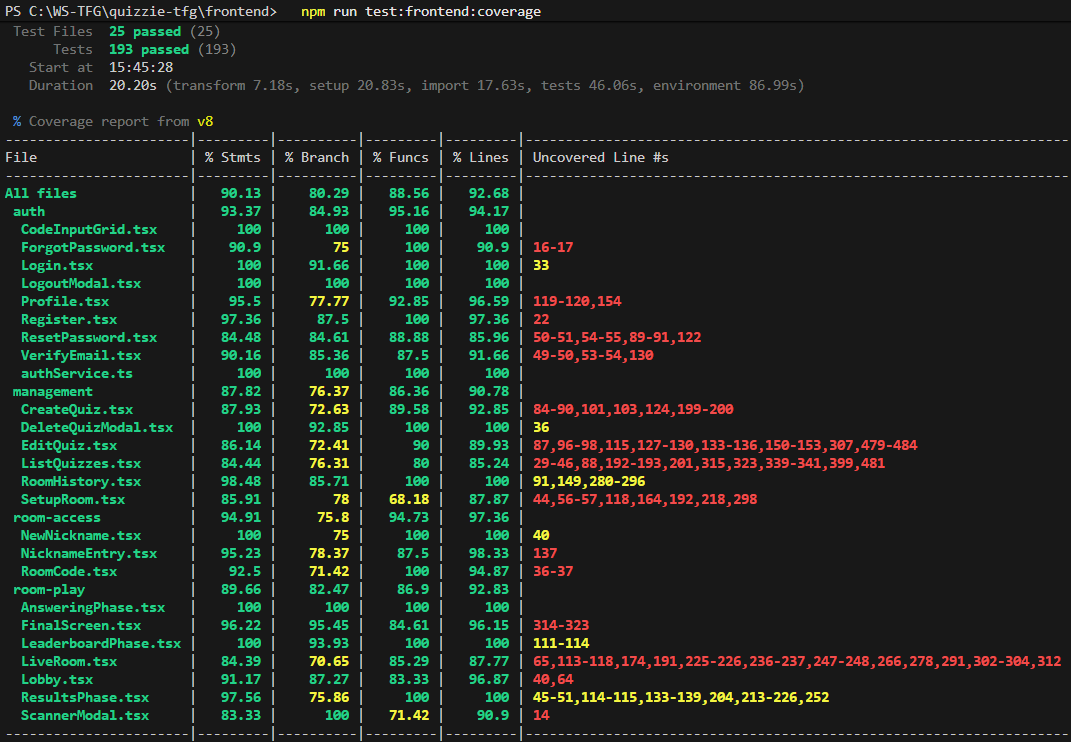
\includegraphics[width=\textwidth]{evidences/terminal_test_componentes.png}}
    \captionsetup{hypcap=false}
    \caption*{Salida por terminal al ejecutar las pruebas y la cobertura de componentes.}
\end{evidence}

Para visualizar en el navegador el informe web interactivo generado, iniciar el servidor local de visualización:

\begin{lstlisting}
(*@\cliPrompt@*) (*@\bashYellow{npm}@*) run cov-report:frontend
\end{lstlisting}

El reporte web queda desplegado en \texttt{http://localhost:4173}. Asimismo, es posible visualizarlo de forma estática cargando \texttt{frontend/coverage/index.html} en el navegador.

\subsection*{Pruebas de extremo a extremo y cobertura E2E}

Ejecutar la suite de pruebas \textit{End-to-End} sobre la compilación de producción del cliente web:

\begin{lstlisting}
(*@\cliPrompt@*) (*@\bashYellow{cd}@*) frontend
(*@\cliPrompt@*) (*@\bashYellow{npm}@*) run test:e2e
\end{lstlisting}

Al finalizar la ejecución, la consola muestra el resumen de los escenarios evaluados y se generan los informes de trazas de ejecución de casos de uso y de cobertura:

\begin{evidence}[H]
    \centering
    \makebox[\textwidth][c]{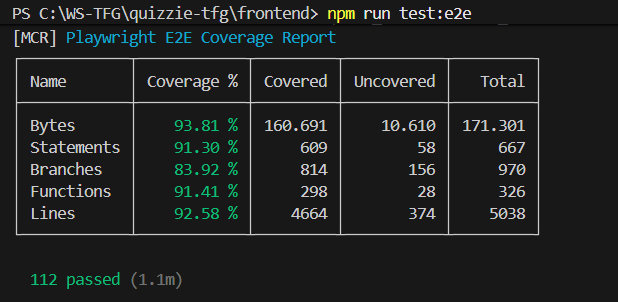
\includegraphics[width=0.85\textwidth]{evidences/terminal_test_e2e.png}}
    \captionsetup{hypcap=false}
    \caption*{Salida por terminal al ejecutar las pruebas de extremo a extremo.}
\end{evidence}

Para inspeccionar las trazas detalladas, capturas de pantalla y pasos de ejecución mediante el servidor integrado de Playwright:

\begin{lstlisting}
(*@\cliPrompt@*) (*@\bashYellow{npx}@*) playwright show-report
\end{lstlisting}

El reporte queda desplegado en \texttt{http://localhost:9323}, permaneciendo almacenado como archivo estático en \texttt{frontend/playwright-report/index.html}.

Para previsualizar el informe de cobertura interactivo generado por \textbf{Monocart}, levantar el servidor local:

\begin{lstlisting}
(*@\cliPrompt@*) (*@\bashYellow{npm}@*) run cov-report:e2e
\end{lstlisting}

El reporte queda accesible en \texttt{http://localhost:4174}, o bien abriendo directamente el archivo \texttt{frontend/coverage-e2e/index.html}.

\subsection*{Pruebas de carga y rendimiento}

Para ejecutar estas pruebas es necesario disponer de dos terminales abiertas: una manteniendo el servicio del \textit{backend} en ejecución en \texttt{http://127.0.0.1:8000} y otra situada en la raíz del proyecto para lanzar las pruebas.

El flujo de trabajo se compone de dos fases: en primer lugar, se inyecta la carga en el servidor mediante Locust, lo que genera automáticamente los registros de métricas en formato CSV dentro del directorio \texttt{tests/locust/}. Posteriormente, el script \texttt{tests/locust/evaluate\_thresholds.py} procesa dichos ficheros para verificar si los tiempos de respuesta y las tasas de error se mantienen dentro de los umbrales de aceptación definidos.

Para llevar a cabo la inyección de carga se dispone de dos alternativas válidas:

\subsubsection*{Opción 1: Modo interactivo con interfaz web}

Iniciar el panel gráfico de control de Locust para configurar los parámetros manualmente y monitorizar la prueba en tiempo real en \texttt{http://localhost:8089}:

\begin{lstlisting}[basicstyle=\fontsize{11.5pt}{13.2pt}\ttfamily\color{black}, aboveskip=4pt, belowskip=4pt]
(*@\cliPrompt@*) (*@\bashYellow{uv}@*) run locust -f tests/locust/locustfile.py --host http://127.0.0.1:8000
\end{lstlisting}

\subsubsection*{Opción 2: Ejecución por consola}

Ejecutar las pruebas directamente desde la terminal utilizando el script automatizado con la configuración base (200 usuarios, tasa de 15~u/s y 1~minuto de duración):

\begin{lstlisting}
(*@\cliPrompt@*) (*@\bashYellow{uv}@*) run python tests/locust/run_performance_tests.py
\end{lstlisting}

Para personalizar las condiciones de estrés, es posible sobrescribir estos valores mediante los siguientes argumentos:

\begin{lstlisting}
(*@\cliPrompt@*) (*@\bashYellow{uv}@*) run python tests/locust/run_performance_tests.py (*@\bashGrey{-u}@*) 300 (*@\bashGrey{-r}@*) 25 (*@\bashGrey{-t}@*) 2m
\end{lstlisting}

\begin{itemize}
    \item \texttt{-u} (\texttt{--users}): Número de usuarios virtuales simultáneos.
    \item \texttt{-r} (\texttt{--spawn-rate}): Tasa de incorporación de nuevos usuarios por segundo.
    \item \texttt{-t} (\texttt{--run-time}): Duración total de la prueba.
    \item \texttt{--host}: Dirección base del servicio \textit{backend}.
\end{itemize}

Una vez concluida la prueba mediante cualquiera de las dos alternativas y generados los archivos CSV, ejecutar el script de auditoría para verificar cuantitativamente el cumplimiento de los umbrales de aceptación:

\begin{lstlisting}
(*@\cliPrompt@*) (*@\bashYellow{uv}@*) run python tests/locust/evaluate_thresholds.py
\end{lstlisting}

\newpage

Al procesar los registros, la herramienta contrasta las latencias y tasas de error frente a los límites admisibles:

\begin{evidence}[H]
    \centering
    \makebox[\textwidth][c]{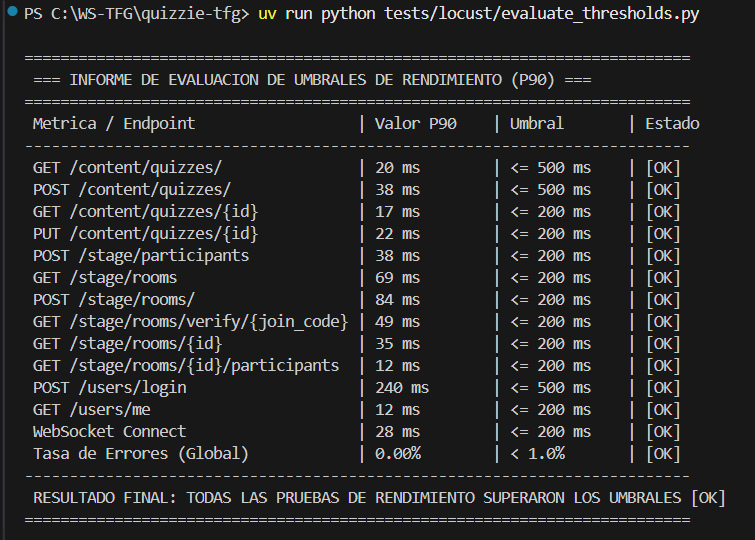
\includegraphics[width=0.85\textwidth]{evidences/terminal_test_umbrales.png}}
    \captionsetup{hypcap=false}
    \caption*{Salida por terminal del \textit{script} de cumplimiento de umbrales.}
\end{evidence}

\end{appendices}
    \begin{appendices}
\chapter{Registro de pruebas y cobertura}\label{anexo:registro_pruebas_cobertura}

Resultados de pruebas con cobertura
\end{appendices}
    \begin{appendices}
\chapter{Informe de dedicación temporal con \textit{Clockify}}\label{anexo:clockify}

En este anexo se adjunta el informe completo de seguimiento temporal exportado directamente de la herramienta Clockify, donde se detalla el cómputo de horas imputadas a cada una de las tareas del proyecto y sus correspondientes etiquetas de vinculación con las actividades.

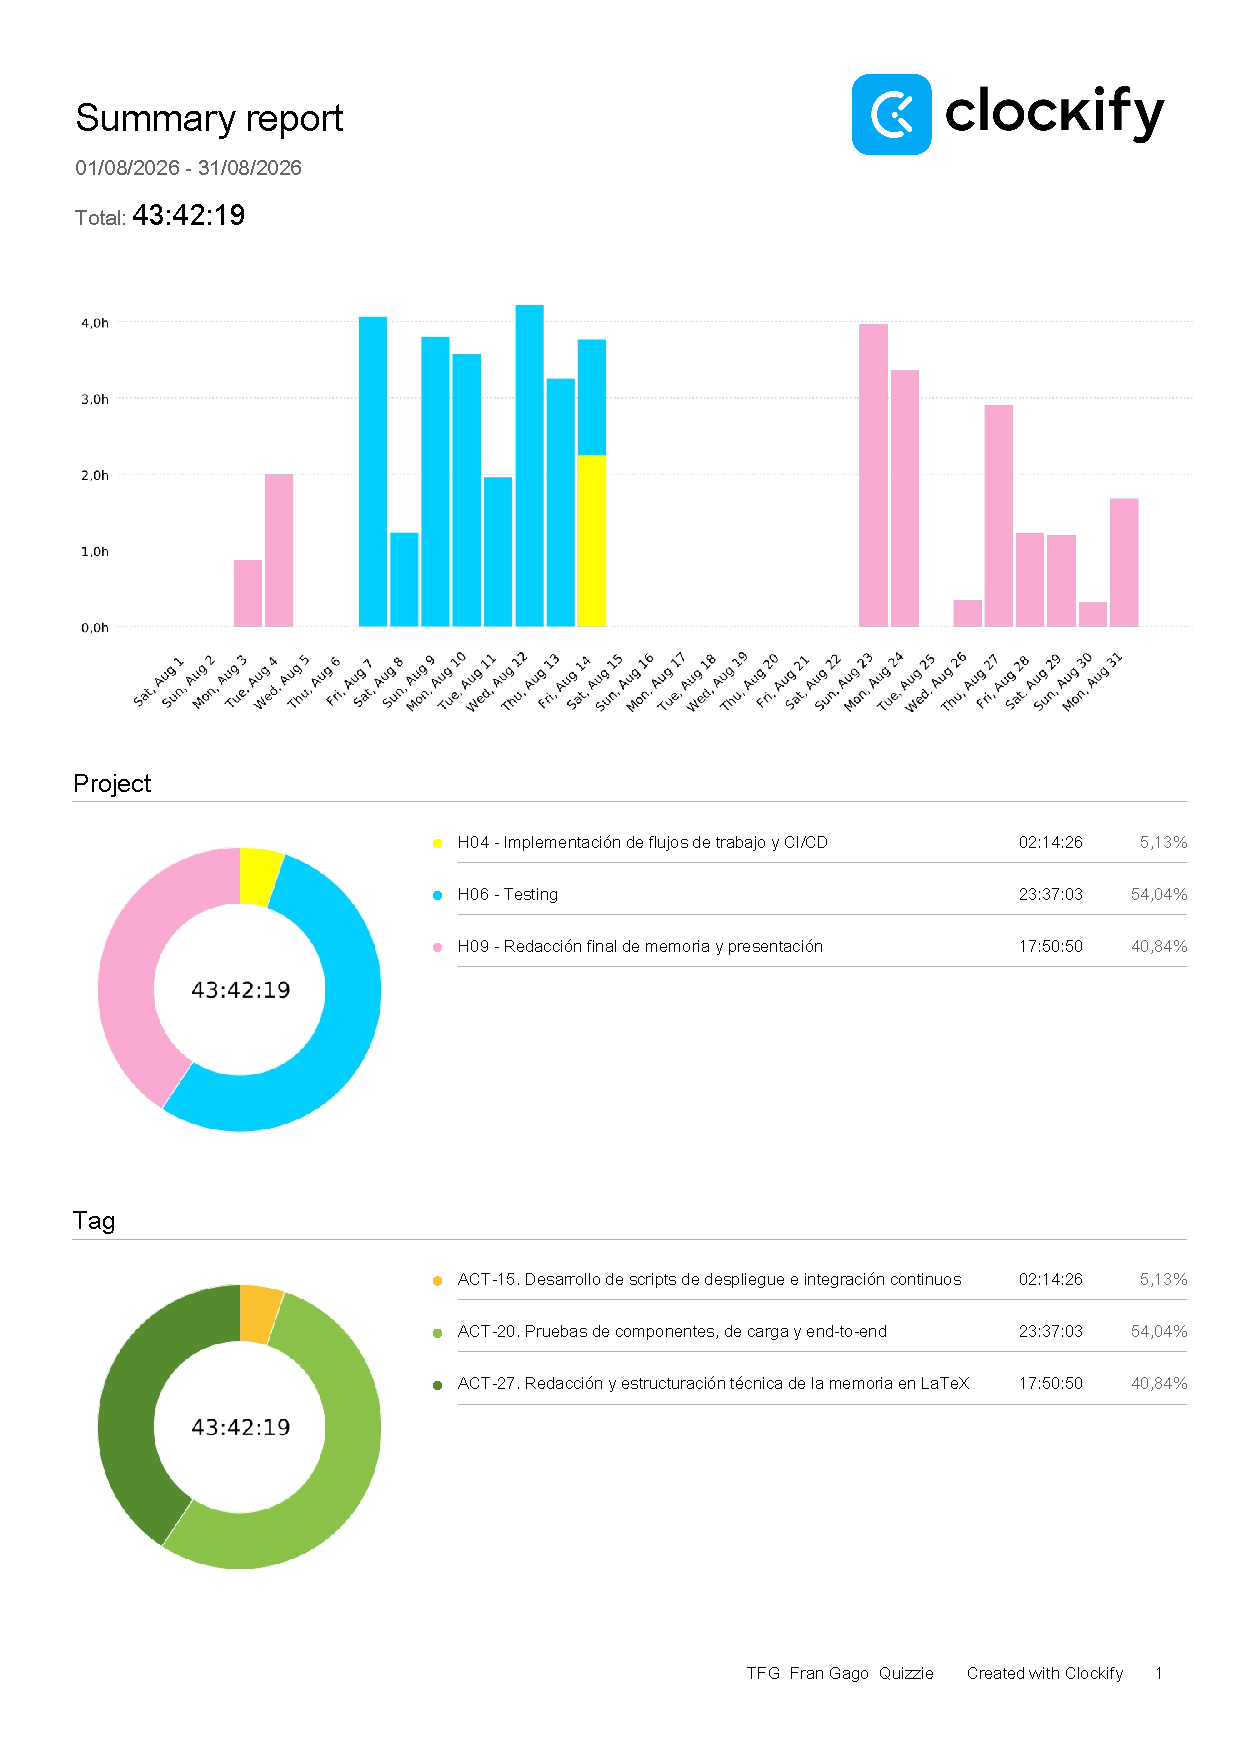
\includepdf[
    pages=-,
    scale=0.85,
    pagecommand={}
]{assets/informe_clockify.pdf}
\end{appendices}


    % Bibliografía
    \bibliographystyle{unsrtnat}
    \bibliography{conferencias,articulos,reportes,libros,enlaces}


% Fin del documento
\end{document}
